\documentclass[10pt]{book}

\usepackage{cdtUsecases}
\usepackage{txfonts}
\bibliographystyle{ieeetr} % Estilo IEEE

\title{Entregable C2-EP2\bigskip\\Nombre del Proyecto}
\subtitle{Componente 2 Iteración 2 Especificación del proyecto}
\author{Nombre del equipo o consultoría}
\organization{Escuela Superior de Cómputo, IPN}
\showInstrucciones
\date{\color{red}Borrador del 21 de febrero del 2017\\(para revisión)}
%\date{\color{green}Version 1.0}

%%%%%%%%%%%%%%%%%%%%%%%%%%%%%%%%%%%%%%%%%%%%%%%%%%%%%%%%%%%%%%%%
\begin{document}

%\ThisLRCornerWallPaper{1}{theme/bannerAzul} 
\maketitle
\thispagestyle{empty}


\frontmatter
\tableofcontents
\listoffigures 
\listoftables

% 
%=========================================================
%\chapter{Project Charter}

\newcommand{\ESCOMPchSec}[1]{\rowcolor{colorAgua}\multicolumn{4}{|c|}{\bf #1}\\\hline}
\newcommand{\ESCOMPchItem}[2]{{\bf {#1}} & \multicolumn{3}{p{.66\textwidth}|}{#2}\\\hline}
\newcommand{\ESCOMPchSubItem}[3]{{\bf {#1}} & {#2} & \multicolumn{2}{p{.44\textwidth}|}{#3}\\\hline}
\newcommand{\ESCOMPchSubSubItem}[4]{{\bf {#1}} & {#2} & {#3}& {#4}\\\hline}

\cleardoublepage
{\centering{\Huge Project Charter}\bigskip\\}
\begin{table}[hptb!] 
%\renewcommand\thetable{i}
\begin{tabular}{|p{.22\textwidth} |p{.22\textwidth} |p{.22\textwidth} |p{.22\textwidth} |}
	\hline
	\ESCOMPchItem{Proyecto:}{CVE, Nombre proyecto.}
	\ESCOMPchItem{Responsable:}{Empresa, Nombre del responsable, cargo, Firma.}
	\ESCOMPchItem{Autoriza:}{Empresa, Nombre del responsable, cargo, Firma.}
	\ESCOMPchItem{Background/Contexto:}{Descripción breve del contexto, no mas de 3 líneas.}
	\ESCOMPchItem{Beneficios esperados:}{Principales beneficios al término del proyecto.}
	\ESCOMPchItem{Costo estimado:}{\$ 2,350,700.00 $\pm$ 13\% (por ejemplo.)}
	\ESCOMPchSubSubItem{Fecha de inicio:}{Fecha}{\bf Fecha de término:}{Fecha.}
	\ESCOMPchItem{Objetivo:}{Objetivo general del proyecto.}
	\ESCOMPchSec{Entregables Principales}
	\ESCOMPchSubItem{}{Clave-Nombre}{descripción del entregable}
	\ESCOMPchSubItem{}{Clave-Nombre}{descripción del entregable}
	\ESCOMPchSubItem{}{...}{}
	\ESCOMPchSec{Alcance del proyecto}
	\ESCOMPchItem{Incluye:}{
		\begin{Titemize}
			\Titem Elemento 1 del alcance que incluye.
			\Titem ...
		\end{Titemize}
	}
	\ESCOMPchItem{Excluye:}{
		\begin{Titemize}
			\Titem Elemento 1 del alcance que incluye.
			\Titem ...
		\end{Titemize}
	}
	\ESCOMPchItem{Criterio de éxito:}{Indicador clave de término del proyecto}
	\ESCOMPchItem{Metodología:}{Metodología o metodologías que se utilizan (dos renglones o lista de no mas de 7)}
	\ESCOMPchSec{Datos de contacto}
	\ESCOMPchItem{Project Manager:}{Nombre, Tel, correo, etc.}
	\ESCOMPchItem{Project owner:}{Nombre, Tel, correo, etc.}
	\ESCOMPchItem{...}{}
	\ESCOMPchItem{Riesgos y peligros:}{
		\begin{Titemize}
			\Titem Riesgo o peligro identificado.
			\Titem ...
		\end{Titemize}
	}
	\ESCOMPchItem{Supuestos:}{
		\begin{Titemize}
			\Titem Suposiciones hechas de las que depende el éxito del proyecto.
			\Titem ...
		\end{Titemize}
	}
	\ESCOMPchItem{Restricciones y dependencias:}{
		\begin{Titemize}
			\Titem Restricciones del proyecto.
			\Titem ...
		\end{Titemize}
	}
	\ESCOMPchSec{Supervisión}
	\ESCOMPchSubItem{Juntas:}{(Nombre de la(s) persona(s)),}{ reporta a (Nombre de la(s) persona(s))}
	\ESCOMPchSubItem{Dudas:}{(Nombre de la(s) persona(s)),}{ reporta a (Nombre de la(s) persona(s))}
	\ESCOMPchSubItem{Avances:}{(Nombre de la(s) persona(s)),}{ reporta a (Nombre de la(s) persona(s))}
	\ESCOMPchSubItem{...}{}{}
\end{tabular}
	\caption{Resumen del proyecto}
	\label{tbl:projectCharter}
\end{table}


\mainmatter 
%\LRCornerWallPaper{1}{theme/plecaAyD} 

%%%%%%%%%%%%%%%%%%%%%%%%%%%%%%%%%%%%%%%%%%%%%%%%%%%%%%%%%%%%%%%%

\chapter{Análisis}

%=========================================================
%%=========================================================
\chapter{Introducción}


\cdtInstrucciones{
	Presentar el documento, indicando su contenido, a quien va dirigido, quien lo realizó, por que razón, dónde y cuando. \\
}
	Este documento contiene la Especificacion del ptoyecto ``{\em Nombre del proyecto}'' correspondiente al trabajo realizado en el semestre 2016-2017-2 para la materia de Análisis y diseño orientado a objetos en el grupo 2CV9 por el equipo {\em Nombre del equipo}.

%---------------------------------------------------------
\section{Presentación}


\cdtInstrucciones{
	Indique el propósito del documento y las distintas formas en que puede ser utilizado.\\
}
	Este documento contiene la especificación de los requerimientos del usuario y del sistema del sistema a desarrollar. Tiene como objetivo establecer la naturaleza y funciones del sistema para su evaluación al final del semestre. Este documento debe ser aprobado por los principales responsables del proyecto.
	
	Este documento es el C2-EP1 del proyecto ``{\em Nombre del proyecto}''.
	
%---------------------------------------------------------
\section{Organización del contenido}

	En el capítulo \ref{cap:reqUsr} ...
	
	En el capítulo \ref{cap:reqSist} ...

%---------------------------------------------------------
\section{Notación, símbolos y convenciones utilizadas}

	Los requerimientos funcionales utilizan una clave RFX, donde:
	
\begin{description}
	\item[X] Es un número consecutivo: 1, 2, 3, ...
	\item[RF] Es la clave para todos los {\bf R}equerimientos {\bf F}uncionales.
\end{description}

	Los requerimientos del usuario utilizan una clave RUX, donde:
	
\begin{description}
	\item[X] Es un número consecutivo: 1, 2, 3, ...
	\item[RU] Es la clave para todos los {\bf R}equerimientos del {\bf U}suario.
\end{description}

	Además, para los requerimeitnos funcionales se usan las abreviaciones que se muestran en la tabla~\ref{tbl:leyendaRF}.
\begin{table}[hbtp!]
	\begin{center}
    \begin{tabular}{|r l|}
	    \hline
    	{\footnotesize Id} & {\footnotesize\em Identificador del requerimiento.}\\
    	{\footnotesize Pri.} & {\footnotesize\em Prioridad}\\
    	{\footnotesize Ref.} & {\footnotesize\em Referencia a los Requerimientos de usuario.}\\
    	{\footnotesize MA} & {\footnotesize\em Prioridad Muy Alta.}\\
    	{\footnotesize A} & {\footnotesize\em Prioridad Alta.}\\
    	{\footnotesize M} & {\footnotesize\em Prioridad Media.}\\
    	{\footnotesize B} & {\footnotesize\em Prioridad Baja.}\\
    	{\footnotesize MB} & {\footnotesize\em Prioridad Muy Baja.}\\
		\hline
    \end{tabular} 
    \caption{Leyenda para los requerimientos funcionales.}
    \label{tbl:leyendaRF}
	\end{center}
\end{table}
% !TeX root = ../ejemplo.tex

\section{Sistema operativo}

Ahora bien, para que una aplicación móvil funcione correctamente, es fundamental comprender el papel crucial que desempeña el sistema operativo en los dispositivos.
Los sistemas operativos son el software principal de cualquier dispositivo móvil o computadora, estos comienzan a funcionar desde el primer momento que el dispositivo es encendido y son los encargados de preparar e iniciar todos los procesos principales, estructuras importantes y todas las herramientas que hacen que el dispositivo pueda comunicarse e interactuar con quien lo utiliza, y viceversa [11],[12].
En otras palabras, un sistema operativo es el software que se encarga de ofrecer una interfaz para interactuar al usuario, gestionar la seguridad del dispositivo, el acceso a los periféricos conectados y administrar la memoria asignada, los procesos, los recursos, las tareas y las actualizaciones y versiones de sí mismo o de otro software [11],[12]. 
Los sistemas operativos se dividen según su entorno (móviles o de computadora):

\subsection{Sistemas operativos móviles}

“Son los que se han creado y desarrollado para dispositivos móviles, fundamentalmente móviles y tablets, pero también relojes inteligentes. Los más conocidos son Android y iOS” [12].

\subsection{Sistema operativo android}

\begin{list}{}%
    {\setlength{\leftmargin}{1cm}\setlength{\rightmargin}{1cm}}
    \item\relax
    \small
    Android es reconocido como el sistema operativo más utilizado en el mundo debido a su versatilidad. Su diseño de código abierto permite a los desarrolladores crear aplicaciones personalizadas y a los fabricantes de hardware adaptarlo para sus dispositivos específicos. Además, su constante evolución garantiza compatibilidad con las últimas tecnologías y características [13].
    \end{list}

\subsection{Principales características Android}

    \begin{list}{}%
    {\setlength{\leftmargin}{1cm}%
     \setlength{\rightmargin}{1cm}%
     \setlength{\itemsep}{0.5\baselineskip}%
     \setlength{\parsep}{0pt}}
     
    \item\relax
    \small
    \textbf{Interfaz personalizable:} Android permite a los fabricantes y usuarios personalizar la apariencia y funcionalidad del sistema (pantalla de inicio, iconos y estructura gráfica) [14]. 
    
    \item\relax
    \small
    \textbf{Google Play y su ecosistema:} Android ofrece acceso a la Google Play Store, la cual es una tienda virtual de Google que permite a los usuarios descargar y subir aplicaciones de todo tipo, siempre y cuando cumplan con las normas de seguridad y calidad. Además, esta tienda facilita la integración con los servicios de Google, los cuales son usados con extrema frecuencia [14].
    
    \item\relax
    \small
    \textbf{Seguridad:} Android incluye Google Play Protect, que es una aplicación encargada de analizar otras aplicaciones y proteger el dispositivo. Además, esta ofrece actualizaciones frecuentes y permite al usuario decidir qué datos compartir con el desarrollador mediante el uso de permisos [14].
    
    \end{list}

\subsection{Sistemas operativo iOS}

\begin{list}{}%
    {\setlength{\leftmargin}{1cm}\setlength{\rightmargin}{1cm}}
    \item\relax
    \small
    iOS es un sistema operativo lanzado y utilizado por Apple. Su nombre proviene de iPhone OS. Es decir, iPhone Operative System o Sistema Operativo de iPhone. Utilizando las siglas, iOS. Se lanzó originalmente para el teléfono de la marca, aunque también se ha utilizado durante años en otros dispositivos de la compañía como en algunos de los reproductores de música iPod o en las tabletas iPad (hasta la llegada de iPadOS) [15].

    Se trata de un sistema cerrado que no puedes utilizar salvo en dispositivos de marca Apple. La gran diferencia con Android es esta: el sistema operativo de Google puede instalarse en infinidad de teléfonos de todas las marcas, pero iOS es un sistema cerrado y exclusivo para los aparatos de la marca de Cupertino. No para los demás. Al igual que otros sistemas operativos móviles, iOS nos permite instalar aplicaciones para añadir funciones a las que vienen por defecto en el smartphone [15].

\end{list}
    
\subsection{Principales características iOS}


    \begin{list}{}%
        {\setlength{\leftmargin}{1cm}%
         \setlength{\rightmargin}{1cm}%
         \setlength{\itemsep}{0.5\baselineskip}%
         \setlength{\parsep}{0pt}}
         
        \item\relax
        \small
        \textbf{Interfaz Intuitiva y Optimización:} iOS ofrece una interfaz amigable y visualmente atractiva, con navegación mediante gestos simples y optimiza el rendimiento para el hardware específico de Apple [16].
 
        
        \item\relax
        \small
        \textbf{Seguridad y Privacidad de Alto Nivel:} Apple prioriza la seguridad a través de características como encriptación de extremo a extremo, autenticación biométrica y su sistema de App Sandbox, que aísla cada aplicación para evitar el acceso no autorizado a información sensible [16].

        
        \item\relax
        \small
        \textbf{App Store Segura:} Las aplicaciones en iOS deben cumplir con estrictos estándares de seguridad para ser aprobadas en la App Store. Apple realiza auditorías regulares para asegurar que las aplicaciones estén libres de malware y respeten la privacidad de los usuarios [16].
        
        \end{list}

\subsection{Comparando Android e iOS}

\begin{table}[ht]
    \centering
    \begin{tabular}{|p{3cm}|p{5cm}|p{5cm}|}
    \hline
    \textbf{Criterio} & \textbf{Android} & \textbf{iOS} \\ \hline
    Lenguajes de programación & Kotlin & Swift \\ \hline
    IDE (Entorno de desarrollo) & Android Studio & Xcode \\ \hline
    Plataforma de distribución & Google Play Store & App Store \\ \hline
    Documentación y comunidad & Acceso más flexible, pero con más variabilidad entre dispositivos. & Mejor integración con el hardware de Apple (optimización). \\ \hline
    Distribución de aplicaciones & Publicación rápida, sin aprobación previa. & Necesita aprobación antes de publicación (más controlado). \\ \hline
    Costos de desarrollo & Sin costos de registro anual. & Licencia de desarrollador de 99 dólares al año. \\ \hline
    Mercado objetivo & Mercado más amplio, con una variedad de dispositivos (bajos, medios y altos). & Usuarios de Apple, con dispositivos limitados. \\ \hline
    Desarrollo multiplataforma & Ecosistema más diverso con diferentes marcas y modelos de dispositivos. & Integración total entre dispositivos Apple (iPhone, iPad, Mac, etc.). \\ \hline
    Actualizaciones & Las actualizaciones son más lentas y dependen del fabricante. & Actualizaciones frecuentes y rápidas para todos los usuarios. \\ \hline
    Comunidad y recursos & Comunidad más grande con más recursos, tutoriales y soporte. & Comunidad muy activa pero más pequeña comparada con Android, además de que los tutoriales son más avanzados y poco amigables a los principiantes. \\
    \hline
    \end{tabular}
    \caption{Comparación entre Android y iOS.}
    \label{tab:Tabla1}
\end{table}


    Analizando las características de estos 2 sistemas operativos, decidimos enfocar nuestros esfuerzos en el desarrollo de una aplicación para Android, ya que, nuestro presupuesto es limitado y el tiempo de desarrollo es ajustado, esta plataforma nos ofrece varias ventajas. En primer lugar, Android tiene una cuota de mercado mucho más amplia, lo que nos permitirá llegar a un público más amplio sin tener que depender de un grupo cerrado como es el de iOS, esto es de suma importancia porque necesitamos maximizar el impacto de nuestra aplicación alcanzando la mayor cantidad de usuarios posible para que la mayor parte de los alumnos y profesores puedan usar la aplicación.
    Otro factor importante es el costo. Publicar una aplicación en la App Store de iOS requiere una tarifa anual de 99 dólares, algo que no podemos permitirnos con el presupuesto actual, por otro lado, Android solo requiere un pago único de 25 dolares para registrar nuestra cuenta de desarrollador, lo cual nos deja más recursos para otras áreas del proyecto, además, la distribución de la aplicación en Google Play es mucho más rápida y sencilla, ya que no tenemos que pasar por un proceso de revisión tan estricto como el de iOS, esto nos permitirá lanzar nuestra aplicación en menos tiempo, algo que es crucial dado el tiempo limitado con el que contamos.
    Por ultimo Android es compatible con Python esto es un punto clave en nuestra decisión porque ya que planeamos usar Python para implementar el servidor de la aplicación y este nos facilita la implementación de funciones como; procesamiento de datos e imágenes, algoritmos de aprendizaje automático y técnicas de reconocimiento facial y redes neuronales (cabe recalcar que Android es compatible con OpenCV).
    

\subsection{Sistemas operativos para computadoras}

Son los que se han creado y desarrollado para que funcionen en computadoras de escritorio y portátiles. Los más conocidos son Windows, macOS y Unix.

\subsection{Sistema operativo Windows}

\begin{list}{}%
    {\setlength{\leftmargin}{1cm}\setlength{\rightmargin}{1cm}}
    \item\relax
    \small

El sistema operativo Windows, desarrollado por Microsoft, es uno de los sistemas operativos más populares y ampliamente utilizados en el mundo. Ofrece una interfaz gráfica intuitiva que permite a los usuarios interactuar con el hardware y software de sus computadoras de manera eficiente [17].
La estructura de Windows se basa en capas, donde cada capa cumple una función específica. La capa más baja es el kernel, que se encarga de gestionar los recursos de hardware y proporcionar servicios básicos al sistema operativo. Por encima del kernel se encuentran los controladores de dispositivo, que permiten la comunicación entre el hardware y el sistema operativo [17].
Además de estas capas fundamentales, Windows cuenta con una amplia gama de servicios y aplicaciones que ofrecen funcionalidades adicionales a los usuarios. Estas aplicaciones incluyen el Explorador de Windows, que permite a los usuarios navegar por los archivos y carpetas de su computadora, y el Panel de Control, que proporciona acceso a la configuración del sistema [17]. 

\end{list}


\subsection{CSistemas operativo macOS}

\begin{list}{}%
    {\setlength{\leftmargin}{1cm}\setlength{\rightmargin}{1cm}}
    \item\relax
    \small

Mac o MacOS, es el nombre del sistema operativo desarrollado por Apple para la línea de computadoras creados por la misma empresa. MacOS en sí mismo no es un sistema operativo, sino una familia de sistemas que han ido evolucionando a través de diferentes versiones con el paso del tiempo. La principal característica del sistema operativo Mac, es que éste está diseñado para funcionar de manera optimizada en equipos de Apple [18].
El sistema operativo Mac sigue la línea de compatibilidad de Apple, por lo que permite la comunicación entre MacOS y otros dispositivos creados por Apple como el iPad, appleTV, iPhone, etc [18].
Debido a su arquitectura, MacOS cuenta con un sistema de archivos propio, por lo que no puede procesar de forma nativa los archivos o programas con formatos usualmente empleados para Windows o Linux [18].

\end{list}


\subsection{Sistemas operativo Unix}

\begin{list}{}%
    {\setlength{\leftmargin}{1cm}\setlength{\rightmargin}{1cm}}
    \item\relax
    \small

Unix es un sistema operativo que nace a principios de los años 70, creado principalmente por Dennis Ritchie y Ken Thompson. Sus características técnicas principales son: su portabilidad, su capacidad multiusuario y multitarea, su eficiencia; su alta seguridad y su buen desempeño en tareas de red. Pero Unix, más que una marca, también es una filosofía que tiene por principios el minimalismo y el modularidad: hacer programas que hagan una sola cosa bien hecha y que, al comunicarse entre sí, ejecuten tareas más complejas.
Un sistema Unix puede dividirse en tres áreas básicas: 

        El núcleo del sistema operativo.

        El intérprete de comandos y algunos programas utilitarios.

        Lo demás que necesitas, como las aplicaciones de usuario o la interfaz gráfica, son paquetes adicionales.

Por sus características técnicas y su filosofía abierta, existen diversos sistemas operativos que se conocen como derivados de Unix o sistemas de la familia Unix [19].

\end{list}


\subsection{Comparando Windows, Linux y macOS}

\begin{table}[ht]
    \centering
    \begin{tabular}{|p{2cm}|p{5cm}|p{5cm}|p{5cm}|}
    \hline
    \textbf{Característica} & \textbf{Windows} & \textbf{Linux} & \textbf{macOS}\\ \hline

    Accesibilidad & Muy accesible, ampliamente disponible en PCs de todos los rangos de precios. & Requiere conocimientos técnicos, pero es gratis y disponible en una amplia gama de hardware. & Accesible solo en hardware Apple (más costoso). \\ \hline
    Herramientas de Desarrollo & Soporta una amplia gama de IDEs y plataformas de desarrollo. & Soporta herramientas como Visual Studio Code, PyCharm, Eclipse; excelente para desarrollo web, sistemas y servidores. & Excelente soporte para Xcode y terminal poderoso. \\ \hline
    Compatibilidad con Lenguajes & Amplia compatibilidad con lenguajes como Java, Python, JavaScript, C++, entre otros. & Compatible con casi todos los lenguajes, ideal para Python, C, C++, JavaScript, etc. & Compatible con todos los lenguajes principales, especialmente para desarrollo iOS (Swift, Objective-C). \\ \hline
    Soporte de Software & Compatible con la mayoría de las aplicaciones comerciales. & Menos compatibilidad con software comercial, pero excelente soporte para software libre y de código abierto. & Mejor compatibilidad con software de diseño y desarrollo exclusivo de Apple. \\ \hline
    Rendimiento & Rinde bien en la mayoría de las configuraciones, pero puede ser más pesado que Linux o macOS. & Suele ser más ligero y rápido en hardware modesto. & Gran rendimiento en hardware Apple, optimizado para su arquitectura. \\ \hline
    Costo & Varía dependiendo de la edición (Windows Home o Pro). & Totalmente gratuito. & Alto costo de hardware y software. \\ \hline
    Soporte de Python & Soporta bien Python, con muchas herramientas. & Ideal para Python, con herramientas avanzadas y administración de entornos virtuales. & Buen soporte para Python, con herramientas como Anaconda y entornos virtuales. \\ \hline
    Facilidad de Uso & Interfaz fácil de usar para la mayoría de usuarios, especialmente principiantes. & Requiere algo de conocimiento técnico para instalar y configurar, pero es muy flexible. &Intuitivo y fácil de usar, especialmente para usuarios de Apple. \\ \hline
    Desarrollo Móvil & Soporta desarrollo Android mediante Android Studio y otras herramientas. & Soporta Android Studio y desarrollo móvil para otras plataformas, pero no es ideal para iOS. & Ideal para desarrollo iOS (Xcode) y aplicaciones macOS. \\



    \hline
    \end{tabular}
    \caption{Comparación entre Android y iOS.}
    \label{tab:Tabla2}
    \end{table}

Conociendo las características de estos 3 sistemas operativos, decidimos optar por Windows como el sistema operativo principal para el desarrollo de nuestro proyecto, ya que, teniendo en cuenta nuestras limitaciones de presupuesto y tiempo, este sistema operativo nos ofrece ventajas importantes. En primer lugar, Windows es el sistema operativo más accesible para nosotros porque todo el equipo posee una computadora con este sistema operativo, por lo cual se nos facilita que nuestro equipo trabaje con estos equipos o si se requiere, se nos facilitaría adquirir nuevas computadoras sin que el costo sea una preocupación mayor.
Otro punto a favor que consideramos de Windows es la compatibilidad con una gran cantidad de herramientas de desarrollo ya que este sistema operativo ofrece soporte para una variedad de lenguajes de programación y es compatible con muchos de los entornos de desarrollo integrados (IDE). Esto nos permite utilizar las herramientas que ya conocemos o las que se ajustan mejor a nuestras necesidades sin tener que invertir tiempo en aprender nuevas plataformas, además, Windows es compatible con una gran variedad de software comercial y aplicaciones específicas, como las herramientas de diseño gráfico y edición, que son necesarias para el diseño de la aplicación y sus componentes gráficos.
Cabe mencionar que Linux es una excelente opción por su flexibilidad y la capacidad extra de los servidores, sin embargo, la escala del proyecto no es tan masiva, por lo que, decidimos que no era la mejor opción para nuestro proyecto debido a que requiere un conocimiento más avanzado y específico para configurar y administrar, también la curva de aprendizaje retrasaría el progreso porque poseemos una nula experiencia trabajando con este sistema operativo. Además, aunque Linux es gratuito y ligero, su compatibilidad con software comercial y aplicaciones de terceros no es tan robusta como la de Windows, lo que nos presenta problemas para aspectos del desarrollo.
Por otro lado, macOS tiene ventajas notables, como su optimización y rendimiento en hardware Apple, pero el costo del hardware y la limitación de solo estar disponible para dispositivos Apple lo hacen menos accesible para nuestro presupuesto. Además, aunque macOS es excelente para el desarrollo de aplicaciones iOS/macOS, no es tan versátil como Windows en cuanto a compatibilidad con diversas herramientas de desarrollo y software de terceros.


% !TeX root = ../ejemplo.tex

\section{Lenguaje de programación}

Una vez establecido el sistema operativo que vamos a usar, nos interesa establecer que es un lenguaje de programación.
\begin{list}{}%
    {\setlength{\leftmargin}{1cm}\setlength{\rightmargin}{1cm}}
    \item\relax
    \small
En términos generales, un lenguaje de programación es una herramienta que permite desarrollar software o programas para computadora. Los lenguajes de programación son empleados para diseñar e implementar programas encargados de definir y administrar el comportamiento de los dispositivos físicos y lógicos de una computadora. Lo anterior se logra mediante la creación e implementación de algoritmos de precisión que se utilizan como una forma de comunicación humana con la computadora \cite{CitaD10}.

A grandes rasgos, un lenguaje de programación se conforma de una serie de símbolos y reglas de sintaxis y semántica que definen la estructura principal del lenguaje y le dan un significado a sus elementos y expresiones \cite{CitaD10}.
\end{list}
Estos se dividen en 3 tipos: lenguajes máquina, lenguajes de bajo nivel y lenguajes de alto nivel.


\subsection{Lenguajes máquina}

\begin{list}{}%
    {\setlength{\leftmargin}{1cm}\setlength{\rightmargin}{1cm}}
    \item\relax
    \small

Es el sistema de códigos interpretable directamente por un circuito microprogramable, como el microprocesador de una computadora. Este lenguaje se compone de un conjunto de instrucciones que determinan acciones que serán realizadas por la máquina. Y un programa de computadora consiste en una cadena de estas instrucciones de lenguaje de máquina (más los datos). Normalmente estas instrucciones son ejecutadas en secuencia, con eventuales cambios de flujo causados por el propio programa o eventos externos. El lenguaje máquina es específico de cada máquina o arquitectura de la máquina, aunque el conjunto de instrucciones disponibles pueda ser similar entre ellas \cite{CitaD10}.

\end{list}

\subsection{Lenguajes de alto nivel}

\begin{list}{}%
    {\setlength{\leftmargin}{1cm}\setlength{\rightmargin}{1cm}}
    \item\relax
    \small

Un lenguaje de programación de bajo nivel es el que proporciona poca o ninguna abstracción del microprocesador de una computadora. Consecuentemente, su trasladado al lenguaje máquina es fácil. El término ensamblador (del inglés assembler) se refiere a un tipo de programa informático encargado de traducir un archivo fuente, escrito en un lenguaje ensamblador, a un archivo objeto que contiene código máquina ejecutable directamente por la máquina para la que se ha generado \cite{CitaD10}. 

\end{list}

\subsection{Lenguajes de bajo nivel}

\begin{list}{}%
    {\setlength{\leftmargin}{1cm}\setlength{\rightmargin}{1cm}}
    \item\relax
    \small

Los lenguajes de programación de alto nivel se caracterizan porque su estructura semántica es muy similar a la forma como escriben los humanos, lo que permite codificar los algoritmos de manera más natural, en lugar de codificarlos en el lenguaje binario de las máquinas, o a nivel de lenguaje ensamblador \cite{CitaD10}. 

\end{list}

Entre estos tipos de lenguajes nos interesa los lenguajes de alto nivel ya que para el proyecto estamos considerando el uso de Python, Java y Kotlin, que son considerados lenguajes de alto nivel. Concretamente Python es un lenguaje multiparadigma que puede ser estructurado como si se usara la programación orientada a objetos, Java usa la programación orientada a objetos y Kotlin puede trabajar con esta orientación por lo que antes de definir qué son estos dos lenguajes es de vital importancia definir qué es la “programación orientada a objetos”.


\subsection{Programación orientada a objetos}

\begin{list}{}%
    {\setlength{\leftmargin}{1cm}\setlength{\rightmargin}{1cm}}
    \item\relax
    \small

La programación orientada a objetos (POO) es un modelo de programación informática que organiza el diseño del software en torno a datos u objetos, en lugar de funciones y lógica. Un objeto puede definirse como un campo de datos que tiene unos atributos y comportamientos únicos\cite{CitaD11}.
Los ejemplos de un objeto pueden ir desde entidades físicas, como un ser humano que se describe por propiedades como el nombre y la dirección, hasta pequeños programas informáticos, como los widgets\cite{CitaD11}.
La POO se centra en los objetos que los desarrolladores quieren manejar, en lugar de la lógica necesaria para hacerlo. Este enfoque de la programación es muy adecuado para programas grandes, complejos y que se actualizan o mantienen activamente\cite{CitaD11}.
Esto incluye programas para la producción y el diseño web, así como aplicaciones móviles\cite{CitaD11}.

\end{list}

\subsection{Python}

\begin{list}{}%
    {\setlength{\leftmargin}{1cm}\setlength{\rightmargin}{1cm}}
    \item\relax
    \small

En términos técnicos, Python es un lenguaje de programación de alto nivel, orientado a objetos, con una semántica dinámica integrada, principalmente para el desarrollo web y de aplicaciones informáticas, o a nivel de lenguaje ensamblador\cite{CitaD12}.
Python es relativamente simple, por lo que es fácil de aprender, ya que requiere una sintaxis única que se centra en la legibilidad. Los desarrolladores pueden leer y traducir el código Python mucho más fácilmente que otros lenguajes\cite{CitaD12}.
Por tanto, esto reduce el costo de mantenimiento y de desarrollo del programa porque permite que los equipos trabajen en colaboración sin barreras significativas de lenguaje y experimentación\cite{CitaD12}.
Además, soporta el uso de módulos y paquetes, lo que significa que los programas pueden ser diseñados en un estilo modular y el código puede ser reutilizado en varios proyectos. Una vez se ha desarrollado un módulo o paquete, se puede escalar para su uso en otros proyectos, y es fácil de importar o exportar\cite{CitaD12}.
Por otro lado, uno de los beneficios más importantes de Python es que tanto la librería estándar como el intérprete están disponibles gratuitamente, tanto en forma binaria como en forma de fuente\cite{CitaD12}.
Tampoco hay exclusividad, ya que Python y todas las herramientas necesarias están disponibles en todas las plataformas principales \cite{CitaD12}.

\end{list}


\subsection{Java}

\begin{list}{}%
    {\setlength{\leftmargin}{1cm}\setlength{\rightmargin}{1cm}}
    \item\relax
    \small

Java es un lenguaje orientado a objetos; es decir que organiza el trabajo en torno a objetos en lugar de funciones y lógica. Las aplicaciones móviles y herramientas de software, incluidos los mundialmente famosos Amazon, Spotify y Minecraft, se basan en Java.
Java tiene dos propiedades que determinan qué tareas se pueden resolver con él.
Java es un lenguaje de programación orientado a objetos (POO). Toda interacción en él se produce a través de objetos. Estas entidades se describen en código y se les enseña a interactuar entre sí. Como resultado, un programa de estilo orientado a objetos consta de bloques separados que son fácilmente extensibles y escalables. \cite{CitaD13}

\end{list}

Y java tiene la capacidad de interpretar y compilar, es decir tiene un intérprete que se dedica a leer cada línea de código una por una y ejecutarla sin traducirla a lenguaje máquina y además puede transformar su código  a lenguaje máquina y hacer que el procesador lo compile traducido \cite{CitaD13}. 


\subsection{Kotlin}

Kotlin es un lenguaje de alto nivel debido a su abstracción respecto al hardware y la plataforma subyacente. Esto significa que permite a los desarrolladores escribir código sin preocuparse por la gestión de memoria o las interacciones directas con el sistema operativo o el hardware, lo que mejora la productividad y la legibilidad del código, además, este es estáticamente tipado, lo que implica que los tipos de las variables se definen en tiempo de compilación, lo que permite detectar errores antes de ejecutar el programa. Este se usa principalmente en el desarrollo de aplicaciones Android, donde es el lenguaje recomendado por Google \cite{CitaD14}.

Con la información anterior se puede explicar porque consideramos estos tres lenguajes de programación; Primero estos tres lenguajes poseen una misma orientación lo cual nos ayuda a que el desarrollo del proyecto sea más conciso y fácil, después estos son lenguajes de alto nivel que tienen una buena legibilidad lo que le permite al equipo entender de manera más sencilla el trabajo de los demás integrantes, también pueden ser conectados entre ellos de manera relativamente fácil y sobretodo su alta cantidad de bibliotecas de apoyo y su características de ser  estándares de desarrollo; en android (Kotlin), de desarrollo para servidores (Python) y Java para desarrollo web.
Otra razón por la que decidimos usar estos tres lenguajes de programación es por su compatibilidad con la API OpenCV la cual será una herramienta clave para el desarrollo de nuestro proyecto, por lo que es necesario explicar que es una API y qué es OpenCV.

% !TeX root = ../ejemplo.tex

\section{API}

\begin{list}{}%
    {\setlength{\leftmargin}{1cm}\setlength{\rightmargin}{1cm}}
    \item\relax
    \small

Una API, o interfaz de programación de aplicaciones, es un conjunto de reglas o protocolos que permiten que las aplicaciones de software se comuniquen entre sí para intercambiar datos, características y funcionalidades [25].
Las API simplifican y aceleran el desarrollo de software y aplicaciones permitiendo a los desarrolladores integrar datos, servicios y capacidades de otras aplicaciones, en lugar de desarrollarlas desde cero. Las API también ofrecen a los propietarios de aplicaciones una forma sencilla y segura de poner los datos y las funciones de sus aplicaciones a disposición de los departamentos de su organización. Los propietarios de aplicaciones también pueden compartir o comercializar datos y funciones con asociados de negocios o terceros [24].

\end{list}

\subsection{OpenCV}

\begin{list}{}%
    {\setlength{\leftmargin}{1cm}\setlength{\rightmargin}{1cm}}
    \item\relax
    \small

OpenCV, o Open Source Computer Vision Library, es una colección de más de 2500 algoritmos optimizados que facilitan el procesamiento de imágenes y la realización de diversas operaciones de vision computacional. Fundada por Intel en 2000 y con colaboración de múltiples empresas y desarrolladores, esta biblioteca es de fácil acceso y cuenta con una licencia BSD [25].
Siendo compatible con varios lenguajes de programación, incluido Python, Java y C++, OpenCV permite trabajar en múltiples plataformas y sistemas operativos. Esta biblioteca también destaca por su papel en el impulso de tecnologías emergentes como el deep learning [26].

\end{list}

Por último esta cuenta con muchos procesos y funciones que apoyan al reconocimiento facial, además de ser compatible con Python, Kotlin y Java y poseer una alta cantidad de tutoriales que rondan desde las integraciones básicas hasta procesos avanzados.

\subsection{Licencia BSD}

\begin{list}{}%
    {\setlength{\leftmargin}{1cm}\setlength{\rightmargin}{1cm}}
    \item\relax
    \small

"La licencia BSD, también conocida como licencia de distribución de software de Berkeley, es una popular licencia de código abierto que permite el libre uso, modificación y distribución de software [27]."

\end{list}

Ya con el sistema operativo y los lenguajes de programación establecidos, tenemos que especificar las herramientas que nos permitirán escribir, depurar y gestionar el código de manera eficiente. Estas herramientas son los entornos de desarrollo Integrados (IDE, por sus siglas en inglés), que proporcionan un conjunto de funciones como editores de código, depuradores, y compiladores.


% !TeX root = ../ejemplo.tex

\section{IDE}

Un entorno de desarrollo integrado (IDE) es un sistema de software para el diseño de aplicaciones que combina herramientas del desarrollador comunes en una sola interfaz gráfica de usuario (GUI). Generalmente, un IDE cuenta con las siguientes características \cite{CitaD18}:

\begin{list}{}%
    {\setlength{\leftmargin}{1cm}%
     \setlength{\rightmargin}{1cm}%
     \setlength{\itemsep}{0.5\baselineskip}%
     \setlength{\parsep}{0pt}}
     
    \item\relax
    \small
    \textbf{Editor de código fuente:} editor de texto que ayuda a escribir el código de software con funciones como el resaltado de la sintaxis con indicaciones visuales, el relleno automático específico para el lenguaje y la comprobación de errores a medida que se escribe el código \cite{CitaD18}.
    \textbf{Automatización de las compilaciones locales:} herramientas que automatizan las tareas sencillas y repetitivas como parte de la creación de una compilación local del software para que use el desarrollador, como la compilación del código fuente de la computadora en código binario, el empaquetado de ese código y la ejecución de pruebas automatizadas \cite{CitaD18}.
    \textbf{Depurador:} programa que sirve para probar otros programas y mostrar la ubicación de un error en el código original de forma gráfica \cite{CitaD18}.

\end{list}

Para nuestro proyecto ocuparemos el IDE llamado android studio.

\subsection{Android Studio}

\begin{list}{}%
    {\setlength{\leftmargin}{1cm}\setlength{\rightmargin}{1cm}}
    \item\relax
    \small

Android Studio es el entorno de desarrollo integrado (IDE) oficial para el desarrollo de aplicaciones del mismo OS. Se basa en IntelliJ IDEA, un entorno de desarrollo integrado de Java para software, e incorpora sus herramientas de desarrollo y edición de código \cite{CitaD19}.

Para respaldar el desarrollo de aplicaciones dentro del sistema operativo, Android Studio utiliza un sistema de compilación basado en Gradle, un emulador de Android, plantillas de código e integración de GitHub. Cada proyecto en Android Studio tiene una o más modalidades con código fuente y archivos de recursos \cite{CitaD19}.

\end{list}


\subsection{Gradle}

\begin{list}{}%
    {\setlength{\leftmargin}{1cm}\setlength{\rightmargin}{1cm}}
    \item\relax
    \small

Gradle, es una herramienta que permite la automatización de compilación de código abierto, la cual se encuentra centrada en la flexibilidad y el rendimiento. Los scripts de compilación de Gradle se escriben utilizando Kotlin DSL (Domain Specific Language) \cite{CitaD20}.
Gradle tiene una gran flexibilidad y nos deja hacer usos de otros lenguajes y no solo de Java, también cuenta con un sistema de gestión de dependencias muy estable. Gradle es altamente personalizable y rápido ya que completa las tareas de forma rápida y precisa reutilizando las salidas de las ejecuciones anteriores, sólo procesar las entradas que presentan cambios en paralelo \cite{CitaD20}.
Además es el sistema de compilación oficial para Android y cuenta con soporte para diversas tecnologías y lenguajes \cite{CitaD20}.

\end{list}


\subsection{GitHub}

\begin{list}{}%
    {\setlength{\leftmargin}{1cm}\setlength{\rightmargin}{1cm}}
    \item\relax
    \small

GitHub es una plataforma de desarrollo colaborativo que aloja proyectos en la nube utilizando el sistema de control de versiones llamado Git. Ayuda a los desarrolladores a almacenar y administrar el código llevando un registro de cambios. Generalmente el código es abierto, lo que permite realizar proyectos compartidos y mantener el seguimiento detallado de su progreso. La plataforma GitHub también funciona como red social conectando a los desarrolladores con los usuarios. Como usuario puedes descargar programas o aplicaciones, y de la misma manera puedes aportar a su desarrollo ofreciendo mejoras y discutir las cuestiones que te interesan en foros temáticos \cite{CitaD21}.
\end{list}

\subsection{Git}

\begin{list}{}%
    {\setlength{\leftmargin}{1cm}\setlength{\rightmargin}{1cm}}
    \item\relax
    \small

Git es un software de control de versiones diseñado por Linus Torvalds, el creador de Linux. El propósito de Git es llevar un registro de cambios y coordinar el trabajo de varias personas en un repositorio compartido. Desde su creación en 2005, este software llegó a convertirse en uno de los VCS más populares: según la encuesta de Stack Overflow (en inglés), más del noventa porciento de los desarrolladores usan Git en sus proyectos \cite{CitaD20}.
Git proporciona herramientas para un trabajo rápido y eficiente dentro de un equipo. El control de versiones permite a los desarrolladores descargar una copia del código fuente a sus repositorios locales (PC), realizar cambios y subir una versión nueva al repositorio compartido. Todas las modificaciones se guardan en versiones independientes, sin afectar el archivo original. Se pueden comparar cambios realizados, ver quién modificó el código y determinar en qué momento se introdujo un error para poder revertirlo. De esta forma todos los desarrolladores interesados en el proyecto tienen acceso al historial de modificaciones realizadas y pueden contribuir mejorando el código del software \cite{CitaD21}.

\end{list}

Esta última es una herramienta que tenemos planeada usar para el control de versiones en nuestro proyecto. 


%=========================================================
%=========================================================
\chapter{Modelo del Alcance}
\label{cap:reqUsr}

	En este capítulo se modela el alcance del sistema, se presentan  los requerimientos de usuario identificados y un diagrama de arquitectura de la solución propuesta junto con la especificación de plataforma correspondiente.

%---------------------------------------------------------

%---------------------------------------------------------


\section{Requerimientos de usuario}

En la siguiente tabla se enlistan los requerimientos de usuario identificados, estos corresponden a necesidades de los usuarios que harán uso del sistema. Se encuentran organizados por un Id único, el nombre del requerimiento, su descripción y su prioridad, que no es más que un análisis sobre su impacto en el desarrollo del sistema. 

\cdtInstrucciones{
	Identifique y describa los requerimientos funcionales del sistema señalando: id, nombre, descripción y prioridad.
}


\begin{requerimientosU}
	\FRitem{RU1}{Confirmar la asistencia a ETS}{Los alumnos quieren garantizar que su asistencia a la evaluación sea registrada.}{Alta}
	\FRitem{RU2}{Garantizar el acceso seguro y eficaz a las instalaciones.}{Los alumnos necesitan acceder a las instalaciones de forma rápida y segura, los días de aplicación a ETS.}{Alta}
	\FRitem{RU3}{Brindar alternativas para la identificación de alumnos.}{Los alumnos solicitan medios alternativos a los convencionales para autenticar su identidad.}{Media}
	\FRitem{RU4}{Confirmar la identidad de los alumnos presentes.}{Los docentes aplicadores quieren garantizar que los alumnos presentes estén inscritos al ETS}{Alta}
	\FRitem{RU5}{Reducir el tiempo del pase de lista.}{Los docentes aplicadores necesitan registrar la asistencia de los alumnos de manera rápida.}{Media}
	\FRitem{RU6}{Conocer los ETS inscritos.}{Los alumnos necesitan conocer los detalles de los ETS que van a presentar y el/la docente que lo impartirá.}{Media}
	\FRitem{RU7}{Conocer los ETS a impartir.}{Los docentes aplicadores necesitan conocer los detalles del ETS que supervisarán como el horario y lugar de aplicación.}{Media}
	\FRitem{RU8}{Conocer a los alumnos que presentaran ETS.}{Los docentes aplicadores necesitan conocer la información de los alumnos que están inscritos al ETS a aplicar.}{Media}
	\FRitem{RU9}{Conocer los horarios de aplicación de ETS.}{El personal de seguridad necesita conocer los horarios de aplicación de ETS para permitir o no la entrada de los estudiantes.}{Media}
	\FRitem{RU10}{Limitar el acceso a las instalaciones durante los ETS.}{El personal de seguridad necesita negar el acceso a la ESCOM a personas ajenas a la institución.}{Alta}
	\FRitem{RU11}{Registrar accesos a las instalaciones los días de aplicación de ETS}{El personal de seguridad necesita registrar los alumnos que acceden a las instalaciones para posterior consulta en caso de cualquier aclaración o imprevisto.}{Alta}
	\FRitem{RU12}{Comprobar los accesos a la institución en horarios oportunos.}{El personal de seguridad espera que los alumnos accedan en horarios congruentes con la aplicación de los ETS.}{Media}
	\FRitem{RU13}{Proteger la información personal.}{Los alumnos quieren mantener sus datos personales seguros.}{Alta}
	\FRitem{RU14}{Mantener separado las funciones y los datos de docentes y alumnos.}{Los docentes y alumnos esperan tener una ayuda personalizada para sus necesidades y no ver datos innecesarios.}{Media}
	\FRitem{RU15}{Mantener un recordatorio de eventos.}{Tanto los alumnos como docentes necesitan ser recordados sobre la información acerca de los ETS inscritos / asignados.}{Media}
	\FRitem{RU16}{Conocer las políticas de acceso a las instalaciones.}{Los alumnos quieren tener en claro cómo funciona el proceso de acceso a las instalaciones y qué documentos o pasos deben seguir para ingresar a las instalaciones los días de ETS.}{Media}
	\FRitem{RU17}{Minimizar los errores al verificar la identidad de los alumnos.}{Los docentes buscan minimizar la posibilidad de verificar de forma errónea la identidad de los alumnos.}{Alta}
	\FRitem{RU18}{Agilizar los procedimientos para la verificación de la identidad de los alumnos.}{Los docentes buscan minimizar los tiempos empleados en verificar la identidad de los alumnos presentes para la aplicación de los ETS.}{Alta}
	\FRitem{RU19}{Conocer fechas importantes del calendario escolar.}{Los alumnos, profesores y personal de seguridad necesitan conocer las fechas importantes del periodo escolar actual, incluyendo las relacionadas con los ETS.}{Baja}
	\FRitem{RU20}{Flexibilidad al aplicar ETS.}{Los profesores necesitan una alternativa que les permita delegar la responsabilidad de supervisar un ETS.}{Media}
	\FRitem{RU21}{Flexibilidad al aplicar ETS.}{Los profesores necesitan una alternativa que les permita delegar la responsabilidad de supervisar un ETS.}{Media}
	\FRitem{RU22}{Verificación de métodos de autenticación.}{Los alumnos requieren garantizar que los métodos de autenticación utilizados sean robustos y justos.}{Alta}
	\FRitem{RU23}{Control de ETS}{El personal de gestión escolar necesita gestionar la inscripción de los alumnos a los ETS.}{Media}
	\FRitem{RU24}{Control de trabajadores}{El personal de gestión escolar necesita gestionar los trabajadores adscritos al plantel educativo.}{Media}
	\FRitem{RU25}{Registro de alumnos.}{El personal de la DAE requiere dar de alta alumnos.}{Media}
	\FRitem{RU26}{Generación de credenciales de alumnos.}{El personal de la DAE requiere tomar fotografías de los alumnos para generar sus credenciales institucionales.}{Media}
	
	\caption{Requerimientos de usuario identificados.}
	{\footnotesize\em Para leer correctamente esta tabla vea la leyenda en la Tabla~\ref{tbl:leyendaRF} en la página~\pageref{tbl:leyendaRF}.}
	\label{tbl:reqFunc}	
	\end{requerimientosU}
	
   




%---------------------------------------------------------
\section{Especificación de plataforma}

A continuación se presenta la especificación de plataforma para aclarar el tipo de solución propuesta junto con un diagrama para establecer el patrón de arquitectura a utilizar.

\cdtInstrucciones{
	Coloque un diagrama y su descripción para aclarar el tipo de solución propuesta. \\
	
 En esta sección se debe aclarar:
	
\begin{description}
	\item[Tipo de sistema:] Aplicación híbrida, (aplicación móvil y sistema web para la gestión de estudiantes y exámenes)
	\item[Software requerido:] Python, SpringBoot, Java, Kotlin, bases de datos relacional PostgreSQL, base de datos vectorial (Pinecone).
	\item[Servicios:] De conexión, seguridad, firewall, respaldo de energía, redundancia, uso de raids, etc.
\end{description}
}

\begin{figure}[htbp!]
	\begin{center}
		\fbox{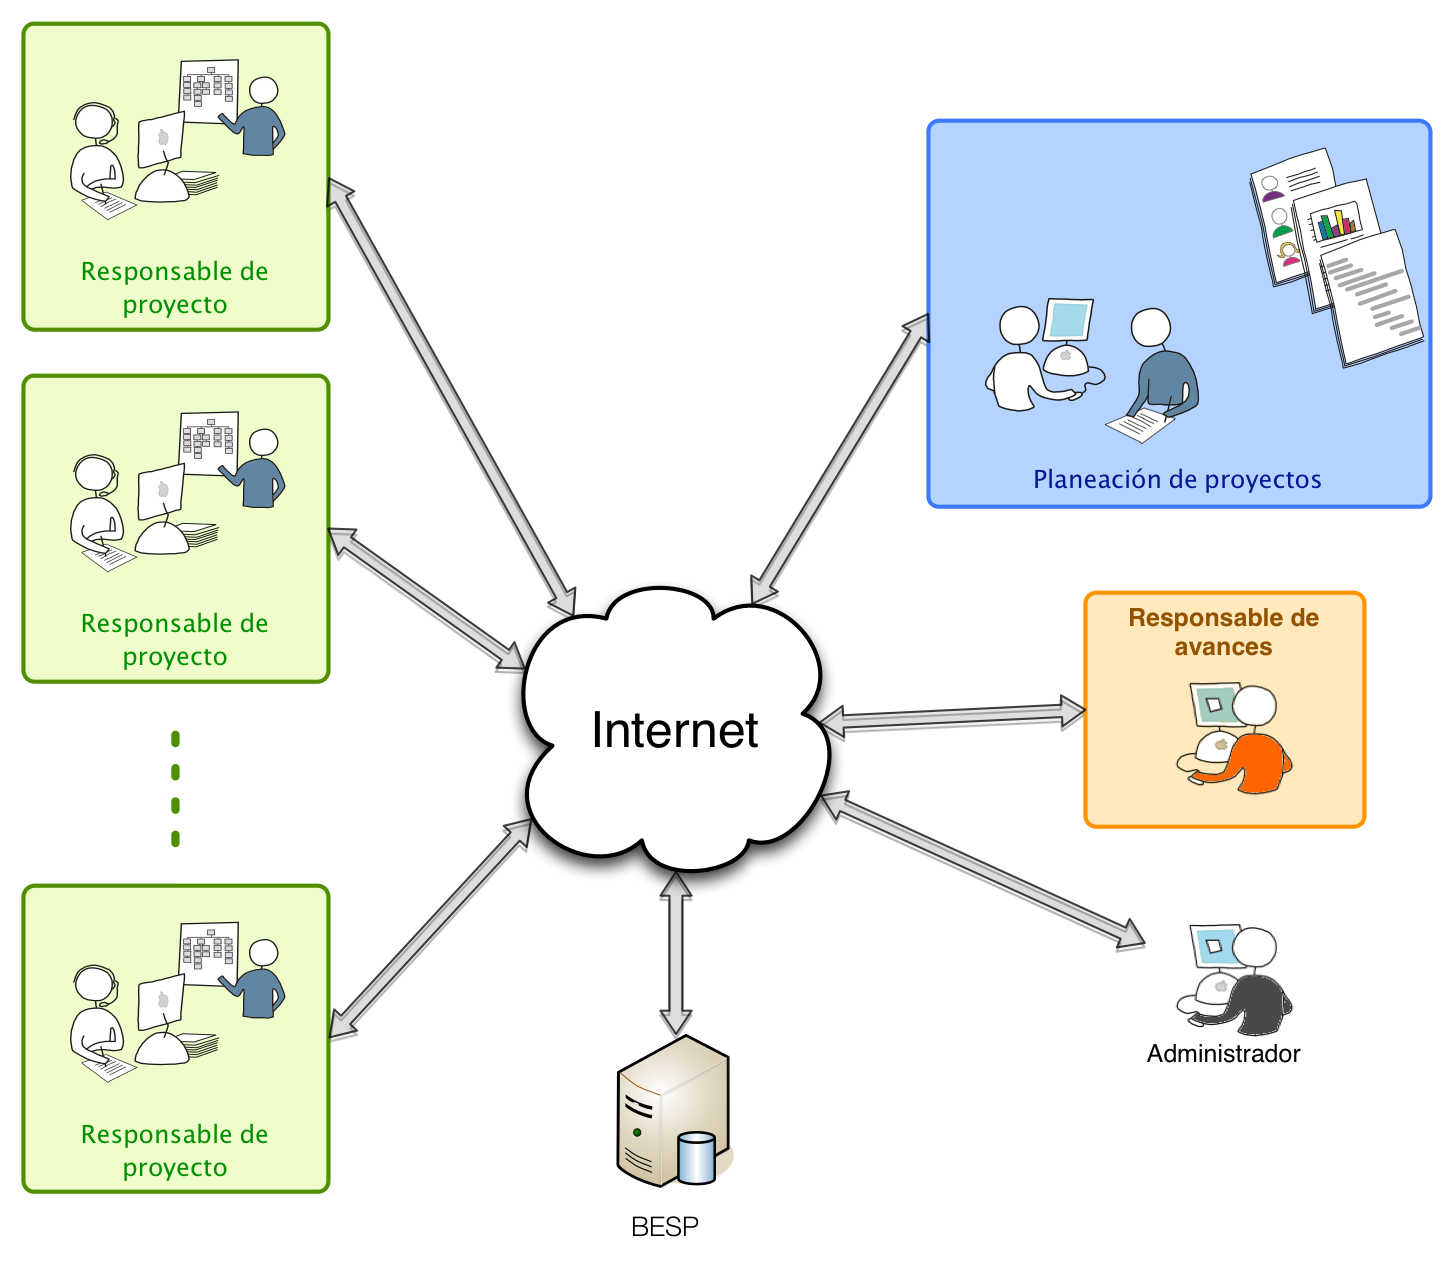
\includegraphics[width=.6\textwidth]{images/arquitectura}}
		\caption{Arquitectura del sistema.}
		\label{fig:arquitectura}
	\end{center}
\end{figure}

En la figura~\ref{fig:arquitectura} se describe la arquitectura general del sistema en la que se destaca el uso de un enfoque basado en micro-servicios, identificando los principales servicios que conforman la propuesta de solución y sus componentes principales.


%=========================================================
\section{Modelo del Negocio}	
\label{cap:reqSist}

	En está sección se modela la {\em Arquitectura del negocio} la cual está conformada por la Ontología del negocio ({\em Términos} y {\em Hechos del negocio}), Arquitectura de procesos y las {\em Reglas del negocio}. Primero se especifica brevemente el {\em Contexto} en el que los términos tienen significado.
		
	En las sección \ref{sec:terminosDeNegocio} se presentan los Términos del negocio a manera de Glosario y por último se presentan los Hechos del negocio a manera de relaciones entre términos del negocio.


%----------------------------------------------------------
\subsection{Contexto}

	\cdtInstrucciones{El contexto debe explicar bajo que ambiente los términos del negocio son aplicables y proporcionar información general para su comprensión inicial.\\}
	
	
%---------------------------------------------------------
\subsection{Términos del Negocio}
\label{sec:terminosDeNegocio}

\begin{description}
	% Ejemplo de un término literal.
	 \item[\hypertarget{tUnidadAcademica}{Unidad académica:}] Se refiere a la institución educativa en donde los usuarios se desenvuelven diariamente.
	
	\item[\hypertarget{tUnidadAprendizaje}{Unidad de aprendizaje:}] Son los elementos que componen un plan de estudios de alguna de las carreras ofertadas en la \hyperlink{tUnidadAcademica}{unidad académica}. Es necesario que los alumnos acrediten todas sus materias para continuar con su formación académica.
	
	\item[\hypertarget{tETS}{Exámen a Título de Suficiencia (ETS):}] Prueba final que permite a los alumnos acreditar una materia reprobada, y para la cual se requiere verificación de identidad.
	
	\item[\hypertarget{tAlumno}{Alumno:}] (es un tipo de Usuario) Se refiere a las personas inscritas dentro de algún plan de estudios ofertado en la \hyperlink{tUnidadAcademica}{unidad académica}.
	
	\item[\hypertarget{tDocenteAplicador}{Docente aplicador:}] (es un tipo de Usuario) Se refiere a las personas registradas como trabajadores que dan clases a los alumnos y supervisan los ETS asignados.
	
	\item[\hypertarget{tPersonalSeguridad}{Personal de seguridad:}] (es un tipo de Usuario) Se refiere a las personas registradas como trabajadores y que permiten o no el acceso a la \hyperlink{tUnidadAcademica}{unidad académica}.
	
	\item[\hypertarget{tCodigoQR}{Código QR:}] Código único generado por el sistema que permite resolver tareas de control de acceso a las instalaciones y a servicios de autenticación.
	
	\item[\hypertarget{tSistemaVerificacion}{Sistema de verificación de la identidad:}] Conjunto de procesos que permiten validar la identidad de los alumnos que buscan aplicar un ETS.
	
	\item[\hypertarget{tCredencialEscolar}{Credencial escolar:}] Documento con datos de identificación que pueden usarse junto a los registros de inscripción a ETS para permitir o no el acceso a la \hyperlink{tUnidadAcademica}{unidad académica}.
	
	\item[\hypertarget{tControlAcceso}{Control de acceso:}] Sistema implementado para verificar y autorizar el acceso a la \hyperlink{tUnidadAcademica}{unidad académica}.
	
	\item[\hypertarget{tRegistroAcceso}{Registro de acceso:}] Historial digital que documenta los accesos permitidos y denegados, incluyendo datos de cada intento de entrada para consulta posterior.
	
%	\brTermSensor{tVelocimetro}{Velocímetro:}{Velocidad de un Vehículo.}{Kilometros/hora.}{Constantemente siempre que el \cdtRef{tVehiculo}{vehículo} esté encendido.}
\end{description}
%---------------------------------------------------------


\subsection{Modelo del dominio del problema}
\label{sec:terminosDeNegocio}


\subsubsection{Modelo del dominio del problema}

El modelo del dominio del problema se muestra en la figura~\ref{fig:modeloDeDominio}, a continuación se describen cada una de las entidades y sus relaciones.

\newpage

\begin{figure}[htbp!]
	\begin{center}
		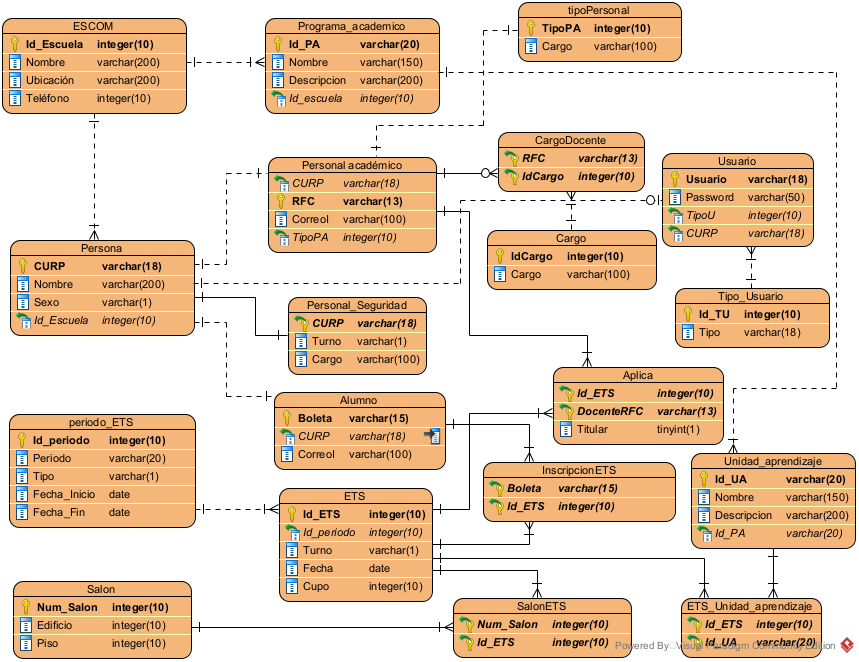
\includegraphics[angle=90,width=.85\textwidth]{images/DER}
		\caption{Modelo del dominio del problema}
		\label{fig:modeloDeDominio}
	\end{center}
\end{figure}

\newpage
%---------------------------------------------------------
\begin{cdtEntidad}{Unidad academica}{Unidad academica}
	\brAttr{Id\_escuela}{Id\_escuela}{Id}{Número de registro usado para identificar a la escuela.}{Sí}
	\brAttr{nombre}{Nombre}{Palabra}
	{Nombre de la escuela}{Sí}
%	\brAttr{ubicacion}{Ubicación}{Frase}
%	{Ubicación en la que se encuentra la escuela.}{Sí}
%	\brAttr{telefono}{Teléfono}{Teléfono}
%	{Teléfono para contactar a la escuela.}{Si}
%- - - - - - - - - - - - - - - - - - - - - - - - - - - - - 
	% \brRelComposition \brRelAgregation
%	\cdtEntityRelSection
%	\brRel{}{Programa\_académico}{ \hyperlink{Unidad academica}{Unidad académica} está compuesto por un \hyperlink{PA}{Programa académico}}	
%	\brRel{}{Persona}{Una \hyperlink{Persona}{Persona} pertenece a \hyperlink{Unidad academica}{Unidad academica}}	
\end{cdtEntidad}
%---------------------------------------------------------
\begin{cdtEntidad}{EscuelaPrograma}{Escuela\_Programa}
	\brAttr{Id\_Escuela}{Id\_Escuela}{Id}{Número de registro usado para identificar a la escuela.}{Sí}
	\brAttr{Id\_PA}{Id\_PA}{Id}
	{Identificación del programa académico que imparte la Unidad académica.}{Sí}
\end{cdtEntidad}
%---------------------------------------------------------
\begin{cdtEntidad}{PA}{Programa\_academico}
	\brAttr{Id\_PA}{Id\_PA}{Id}{Número de registro usado para identificar al programa académico.}{Sí}
	\brAttr{nombre}{Nombre}{Palabra}
	{Nombre del programa académico}{Sí}
	\brAttr{descripcion}{Descripción}{Frase}
	{Descripción que habla sobre el programa académico.}{Sí}
%- - - - - - - - - - - - - - - - - - - - - - - - - - - - -
%	\cdtEntityRelSection
%	\brRel{}{Unidad\_aprendizaje}{Un \hyperlink{PA}{Programa academico} está compuesto por una \hyperlink{UA}{Unidad de aprendizaje}}	
%	\brRel{}{Unidad academica}{Una \hyperlink{Unidad academica}{Unidad academica} está compuesta por un \hyperlink{PA}{Programa académico}}	
\end{cdtEntidad}
%---------------------------------------------------------
\begin{cdtEntidad}{Persona}{Persona}
	\brAttr{CURP}{CURP}{Id}{Código usado para identificar a las personas.}{Sí}
	\brAttr{nombre}{Nombre}{Frase corta}
	{Nombre(s) de la persona.}{Sí}
	\brAttr{ApellidoP}{Apellido\_P}{Frase corta}
	{Apellido paterno de la persona.}{Sí}
	\brAttr{ApellidoM}{Apellido\_M}{Frase corta}
	{Apellido materno de la persona.}{Sí}
	\brAttr{sexo}{Sexo}{Caracter}
	{Letra que servirá para identificar el sexo de un alumno ('M' para masculino, 'F' para femenino).}{Sí}
	\brAttr{Id\_escuela}{Id\_escuela}{Id}
	{Id de la escuela a la que pertenece la persona.}{Si}
	%- - - - - - - - - - - - - - - - - - - - - - - - - - - - -
%	\cdtEntityRelSection
%	\brRel{}{Unidad academica}{Una \hyperlink{Persona}{Persona} pertenece a una \hyperlink{Unidad academica}{Unidad academica}}	
%	\brRel{}{Docente}{Una \hyperlink{Persona}{Persona} es un \hyperlink{Docente}{Docente}}	
%	\brRel{}{Personal\_Seguridad}{Una \hyperlink{Persona}{Persona} es un \hyperlink{PS}{Personal de seguridad}}
%	\brRel{}{Alumno}{Una \hyperlink{Persona}{Persona} es un  \hyperlink{Alumno}{Alumno}}
%	\brRel{}{Usuario}{Una \hyperlink{Persona}{Persona} cuenta con un \hyperlink{Usuario}{Usuario}}
\end{cdtEntidad}
%---------------------------------------------------------
\begin{cdtEntidad}{PersonalAcademico}{Personal académico}
	\brAttr{CURP}{CURP}{Id}{Código usado para identificar a las personas.}{Sí}
	\brAttr{RFC}{RFC}{Id}
	{RFC que identifica al personal académico.}{Sí}
	\brAttr{CorreoI}{CorreoI}{Correo}
	{Correo institucional del personal académico.}{Sí}
	\brAttr{TipoPA}{TipoPA}{Id}{Número que identifica que tipo de personal académico es, ya sea, por ejemplo, un docente o personal de gestión escolar.}{Sí}
	%- - - - - - - - - - - - - - - - - - - - - - - - - - - - -
%	\cdtEntityRelSection
%	\brRel{}{CargoDocente}{Un \hyperlink{PersonalAcademico}{personal académico} puede ser un \hyperlink{CargoDocente}{Docente}}
%	\brRel{}{ETS}{Un \hyperlink{PersonalAcademico}{Docente} \hyperlink{Aplica}{Aplica} un \hyperlink{ETS}{ETS}}
%	\brRel{}{Persona}{Un \hyperlink{PersonalAcademico}{personal académico} es una \hyperlink{Persona}{Persona}}
%	\brRel{}{tipoPersonal}{Un \hyperlink{PersonalAcademico}{personal académico} tiene asignado un \hyperlink{Cargo}{Cargo}}
\end{cdtEntidad}
%---------------------------------------------------------
\begin{cdtEntidad}{tipoPA}{tipoPersonal}
	\brAttr{TipoPA}{TipoPA}{Id}
	{Número que identifica que tipo de personal académico es la persona.}{Sí}
	\brAttr{Cargo}{Cargo}{Frase corta}{Nombre del tipo de personal académico que tendrá la persona.}{Sí}
\end{cdtEntidad}
%---------------------------------------------------------
\begin{cdtEntidad}{CargoDocente}{CargoDocente}
	\brAttr{RFC}{RFC}{Id}
	{RFC que identifica al Docente.}{Sí}
	\brAttr{IdCargo}{IdCargo}{Id}{Código usado para identificar un cargo dentro de la escuela.}{Sí}
\end{cdtEntidad}
%---------------------------------------------------------
\begin{cdtEntidad}{Cargo}{Cargo}
	\brAttr{IdCargo}{IdCargo}{Id}{Código usado para identificar un cargo dentro de la escuela.}{Sí}
	\brAttr{Cargo}{Cargo}{Frase corta}
	{Nombre del cargo existente dentro de la institución escolar.}{Sí}
	%- - - - - - - - - - - - - - - - - - - - - - - - - - - - -
%	\cdtEntityRelSection
%	\brRel{}{CargoDocente}{Un \hyperlink{Cargo}{Cargo} es asignado a un \hyperlink{PersonalAcademico}{Docente}}
\end{cdtEntidad}
%---------------------------------------------------------
\begin{cdtEntidad}{PS}{Personal\_Seguridad}
	\brAttr{CURP}{CURP}{Id}{Código usado para identificar a las personas.}{Sí}
	\brAttr{Turno}{Turno}{Caracter}
	{Letra usada identificar el turno en el que se aplica el ETS ('M' para matutino, 'V' para vespertino).}{Sí}
	\brAttr{Cargo}{Cargo}{Frase corta}
	{Nombre del cargo del personal de seguridad.}{Sí}
	%- - - - - - - - - - - - - - - - - - - - - - - - - - - - -
	\cdtEntityRelSection
	\brRel{}{Persona}{Un \hyperlink{PS}{Personal de seguridad} es una \hyperlink{Persona}{Persona}}
\end{cdtEntidad}
%---------------------------------------------------------
\begin{cdtEntidad}{CargoPS}{CargoPS}
	\brAttr{Id\_Cargo}{Id\_Cargo}{Id}{Código usado para identificar el cargo que tiene el personal de seguridad.}{Sí}
	\brAttr{Nombre}{Nombre}{Frase corta}
	{Nombre del cargo del personal de seguridad.}{Sí}
	\brAttr{Cargo}{Cargo}{Frase corta}
	{Nombre del cargo del personal de seguridad.}{Sí}
\end{cdtEntidad}
%---------------------------------------------------------
\begin{cdtEntidad}{Alumno}{Alumno}
	\brAttr{Boleta}{Boleta}{Id}
	{Código usado para identificar al alumnado de la institución}{Sí}
	\brAttr{CURP}{CURP}{Id}{Código usado para identificar a las personas.}{Sí}
	\brAttr{CorreoI}{CorreoI}{Correo}
	{Correo institucional del alumno.}{Sí}
	\brAttr{Id\_PA}{Id\_PA}{Id}
	{Identificación del programa académico al que pertenece el alumno.}{Sí}
	%- - - - - - - - - - - - - - - - - - - - - - - - - - - - -
%	\cdtEntityRelSection
%	\brRel{}{Persona}{Un \hyperlink{Alumno}{Alumno} es una \hyperlink{Persona}{Persona}}
%	\brRel{}{ETS}{Un \hyperlink{Alumno}{Alumno} tiene una \hyperlink{InscripcionETS}{inscripción} a un \hyperlink{ETS}{ETS}}
\end{cdtEntidad}
%---------------------------------------------------------
\begin{cdtEntidad}{Usuario}{Usuario}
	\brAttr{Usuario}{Usuario}{Usuario}{Nombre de usuario asignado a una persona dentro del sistema.}{Sí}
	\brAttr{Password}{Password}{Contraseña}
	{Contraseña ligada al usuario de una persona registrada dentro del sistema.}{Sí}
	\brAttr{TipoU}{TipoU}{Id}
	{Número que identificará a los tipos de usuario registrados dentro del sistema.}{Sí}
	\brAttr{CURP}{CURP}{Id}
	{Código usado para identificar a las personas.}{Sí}
	%- - - - - - - - - - - - - - - - - - - - - - - - - - - - -
%	\cdtEntityRelSection
%	\brRel{}{Persona}{Un \hyperlink{Usuario}{Usuario} es asignado a una \hyperlink{Persona}{Persona}}
%	\brRel{}{Tipo\_Usuario}{Un \hyperlink{Usuario}{Usuario} tiene un \hyperlink{TU}{Tipo de usuario}}
\end{cdtEntidad}
%---------------------------------------------------------
\begin{cdtEntidad}{TU}{Tipo\_Usuario}
	\brAttr{Id\_TU}{Id\_TU}{Id}
	{RFC que identifica al personal académico.}{Sí}
	\brAttr{Tipo}{Tipo}{Frase corta}{Frase que definirá el tipo de usuario que tienen las personas.}{Sí}
\end{cdtEntidad}
%---------------------------------------------------------
\begin{cdtEntidad}{ETS}{ETS}
	\brAttr{Id\_ETS}{Id\_ETS}{Id}{Número usado para identificar los diferentes ETS registrados.}{Sí}
	\brAttr{Id\_periodo}{Id\_periodo}{Id}
	{Número usado para identificar el periodo en el que se realiza el ETS.}{Sí}
	\brAttr{Turno}{Turno}{Caracter}
	{Letra usada identificar el turno en el que se aplica el ETS ('M' para matutino, 'V' para vespertino).}{Sí}
	\brAttr{Fecha}{Fecha}{Fecha}
	{Fecha y hora en la que se realizará el ETS.}{Sí}
	\brAttr{Cupo}{Cupo}{Número}
	{Número de personas permitidas a realizar el ETS.}{Sí}
	\brAttr{Id\_UA}{Id\_UA}{Número}
	{Identificación de la Unidad de aprendizaje del ETS.}{Sí}
	\brAttr{Duracion}{Duracion}{Número}
	{Duración en horas del ETS.}{Sí}
	%- - - - - - - - - - - - - - - - - - - - - - - - - - - - -
%	\cdtEntityRelSection
%	\brRel{}{periodo\_ETS}{Un \hyperlink{ETS}{ETS} se realiza un en \hyperlink{PETS}{periodo}}
%	\brRel{}{Alumno}{En un \hyperlink{ETS}{ETS} está \hyperlink{InscripcionETS}{inscrito} un \hyperlink{Alumno}{Alumno}}
%	\brRel{}{Personal academico}{Un \hyperlink{ETS}{ETS} es \hyperlink{Aplica}{aplicado} por un \hyperlink{PersonalAcademico}{Docente}}
%	\brRel{}{Salon}{A un \hyperlink{ETS}{ETS} le \hyperlink{SalonETS}{corresponde} un \hyperlink{Salon}{Salón}}
%	\brRel{}{Unidad\_Aprendizaje}{Un \hyperlink{ETS}{ETS} \hyperlink{ETSUA}{es de} una \hyperlink{UA}{Unidad de Aprendizaje}.}
\end{cdtEntidad}
%---------------------------------------------------------
\begin{cdtEntidad}{PETS}{periodo\_ETS}
	\brAttr{Id\_periodo}{Id\_periodo}{Id}{Número usado para identificar el periodo en el que se realizarán los ETS registrados.}{Sí}
	\brAttr{Periodo}{Periodo}{Cadena de texto corta}
	{Periodo registrado en el que se realizarán los ETS.}{Sí}
	\brAttr{Tipo}{Tipo}{Caracter}
	{Letra usada identificar el tipo de los ETS que se aplicarán ('O' para ordinario, 'E' para especial).}{Sí}
	\brAttr{Fecha\_Inicio}{Fecha\_Inicio}{Fecha}
	{Fecha en la que iniciará el periodo de los ETS.}{Sí}
	\brAttr{Fecha\_Fin}{Fecha\_Fin}{Fecha}
	{Fecha en la que terminará el periodo de los ETS.}{Sí}
	%- - - - - - - - - - - - - - - - - - - - - - - - - - - - -
%	\cdtEntityRelSection
%	\brRel{}{ETS}{En un \hyperlink{PETS}{periodo de ETS} se realizan los \hyperlink{ETS}{ETS}.}
\end{cdtEntidad}
%---------------------------------------------------------
\begin{cdtEntidad}{Aplica}{Aplica}
	\brAttr{Id\_ETS}{Id\_ETS}{Id}{Número usado para identificar los diferentes ETS registrados.}{Sí}
	\brAttr{DocenteRFC}{DocenteRFC}{Id}
	{RFC que identifica al Docente.}{Sí}
	\brAttr{Titular}{Titular}{Booleano}
	{Booleano que identificará si el profesor que aplicará el ETS es el titular o es un ayudante.}{Sí}
\end{cdtEntidad}
%---------------------------------------------------------
\begin{cdtEntidad}{InscripcionETS}{InscripcionETS}
	\brAttr{Boleta}{Boleta}{Id}
	{Código usado para identificar al alumnado de la institución}{Sí}
	\brAttr{Id\_ETS}{Id\_ETS}{Id}{Número usado para identificar los diferentes ETS registrados.}{Sí}
\end{cdtEntidad}
%---------------------------------------------------------
\begin{cdtEntidad}{SalonETS}{SalonETS}
	\brAttr{Num\_Salon}{Num\_Salon}{Id}
	{Número usado para identificar al salón en el que se aplicará un ETS.}{Sí}
	\brAttr{Id\_ETS}{Id\_ETS}{Id}{Número usado para identificar los diferentes ETS registrados.}{Sí}
\end{cdtEntidad}
%---------------------------------------------------------
\begin{cdtEntidad}{Salon}{Salon}
	\brAttr{Num\_Salon}{Num\_Salon}{Id}
	{Número usado para identificar el salón en el que se aplicará un ETS.}{Sí}
	\brAttr{Edificio}{Edificio}{Número}
	{Número usado para identificar el edificio en el que se realizará el ETS.}{Sí}
	\brAttr{Piso}{Piso}{Número}
	{Número usado para identificar el piso del edificio en el que se realizará el ETS.}{Sí}
	\brAttr{TipoSalon}{TipoSalon}{Id}
	{Identificación del tipo de salón en el que se va a aplicar el ETS.}{Sí}
	%- - - - - - - - - - - - - - - - - - - - - - - - - - - - -
%	\cdtEntityRelSection
%	\brRel{}{ETS}{Un \hyperlink{Salon}{Salon} es \hyperlink{SalonETS}{ocupado} para llevar a cabo un \hyperlink{ETS}{ETS}.}
\end{cdtEntidad}
%---------------------------------------------------------
\begin{cdtEntidad}{TipoSalon}{TipoSalon}
	\brAttr{Num\_Salon}{Num\_Salon}{Id}
	{Número usado para identificar el salón en el que se aplicará un ETS.}{Sí}
	\brAttr{Tipo}{Tipo}{Frase corta}
	{Frase indicando el tipo de salón en el que se aplicará el ETS.}{Sí}
	%- - - - - - - - - - - - - - - - - - - - - - - - - - - - -
	%	\cdtEntityRelSection
	%	\brRel{}{ETS}{Un \hyperlink{Salon}{Salon} es \hyperlink{SalonETS}{ocupado} para llevar a cabo un \hyperlink{ETS}{ETS}.}
\end{cdtEntidad}
%---------------------------------------------------------
\begin{cdtEntidad}{UA}{Unidad\_aprendizaje}
	\brAttr{Id\_UA}{Id\_UA}{Id}
	{Identificación de la Unidad de Aprendizaje.}{Sí}
	\brAttr{Nombre}{Nombre}{Número}
	{Número usado para identificar el edificio en el que se realizará el ETS.}{Sí}
	\brAttr{Descripcion}{Descripcion}{Número}
	{Número usado para identificar el piso del edificio en el que se realizará el ETS.}{Sí}
	\brAttr{Id\_PA}{Id\_PA}{Id}
	{Número usado para identificar el piso del edificio en el que se realizará el ETS.}{Sí}
	%- - - - - - - - - - - - - - - - - - - - - - - - - - - - -
	\cdtEntityRelSection
	\brRel{}{ETS}{A una \hyperlink{UA}{Unidad de aprendizaje} le \hyperlink{ETSUA}{corresponde} una serie de \hyperlink{ETS}{ETS}.}
\end{cdtEntidad}
%---------------------------------------------------------
\subsection{Modelado de Reglas de negocio}

\begin{BussinesRule}{RN1}{Acceso al sistema.}
	\BRitem[Tipo:] Acceso. 
	\BRitem[Clase:] Condicional. 
	\BRitem[Nivel:] Estricto.
	\BRitem[Descripción:] El acceso a nuestro sistema será permitido solo para los Empleados y estudiantes de la ESCOM.
	\BRitem[Motivación:] Evitar el acceso no autorizado a otras personas que no sean de la ESCOM..

	\BRitem[Referenciado por:] \hyperlink{CU-01}{CU-01} y \hyperlink{CU41}{CU-41}.
\end{BussinesRule}

\begin{BussinesRule}{RN2}{ Acceso a las funcionalidades del docente.}
    \BRitem[Tipo:] Acceso. 
    \BRitem[Clase:] Condicional. 
    \BRitem[Nivel:] Estricto.
    \BRitem[Descripción:] Los docentes solo podrán acceder y revisar la información de los ETS que tengan asignados.
    \BRitem[Motivación:] Para evitar que los docentes se confundan, accedan a información que no les corresponde o modifiquen información que no les corresponde.

    \BRitem[Referenciado por:] \hyperlink{CU-01}{CU-01} y \hyperlink{CU-04}{CU-04}.
\end{BussinesRule}

\begin{BussinesRule}{RN3}{ Acceso a las funcionalidades del personal de seguridad.}
    \BRitem[Tipo:] Acceso. 
    \BRitem[Clase:] Condicional. 
    \BRitem[Nivel:] Estricto.
    \BRitem[Descripción:] El personal de seguridad solo podrán acceder y revisar la información relacionada con el acceso de los alumnos a la ESCOM de los días en los que se presenten ETS.
    \BRitem[Motivación:] Para evitar que el personal de seguridad se confunda, accedan a información que no les corresponde o modifiquen información que no les corresponde.

    \BRitem[Referenciado por:] \hyperlink{CU-01}{CU-01} y \hyperlink{CU-12}{CU-12}, \hyperlink{CU-13}{CU-13}, \hyperlink{CU-14}{CU-14} y \hyperlink{CU-15}{CU-15}.
\end{BussinesRule}

\begin{BussinesRule}{RN4}{ Acceso a las funcionalidades web}
	\BRitem[Tipo:] Habilitación.
	\BRitem[Clase:] Condicional.
	\BRitem[Nivel:] Estricta.
	\BRitem[Descripción:] El sistema permitirá únicamente a el personal de gestión escolar y al personal la DAE acceder al sistema web.
	\BRitem[Motivación:] Se necesita separar las funcionalidades de los empleados para que el sistema tenga cohesión y para que el sistema web no referencie al sistema movil.
	\BRitem[Referenciado por:] \hyperlink{CU-41}{CU-41}.
	\end{BussinesRule}

\begin{BussinesRule}{RN5} {Consultar periodos del docente}
	\BRitem[Tipo:] Habilitación.
	\BRitem[Clase:] Condicional.
	\BRitem[Nivel:] Estricta.
	\BRitem[Descripción:] El sistema permitirá únicamente a los docentes autenticados consultar los períodos de ETS que tiene asignados.
	\BRitem[Motivación:] Garantizar que solo usuarios autorizados consulten información sensible.			
	\BRitem[Referenciado por:] \hyperlink{CU-04}{CU-04}.
	\end{BussinesRule}

\begin{BussinesRule}{RN6} {Visualizar lista de alumnos inscritos}
	\BRitem[Tipo:] Acceso.
	\BRitem[Clase:] Condicional.
	\BRitem[Nivel:] Estricta.
	\BRitem[Descripción:] El sistema permitirá al docente consultar únicamente la lista de los alumnos inscritos a los ETS que le han sido asignados.
	\BRitem[Motivación:] Permitir que los docentes puedan visualizar la información de los estudiantes inscritos a los ETS que tenga asignados.
	\BRitem[Referenciado por:] \hyperlink{CU-09}{CU-09}.
	\end{BussinesRule}

\begin{BussinesRule}{RN7} {Acceso al asignar remplazo}
    \BRitem[Tipo:] Acceso.
    \BRitem[Clase:] Condicional.
    \BRitem[Nivel:] Estricta.
    \BRitem[Descripción:] El sistema permitirá solo al presidente de academia  y al jefe de departamento consultar la lista de solicitudes de remplazo y posteriormente asignar un remplazo.
    \BRitem[Motivación:] Hacer que solo el personal capacitado y responsable asigne los remplazos a los ETS.
    \BRitem[Referenciado por:] \hyperlink{CU-42}{CU-42}.
    \end{BussinesRule}

\begin{BussinesRule}{RN8} {Cantidad de pruebas de reconocimiento facial}
    \BRitem[Tipo:]Habilitación.
    \BRitem[Clase:]Cronometrada.
    \BRitem[Nivel:] Estricta.
    \BRitem[Descripción:] El alumno solo puede realizar un máximo de 3 pruebas de reconocimiento facial dentro de la aplicación.
    \BRitem[Motivación:] Evitar que el alumno le pida a alguien más que  pruebe constantemente el reconocimiento facial hasta que se parezca a el/ella.
    \BRitem[Referenciado por:] \hyperlink{CU-19}{CU-19}.
    \end{BussinesRule}

\begin{BussinesRule}{RN9} {Cantidad de intentos fallidos de inicio de sesión}
    \BRitem[Tipo:]Habilitación.
    \BRitem[Clase:] Cronometrada.
    \BRitem[Nivel:] Estricta.
    \BRitem[Descripción:] El sistema permitirá solo a todos los usuarios un máximo de 5 intentos de inicio de sesión fallidos antes de bloquear la cuenta del usuario.
    \BRitem[Motivación:] Asegurar la seguridad de los usuarios y evitar que personas no autorizadas entren al sistema.
    \BRitem[Referenciado por:] \hyperlink{CU-01}{CU-01}, y \hyperlink{CU-41}{CU-41}.
    \end{BussinesRule}

\begin{BussinesRule}{RN10} {Acceso a solo la información de los ETS }
    \BRitem[Tipo:]Habilitadora.
    \BRitem[Clase:]Condicional.
    \BRitem[Nivel:] Estricta.
    \BRitem[Descripción:] El sistema permitirá que los alumnos puedan ingresar solo a la información de sus ETS inscritos y solo consultar a la información (no podrán modificarla).
    \BRitem[Motivación:] Evitar que los alumnos cambien la información de los ETS y evitar que los alumnos sepan de otros alumnos que presentaran el mismo ETS (esto para no fomentar la formación de acuerdos entre los alumnos).
    \BRitem[Referenciado por:] \hyperlink{CU-19}{CU-19}.
    \end{BussinesRule}

% Alfredo

\begin{BussinesRule}{BR11}{Registro de usuarios válidos.} 
    \BRitem[Tipo:] Habilitadora
    \BRitem[Clase:] Integridad
    \BRitem[Nivel:] Estricta
    \BRitem[Descripción:] Todos los usuarios registrados dentro del sistema deberán de estar registrados dentro de la tabla “Persona”. 
    \BRitem[Motivación:] Asegurar que solo la comunidad de la institución pueda acceder a la escuela. 
    \BRitem[Referenciado por:] \hyperlink{Usuario}{Usuario} 
    \end{BussinesRule}

\begin{BussinesRule}{BR12}{Registro de personal académico.} 
    \BRitem[Tipo:] Habilitadora
    \BRitem[Clase:] Condición.
    \BRitem[Nivel:] Estricta
    \BRitem[Descripción:] Para registrar al personal académico se deberá de dar de alta un RFC, un correo institucional válido y especificar el cargo que tiene dentro de la institución. Este puede variar entre un docente o personal administrativo, como lo es el personal de gestión escolar. En caso de ser un docente se debe especificar su cargo dentro de la escuela, como lo es el jefe de academia, presidente de academia, director o subdirector. 
    \BRitem[Motivación:] Moderar los diferentes permisos de los usuarios dependiendo del cargo que tengan dentro de la escuela. 
    \BRitem[Referenciado por:] \hyperlink{PersonalAcademico}{Personal Académico} 
    \end{BussinesRule}

\begin{BussinesRule}{BR13}{Límite de alumnos en un ETS.} 
    \BRitem[Tipo:] Cronometrada. 
    \BRitem[Clase:] Condición.
    \BRitem[Nivel:] Estricta
    \BRitem[Descripción:] Un alumno se podrá inscribir a un ETS únicamente si la cantidad de alumnos aún no excede el cupo límite de un ETS.
    \BRitem[Motivación:] Evitar el sobrecupo de un salón el día del ETS.
    \BRitem[Referenciado por:] \hyperlink{ETS}{ETS} 
    \end{BussinesRule}
    
\begin{BussinesRule}{BR14}{Fecha de aplicación de los ETS.} 
    \BRitem[Tipo:] Cronometrada. 
    \BRitem[Clase:] Condición.
    \BRitem[Nivel:] Estricta
    \BRitem[Descripción:] Las fechas de los ETS deben de estar dentro del periodo especificado del mismo, en caso contrario no se podrá dar de alta. 
    \BRitem[Motivación:] Tener un control sobre las fechas en las que se aplican los ETS. 
    \BRitem[Referenciado por:] \hyperlink{ETS}{ETS} 
    \end{BussinesRule}

\begin{BussinesRule}{BR15}{Registro de un ETS} 
    \BRitem[Tipo:] Habilitadora. 
    \BRitem[Clase:] Condición.
    \BRitem[Nivel:] Estricta
    \BRitem[Descripción:] Los ETS deberán de especificar siempre el turno en el ques e van a aplicar, especificar el periodo en el que se aplican y el cupo que se tendrá para ese ETS.
    \BRitem[Motivación:] Tener un mejor control sobre la información de los ETS.
    \BRitem[Referenciado por:] \hyperlink{ETS}{ETS} 
    \end{BussinesRule}

\begin{BussinesRule}{BR16}{Asignación de salón para un ETS} 
    \BRitem[Tipo:] Habilitadora. 
    \BRitem[Clase:] Condición	.
    \BRitem[Nivel:] Estricta
    \BRitem[Descripción:] Un salón solo puede ser asignado a un ETS si no ha sido asignado para otro ETS.
    \BRitem[Motivación:] Evitar la sobreasignación de salones.
    \BRitem[Referenciado por:] \hyperlink{SalonETS}{Salón del ETS} 
    \end{BussinesRule}

\begin{BussinesRule}{BR17}{Permisos del usuario de los docentes.} 
    \BRitem[Tipo:] Ejecutiva.
    \BRitem[Clase:] Autorización.
    \BRitem[Nivel:] Estricta
    \BRitem[Descripción:] Si un docente tiene asignado más de un cargo dentro de la institución, el sistema le mostrará las interfaces correspondientes a cada uno de los cargos. El acceso a las interfaces dependerá de las funcionalidades permitidas por cada cargo.
    \BRitem[Motivación:] Asegurar que los docentes tengan acceso a todas las funciones dependiendo del cargo que tengan.
    \BRitem[Referenciado por:] \hyperlink{CargoDocente}{Cargo del docente} 
    \end{BussinesRule}

\begin{BussinesRule}{BR18}{Número de docentes aplicadores de un ETS.} 
    \BRitem[Tipo:] Habilitadora. 
    \BRitem[Clase:] Condición.
    \BRitem[Nivel:] Estricta
    \BRitem[Descripción:] Un mismo ETS puede ser aplicado por múltiples docentes en diferentes salones.
    \BRitem[Motivación:] Asegurar que todos los ETS tengan por lo menos un aplicador, ya sea en uno o más salones.
    \BRitem[Referenciado por:] \hyperlink{Aplica}{Tabla Aplica} 
    \end{BussinesRule}

\begin{BussinesRule}{BR19}{Inscripción de un ETS.} 
    \BRitem[Tipo:] Habilitadora. 
    \BRitem[Clase:] Autorización.
    \BRitem[Nivel:] Estricta
    \BRitem[Descripción:] Un alumno no puede estar inscrito en dos ETS que se lleven a cabo en el mismo horario.
    \BRitem[Motivación:] Evitar el solapamiento de dos o más ETS.
    \BRitem[Referenciado por:] \hyperlink{InscripcionETS}{Inscripción de un ETS} 
    \end{BussinesRule}

\begin{BussinesRule}{BR20}{Aplicador titular de un ETS.} 
    \BRitem[Tipo:] Integridad
    \BRitem[Clase:] Cronometrada.
    \BRitem[Nivel:] Estricta
    \BRitem[Descripción:] Los ETS deberán contar siempre con un docente titular que es el docente principal que va a aplicar el ETS. En caso de sustitución del docente o apoyo a este, también se especificará que estos son ayudantes y no titulares.
    \BRitem[Motivación:] Garantizar la asignación de roles dentro del sistema.
    \BRitem[Referenciado por:] \hyperlink{Aplica}{Tabla Aplica} 
    \end{BussinesRule}
    

%
\begin{BussinesRule}{RN21} {Acceso a información sobre el acceso a los ETS}
    \BRitem[Tipo:] Acceso.
    \BRitem[Clase:]Condicional.
    \BRitem[Nivel:] Estricta.
    \BRitem[Descripción:] El sistema permitirá que solo los alumnos puedan acceder a la información sobre los ETS en una pantalla.
    \BRitem[Motivación:] Permitir que los alumnos conozcan el proceso de acceso a los ETS y evitar confusiones y malentendidos.
    \BRitem[Referenciado por:] \hyperlink{CU-20}{CU-20}.
    \end{BussinesRule}

\begin{BussinesRule}{RN22} {Estructura de la CURP}
    \BRitem[Tipo:]Integridad.
    \BRitem[Clase:]Condicional.
    \BRitem[Nivel:] Estricta.
    \BRitem[Descripción:] La CURP debe de tener exactamente 18 caracteres y debe de poseer solo letras y números.
    \BRitem[Motivación:] Para mantener la estructura correcta de la CURP y evitar que se Introduzca datos inválidos.
    \BRitem[Referenciado por:] \hyperlink{CU-21}{CU-21}, \hyperlink{CU-22}{CU-22}, \hyperlink{CU-33}{CU-33} y \hyperlink{CU-37}{CU-37}.
    \end{BussinesRule}

\begin{BussinesRule}{RN23} {Estructura de la Boleta}
    \BRitem[Tipo:]Integridad.
    \BRitem[Clase:]Condicional.
    \BRitem[Nivel:] Estricta.
    \BRitem[Descripción:] La Boleta debe de tener exactamente 10 caracteres y debe de poseer solo números.
    \BRitem[Motivación:] Para mantener la estructura correcta de la Boleta y evitar que se Introduzca datos inválidos.
    \BRitem[Referenciado por:] \hyperlink{CU-21}{CU-21}, \hyperlink{CU-22}{CU-22}, \hyperlink{CU-33}{CU-33} y \hyperlink{CU-37}{CU-37}.
    \end{BussinesRule}

\begin{BussinesRule}{RN24} {Estructura del correo institucional del alumno}
    \BRitem[Tipo:]Integridad.
    \BRitem[Clase:]Condicional.
    \BRitem[Nivel:] Estricta.
    \BRitem[Descripción:] El correo institucional del alumno debe de seguir la estructura [texto][@][alumno.ipn.mx]
    \BRitem[Motivación:] Para mantener la estructura correcta del correo institucional y evitar que se Introduzca datos inválidos.
    \BRitem[Referenciado por:] \hyperlink{CU-21}{CU-21} y \hyperlink{CU-22}{CU-22}.
    \end{BussinesRule}

\begin{BussinesRule}{RN25} {Cantidad de alumnos por salud}
    \BRitem[Tipo:] Habilitación.
    \BRitem[Clase:] Cronometrada.
    \BRitem[Nivel:] Estricta.
    \BRitem[Descripción:] Los salones tienen un cupo máximo de 30 alumnos.
    \BRitem[Motivación:] Para evitar aglomeraciones de alumnos durante un ETS.
    \BRitem[Referenciado por:] \hyperlink{CU-21}{CU-21} y \hyperlink{CU-22}{CU-22}.
    \end{BussinesRule}

\begin{BussinesRule}{RN26} {Asignación de salones}
    \BRitem[Tipo:] Habilitación.
    \BRitem[Clase:] Cronometrada.
    \BRitem[Nivel:] Estricta.
    \BRitem[Descripción:] Los salones solo pueden ser asignados a un ETS durante un periodo de ETS concreto.
    \BRitem[Motivación:] Para evitar que los salones sean asignados a 2 o más ETS distintos a la vez.
    \BRitem[Referenciado por:] \hyperlink{CU-25}{CU-25}.
    \end{BussinesRule}

\begin{BussinesRule}{RN27} {Estructura del dato salón}
    \BRitem[Tipo:] Integridad.
    \BRitem[Clase:]Condicional.
    \BRitem[Nivel:] Estricta.
    \BRitem[Descripción:] El dato salón está conformado por 4 números de los cuales el primer indica el edificio, el segundo el piso y los otros dos el número del salón .
    \BRitem[Motivación:] Para mantener la estructura correcta del dato salón y evitar que se Introduzca datos inválidos.
    \BRitem[Referenciado por:] \hyperlink{CU-29}{CU-29}.
    \end{BussinesRule}

\begin{BussinesRule}{RN28} {Valores del turno }
    \BRitem[Tipo:]Integridad.
    \BRitem[Clase:]Condicional.
    \BRitem[Nivel:] Estricta.
    \BRitem[Descripción:] El turno solo puede ser matutino o vespertino.
    \BRitem[Motivación:] Para establecer que los ETS no se pueden hacer en periodos de tiempo irregulares.
    \BRitem[Referenciado por:] \hyperlink{CU-29}{CU-29} y \hyperlink{CU-33}{CU-33}.
    \end{BussinesRule}

\begin{BussinesRule}{RN29} {Fecha del ETS}
    \BRitem[Tipo:]Integridad.
    \BRitem[Clase:]Condicional.
    \BRitem[Nivel:] Estricta.
    \BRitem[Descripción:] La fecha del del ETS solo puede ser un día que este dentro del periodo del ETS asignado.
    \BRitem[Motivación:] Para establecer que los ETS no pueden estar fuera de la fecha del periodo de ETS asignado.
    \BRitem[Referenciado por:] \hyperlink{CU-29}{CU-29}.
    \end{BussinesRule}

\begin{BussinesRule}{RN30} {Selección de periodo de ETS para el ETS actual}
    \BRitem[Tipo:]Integridad.
    \BRitem[Clase:]Condicional.
    \BRitem[Nivel:] Estricta.
    \BRitem[Descripción:] Para dar de alta un ETS solo se puede poner el periodo de ETS actual o el más próximo si no hay actual.
    \BRitem[Motivación:] Para no asignar ETS en fechas imposibles.
    \BRitem[Referenciado por:] \hyperlink{CU-29}{CU-29}.
    \end{BussinesRule}


\begin{BussinesRule}{RN31} {Valores del tipo de periodo de ETS}
    \BRitem[Tipo:]Integridad.
    \BRitem[Clase:]Condicional.
    \BRitem[Nivel:] Estricta.
    \BRitem[Descripción:] El tipo del ETS solo puede ser ordinario o extraordinario.
    \BRitem[Motivación:] Para establecer correctamente los 2 tipos de ETS.
    \BRitem[Referenciado por:] \hyperlink{CU-25}{CU-25}.
    \end{BussinesRule}

\begin{BussinesRule}{RN32} {Asignación de fechas al periodo de ETS}
    \BRitem[Tipo:]Integridad.
    \BRitem[Clase:]Condicional.
    \BRitem[Nivel:] Estricta.
    \BRitem[Descripción:] Las fechas de inicio y de fin deben de ser validas.
    \BRitem[Motivación:] Para evitar asignar fechas de ETS imposibles.
    \BRitem[Referenciado por:] \hyperlink{CU-25}{CU-25}.
    \end{BussinesRule}

\begin{BussinesRule}{RN33} {Asignación de unidad de aprendizaje}
    \BRitem[Tipo:]Integridad.
    \BRitem[Clase:]Condicional.
    \BRitem[Nivel:] Estricta.
    \BRitem[Descripción:] La unidad de aprendizaje debe de estar registrada en el sistema.
    \BRitem[Motivación:] Para evitar asignar unidad de aprendizaje falsas.
    \BRitem[Referenciado por:] \hyperlink{CU-29}{CU-29}.
    \end{BussinesRule}

\begin{BussinesRule}{RN34} {Asignar sexo }
    \BRitem[Tipo:]Integridad.
    \BRitem[Clase:]Condicional.
    \BRitem[Nivel:] Estricta.
    \BRitem[Descripción:] El sexo de los usuarios se refiero al sexo biológico y no al género por lo que solo puede tomar el valor de masculino o femenino.
    \BRitem[Motivación:] Evitar confusiones y simplificar los daros guardados en la base de datos.
    \BRitem[Referenciado por:] \hyperlink{CU-21}{CU-21}, \hyperlink{CU-22}{CU-22}, \hyperlink{CU-33}{CU-33} y \hyperlink{CU-37}{CU-37}.
    \end{BussinesRule}

\begin{BussinesRule}{RN35} {Cantidad de fotos tomadas en la credencialización }
    \BRitem[Tipo:]Integridad.
    \BRitem[Clase:]Condicional.
    \BRitem[Nivel:] Estricta.
    \BRitem[Descripción:] Para la credencialización se tomaran 5 fotos.
    \BRitem[Motivación:] Para obtener datos para el entrenamiento de la red neuronal.
    \BRitem[Referenciado por:] \hyperlink{CU-22}{CU-22} y \hyperlink{CU-23}{CU-23}.
    \end{BussinesRule}

\begin{BussinesRule}{RN36} {Visualización del calendario escolar.}
    \BRitem[Tipo:] Acceso.
    \BRitem[Clase:] Condicional.
    \BRitem[Nivel:] Estricta.
    \BRitem[Descripción:] El sistema permitirá a los usuarios visualizar el calendario escolar completo, incluyendo las fechas programadas para los periodos de ETS.
    \BRitem[Motivación:] Permitir que los usuarios tengan acceso a la información actualizada del calendario escolar.
    \BRitem[Referenciado por:] \hyperlink{CU-02}{CU-02}.
    \end{BussinesRule}

\begin{BussinesRule}{RN37}{Actualizar del calendario escolar.}
    \BRitem[Tipo:] Habilitación.
    \BRitem[Clase:] Condicional.
    \BRitem[Nivel:] Estricta.
    \BRitem[Descripción:] El calendario escolar debe ser actualizado para reflejar cambios administrativos, y el sistema debe sincronizar esta información de manera automática.
    \BRitem[Motivación:] Asegurar que los usuarios tengan acceso a la información actualizada.
    \BRitem[Referenciado por:] \hyperlink{CU-02}{CU-02}.
    \end{BussinesRule}

\begin{BussinesRule}{RN38}{Visualizar de notificaciones.}
    \BRitem[Tipo:] Acceso.
    \BRitem[Clase:] Condicional.
    \BRitem[Nivel:] Estricta.
    \BRitem[Descripción:] El sistema permitirá a los usuarios revisar sus notificaciones.
    \BRitem[Motivación:] Permitir que los usuarios puedan visualizar las notificaciones de manera fácil.
    \BRitem[Referenciado por:] \hyperlink{CU-03}{CU-03}.
    \end{BussinesRule}

\begin{BussinesRule}{RN39}{Marcar de notificaciones como leídas.}
    \BRitem[Tipo:] Habilitación.
    \BRitem[Clase:] Condicional.
    \BRitem[Nivel:] Estricta.
    \BRitem[Descripción:] El sistema permitirá a los usuarios marcar una notificación como leída una vez que la hayan revisado.
    \BRitem[Motivación:] Facilitar la organización de las notificaciones.
    \BRitem[Referenciado por:] \hyperlink{CU-03}{CU-03}.
    \end{BussinesRule}

\begin{BussinesRule}{RN40}{Ordenar notificaciones.}
    \BRitem[Tipo:] Habilitación.
    \BRitem[Clase:] Condicional.
    \BRitem[Nivel:] Estricta.
    \BRitem[Descripción:] Las notificaciones deberán mostrarse ordenadas por fecha, de la más reciente a la más antigua.
    \BRitem[Motivación:] Mejorar la experiencia del usuario al priorizar las notificaciones más relevantes.
    \BRitem[Referenciado por:] \hyperlink{CU-03}{CU-03}.
    \end{BussinesRule}

\begin{BussinesRule}{RN41}{Consultar información de los ETS asignados.}
    \BRitem[Tipo:] Acceso.
    \BRitem[Clase:] Condicional.
    \BRitem[Nivel:] Estricta.
    \BRitem[Descripción:] El sistema debe permitir al docente visualizar la información de los ETS que le han sido asignados.
    \BRitem[Motivación:] Permitir que los docentes tengan acceso a la información de sus ETS asignados. 
    \BRitem[Referenciado por:] \hyperlink{CU-06}{CU-06}.
    \end{BussinesRule}

\begin{BussinesRule}{RN42}{Mostrar la información actualizada de los ETS.}
    \BRitem[Tipo:] Acceso.
    \BRitem[Clase:] Ejecutiva.
    \BRitem[Nivel:] Estricta.
    \BRitem[Descripción:] La información mostrada debe estar actualizada y reflejar cualquier cambio administrativo relacionado con los ETS asignados.
    \BRitem[Motivación:] Evitar inconsistencias en la información presentada al docente.
    \BRitem[Referenciado por:] \hyperlink{CU-06}{CU-06}.
    \end{BussinesRule}

\begin{BussinesRule}{RN43}{Filtrar los ETS por docente.}
    \BRitem[Tipo:] Acceso.
    \BRitem[Clase:] Condicional.
    \BRitem[Nivel:] Estricta.
    \BRitem[Descripción:] La información de los ETS asignados debe estar filtrada para que cada docente solo pueda visualizar los ETS que le correspondan.
    \BRitem[Motivación:] Proteger la privacidad de la información de otros docentes.
    \BRitem[Referenciado por:] \hyperlink{CU-06}{CU-06}.
    \end{BussinesRule}

\begin{BussinesRule}{RN44}{Visualizar la lista de alumnos inscritos.}
    \BRitem[Tipo:] Acceso.
    \BRitem[Clase:] Condicional.
    \BRitem[Nivel:] Estricta.
    \BRitem[Descripción:] El sistema permitirá al docente consultar la lista completa de los alumnos inscritos a un ETS asignado.
    \BRitem[Motivación:] Permitir al docente consultar la lista de alumnos inscritos que van a presentar un ETS que tenga asignado.
    \BRitem[Referenciado por:] \hyperlink{CU-08}{CU-08}.
    \end{BussinesRule}

\begin{BussinesRule}{RN45}{Mostrar información de alumnos.}
    \BRitem[Tipo:] Acceso.
    \BRitem[Clase:] Condicional.
    \BRitem[Nivel:] Estricta.
    \BRitem[Descripción:] La lista debe incluir información de los alumnos como Boleta, nombre completo y fotografía.
    \BRitem[Motivación:] Facilitar al docente la identificación de los alumnos durante el ETS.
    \BRitem[Referenciado por:] \hyperlink{CU-08}{CU-08}.
    \end{BussinesRule}

\begin{BussinesRule}{RN46}{Tomar asistencia de los alumnos inscritos a ETS.}
    \BRitem[Tipo:] Acceso.
    \BRitem[Clase:] Condicional.
    \BRitem[Nivel:] Estricta.
    \BRitem[Descripción:] El sistema permitirá al docente registrar la asistencia de los alumnos inscritos al ETS asignado.
    \BRitem[Motivación:] Garantizar que la asistencia solo sea tomada para los alumnos que están inscritos en el ETS.
    \BRitem[Referenciado por:] \hyperlink{CU-09}{CU-09}.
    \end{BussinesRule}

\begin{BussinesRule}{RN47}{Analizar la identidad del alumno.}
    \BRitem[Tipo:] Acceso.
    \BRitem[Clase:] Condicional.
    \BRitem[Nivel:] Estricta.
    \BRitem[Descripción:] El sistema deberá analizar el rostro de cada alumno y proporcionar un indicador comparando las características registradas y las detectadas por el reconocimiento facial.
    \BRitem[Motivación:] Facilitar el proceso pase de lista al docente. 
    \BRitem[Referenciado por:] \hyperlink{CU-09}{CU-09}.
    \end{BussinesRule}

\begin{BussinesRule}{RN48}{Mostrar la lista de asistencia de los alumnos.}
    \BRitem[Tipo:] Acceso.
    \BRitem[Clase:] Condicional.
    \BRitem[Nivel:] Estricta.
    \BRitem[Descripción:] El sistema permitirá al docente visualizar el estatus del pase de lista.
    \BRitem[Motivación:] Consultar los datos registrados previamente en el pase de lista.
    \BRitem[Referenciado por:] \hyperlink{CU-10}{CU-10}.
    \end{BussinesRule}

\begin{BussinesRule}{RN49}{Acceso autorizado para visualizar la información del alumno}
    \BRitem[Tipo:] Acceso.
    \BRitem[Clase:] Condicional.
    \BRitem[Nivel:] Estricta.
    \BRitem[Descripción:] El sistema permitirá a los docentes visualizar la información y foto de un alumno únicamente si tienen permisos autorizados.
    \BRitem[Motivación:] Garantizar que solo los docentes con autorización puedan consultar datos de los alumnos.
    \BRitem[Referenciado por:] \hyperlink{CU-11}{CU-11}.
    \end{BussinesRule}

\begin{BussinesRule}{RN50}{Privacidad de los datos de los alumnos.}
    \BRitem[Tipo:] .
    \BRitem[Clase:] Condicional.
    \BRitem[Nivel:] Estricta.
    \BRitem[Descripción:] La información y foto del alumno no podrán ser compartidas ni divulgadas sin el consentimiento del alumno.
    \BRitem[Motivación:] Proteger la privacidad y confidencialidad de los datos personales de los alumnos.
    \BRitem[Referenciado por:] \hyperlink{CU-11}{CU-11}.
    \end{BussinesRule}

\begin{BussinesRule}{RN51}{Validación de la credencial escolar.}
    \BRitem[Tipo:] Acceso, habilitacion o integridad
    \BRitem[Clase:] Condicional, Cronometrada o ejecutiva 
    \BRitem[Nivel:] Estricta.
    \BRitem[Descripción:] El sistema permitirá al personal de seguridad consultar la información de un alumno únicamente si se escanea correctamente el código QR de su credencial.
    \BRitem[Motivación:] Permitir que la información del alumno solo sea accesible por persona autorizado.
    \BRitem[Referenciado por:] \hyperlink{CU-12}{CU-12}.
    \end{BussinesRule}

\begin{BussinesRule}{RN52}{Consultar información por boleta}
    \BRitem[Tipo:] Habilitación.
    \BRitem[Clase:] Condicional.
    \BRitem[Nivel:] Estricta.
    \BRitem[Descripción:] El sistema requerirá el ingreso del número de boleta válido para buscar la información del alumno.
    \BRitem[Motivación:] Permitir que el personal de seguridad pueda consultar un alumno ingresando su boleta. 
    \BRitem[Referenciado por:] \hyperlink{CU-13}{CU-13}.
    \end{BussinesRule}

\begin{BussinesRule}{RN53}{Notificación de boleta no registrada.}
    \BRitem[Tipo:] Habilitación.
    \BRitem[Clase:] Condicional.
    \BRitem[Nivel:] Evitable.
    \BRitem[Descripción:] Si el número de boleta ingresado por el personal de seguridad no existe en la base de datos, el sistema notificará que el alumno no está registrado.
    \BRitem[Motivación:] Permitir que las búsquedas se limiten a registros existentes en la base de datos.
    \BRitem[Referenciado por:] \hyperlink{CU-13}{CU-13}.
    \end{BussinesRule}

\begin{BussinesRule}{RN54}{Consultar información por nombre}
    \BRitem[Tipo:] Habilitación.
    \BRitem[Clase:] Condicional.
    \BRitem[Nivel:] Estricta.
    \BRitem[Descripción:] El sistema requerirá el ingreso del nombre para buscar la información del alumno.
    \BRitem[Motivación:] Permitir que el personal de seguridad pueda consultar un alumno ingresando su nombre. 
    \BRitem[Referenciado por:] \hyperlink{CU-14}{CU-14}.
    \end{BussinesRule}

\begin{BussinesRule}{RN55}{Notificación de nombre no registrada.}
    \BRitem[Tipo:] Habilitación.
    \BRitem[Clase:] Condicional.
    \BRitem[Nivel:] Evitable.
    \BRitem[Descripción:] Si el nombre ingresado por el personal de seguridad no existe en la base de datos, el sistema notificará que el alumno no está registrado.
    \BRitem[Motivación:] Permitir que las búsquedas se limiten a registros existentes en la base de datos.
    \BRitem[Referenciado por:] \hyperlink{CU-14}{CU-14}.
    \end{BussinesRule}





	









%=========================================================
%=========================================================
\chapter{Modelo dinámico}	
\label{cap:modDinamico}

El presente capítulo describe el modelo dinámico de nuestro sistema propuesto. En este se explican y representan las interacciones entre los actores y las funcionalidades del sistema estructurando la información necesaria para comprender su funcionamiento y diseño para asegurar una implementación coherente y funcional.

En primer lugar, se describe la notación empleada para los diagramas de casos de uso, seguida de una pequeña explicación de porque decidimos establecer ciertos casos como necesarios y otros como no necesarios. Posteriormente, se introduce el diagrama de estructura de usuarios, que organiza a los actores según sus roles, después se describirán los actores que participaran en el sistema y se establecen sus responsabilidades y procesos. A partir de esto, se presentan los diagramas de casos de uso para los sistemas móvil y web, destacando las funcionalidades específicas de cada sistema. Finalmente, se proporciona una descripción exhaustiva de los casos de uso seleccionados como necesarios.

\section{Notación}

%\newpage

\begin{figure}[htbp!]
	\begin{center}
		\fbox{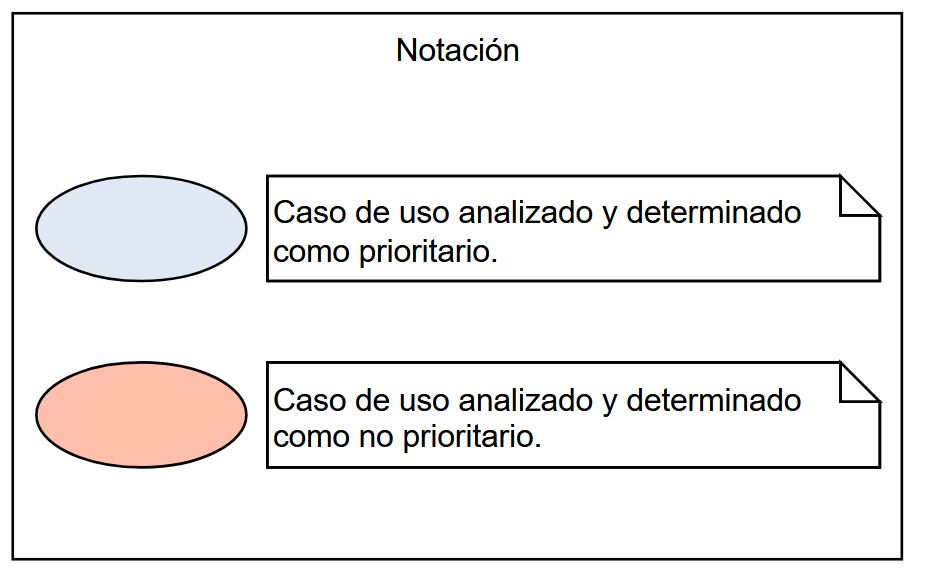
\includegraphics[width=.35\textwidth]{images/Notacion}}
		\caption{Análisis de viabilidad de los casos de uso.}
		\label{fig:Notacion}
	\end{center}
\end{figure}

Ahora comenzaremos con la explicación de la notación usada para el diagrama de casos de uso. En la figura \ref{fig:Notacion} se puede ver la notación usada para el diagrama de casos de uso, en este se puede observar que se usaron 2 colores para clasificarlos; los casos de uso de color azul fueron analizados y determinados como prioritarios y los casos de uso de color rojo fueron analizados y determinados como no prioritarios.

Decidimos determinar como casos de uso prioritarios a todos los casos del sistema móvil porque son los casos que son propios de nuestro sistema y son la parte principal de nuestro trabajo terminal y la más representativa ya que posee el mayor enfoque de inteligencia artificial, por otro lado, decidimos tomar los casos de uso del personal de la DAE como necesarios porque con ellos se justificaría la obtención de la credencial mediante el uso del proceso de la credencialización, también decidimos usar la parte de consultas y altas de los CRUD de: periodo de ETS, ETS, alumnos, docentes y personal de seguridad. Esto para representar los procesos que se realizan en el SAES y la DAE para mejorar el entendimiento, sin embargo, usar el resto del CRUD y los demás procesos de la DAE y el SAES quedan fuera del alcance del proyecto ya que se separan de la idea principal del trabajo terminal, además de que consumirán bastante tiempo y no están enfocados a la inteligencia artificial.

\section{Estructura de usuarios }

\begin{figure}[htbp!]
	\begin{center}
		\fbox{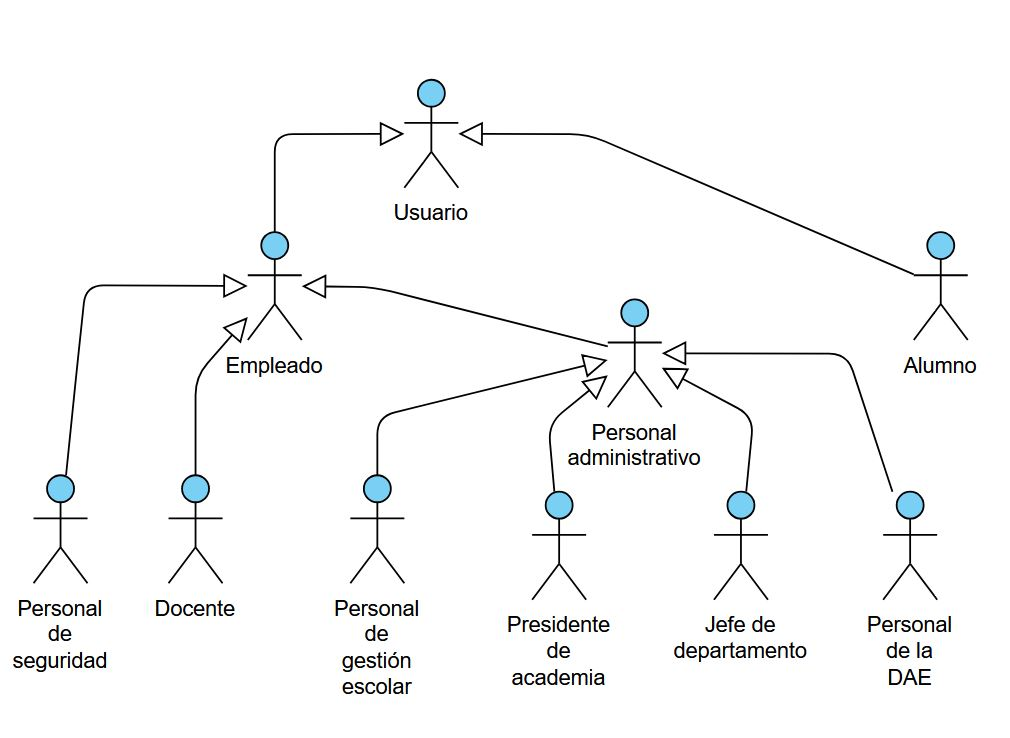
\includegraphics[width=.8\textwidth]{images/EstructuraU}}
		\caption{Estructura de los usuarios.}
		\label{fig:EstructuraU}
	\end{center}
\end{figure} 

En la figura \ref{fig:EstructuraU} se muestra la estructura de los usuarios y los tipos de usuario que están presentes en el sistema, en este se puede observar como todos los usuarios se derivan de un usuario general llamado usuario, posteriormente se divide en tipos; empleado y alumno. Después el empleado se subdivide dejando al personal de seguridad y al docente como empleados generales y creando un sub-usuario llamado personal administrativo el cual contiene al personal de gestión escolar, al presidente de academia, jefe de academia y al personal de la DAE. 

A continuación, se describirán las responsabilidades y los procesos de cada uno de los usuarios específicos (es decir los: los alumnos, personal de seguridad, docente, personal de gestión escolar, presidente de academia, jefe de departamento y personal de la DAE).

%\newpage



%\newpage

%\newpage



%---------------------------------------------------------
\section{Descripción de actores}

%---------------------------------------------------------
\begin{Usuario}{\hypertarget{tAlumno}{\subsection{Alumno}}}{
		Se refiere a las personas inscritas dentro de algún plan de estudios ofertado en la unidad académica.
	}
	\item[Responsabilidades:] \cdtEmpty
	\begin{itemize}
		\item Asistir puntualmente a las clases, prácticas y evaluaciones.
		\item Respetar a docentes, compañeros y personal administrativo.
		\item Cumplir con los requisitos y actividades de las asignaturas inscritas, incluyendo tareas, proyectos y exámenes.
		\item Realizar oportunamente los trámites escolares como inscripciones, reinscripciones, solicitudes de documentos oficiales, etc.
		\item Portar credencial institucional en todo momento.
	\end{itemize}
	

\end{Usuario}

\begin{Usuario}{\hypertarget{tPersonalSeguridad}{\subsection{Personal de seguridad}}}{
		Se refiere a las personas registradas como empleados y que permiten o no el acceso a la unidad académica.
	}
	\item[Responsabilidades:] \cdtEmpty
	\begin{itemize}
		\item Supervisar el acceso y la salida de alumnos, personal docente y visitantes, asegurándose de que cumplan con los protocolos establecidos.
		\item Verificar la identificación de las personas que ingresan a las instalaciones.
		\item Responder de manera oportuna a incidentes o emergencias dentro de las instalaciones.
		\item Brindar apoyo al personal, docentes o alumnos en caso de accidentes o situaciones de riesgo.
	\end{itemize}
	

\end{Usuario}

\begin{Usuario}{\hypertarget{tDocenteAplicador}{\subsection{Docente}}}{
		Se refiere a las personas registradas como empleados que dan clases a los alumnos y supervisan los ETS asignados.
	}
	\item[Responsabilidades:] \cdtEmpty
	\begin{itemize}
		\item Impartir las clases de manera clara, puntual y completa, cumpliendo con los objetivos de aprendizaje.
		\item Diseñar y aplicar instrumentos de evaluación justos, objetivos y alineados con los contenidos del curso.
		\item Orientar a los alumnos en el desarrollo de competencias y habilidades.
		\item Resolver dudas o problemáticas académicas dentro y fuera del aula, cuando sea necesario.
		\item Registrar la asistencia de los alumnos y reportar incidencias graves.
		\item Cumplir con la entrega de calificaciones y reportes en tiempo y forma.

	\end{itemize}
	

\end{Usuario}

\begin{Usuario}{\hypertarget{tPersonalGestion}{\subsection{Personal de gestión escolar}}}{
		Se refiere a las personas registradas como empleados y personal administrativo que realiza los procesos administrativos dentro de la ESCOM.
	}
	\item[Responsabilidades:] \cdtEmpty
	\begin{itemize}

		\item Gestionar el proceso de inscripción y reinscripción de los alumnos, verificando que cumplan con los requisitos establecidos.
		\item Mantener y actualizar el historial académico de los alumnos en los sistemas institucionales.
		\item Revisar y validar actas de nacimiento, certificados y otros documentos oficiales requeridos para el registro de los alumnos.
		\item Atender solicitudes y problemáticas relacionadas con registros, certificados, bajas temporales y procesos extraordinarios.
		\item Brindar orientación a alumnos y docentes sobre trámites escolares, fechas importantes y normatividad académica.
	\end{itemize}


\end{Usuario}

\begin{Usuario}{\hypertarget{tPersonalDAE}{\subsection{Personal de la DAE}}}{
		Se refiere a las personas registradas como empleados y personal administrativo que realiza los procesos administrativos dentro de la DAE.
	}
	\item[Responsabilidades:] \cdtEmpty
	\begin{itemize}

		\item Fomentar y coordinar actividades extracurriculares que complementen la formación académica, como talleres, conferencias, eventos culturales y deportivos.
		\item Supervisar programas de apoyo académico, como tutorías, orientación educativa y psicológica.
		\item Difundir información sobre programas de movilidad académica, intercambios, convenios nacionales e internacionales y programas de servicio social.
		\item Gestionar y emitir las credenciales oficiales del IPN para los alumnos.
		\item Verificar que los documentos requeridos para la emisión de la credencial estén completos y sean válidos.
		\item Coordinar el proceso de inscripción de los alumnos.
		\item Actualizar y mantener los registros académicos y administrativos de los alumnos. 
	\end{itemize}


\end{Usuario}

\begin{Usuario}{\hypertarget{tPresidente}{\subsection{Presidente de academia}}}{
	Se refiere a las personas registradas como empleados y personal administrativo que lidera la academia de una unidad académica o área de conocimiento dentro de la ESCOM.
	}
	\item[Responsabilidades:] \cdtEmpty
	\begin{itemize}

		\item Convocar y presidir las reuniones de academia, donde se toman decisiones sobre planes y programas de estudio.
		\item Coordinar la creación o actualización de planes y programas de estudio conforme a las necesidades del mercado laboral y las directrices institucionales.
		\item Verificar que los contenidos impartidos por los docentes sean consistentes con los objetivos de los programas.
		\item Detectar necesidades de capacitación entre los docentes y promover cursos o talleres. 
	\end{itemize}

\end{Usuario}

\begin{Usuario}{\hypertarget{tJefe}{\subsection{Jefe de departamento}}}{
	Se refiere a las personas registradas como empleados y personal administrativo que supervisa las actividades de una o más unidades académicas dentro de ESCOM.
}
\item[Responsabilidades:] \cdtEmpty
\begin{itemize}

	\item Administrar los recursos humanos y materiales asignados al departamento.
	\item Supervisar la implementación de los programas de estudio y el cumplimiento de los objetivos educativos.
	\item Promover y coordinar proyectos de investigación, desarrollo tecnológico o vinculación relacionados con el departamento.
	\item Atender quejas, sugerencias o problemas que surjan en el departamento, ya sea entre docentes o alumnos.
\end{itemize}

\end{Usuario}

\section{Diagramas de casos de uso}

A continuación se muestran los diagramas de casos de uso:

\begin{figure}[htbp!]
	\begin{center}
		\fbox{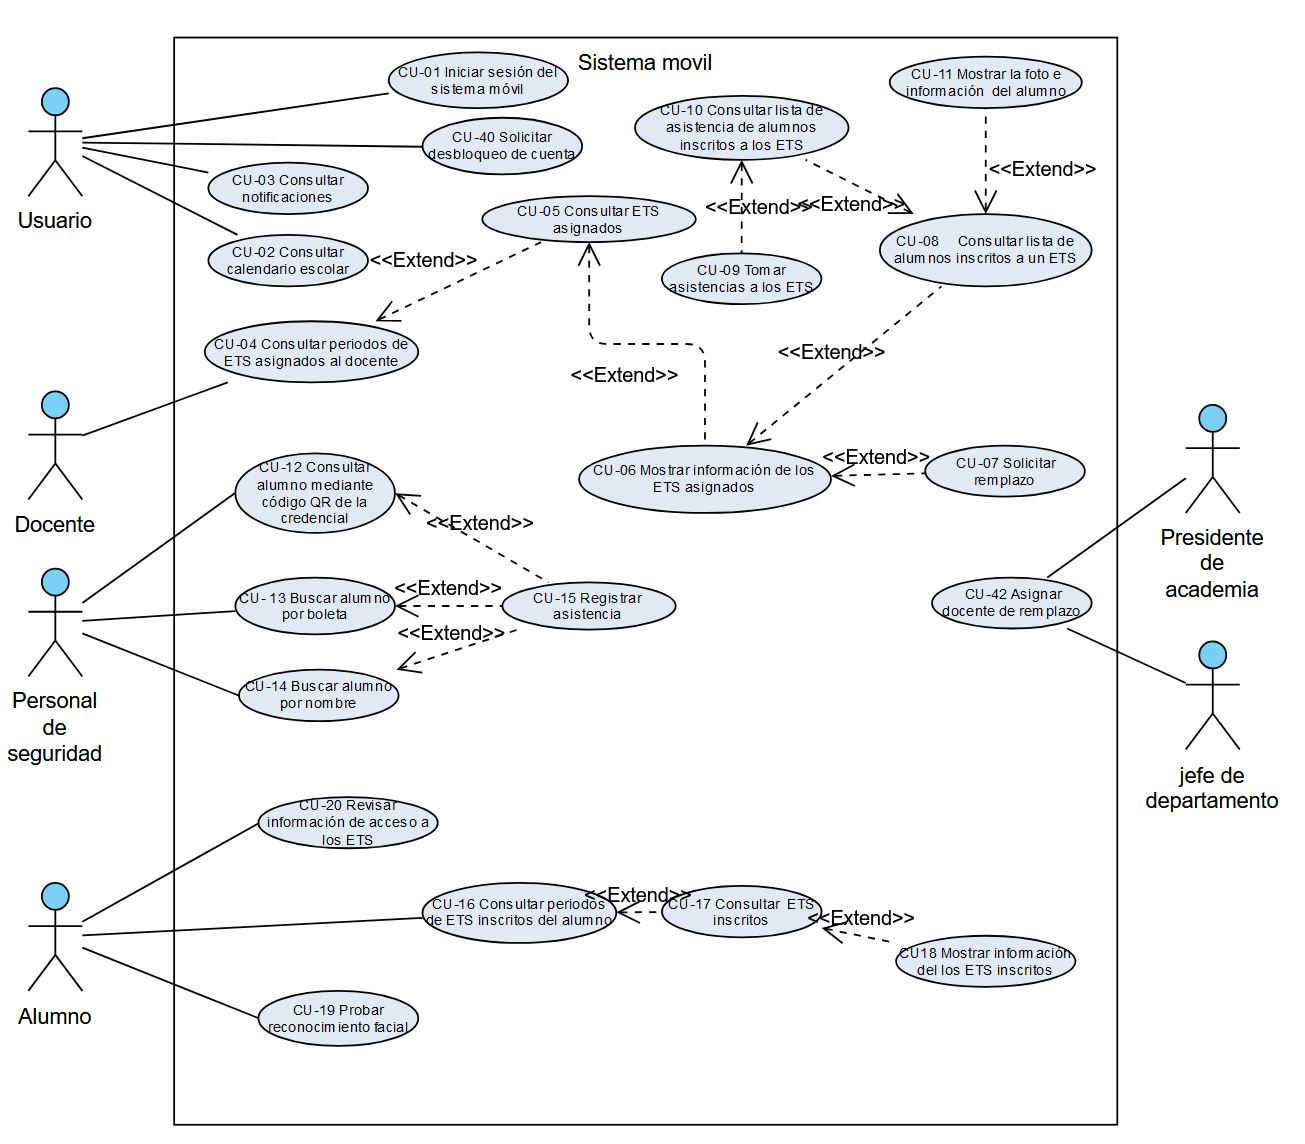
\includegraphics[width=.6\textwidth]{images/casosDeUso1}}
		\caption{Diagrama de casos de uso del sistema movil.}
		\label{fig:casosDeUso1}
	\end{center}
\end{figure}
En la figura \ref{fig:casosDeUso1} se muestra el diagrama de casos de uso del sistema móvil el cual es el sistema principal del trabajo terminal. En este diagrama se detalla la estructura del sistema, los casos de uso del docente, del alumno, del personal de seguridad, del presidente de academia y el jefe de departamento.
%\newpage
\begin{figure}[htbp!]
	\begin{center}
		\fbox{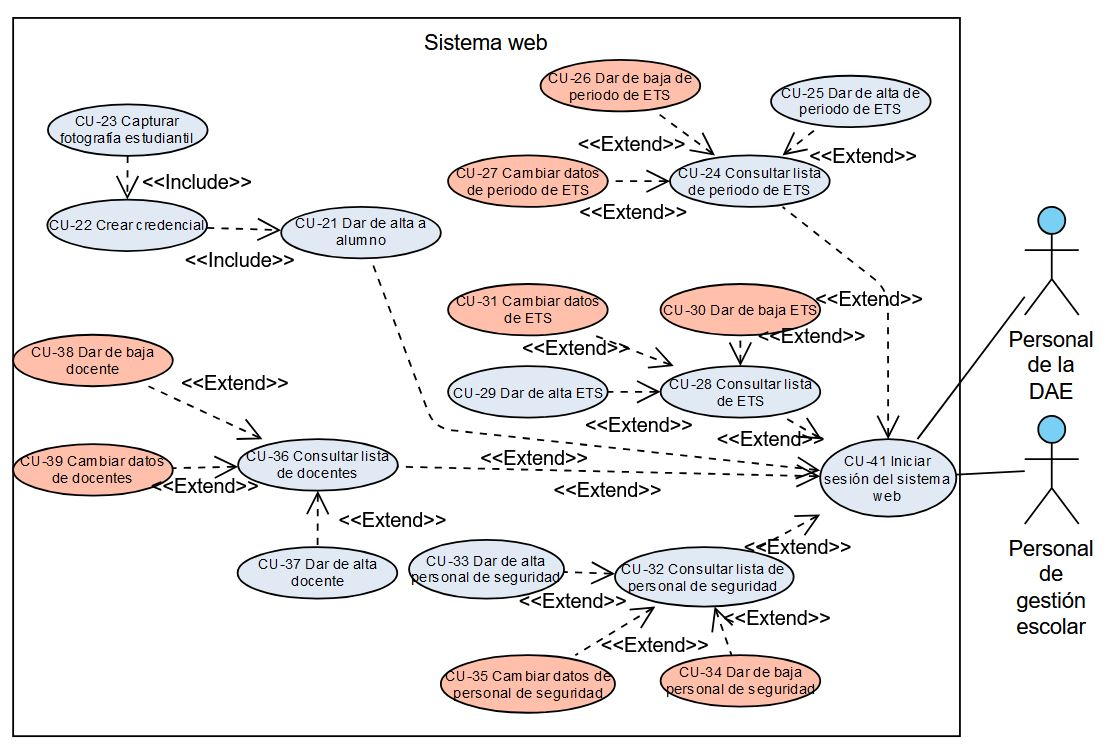
\includegraphics[width=.6\textwidth]{images/casosDeUso2}}
		\caption{Diagrama de casos de uso del sistema web.}
		\label{fig:casosDeUso2}
	\end{center}
\end{figure}

En la figura \ref{fig:casosDeUso2} se muestra el diagrama de casos de uso del sistema web el cual es el sistema secundario (la simulación de una parte del SAES y de la DAE) del trabajo terminal. En este diagrama se detalla la estructura del sistema, los casos de uso personal de la DAE y el personal de gestión escolar.

A continuación se detallan los casos de uso.

\section{Especificación de casos de uso }

%---------------------------------------------------------
% CASOS DE USO

% !TeX root = ../ejemplo.tex

%--------------------------------------
\begin{UseCase}{CU01}{Iniciar sesión de personal escolar móvil}{
		Permitir que solo el personal escolar pueda acceder al sistema, además de separar completamente las funciones del alumno y el personal escolar.
	}
	\UCitem{Versión}{\color{Gray}1}
	\UCitem{Autor}{\color{Gray}Huertas Ramírez Daniel Martín}
	\UCitem{Supervisa}{\color{Gray}Ulises Vélez Saldaña.}
	\UCitem{Actor}{\hyperlink{Empleado}{Empleado} (\hyperlink{Docente}{Docente} y \hyperlink{Personal de seguridad}{Personal de seguridad})}
	\UCitem{Propósito}{Que el empelado pueda acceder al sistema móvil y sus funciones específicas. }
	\UCitem{Entradas}{\hyperlink{Empleado.RFC}{RFC}, \hyperlink{Empleado.Contraseña}{Contraseña}}
	\UCitem{Origen}{Teclado}
	\UCitem{Salidas}{Saludo del sistema, mención de su nombre.}
	\UCitem{Destino}{Pantalla \IUref{IUE01}{Pantalla Menú de docente} si es un docente o a la \IUref{IUE02}{Pantalla Menú del personal de seguridad} si es un personal de seguridad.}
	\UCitem{Precondiciones}{El empleado debe estar registrado en el sistema de la ESCOM.}
	\UCitem{Postcondiciones}{El empleado accede al sistema y podrá realizar las acciones pertinentes a su cargo.}
	\UCitem{Errores}{
		E1: Cuando falte algún dato requerido entonces el sistema muestra el mensaje {\bf MSG1-}{``Los campos no están correctamente llenados.''}
		
		E2: Cuando la cuenta esta bloqueada el sistema no deja entrar al empleado muestra el mensaje {\bf MSG2-}``Su cuenta esta bloqueada.''
		
		E3: Cuando la contraseña no corresponde al RFC ingresado el sistema no permite el acceso al empleado y se muestra el mensaje {\bf MSG3-} ``El RFC o la contraseña no corresponden con ningún empleado.''
		
		E4: Cuando se pierde la conexión durante el proceso, los procesos se cancelan y se muestra el mensaje {\bf MSG4-}  ``El proceso no se pudo realizar por un falló de red.''
		
		E5: Cuando se intenta iniciar varias veces sesión sin éxito la cuenta es bloqueada por seguridad y se muestra el mensaje {\bf MSG5-}  ``Su cuenta ha sido bloqueada por la gran cantidad de intentos de inicio sesión fallidos''.
	}
	\UCitem{Tipo}{Caso de uso primario}
	\UCitem{Observaciones}{}
\end{UseCase}
%--------------------------------------

\begin{UCtrayectoria}
	\UCpaso[\UCactor] Introduce su RFC y contraseña en el sistema vía la \IUref{IU01}{Pantalla de Iniciar sesión de personal escolar móvil}\label{CU01.introduceDatos}.
	\UCpaso[\UCactor] Confirma la operación presionando el botón \IUbutton{Entrar}.
	\UCpaso Verifica que todos los datos requeridos hayan sido capturados.
	\UCpaso Verifica que el empleado este registrado en el sistema.
	\UCpaso Verifica que la cuenta del empleado no este bloqueada.
	\UCpaso Verifica que la contraseña corresponda al RFC.
	\UCpaso Verifica que tipo acceso tiene este empleado.
	\UCpaso La sesión es iniciada con éxito.
	\UCpaso El Empleado es redirigido a la pantalla \IUref{IUE01}{Pantalla Menú de docente} si es un docente o a la pantalla \IUref{IUE02}{Menú de personal de seguridad} si es un personal de seguridad.
	
\end{UCtrayectoria}







\newpage

% !TeX root = ../ejemplo.tex

%--------------------------------------
\begin{UseCase}{CU-02}{Consultar calendario escolar}{
    Permitir que los usuarios vean el calendario escolar y puedan solicitar al sistema que les mencioné cuantos días faltan para que inicie el próximo periodo de ETS.
}
    \UCitem{Versión}{\color{Gray}1}
    \UCitem{Autor}{\color{Gray}Huertas Ramírez Daniel Martín}
    \UCitem{Supervisa}{\color{Gray}De la Cruz de la Cruz Alejandra.}
    \UCitem{Actor}{\hyperlink{Usuario}{Usuario}}
    \UCitem{Propósito}{Que el usuario consulte cuantos días faltan para el próximo periodo de ETS.}
    \UCitem{Entradas}{Ninguna}
    \UCitem{Origen}{Pantalla táctil}
    \UCitem{Salidas}{Menciona cuantos días faltan para el periodo de ETS o si menciona que ya es periodo de ETS.}
    \UCitem{Destino}{Ninguno}
    \UCitem{Precondiciones}{El usuario debe de haber iniciado sesión.}
    \UCitem{Postcondiciones}{El usuario recibe información sobre la fecha del periodo de ETS actual.}
    \UCitem{Errores}{
        E1: Cuando es periodo de ETS el sistema muestra el mensaje {\bf MSG-6}{``Actualmente es periodo de ETS.''}

        E2: Cuando no se ha establecido un periodo de ETS actual, el sistema muestra el mensaje {\bf MSG-7}{``Actualmente el periodo de ETS no ha sido establecido.''}
    
    }
    \UCitem{Tipo}{Caso de uso primario}
    \UCitem{Observaciones}{Ninguna}
\end{UseCase}
%-------------------------------------- 

\begin{UCtrayectoria}
    \UCpaso[\UCactor] El usuario accede a la pantalla \IUref{IU02}{Pantalla Consultar calendario escolar}\label{CU02.introduceDatos} para la app móvil y \IUref{IU02-2}{Pantalla Consultar calendario escolar} para el sistema web mediante el botón con forma de calendario en cualquier pantalla excepto el inicio de sesión.
    \UCpaso[\UCactor] El usuario decide consultar cuantos días faltan para que el periodo de ETS inicie oprimiendo el botón\IUbutton{Calcular cuantos días faltan para el periodo de ETS}.
    \UCpaso El sistema calcula cuantos días faltan tomando el día actual y el día de inicio del periodo de ETS.
    \UCpaso El sistema regresa cuantos días faltan para que el periodo de ETS inicie.
    \UCpaso [\UCactor] El usuario verifica cuantos días faltan para que inicie el periodo de ETS.
\end{UCtrayectoria}








\newpage

% !TeX root = ../ejemplo.tex

%--------------------------------------
\begin{UseCase}{CU-03}{Consultar notificaciones}{
    Permitir a los usuarios revisar sus notificaciones con más detenimiento y establecerlas como leídas.
}
    \UCitem{Versión}{\color{Gray}1}
    \UCitem{Autor}{\color{Gray}Huertas Ramírez Daniel Martín}
    \UCitem{Supervisa}{\color{Gray}De la Cruz de la Cruz Alejandra.}
    \UCitem{Actor}{\hyperlink{Usuario}{Usuario}}
    \UCitem{Propósito}{Que el usuario revise sus notificaciones con detenimiento y las establezca como leídas.}
    \UCitem{Entradas}{Ninguna}
    \UCitem{Origen}{Pantalla táctil}
    \UCitem{Salidas}{Menciona que la notificación seleccionada ha sido establecida como leída.}
    \UCitem{Destino}{Ninguno}
    \UCitem{Precondiciones}{El usuario debe de haber iniciado sesión.}
    \UCitem{Postcondiciones}{El usuario revisó sus notificaciones.}
    \UCitem{Errores}{
        E1: Cuando el usuario no tiene notificaciones el sistema muestra el mensaje {\bf MSG-8}{``Actualmente no hay notificaciones.''}    
    }
    \UCitem{Tipo}{Caso de uso primario}
    \UCitem{Observaciones}{}

\end{UseCase}
%-------------------------------------- 

\begin{UCtrayectoria}
    \UCpaso[\UCactor] El usuario accede a la pantalla \IUref{IU03}{Pantalla Consultar notificaciones}\label{CU03.introduceDatos} para la app móvil  mediante el botón con forma de campana en cualquier pantalla excepto los inicios de sesión.
    \UCpaso[\UCactor] El usuario decide consultar sus notificaciones más actuales \Trayref{A}.
    \UCpaso[\UCactor] El usuario marco como leídas las notificaciones que acaba de leer mediante el botón con forma de palomita especifico de cada notificación.
    \UCpaso El sistema marca como leídas las notificaciones.

\end{UCtrayectoria}

\begin{UCtrayectoriaA}{A}{El usuario quiere consultar las notificaciones de una fecha específica}
	\UCpaso[\UCactor] El usuario usa el buscador de la parte superior para buscar notificaciones según su fecha.
	\UCpaso[\UCactor] El usuario marco como leídas las notificaciones que acaba de leer mediante el botón con forma de palomita especifico de cada notificación.
	\UCpaso El sistema marca como leídas las notificaciones.

\end{UCtrayectoriaA}



\newpage

% \IUref{IUAdmPS}{Administrar Planta de Selección}
% \IUref{IUModPS}{Modificar Planta de Selección}
% \IUref{IUEliPS}{Eliminar Planta de Selección}

%-------------------------------------- COMIENZA descripción del caso de uso.

%\begin{UseCase}[archivo de imágen]{UCX}{Nombre del Caso de uso}{
%--------------------------------------
\begin{UseCase}{CU-04}{Consultar periodos de ETS asignados al docente}{
		Este caso de uso permite al docente consultar los periodos de ETS que tiene asignados. 
	}
	\UCitem{Versión}{\color{Gray}1.0}
	\UCitem{Autor}{\color{Gray}De la cruz De la cruz Alejandra}
	\UCitem{Supervisa}{\color{Gray}Ulises Velez Saldaña}
	\UCitem{Actor}{\hyperlink{Docente}{Docente}}
	\UCitem{Propósito}{Permitir al docente consultar los periodos de ETS que le han sido asignados.}
	\UCitem{Entradas}{Ninguna}
	\UCitem{Origen}{Pantalla táctil}
	\UCitem{Salidas}{Lista de periodos de ETS asignados.}
	\UCitem{Destino}{\IUref{IU04}{Pantalla Periodo de ETS}}
	\UCitem{Precondiciones}{El docente debe estar autenticado en el sistema.}
	\UCitem{Postcondiciones}{El docente ha consultado los periodos de ETS asignados.}
	\UCitem{Errores}{
			E1:El sistema no puede recuperar la información de los periodos.
			
			E2: No hay periodos de ETS asignados al docente. }
	\UCitem{Tipo}{Se extiende del CU}
	\UCitem{Observaciones}{Ninguna}
\end{UseCase}
%--------------------------------------
\begin{UCtrayectoria}
	\UCpaso[\UCactor] Accede a la \IUref{IUE01}{Pantalla Menú del docente} después de haber iniciado sesión.
	\UCpaso[\UCactor] Presiona el botón \IUbutton{Consultar periodos de ETS}.
	\UCpaso Verifica que el docente cuente con periodos de ETS. \Trayref{A}.
	\UCpaso Busca en la base de datos los periodos de ETS asignados al docente.
	\UCpaso Despliega la lista de periodos de ETS asignados al docente en la \IUref{IU04}{Pantalla Periodo de ETS}.
\end{UCtrayectoria}
%--------------------------------------        
\begin{UCtrayectoriaA}{A}{No hay periodos asignados al docente}
	\UCpaso Verifica y no encuentra registros de periodos de ETS asignados al docente.
	\UCpaso Muestra un mensaje: {\bf MSG10-}{``No hay periodos de ETS asignados.''}
	\UCpaso[\UCactor] Presiona el botón \IUbutton{Regresar} para volver a la pantalla anterior.
	\UCpaso Fin de la trayectoria alternativa.
\end{UCtrayectoriaA}
%--------------------------------------        
\begin{UCtrayectoriaA}{B}{Error en la conexión con la base de datos}
	\UCpaso Muestra un mensaje de error: {\bf MSG11-}{``Error al consultar la base de datos. Intente nuevamente más tarde.''}
	\UCpaso[\UCactor] Presiona el botón \IUbutton{Aceptar} para cerrar el mensaje.
	\UCpaso[\UCactor] Puede intentar la consulta nuevamente o presionar el botón \IUbutton{Regresar} para volver a la pantalla anterior.
	\UCpaso Fin de la trayectoria alternativa.
\end{UCtrayectoriaA}
%-------------------------------------- TERMINA descripción del caso de uso.

\newpage

% \IUref{IUAdmPS}{Administrar Planta de Selección}
% \IUref{IUModPS}{Modificar Planta de Selección}
% \IUref{IUEliPS}{Eliminar Planta de Selección}

%-------------------------------------- COMIENZA descripción del caso de uso.

%\begin{UseCase}[archivo de imágen]{UCX}{Nombre del Caso de uso}{
%--------------------------------------
\begin{UseCase}{CU-05}{Consultar ETS asignados}{
		Este caso de uso permite al docente consultar los ETS que tiene asignados.
	}
	\UCitem{Versión}{\color{Gray}1.0}
	\UCitem{Autor}{\color{Gray}De la cruz De la cruz Alejandra}
	\UCitem{Supervisa}{\color{Gray}Ulises Velez Saldaña}
	\UCitem{Actor}{\hyperlink{Docente}{Docente}}
	\UCitem{Propósito}{Permitir al docente consultar los ETS que le han sido asignados.}
	\UCitem{Entradas}{Selecciona un periodo}
	\UCitem{Origen}{Pantalla táctil}
	\UCitem{Salidas}{Lista de ETS asignados.}
	\UCitem{Destino}{\IUref{IU05}{Pantalla de Consultar ETS}}
	\UCitem{Precondiciones}{El docente debe estar autenticado en el sistema.}
	\UCitem{Postcondiciones}{El docente ha consultado los ETS asignados.}
	\UCitem{Errores}{
			E1: El sistema no puede recuperar la información de los ETS asignados.
			
			E2: No hay ETS asignados al docente.}
	\UCitem{Tipo}{Se extiende del CU01 Iniciar Sesión del docente}
	\UCitem{Observaciones}{Ninguna}
\end{UseCase}
%--------------------------------------
\begin{UCtrayectoria}
	\UCpaso[\UCactor] Selecciona el período académico que desea consultar desde la \IUref{IU04}{Pantalla Periodo de ETS}.
	\UCpaso Verifica que el docente tenga ETS asignados en el periodo seleccionado \Trayref{A}.
	\UCpaso Despliega la lista de ETS asignados al docente en la \IUref{IU05}{Pantalla de Consultar ETS}.
\end{UCtrayectoria}

%--------------------------------------        
\begin{UCtrayectoriaA}{A}{No hay ETS asignados en el periodo seleccionado}
	\UCpaso Muestra un mensaje: {\bf MSG-12-}{``No hay ETS asignados actualmente.''}
	\UCpaso[\UCactor] Presiona el botón \IUbutton{Regresar} para volver a la pantalla anterior.
	\UCpaso Fin de la trayectoria alternativa.
\end{UCtrayectoriaA}
%--------------------------------------        
\begin{UCtrayectoriaA}{B}{Error en la conexión con la base de datos}
	\UCpaso Muestra un mensaje de error: {\bf MSG11-}{``Error al consultar la base de datos. Intente nuevamente más tarde.''}
	\UCpaso[\UCactor] Presiona el botón \IUbutton{Aceptar} para cerrar el mensaje.
	\UCpaso[\UCactor] Puede intentar la consulta nuevamente o presionar el botón \IUbutton{Regresar} para volver a la pantalla anterior.
	\UCpaso Fin de la trayectoria alternativa.
\end{UCtrayectoriaA}

%-------------------------------------- TERMINA descripción del caso de uso.
\newpage

% \IUref{IUAdmPS}{Administrar Planta de Selección}
% \IUref{IUModPS}{Modificar Planta de Selección}
% \IUref{IUEliPS}{Eliminar Planta de Selección}

%-------------------------------------- COMIENZA descripción del caso de uso.

%\begin{UseCase}[archivo de imágen]{UCX}{Nombre del Caso de uso}{
%--------------------------------------
% !TeX root = ../ejemplo.tex
\begin{UseCase}{CU-06}{Mostrar información de los ETS asignados}{
	Este caso de uso permite al docente visualizar la información detallada de los ETS que tiene asignados.
}
\UCitem{Versión}{\color{Gray}1.0}
\UCitem{Autor}{\color{Gray}De la cruz De la cruz Alejandra}
\UCitem{Supervisa}{\color{Gray}Huertas Ramírez Daniel Martín}
\UCitem{Actor}{\hyperlink{PersonalAcademico}{Docente}}
\UCitem{Propósito}{Permite al docente visualizar la información detallada de cada ETS que tiene asignado.}
\UCitem{Entradas}{Ninguna}
\UCitem{Origen}{Pantalla táctil}
\UCitem{Salidas}{Detalle de ETS asignado.}
\UCitem{Destino}{\IUref{IU06}{Pantalla Información de ETS}}
\UCitem{Precondiciones}{El docente debe estar autenticado y tener ETS asignados en el sistema.}
\UCitem{Postcondiciones}{El docente ha visualizado la información detallada de sus ETS asignados.}
\UCitem{Errores}{
		E1: El sistema no puede recuperar la información detallada de los ETS y muestra el mensaje {\bf MSG-12}{``Información no disponible para el ETS seleccionado''}.
		E2: Error en la conexión con la base de datos y muestra el mensaje y muestra el mensaje {\bf MSG-9}{``Error al consultar la base de datos. Intente nuevamente más tarde.''}.
}
\UCitem{Tipo}{Se entiende del CU-05 Mostrar información de los ETS asignados}
\UCitem{Observaciones}{Ninguna}
\end{UseCase}
%--------------------------------------
\begin{UCtrayectoria}
\UCpaso[\UCactor] El docente selecciona el ETS que desea visualizar desde la \IUref{IU05}{Pantalla  Consultar ETS}.
\UCpaso[\UCsist] El sistema verifica si existen detalles disponibles para el ETS seleccionado. \Trayref{A}
\UCpaso El sistema despliega la información detallada de cada ETS asignado en la \IUref{IU06}{Pantalla Información de ETS}
\end{UCtrayectoria}
%--------------------------------------        
\begin{UCtrayectoriaA}{A}{No hay detalles disponibles para el ETS seleccionado}
\UCpaso El sistema muestra un mensaje: {\bf MSG-12}{``Información no disponible para el ETS seleccinado''}
\UCpaso[\UCactor] El docente presiona el botón \IUbutton{Regresar} para volver a la lista de ETS.
\UCpaso Fin de la trayectoria alternativa.
\end{UCtrayectoriaA}

%--------------------------------------        
\begin{UCtrayectoriaA}{B}{Error en la conexión con la base de datos}
\UCpaso El sistema muestra un mensaje de error: {\bf MSG-9}{``Error al consultar la base de datos. Intente nuevamente más tarde.''}
\UCpaso[\UCactor] El docente presiona el botón \IUbutton{Aceptar} para cerrar el mensaje.
\UCpaso[\UCactor] El docente puede intentar la consulta nuevamente o presionar el botón \IUbutton{Regresar} para volver a la pantalla anterior.
\UCpaso Fin de la trayectoria alternativa.
\end{UCtrayectoriaA}

%-------------------------------------- TERMINA descripción del caso de uso.


\newpage

% \IUref{IUAdmPS}{Administrar Planta de Selección}
% \IUref{IUModPS}{Modificar Planta de Selección}
% \IUref{IUEliPS}{Eliminar Planta de Selección}

%-------------------------------------- COMIENZA descripción del caso de uso.

%\begin{UseCase}[archivo de imágen]{UCX}{Nombre del Caso de uso}{
%--------------------------------------
\begin{UseCase}{CU-07}{Asignar docente ayudante}{
		Este caso de uso permite a un docente solicitar la asignación de un docente ayudante para aplicar el ETS en su lugar en caso de no poder asistir.
	}
	\UCitem{Versión}{\color{Gray}1.0}
	\UCitem{Autor}{\color{Gray}De la cruz De la cruz Alejandra}
	\UCitem{Supervisa}{\color{Gray}Ulises Velez Saldaña}
	\UCitem{Actor}{\hyperlink{Docente}{Docente}}
	\UCitem{Propósito}{Permitir al docente asignado para un ETS solicitar ayuda de otro docente para realizar la aplicación en su lugar.}
	\UCitem{Entradas}{
		\begin{itemize}
			\item Identificador del ETS.
			\item Identificador del docente ayudante solicitado.
		\end{itemize}
	}
	\UCitem{Origen}{Teclado}
	\UCitem{Salidas}{Confirmación de la asignación del docente ayudante.}
	\UCitem{Destino}{{\bf MSG-14-}{``El docente ayudante ha sido asignado exitosamente para la aplicación del ETS.''}}
	\UCitem{Precondiciones}{El docente debe estar autenticado en el sistema y tener un ETS asignado.}
	\UCitem{Postcondiciones}{El docente ayudante ha sido asignado al ETS en lugar del docente asignado.}
	\UCitem{Errores}{
			E1: El sistema pierde la conexión al intentar registrar la asignación.
	}
	\UCitem{Tipo}{Se extiende del CU}
	\UCitem{Observaciones}{Ninguna}
\end{UseCase}
%--------------------------------------
\begin{UCtrayectoria}
	\UCpaso[\UCactor] El docente accede a la \IUref{IU06}{Pantalla Información de ETS}.
	\UCpaso[\UCactor] Selecciona la opción \IUbutton{Solicitar docente ayudante} para el ETS asignado.
	\UCpaso Ingresa el identificador del docente ayudante.
	\UCpaso El sistema verifica la existencia del ETS. \Trayref{A}
	\UCpaso El sistema verifica la disponibilidad del docente ayudante para la fecha del ETS. \Trayref{B} \Trayref{D}
	\UCpaso El sistema registra la asignación del docente ayudante en la base de datos. \Trayref{C}
	\UCpaso Muestra un mensaje de confirmación: {\bf MSG-14-}{``El docente ayudante ha sido asignado exitosamente para la aplicación del ETS.''}
\end{UCtrayectoria}
%--------------------------------------        
\begin{UCtrayectoriaA}{A}{El ETS no existe o ya ha sido aplicado}
	\UCpaso[\UCactor] El sistema muestra un mensaje: {\bf MSG-15-}{``El ETS especificado no existe o ya ha sido aplicado. Verifique la información e intente nuevamente.''}
	\UCpaso[\UCactor] El docente puede reingresar el identificador del ETS o regresar a la pantalla anterior.
	\UCpaso Fin de la trayectoria alternativa.
\end{UCtrayectoriaA}
%--------------------------------------        
\begin{UCtrayectoriaA}{B}{Docente ayudante no disponible en la fecha}
	\UCpaso El sistema detecta que el docente ayudante solicitado no está disponible para la fecha del ETS.
	\UCpaso[\UCactor] El sistema muestra un mensaje: {\bf MSG-16-}{``El docente ayudante no está disponible en la fecha especificada.''}
	\UCpaso[\UCactor] El docente puede seleccionar otro docente o intentar una nueva asignación.
	\UCpaso Fin de la trayectoria alternativa.
\end{UCtrayectoriaA}
%--------------------------------------        
\begin{UCtrayectoriaA}{C}{Error al registrar la asignación}
	\UCpaso Ocurrió un error al intentar registrar la asignación en la base de datos debido a una pérdida de conexión.
	\UCpaso[\UCactor] El sistema muestra un mensaje de error:  {\bf MSG-4} {``El proceso no se pudo realizar por un falló de red.''}
	\UCpaso[\UCactor] El docente presiona \IUbutton{Aceptar} y puede intentar la asignación nuevamente más tarde.
	\UCpaso Fin de la trayectoria alternativa.
\end{UCtrayectoriaA}
%--------------------------------------
\begin{UCtrayectoriaA}{D}{Docente ayudante ya asignado en otro ETS}
	\UCpaso El sistema detecta que el docente solicitado ya está asignado como ayudante en otro ETS en la misma fecha y horario.
	\UCpaso[\UCactor] El sistema muestra un mensaje: {\bf MSG-17-}{``El docente ya está asignado en otro ETS en el mismo horario.''}
	\UCpaso[\UCactor] El docente solicitante puede elegir otro docente o ajustar la fecha de solicitud.
	\UCpaso Fin de la trayectoria alternativa.
\end{UCtrayectoriaA}

%-------------------------------------- TERMINA descripción del caso de uso.
\newpage

% \IUref{IUAdmPS}{Administrar Planta de Selección}
% \IUref{IUModPS}{Modificar Planta de Selección}
% \IUref{IUEliPS}{Eliminar Planta de Selección}

%-------------------------------------- COMIENZA descripción del caso de uso.

%\begin{UseCase}[archivo de imágen]{UCX}{Nombre del Caso de uso}{
%--------------------------------------
\begin{UseCase}{CU-08}{Consultar lista de alumnos inscritos a un ETS}{
		Este caso de uso permite al docente consultar la lista de los alumnos inscritos a un ETS asignado.
	}
	\UCitem{Versión}{\color{Gray}1.0}
	\UCitem{Autor}{\color{Gray}De la cruz De la cruz Alejandra}
	\UCitem{Supervisa}{\color{Gray}Huertas Ramírez Daniel Martín}
	\UCitem{Actor}{\hyperlink{PersonalAcademico}{Docente}}
	\UCitem{Propósito}{Permitir al docente visualizar la lista de alumnos inscritos en un ETS para verificar su asistencia.}
	\UCitem{Entradas}{Ninguna}
	\UCitem{Origen}{Pantalla táctil}
	\UCitem{Salidas}{Lista de los alumnos inscritos al ETS.}
	\UCitem{Destino}{\IUref{IU13}{Pantalla consultar lista de alumnos inscritos a un ETS}.}
	\UCitem{Precondiciones}{El docente debe estar autenticado y tener asignado el ETS correspondiente.}
	\UCitem{Postcondiciones}{El docente ha visualizado la lista de asistencia de los alumnos inscritos al ETS.}
	\UCitem{Errores}{
			E1: El ETS seleccionado no tiene alumnos inscritos y se muestra el mensaje {\bf MSG-14}{``No hay alumnos inscritos en este ETS.''}.
			
			E2: El sistema pierde la conexión al intentar recuperar la lista de asistencia y se muestra el mensaje {\bf MSG-9}{``Error al consultar la base de datos. Intente nuevamente más tarde.''}.
	}
	\UCitem{Tipo}{Se entiende del CU06 Mostrar información de los ETS asignados}
	\UCitem{Observaciones}{Ninguna}
\end{UseCase}
%--------------------------------------
\begin{UCtrayectoria}
	\UCpaso[\UCactor] El docente presiona el botón \IUbutton{Ver alumnos} desde la pantalla \IUref{IU06}{Pantalla de Información de ETS}.
	\UCpaso El sistema verifica la existencia del ETS y que tenga alumnos inscritos. \Trayref{A}.
	\UCpaso El sistema recupera la lista de alumnos inscritos en el ETS. \Trayref{B}
	\UCpaso El sistema muestra la lista de alumnos inscritos en la \IUref{IU13}{Pantalla consultar lista de alumnos inscritos a un ETS}.
\end{UCtrayectoria}

%--------------------------------------        
\begin{UCtrayectoriaA}{A}{El ETS no tiene alumnos inscritos}
	\UCpaso El sistema muestra un mensaje: {\bf MSG-14}{``No hay alumnos inscritos en este ETS.''}
	\UCpaso[\UCactor] El docente presiona el botón \IUbutton{Regresar} para volver a la pantalla anterior donde se muestra la información detallada del ETS.
	\UCpaso Fin de la trayectoria alternativa.
\end{UCtrayectoriaA}
%--------------------------------------        
\begin{UCtrayectoriaA}{B}{Error en la conexión con la base de datos}
	\UCpaso El sistema muestra un mensaje de error: {\bf MSG-9}{``Error al consultar la base de datos. Intente nuevamente más tarde.''}
	\UCpaso[\UCactor] El docente presiona el botón \IUbutton{Aceptar} para cerrar el mensaje.
	\UCpaso[\UCactor] El docente puede intentar la consulta nuevamente.
	\UCpaso Fin de la trayectoria alternativa.
\end{UCtrayectoriaA}
%-------------------------------------- TERMINA descripción del caso de uso.

\newpage

% \IUref{IUAdmPS}{Administrar Planta de Selección}
% \IUref{IUModPS}{Modificar Planta de Selección}
% \IUref{IUEliPS}{Eliminar Planta de Selección}

%-------------------------------------- COMIENZA descripción del caso de uso.

%\begin{UseCase}[archivo de imágen]{UCX}{Nombre del Caso de uso}{
%--------------------------------------
\begin{UseCase}{CU-09}{Tomar asistencias a los ETS}{
		Este caso de uso permite al docente registrar la asistencia de los alumnos inscritos a un ETS asignado.
	}
	\UCitem{Versión}{\color{Gray}1.0}
	\UCitem{Autor}{\color{Gray}De la cruz De la cruz Alejandra}
	\UCitem{Supervisa}{\color{Gray}Huertas Ramírez Daniel Martín}
	\UCitem{Actor}{\hyperlink{Docente}{Docente}}
	\UCitem{Propósito}{Permitir al docente registrar la asistencia de los alumnos que estén inscritos a un ETS.}
	\UCitem{Entradas}{-}
	\UCitem{Origen}{Pantalla táctil}
	\UCitem{Salidas}{Confirmación del registro de asistencia de los alumnos.}
	\UCitem{Destino}{\IUref{IU08}{Lista de asistencia de ETS.}}
	\UCitem{Precondiciones}{El docente debe estar autenticado y asignado al ETS correspondiente.}
	\UCitem{Postcondiciones}{La asistencia de los alumnos ha sido registrada en el sistema para el ETS.}
	\UCitem{Errores}{
		\begin{itemize}
			\item El ETS seleccionado no tiene alumnos inscritos y se muestra el mensaje {\bf MSG-16}{``No hay alumnos inscritos en este ETS.''}
			\item El sistema pierde la conexión al intentar registrar la asistencia y se muestra el mensaje {\bf MSG-9}{``Error al consultar la base de datos. Intente nuevamente más tarde.''}
			\item El sistema no logro activar la camara y se muestra el mensaje {\bf MSG-17}{``No se pudo activar la cámara o reconocer la identidad. Intente nuevamente.''}
		\end{itemize}
	}
	\UCitem{Tipo}{Se entiende del CU-10 Consultar lista de asistencia de alumnos inscritos a los ETS}
	\UCitem{Observaciones}{}
\end{UseCase}
%--------------------------------------
\begin{UCtrayectoria}
	\UCpaso[\UCactor] El docente presiona el recuadro con la información del alumno que desee desde la pantalla \IUref{IU08}{Lista de asistencia de ETS}.
	\UCpaso El sistema le muestra una imagen del alumno al docente.
	\UCpaso[\UCactor] El docente no esta seguro de la identidad del alumno, por lo que decide usar el reconocimiento facial, accediendo a la pantalla \IUref{IU17}{Pantalla Reconocimiento facial} presionando el texto de \IUbutton{Estatus}. \Trayref{A} \Trayref{B}
	\UCpaso El sistema activa la cámara y comienza el proceso de reconocimiento facial de los alumnos presentes \IUref{IU17}{Pantalla Reconocimiento facial}. \Trayref{C} \Trayref{D}
	\UCpaso El sistema analiza la imagen de cada alumno y muestra un indicador:
	\begin{itemize}
		\item Verde: El sistema está casi seguro de que la persona es quien dice ser y muestra las características coincidentes.
		\item Amarillo: El sistema no está seguro y necesita la ayuda del docente para confirmar la identidad, mostrando tanto las características coincidentes como las que no coinciden. \Trayref{E}
		\item Rojo: El sistema está casi seguro de que la persona no es quien dice ser y muestra las características que no coinciden. \Trayref{F}
	\end{itemize}
	\UCpaso[\UCactor] El docente revisa las características del alumno y decide si confirma la identidad del alumno cuando el indicador marque el color Amarillo. 
	\UCpaso El sistema marca la asistencia de cada alumno.
	\UCpaso[\UCactor] El docente confirma el registro de asistencia.
	\UCpaso El sistema guarda la asistencia y muestra un mensaje de confirmación: {\bf MSG-15}{``Asistencia registrada exitosamente.''}
	\UCpaso El sistema muestra la lista de asistencia de los alumnos en la \IUref{IU08}{Pantalla Lista de asistencia de ETS.}
\end{UCtrayectoria}
%--------------------------------------        
\begin{UCtrayectoriaA}{A}{El Docente está seguro de la identidad del alumno sin la necesidad de usar el reconocimiento facial y decide que le registrara asistencia sin la necesidad del reconocimiento facial}
	\UCpaso[\UCactor] El docente presiona el botón \IUbutton{Registrar asistencia}.
	\UCpaso El sistema actualiza la asistencia.
	\UCpaso Fin de la trayectoria alternativa.
\end{UCtrayectoriaA}
%--------------------------------------        
\begin{UCtrayectoriaA}{B}{El Docente no está seguro de la identidad del alumno sin la necesidad de usar el reconocimiento facial y decide que no le registrara asistencia}
	\UCpaso[\UCactor] El docente presiona el botón \IUbutton{No registrar asistencia}.
	\UCpaso El sistema no actualiza la asistencia.
	\UCpaso Fin de la trayectoria alternativa.
\end{UCtrayectoriaA}        
%--------------------------------------        
\begin{UCtrayectoriaA}{C}{El ETS no tiene alumnos inscritos}
	\UCpaso El sistema muestra un mensaje: {\bf MSG-16}{``No hay alumnos inscritos en este ETS.''}
	\UCpaso[\UCactor] El docente presiona el botón \IUbutton{Regresar} para volver a la pantalla anterior.
	\UCpaso Fin de la trayectoria alternativa.
\end{UCtrayectoriaA}
%--------------------------------------        
\begin{UCtrayectoriaA}{D}{Error en la conexión con la base de datos}
	\UCpaso El sistema muestra un mensaje de error: {\bf MSG-9}{``Error al consultar la base de datos. Intente nuevamente más tarde.''}
	\UCpaso[\UCactor] El docente presiona el botón \IUbutton{Aceptar} para cerrar el mensaje.
	\UCpaso[\UCactor] El docente puede intentar registrar la asistencia.
	\UCpaso Fin de la trayectoria alternativa.
\end{UCtrayectoriaA}
%--------------------------------------        
\begin{UCtrayectoriaA}{E}{El sistema detecta incertidumbre en la identidad de un alumno}
	\UCpaso El sistema detecta las características coincidentes como las que no coinciden con el alumno.
	\UCpaso[\UCactor] El docente revisa la información proporcionada y toma una decisión sobre la identidad del alumno.
	\UCpaso[\UCactor] El docente confirma o corrige la asistencia.
	\UCpaso El sistema actualiza la asistencia según la confirmación del docente.
	\UCpaso El sistema muestra la lista de asistencia de los alumnos actualizada en la \IUref{IU08}{Pantalla Lista de asistencia de ETS}.
	\UCpaso Fin de la trayectoria alternativa.
\end{UCtrayectoriaA}
%--------------------------------------        
\begin{UCtrayectoriaA}{F}{El sistema identifica que el alumno no coincide con la foto registrada}
	\UCpaso El sistema muestra al docente las características que no coinciden.
	\UCpaso[\UCactor] El docente revisa las discrepancias y decide marcar al alumno como ausente o realizar una verificación adicional.
	\UCpaso El sistema actualiza la asistencia.
	\UCpaso El sistema muestra la lista de asistencia de los alumnos actualizada en la \IUref{IU08}{Pantalla Lista de asistencia de ETS}.
	\UCpaso Fin de la trayectoria alternativa.
\end{UCtrayectoriaA}

%-------------------------------------- TERMINA descripción del caso de uso.
\newpage

% \IUref{IUAdmPS}{Administrar Planta de Selección}
% \IUref{IUModPS}{Modificar Planta de Selección}
% \IUref{IUEliPS}{Eliminar Planta de Selección}

%-------------------------------------- COMIENZA descripción del caso de uso.

%\begin{UseCase}[archivo de imágen]{UCX}{Nombre del Caso de uso}{
%--------------------------------------
\begin{UseCase}{CU-10}{Consultar lista de asistencia de alumnos inscritos a los ETS}{
		Este caso de uso permite al docente visualizar la asistencia de los alumnos inscritos a un ETS asignado.
	}
	\UCitem{Versión}{\color{Gray}1.0}
	\UCitem{Autor}{\color{Gray}De la cruz De la cruz Alejandra}
	\UCitem{Supervisa}{\color{Gray}Huertas Ramírez Daniel Martin}
	\UCitem{Actor}{\hyperlink{Docente}{Docente}}
	\UCitem{Propósito}{Permitir al docente registrar la asistencia de los alumnos que estén inscritos a un ETS.}
	\UCitem{Entradas}{Ninguna}
	\UCitem{Origen}{Pantalla táctil}
	\UCitem{Salidas}{Confirmación del registro de asistencia de los alumnos.}
	\UCitem{Destino}{\IUref{IU08}{Lista de asistencia de ETS.}}
	\UCitem{Precondiciones}{El docente debe estar autenticado y asignado al ETS correspondiente.}
	\UCitem{Postcondiciones}{La asistencia de los alumnos ha sido registrada en el sistema para el ETS.}
	\UCitem{Errores}{
		\begin{itemize}
			\item El ETS seleccionado no tiene alumnos inscritos y se muestra el mensaje {\bf MSG-16}{``No hay alumnos inscritos en este ETS.''}
			\item El sistema pierde la conexión al intentar registrar la asistencia y se muestra el mensaje {\bf MSG-9}{``Error al consultar la base de datos. Intente nuevamente más tarde.''}
		\end{itemize}
	}
	\UCitem{Tipo}{Se entiende del CU-10 consultar lista de asistencia de alumnos inscritos a los ETS}
	\UCitem{Observaciones}{}
\end{UseCase}
%--------------------------------------
\begin{UCtrayectoria}
	\UCpaso[\UCactor] El docente presiona el botón \IUbutton{Tomar asistencia} desde la pantalla \IUref{IU13}{Pantalla Lista de alumno}.
	\UCpaso El sistema activa la cámara y comienza el proceso de reconocimiento facial de los alumnos presentes. \Trayref{A} \Trayref{B}
	\UCpaso El sistema analiza la imagen de cada alumno y muestra un indicador:
	\begin{itemize}
		\item Verde: El sistema está casi seguro de que la persona es quien dice ser y muestra las características coincidentes.
		\item Amarillo: El sistema no está seguro y necesita la ayuda del docente para confirmar la identidad, mostrando tanto las características coincidentes como las que no coinciden. \Trayref{C}
		\item Rojo: El sistema está casi seguro de que la persona no es quien dice ser y muestra las características que no coinciden. \Trayref{D}
	\end{itemize}
	\UCpaso[\UCactor] El docente revisa las características del alumno y decide si confirma la identidad del alumno cuando el indicador marque el color Amarillo. 
	\UCpaso El sistema marca la asistencia de cada alumno.
	\UCpaso[\UCactor] El docente confirma el registro de asistencia.
	\UCpaso El sistema guarda la asistencia y muestra un mensaje de confirmación: {\bf MSG-18}{``Asistencia registrada exitosamente.''}
	\UCpaso El sistema muestra la lista de asistencia de los alumnos en la \IUref{IU08}{Pantalla Lista de asistencia de ETS.}
\end{UCtrayectoria}
%--------------------------------------        
\begin{UCtrayectoriaA}{A}{El ETS no tiene alumnos inscritos}
	\UCpaso El sistema muestra un mensaje: {\bf MSG-17}{``No hay alumnos inscritos en este ETS.''}
	\UCpaso[\UCactor] El docente presiona el botón \IUbutton{Regresar} para volver a la pantalla anterior.
	\UCpaso Fin de la trayectoria alternativa.
\end{UCtrayectoriaA}
%--------------------------------------        
\begin{UCtrayectoriaA}{B}{Error en la conexión con la base de datos}
	\UCpaso[\UCactor] El docente muestra un mensaje de error: {\bf MSG-9}{``Error al consultar la base de datos. Intente nuevamente más tarde.''}
	\UCpaso[\UCactor] El docente presiona el botón \IUbutton{Aceptar} para cerrar el mensaje.
	\UCpaso[\UCactor] El docente puede intentar registrar la asistencia.
	\UCpaso Fin de la trayectoria alternativa.
\end{UCtrayectoriaA}

%-------------------------------------- TERMINA descripción del caso de uso.
\newpage

% !TeX root = ../ejemplo.tex

%--------------------------------------
\begin{UseCase}{CU11}{Mostrar la foto e información del alumno}{

    Permitir que los docentes puedan revisar la información de un alumno especifico que ellos hayan escogido.
}
    \UCitem{Versión}{\color{Gray}1}
    \UCitem{Autor}{\color{Gray}Huertas Ramírez Daniel Martín}
    \UCitem{Supervisa}{\color{Gray}Ulises Vélez Saldaña.}
    \UCitem{Actor}{\hyperlink{Docente }{Docente }}
    \UCitem{Propósito}{Permitir a los docentes revisar que alumnos se presentaran al ETS especifico.}
    \UCitem{Entradas}{Ninguna}
    \UCitem{Origen}{Pantalla}
    \UCitem{Salidas}{Muestra la información del alumno y su foto.}
    \UCitem{Destino}{Ninguno}
    \UCitem{Precondiciones}{El docente debe de haber iniciado sesión.}
    \UCitem{Postcondiciones}{El docente revisa la información del alumno que seleccionó.}
    \UCitem{Errores}{
        E1: Cuando se pierde la conexión durante el proceso, los procesos se cancelan y se muestra el mensaje {\bf MSG4-}  ``El proceso no se pudo realizar por un falló de red.''
    }
    \UCitem{Tipo}{ Extiende de CU01 Iniciar sesión }
    \UCitem{Observaciones}{Ninguna}


\end{UseCase}
%-------------------------------------- 

\begin{UCtrayectoria}

    \UCpaso[\UCactor] El docente accede a la pantalla \IUref{IU09}{Pantalla Foto e información del alumno}\label{CU11.introduceDatos} .
    \UCpaso[\UCactor] El docente revisa los datos del alumno.
    \UCpaso[\UCactor] El docente decide que quiere expandir la foto del alumno para verla mejor presionando el \IUbutton{Ampliar fotografía }.
    \UCpaso El sistema muestra la foto ampliada.
\end{UCtrayectoria}



\newpage

% \IUref{IUAdmPS}{Administrar Planta de Selección}
% \IUref{IUModPS}{Modificar Planta de Selección}
% \IUref{IUEliPS}{Eliminar Planta de Selección}

%-------------------------------------- COMIENZA descripción del caso de uso.

%\begin{UseCase}[archivo de imágen]{UCX}{Nombre del Caso de uso}{
%--------------------------------------
\begin{UseCase}{CU-12}{Consultar alumno mediante código QR de la credencial}{
		Este caso de uso permite al personal de seguridad consultar la información de un alumno mediante el escaneo del código QR de su credencial.
	}
	\UCitem{Versión}{\color{Gray}1.0}
	\UCitem{Autor}{\color{Gray}De la cruz De la cruz Alejandra}
	\UCitem{Supervisa}{\color{Gray}Huertas Ramírez Daniel Martín}
	\UCitem{Actor}{\hyperlink{Personal de Seguridad}{Personal de Seguridad}}
	\UCitem{Propósito}{Permitir al personal de seguridad acceder a la información del alumno mediante el escaneo del código QR de su credencial.}
	\UCitem{Entradas}{Código QR de la credencial del alumno.}
	\UCitem{Origen}{Cámara de escaneo de QR}
	\UCitem{Salidas}{Información del alumno}
	\UCitem{Destino}{\IUref{IU11}{Pantalla Credencial del alumno}}
	\UCitem{Precondiciones}{El sistema debe tener conectividad con la base de datos y el personal de seguridad debe estar autenticado en el sistema.}
	\UCitem{Postcondiciones}{El personal de seguridad ha consultado la información del alumno mediante el código QR de su credencial.}
	\UCitem{Errores}{
			E1: El código QR es ilegible y se muestra el mensaje {\bf MSG-19}{``Código QR ilegible. Intente nuevamente.''}
			
			E2: El sistema no puede recuperar la información del alumno y se muestra el mensaje {\bf MSG-9}{``Error al consultar la base de datos. Intente nuevamente más tarde.''}.
			
			E3: No existe un alumno registrado con el código QR escaneado y se muestra el mensaje  {\bf MSG-20}{``Alumno no registrado. Verifique el código QR o intente nuevamente.''}
			}
	\UCitem{Tipo}{Se entiende del CU01 Iniciar sesión de personal escolar móvil }
	\UCitem{Observaciones}{Este caso de uso es esencial para validar la identidad de los alumnos al acceder a las instalaciones.}
\end{UseCase}

%--------------------------------------
\begin{UCtrayectoria}
	\UCpaso[\UCactor] El personal de seguridad accede a la \IUref{IUE02}{Pantalla de saludo del personal de seguridad} después de haber iniciado sesión.
	\UCpaso[\UCactor] El personal de seguridad selecciona la opción \IUbutton{Escanear credencial}.
	\UCpaso El sistema ctiva la cámara para capturar el código QR de la credencial \IUref{IU10}{Pantalla Código QR}.
	\UCpaso El sistema verifica el código QR y busca en la base de datos la información del alumno. \Trayref{A}.
	\UCpaso Despliega la información del alumno en la \IUref{IU11}{Pantalla Credencial del alumno}.
\end{UCtrayectoria}
%--------------------------------------        
\begin{UCtrayectoriaA}{A}{Alumno no registrado}
	\UCpaso El sistema muestra un mensaje: {\bf MSG-20}{``Alumno no registrado. Verifique el código QR o intente nuevamente.''}
	\UCpaso[\UCactor] El personal de seguridad presiona el botón \IUbutton{Regresar} para intentar un nuevo escaneo o regresar a la pantalla anterior.
	\UCpaso Fin de la trayectoria alternativa.
\end{UCtrayectoriaA}

%--------------------------------------        
\begin{UCtrayectoriaA}{B}{Código QR ilegible}
	\UCpaso El sistema muestra un mensaje: {\bf MSG-19}{``Código QR ilegible. Intente nuevamente.''}
	\UCpaso[\UCactor] El personal de seguridad presiona el botón \IUbutton{Aceptar} para cerrar el mensaje y puede intentar escanear nuevamente el QR de la credencial.
	\UCpaso Fin de la trayectoria alternativa.
\end{UCtrayectoriaA}

%--------------------------------------        
\begin{UCtrayectoriaA}{C}{Error de conexión con la base de datos}
	\UCpaso El sistema muestra un mensaje de error: {\bf MSG-9}{``Error al consultar la base de datos. Intente nuevamente más tarde.''}
	\UCpaso[\UCactor] El personal de seguridad presiona el botón \IUbutton{Aceptar} para cerrar el mensaje y puede intentar la consulta nuevamente.
	\UCpaso Fin de la trayectoria alternativa.
\end{UCtrayectoriaA}

%-------------------------------------- TERMINA descripción del caso de uso.

\newpage

% \IUref{IUAdmPS}{Administrar Planta de Selección}
% \IUref{IUModPS}{Modificar Planta de Selección}
% \IUref{IUEliPS}{Eliminar Planta de Selección}

%-------------------------------------- COMIENZA descripción del caso de uso.

%\begin{UseCase}[archivo de imágen]{UCX}{Nombre del Caso de uso}{
%--------------------------------------
\begin{UseCase}{CU-13}{Buscar alumno por boleta}{
		Este caso de uso permite al personal de seguridad buscar la información de un alumno utilizando su número de boleta.
	}
	\UCitem{Versión}{\color{Gray}1.0}
	\UCitem{Autor}{\color{Gray}De la cruz De la cruz Alejandra}
	\UCitem{Supervisa}{\color{Gray}Huertas Ramírez Daniel Martín}
	\UCitem{Actor}{\hyperlink{Personal de Seguridad}{Personal de Seguridad}}
	\UCitem{Propósito}{Permitir al personal de seguridad acceder a la información del alumno mediante su número de boleta.}
	\UCitem{Entradas}{Número de boleta del alumno.}
	\UCitem{Origen}{Pantalla táctil}
	\UCitem{Salidas}{Información del alumno.}
	\UCitem{Destino}{\IUref{IU12}{Pantalla Buscar alumno por boleta}}
	\UCitem{Precondiciones}{El sistema debe tener conectividad con la base de datos y el personal de seguridad debe estar autenticado en el sistema.}
	\UCitem{Postcondiciones}{El personal de seguridad ha consultado la información del alumno utilizando su número de boleta.}
	\UCitem{Errores}{
			E1: El número de boleta ingresado no corresponde a ningún alumno registrado y se muestra el menssaje {\bf MSG-21}{``número de boleta ingresado no corresponde a ningún alumno registrado''}.
			
			E2: El sistema no puede recuperar la información del alumno y se muestra el mensaje {\bf MSG-9}{``Error al consultar la base de datos. Intente nuevamente más tarde.''}}
	\UCitem{Tipo}{Se entiende del CU01 Iniciar sesión de personal escolar móvil }
	\UCitem{Observaciones}{Este caso de uso es esencial para validar la identidad de los alumnos al acceder a las instalaciones mediante la búsqueda por número de boleta.}
\end{UseCase}

%--------------------------------------
\begin{UCtrayectoria}
	\UCpaso[\UCactor] El personal de seguridad despues de iniciar sesion el personal de seguirdad accede a la \IUref{IUE02}{Pantalla de saludo del personal de seguridad}.
	\UCpaso[\UCactor] El personal de seguridad selecciona la opción \IUbutton{Consultar alumno} y es redirigido a la pantalla \IUref{IU12}{Pantalla Buscar alumno por boleta}"
	\UCpaso[\UCactor] El personal de seguridad ingresa el \hyperlink{Alumno.boleta}{boleta}.
	\UCpaso El sistema verifica el número de boleta y busca en la base de datos la información del alumno correspondiente. \Trayref{A}.
	\UCpaso Despliega la información del alumno en la \IUref{IU12}{Pantalla Buscar alumno}.
\end{UCtrayectoria}
%--------------------------------------        
\begin{UCtrayectoriaA}{A}{Alumno no registrado}
	\UCpaso[\UCactor] El personal de seguridad muestra un mensaje: {\bf MSG-21}{``número de boleta ingresado no corresponde a ningún alumno registrado''}
	\UCpaso[\UCactor] El personal de seguridad presiona el botón \IUbutton{Regresar} para intentar una nueva búsqueda o regresar a la pantalla anterior.
	\UCpaso Fin de la trayectoria alternativa.
\end{UCtrayectoriaA}

%--------------------------------------        
\begin{UCtrayectoriaA}{B}{Error de conexión con la base de datos}
	\UCpaso[\UCactor] El personal de seguridad muestra un mensaje de error: {\bf MSG-9}{``Error al consultar la base de datos. Intente nuevamente más tarde.''}
	\UCpaso[\UCactor] El personal de seguridad presiona el botón \IUbutton{Aceptar} para cerrar el mensaje y puede intentar la consulta nuevamente.
	\UCpaso Fin de la trayectoria alternativa.
\end{UCtrayectoriaA}

%-------------------------------------- TERMINA descripción del caso de uso.

\newpage

% \IUref{IUAdmPS}{Administrar Planta de Selección}
% \IUref{IUModPS}{Modificar Planta de Selección}
% \IUref{IUEliPS}{Eliminar Planta de Selección}

%-------------------------------------- COMIENZA descripción del caso de uso.

%\begin{UseCase}[archivo de imágen]{UCX}{Nombre del Caso de uso}{
%--------------------------------------
\begin{UseCase}{CU-14}{Buscar alumno por nombre}{
		Este caso de uso permite al personal de seguridad buscar la información de un alumno utilizando su nombre.
	}
	\UCitem{Versión}{\color{Gray}1.0}
	\UCitem{Autor}{\color{Gray}De la cruz De la cruz Alejandra}
	\UCitem{Supervisa}{\color{Gray}Huertas Ramírez Daniel Martín}
	\UCitem{Actor}{\hyperlink{PS}{Personal de Seguridad}}
	\UCitem{Propósito}{Permitir al personal de seguridad acceder a la información del alumno mediante su nombre.}
	\UCitem{Entradas}{Nombre del alumno}
	\UCitem{Origen}{Pantalla táctil}
	\UCitem{Salidas}{Información del alumno.}
	\UCitem{Destino}{\IUref{IU12}{Pantalla Buscar alumno}}
	\UCitem{Precondiciones}{El sistema debe tener conectividad con la base de datos y el personal de seguridad debe estar autenticado en el sistema.}
	\UCitem{Postcondiciones}{El personal de seguridad ha consultado la información del alumno utilizando su nombre.}
	\UCitem{Errores}{
			E1: El nombre ingresado no corresponde a ningún alumno registrado y muestra el mensaje {\bf MSG-22}{``Alumno no registrado''}.
			E2: El sistema no puede recuperar la información del alumno y muestra el mensaje {\bf MSG-9}{``Error al consultar la base de datos. Intente nuevamente más tarde.''}
	}
	\UCitem{Tipo}{Se entiende del CU01 Iniciar sesión de personal escolar móvil }
	\UCitem{Observaciones}{Este caso de uso es esencial para validar la identidad de los alumnos al acceder a las instalaciones mediante la búsqueda por nombre.}
\end{UseCase}

%--------------------------------------
\begin{UCtrayectoria}
	\UCpaso[\UCactor] El personal de seguridad accede a la pantalla \IUref{IUE02}{Pantalla de saludo del personal de seguridad} después de haber iniciado sesión.
	\UCpaso[\UCactor] El personal de seguridad selecciona la opción \IUbutton{Consultar alumno}"
	\UCpaso[\UCactor] El personal de seguridad ingresa el nombre del alumno en la barra de búsqueda.
	\UCpaso El sistema verifica el nombre y busca en la base de datos la información del alumno correspondiente. \Trayref{A}.
	\UCpaso El sistema despliega la información del alumno en la \IUref{IU12}{Pantalla Buscar alumno}.
\end{UCtrayectoria}
%--------------------------------------        
\begin{UCtrayectoriaA}{A}{Alumno no registrado}
	\UCpaso[\UCactor] El personal de seguridad muestra un mensaje: {\bf MSG-22}{``Alumno no registrado''}
	\UCpaso[\UCactor] El personal de seguridad presiona el botón \IUbutton{Regresar} para intentar una nueva búsqueda o regresar a la pantalla anterior.
	\UCpaso Fin de la trayectoria alternativa.
\end{UCtrayectoriaA}

%--------------------------------------        
\begin{UCtrayectoriaA}{B}{Error de conexión con la base de datos}
	\UCpaso[\UCactor] El personal de seguridad muestra un mensaje de error: {\bf MSG-9}{``Error al consultar la base de datos. Intente nuevamente más tarde.''}
	\UCpaso[\UCactor] El personal de seguridad presiona el botón \IUbutton{Aceptar} para cerrar el mensaje y puede intentar la consulta nuevamente.
	\UCpaso Fin de la trayectoria alternativa.
\end{UCtrayectoriaA}

%-------------------------------------- TERMINA descripción del caso de uso.

\newpage

\begin{UseCase}{CU-15}{Registrar asistencia}{
		Este caso de uso permite al personal de seguridad registrar la entrada de los alumnos mediante el escaneo de credenciales y la búsqueda por nombre o boleta.
	}
	\UCitem{Versión}{1.0}
	\UCitem{Autor}{\color{Gray}De la cruz De la cruz Alejandra}
	\UCitem{Supervisa}{\color{Gray}Ulises Velez Saldaña}
	\UCitem{Actor}{\hyperlink{PersonalSeguridad}{Personal de Seguridad}}
	\UCitem{Propósito}{Facilitar el registro de entrada de los alumnos a las instalaciones.}
	\UCitem{Entradas}{
		\begin{itemize}
			\item Nombre del alumno o número de boleta.
			\item Escaneo de la credencial del alumno.
		\end{itemize}
	}
	\UCitem{Origen}{Teclado y Cámara con lector de códigos QR}
	\UCitem{Salidas}{Confirmación de entrada registrada.}
	\UCitem{Destino}{Pantalla del sistema.}
	\UCitem{Precondiciones}{
			El sistema debe tener acceso a la base de datos de alumnos.
			
			El personal de seguridad debe estar autenticado en el sistema.

	}
	\UCitem{Postcondiciones}{
			Se registra la entrada del alumno en el sistema.
	}
	\UCitem{Errores}{
			E1: No se encuentra la información del alumno.
			E2: Error de conexión con la base de datos.

	}
	\UCitem{Tipo}{Se entiende del CU}
	\UCitem{Observaciones}{Ninguno}
\end{UseCase}
%--------------------------------------
\begin{UCtrayectoria}
	\UCpaso[\UCactor] Presiona el botón \IUbutton{Registrar asistencia} desde la \IUref{IU12}{Pantalla Buscar alumno}.
	\UCpaso Activa la cámara para el escaneo de la credencial. \IUref{IU10}{Pantalla Código QR}.
	\UCpaso[\UCactor] Escanea la credencial del alumno.
	\UCpaso Verifica la información y busca en la base de datos la correspondencia. \Trayref{A} \Trayref{B}
	\UCpaso Despliega los datos del alumno y solicita confirmación al personal de seguridad para registrar la entrada.
	\UCpaso[\UCactor] Confirma el registro de entrada.
	\UCpaso El sistema guarda el registro y muestra un mensaje de confirmación: "Entrada registrada exitosamente."
\end{UCtrayectoria}
%--------------------------------------
\begin{UCtrayectoriaA}{A}{Alumno no registrado o no encontrado}
	\UCpaso Muestra un mensaje: {\bf MSG-20-}{``Alumno no registrado''}
	\UCpaso[\UCactor] Puede intentar nuevamente el escaneo.
	\UCpaso Fin de la trayectoria alternativa.
\end{UCtrayectoriaA}
%--------------------------------------
\begin{UCtrayectoriaA}{B}{Error de conexión con la base de datos}

	\UCpaso Muestra un mensaje de error: {\bf MSG11-}{``Error al consultar la base de datos. Intente nuevamente más tarde.''}
	\UCpaso[\UCactor] Presiona el botón \IUbutton{Aceptar} para cerrar el mensaje y puede intentar la consulta nuevamente.
	\UCpaso Fin de la trayectoria alternativa.
\end{UCtrayectoriaA}
%-------------------------------------- TERMINA descripción del caso de uso.

\newpage

%% !TeX root = ../ejemplo.tex

%--------------------------------------
\begin{UseCase}{CU-xx}{Iniciar sesión de alumnos}{
		Permitir que alumno pueda acceder al sistema, además de separar completamente las funciones de el alumno y el personal escolar.
	}
	\UCitem{Versión}{\color{Gray}1}
	\UCitem{Autor}{\color{Gray}Huertas Ramírez Daniel Martín}
	\UCitem{Supervisa}{\color{Gray}Ulises Vélez Saldaña.}
	\UCitem{Actor}{\hyperlink{Alumno}{Alumno}}
	\UCitem{Propósito}{Que el alumno pueda acceder al sistema móvil y sus funciones específicas. }
	\UCitem{Entradas}{\hyperlink{Alumno.Boleta}{Boleta}, \hyperlink{Alumno.Contraseña}{Contraseña}}
	\UCitem{Origen}{Teclado}
	\UCitem{Salidas}{Saludo del sistema, mención de su nombre.}
	\UCitem{Destino}{Pantalla \IUref{IUE03}{Pantalla de Menú de alumnos}}
	\UCitem{Precondiciones}{El alumno debe estar registrado en la ESCOM.}
	\UCitem{Postcondiciones}{El alumno accede al sistema y podrá realizar las acciones pertinentes a su cargo.}
	\UCitem{Errores}{
		E1: Cuando falta algún dato requerido entonces el sistema muestra el mensaje {\bf MSG1-}{``Los campos no están correctamente llenados.''}
		
		E2: Cuando la cuenta esta bloqueada el sistema no deja entrar al alumno y muestra el mensaje {\bf MSG2-}``Su cuenta esta bloqueada.''
		
		E3: Cuando la contraseña no corresponde a la boleta ingresado el sistema no permite el acceso al alumno y se muestra el mensaje {\bf MSG6-} ``La boleta o la contraseña no corresponden con ningún alumno.''
		
		E4: Cuando se pierde la conexión durante el proceso, los procesos se cancelan y se muestra el mensaje {\bf MSG4-}  ``El proceso no se pudo realizar por un fallo de red.''
		
		E5: Cuando se intenta iniciar varias veces sesión sin éxito la cuenta es bloqueada por seguridad y se muestra el mensaje {\bf MSG5-}  ``Su cuenta ha sido bloqueada por la gran cantidad de intentos de inicio sesión fallidos''.
	}
	\UCitem{Tipo}{Caso de uso primario}
	\UCitem{Observaciones}{}
\end{UseCase}
%--------------------------------------

\begin{UCtrayectoria}
	\UCpaso[\UCactor] Introduce su boleta y contraseña en el sistema vía la  \IUref{IU13}{Pantalla de Iniciar sesión de alumno escolar móvil}\label{CU16.introduceDatos}.
	\UCpaso[\UCactor] Confirma la operación presionando el botón \IUbutton{Entrar}.
	\UCpaso Verifica que todos los datos requeridos hayan sido capturados.
	\UCpaso Verifica que el alumno este registrado en el sistema.
	\UCpaso Verifica que la cuenta del alumno no este bloqueada.
	\UCpaso Verifica que la contraseña corresponda a la boleta.
	\UCpaso Verifica que tipo acceso tiene este alumno.
	\UCpaso La sesión es iniciada con éxito.
	\UCpaso El alumno es redirigido a la pantalla \IUref{IUE03}{Pantalla de Menú de alumnos}.
	
\end{UCtrayectoria}








\newpage

% \IUref{IUAdmPS}{Administrar Planta de Selección}
% \IUref{IUModPS}{Modificar Planta de Selección}
% \IUref{IUEliPS}{Eliminar Planta de Selección}

%-------------------------------------- COMIENZA descripción del caso de uso.

%\begin{UseCase}[archivo de imágen]{UCX}{Nombre del Caso de uso}{
%--------------------------------------
\begin{UseCase}{CU-16}{Consultar periodos de ETS inscritos del alumno}{
		Este caso de uso permite al alumno consultar los periodos de ETS. 
	}
	\UCitem{Versión}{\color{Gray}1.0}
	\UCitem{Autor}{\color{Gray}De la cruz De la cruz Alejandra}
	\UCitem{Supervisa}{\color{Gray}Huertas Ramírez Daniel Martín}
	\UCitem{Actor}{\hyperlink{Alumno}{Alumno}}
	\UCitem{Propósito}{Permitir al alumno consultar los periodos de ETS.}
	\UCitem{Entradas}{Ninguna}
	\UCitem{Origen}{Pantalla táctil}
	\UCitem{Salidas}{Lista de periodos de ETS.}
	\UCitem{Destino}{\IUref{IU14}{Pantalla Periodo de ETS alumno}}
	\UCitem{Precondiciones}{El alumno debe estar autenticado en el sistema.}
	\UCitem{Postcondiciones}{El alumno ha consultado los periodos de ETS.}
	\UCitem{Errores}{
			E1: El sistema no puede recuperar la información de los periodos y muestra el mensaje {\bf MSG-9}{``Error al consultar la base de datos. Intente nuevamente más tarde''}.
			
			E2:  No hay periodos de ETS y muestra el mensaje  {\bf MSG-25}{``No hay periodos de ETS''}. 
	}
	\UCitem{Tipo}{Se extiende del CU-01 Iniciar sesión del sistema móvil}
	\UCitem{Observaciones}{Ninguna}
\end{UseCase}
%--------------------------------------
\begin{UCtrayectoria}
	\UCpaso[\UCactor] El alumno accede a la \IUref{IUE03}{Pantalla Menú del alumno} después de haber iniciado sesión.
	\UCpaso[\UCactor] El alumno selecciona la opción \IUbutton{Consultar periodo de ETS}.
	\UCpaso El sistema verifica que el alumno cuente con periodos de ETS. \Trayref{A}.
	\UCpaso El sistema busca en la base de datos los periodos de ETS asignados al alumno.
	\UCpaso El sistema despliega la lista de periodos de ETS asignados al alumno en la \IUref{IU14}{Pantalla Periodo de ETS alumno}.
\end{UCtrayectoria}
%--------------------------------------        
\begin{UCtrayectoriaA}{A}{No hay periodos}
	\UCpaso El sistema verifica y no encuentra registros de periodos de ETS.
	\UCpaso El sistema muestra un mensaje: {\bf MSG-25}{``No hay periodos de ETS''}
	\UCpaso[\UCactor] El alumno presiona el botón \IUbutton{Regresar} para volver a la pantalla anterior.
	\UCpaso Fin de la trayectoria alternativa.
\end{UCtrayectoriaA}
%--------------------------------------        
\begin{UCtrayectoriaA}{B}{Error en la conexión con la base de datos}
	\UCpaso El sistema muestra un mensaje de error: {\bf MSG-9}{``Error al consultar la base de datos. Intente nuevamente más tarde.''}
	\UCpaso[\UCactor] El alumno presiona el botón \IUbutton{Aceptar} para cerrar el mensaje.
	\UCpaso[\UCactor] El alumno puede intentar la consulta nuevamente o presionar el botón \IUbutton{Regresar} para volver a la pantalla anterior.
	\UCpaso Fin de la trayectoria alternativa.
\end{UCtrayectoriaA}
%-------------------------------------- TERMINA descripción del caso de uso.
\newpage

% \IUref{IUAdmPS}{Administrar Planta de Selección}
% \IUref{IUModPS}{Modificar Planta de Selección}
% \IUref{IUEliPS}{Eliminar Planta de Selección}

% 


% Copie este bloque por cada caso de uso:
%-------------------------------------- COMIENZA descripción del caso de uso.

%\begin{UseCase}[archivo de imágen]{UCX}{Nombre del Caso de uso}{
%--------------------------------------
	\begin{UseCase}{CU1}{Iniciar Sesión}{
		Este caso de usos permite al usuario iniciar sesión en el sistema para poder visualizar los Exámenes a Título de Suficiencia (ETS).
	}
		\UCitem{Actor}{\hyperlink{Alumno}{Alumno, Personal de seguridad, Docente}}
		\UCitem{Propósito}{Permitir al usuario ingresar al sistema.}
		\UCitem{Entradas}{Número de boleta (en caso de ser alumno), RFC (en caso de ser del Personal de seguridad o Docente) y Contraseña.}
		\UCitem{Origen}{Teclado}
		\UCitem{Salidas}{-}
		\UCitem{Destino}{Pantalla principal del sistema}
		\UCitem{Precondiciones}{El usuario deberá estar registrado en el sistema SAES.}
		\UCitem{Postcondiciones}{El usuario podrá acceder a la funcionalidad del sistema.}
		\UCitem{Errores}{Es posible que al intentar iniciar sesión se presenten los siguientes inconvenientes: 
			\begin{itemize}
				\item El usuario ingresa sus credenciales incorrecta. 
				\item El usuario no llena todos lo campos obligatorios. 
			\end{itemize}
		}
		\UCitem{Tipo}{Caso de uso primario}
		\UCitem{Observaciones}{}
	\end{UseCase}
%--------------------------------------
	\begin{UCtrayectoria}
		\UCpaso[\UCactor] Introduce su Número de Boleta en caso de ser alumno o su RFC en caso de ser Docente o Personal de seguridad y Contraseña en el sistema vía la  \IUref{IU1}{Pantalla de Inicio de sesión}\label{CU01Login}.
		\UCpaso[\UCactor] Confirma la operación presionando el botón \IUbutton{Iniciar Sesión}.
		\UCpaso Verifica que los datos ingresados coincidan con algún registro guardado dentro del sistema SAES con base en la regla \BRref{BR129}{Determinar.} \Trayref{A} \Trayref{B}.
		\UCpaso Despliega la \IUref{IU02}{Pantalla principal} con la lista de opciones disponible que tiene cada usuario.
	\end{UCtrayectoria}

%--------------------------------------		
		\begin{UCtrayectoriaA}{A}{El Estudiante intenta iniciar sesión , pero el Número de boleta o RFC o contraseña no coincide con algún registro dentro de la base de datos}
			\UCpaso Muestra el Mensaje {\bf MSG1-}``El usuario [{\em Número de Boleta o RFC}] no coincide con ninguna cuenta. Verifique la información e intente de nuevo''.
			\UCpaso[\UCactor] Oprime el botón \IUbutton{Aceptar}.
			\UCpaso[] Termina el caso de uso.
		\end{UCtrayectoriaA}
		

%--------------------------------------
% Puntos de extensión
\subsection{Puntos de extensión}
\UCExtenssionPoint{
	% Cuando:
	Desea conocer las materias cursadas.
}{
	% Durante la región:
	Del paso 4 al paso 9.
}{
	% Casos de uso a los que extiende:
	\hyperlink{CU3.4}{CU3.4 Consultar historial académico}.
}
		
		
		
%-------------------------------------- TERMINA descripción del caso de uso.
\newpage

% \IUref{IUAdmPS}{Administrar Planta de Selección}
% \IUref{IUModPS}{Modificar Planta de Selección}
% \IUref{IUEliPS}{Eliminar Planta de Selección}

%-------------------------------------- COMIENZA descripción del caso de uso.

%\begin{UseCase}[archivo de imágen]{UCX}{Nombre del Caso de uso}{
%--------------------------------------
\begin{UseCase}{CU-19}{Mostrar información de los ETS inscritos}{
		Este caso de uso permite al alumno visualizar la información detallada de los ETS que tiene inscritos.
	}
	\UCitem{Versión}{\color{Gray}1.0}
	\UCitem{Autor}{\color{Gray}De la cruz De la cruz Alejandra}
	\UCitem{Supervisa}{\color{Gray}Ulises Velez Saldaña}
	\UCitem{Actor}{\hyperlink{Alumno}{Alumno}}
	\UCitem{Propósito}{Permite al alumno visualizar la información detallada de cada ETS que tiene inscrito.}
	\UCitem{Entradas}{Pantalla táctil}
	\UCitem{Origen}{Seleccionar un ETS inscrito}
	\UCitem{Salidas}{Detalle de la información de los ETS inscritos}
	\UCitem{Destino}{\IUref{IU16}{Pantalla Información de ETS del alumno}}
	\UCitem{Precondiciones}{El alumno debe estar autenticado y tener ETS inscritos en el sistema.}
	\UCitem{Postcondiciones}{El alumno ha visualizado la información detallada de sus ETS inscritos.}
	\UCitem{Errores}{
			E1: El sistema no puede recuperar la información detallada de los ETS.
			
			E2: No hay ETS inscritos.

	}
	\UCitem{Tipo}{Se extiende del CU}
	\UCitem{Observaciones}{Ninguna}
\end{UseCase}
%--------------------------------------
\begin{UCtrayectoria}
	\UCpaso[\UCactor] Selecciona el ETS que desea visualizar desde la \IUref{IU15}{Pantalla Consultar ETS del alumno}.
	\UCpaso[\UCsist] Verifica si existen detalles disponibles para el ETS seleccionado. \Trayref{A}
	\UCpaso Despliega la información detallada de cada ETS asignado en la \IUref{IU16}{Pantalla Información de ETS del alumno}.
\end{UCtrayectoria}
%--------------------------------------        
\begin{UCtrayectoriaA}{A}{No hay detalles disponibles para el ETS seleccionado}
	\UCpaso Muestra un mensaje: {\bf MSG-13-}{``Información no disponible para el ETS seleccinado''}
	\UCpaso[\UCactor] Presiona el botón \IUbutton{Regresar} para volver a la lista de ETS.
	\UCpaso Fin de la trayectoria alternativa.
\end{UCtrayectoriaA}

%--------------------------------------        
\begin{UCtrayectoriaA}{B}{Error en la conexión con la base de datos}
	\UCpaso Muestra un mensaje de error {\bf MSG11-}{``Error al consultar la base de datos. Intente nuevamente más tarde.''}
	\UCpaso[\UCactor] Presiona el botón \IUbutton{Aceptar} para cerrar el mensaje.
	\UCpaso[\UCactor] Puede intentar la consulta nuevamente o presionar el botón \IUbutton{Regresar} para volver a la pantalla anterior.
	\UCpaso Fin de la trayectoria alternativa.
\end{UCtrayectoriaA}

%-------------------------------------- TERMINA descripción del caso de uso.

\newpage

%-------------------------------------- COMIENZA descripción del caso de uso.

\begin{UseCase}{CU-20}{Registrar Asistencia}{
		Este caso de uso permite al alumno registrar su asistencia al ETS.
	}
	\UCitem{Versión}{\color{Gray}1.0}
	\UCitem{Autor}{\color{Gray}De la cruz De la cruz Alejandra}
	\UCitem{Supervisa}{\color{Gray}Ulises Velez Saldaña}
	\UCitem{Actor}{\hyperlink{Alumno}{Alumno}}
	\UCitem{Propósito}{Facilitar el registro de asistencia de los alumnos.}
	\UCitem{Entradas}{Pantalla táctil}
	\UCitem{Origen}{Cámara del dispositivo}
	\UCitem{Salidas}{Confirmación de asistencia registrada.}
	\UCitem{Destino}{Mensaje de confirmación de asistencia.}
	\UCitem{Precondiciones}{El alumno debe estar frente a la cámara del dispositivo.}
	\UCitem{Postcondiciones}{La asistencia del alumno queda registrada en el sistema.}
	\UCitem{Errores}{
			E1: Error en el reconocimiento facial.
			E2: Falló en la activación de la cámara.

	}
	\UCitem{Tipo}{Se extiende del CU}
	\UCitem{Observaciones}{}
\end{UseCase}
%--------------------------------------
\begin{UCtrayectoria}
	\UCpaso[\UCactor] Selecciona el botón \IUbutton{Registrar asistencia} desde la pantalla \IUref{IU16}{Pantalla de Información de ETS del alumno}.
	\UCpaso Activa la cámara del dispositivo para iniciar el reconocimiento facial \IUref{IU17}{Pantalla Reconocimiento facial}. \Trayref{A}
	\UCpaso Realiza el reconocimiento facial y verifica la identidad del alumno.
	\UCpaso Registra la asistencia del alumno en el sistema.
	\UCpaso Muestra un mensaje de confirmación de asistencia.
\end{UCtrayectoria}
%--------------------------------------        
\begin{UCtrayectoriaA}{A}{Error al activar la cámara o fallo en el reconocimiento facial}
	\UCpaso Muestra un mensaje de error: {\bf MSG-22-}{``No se pudo activar la cámara o reconocer la identidad. Intente nuevamente.''}
	\UCpaso[\UCactor] Puede intentar registrar su asistencia nuevamente o contactar al responsable técnico.
	\UCpaso Fin de la trayectoria alternativa.
\end{UCtrayectoriaA}
%-------------------------------------- TERMINA descripción del caso de uso.


\newpage

%-------------------------------------- COMIENZA descripción del caso de uso.

\begin{UseCase}{CU-21}{Información del Proceso para Presentar ETS}{
		Este caso de uso permite al alumno visualizar la información detallada del proceso para la presentación de los ETS.
	}
	\UCitem{Versión}{\color{Gray}1.0}
	\UCitem{Autor}{\color{Gray}De la cruz De la cruz Alejandra}
	\UCitem{Supervisa}{\color{Gray}Ulises Velez Saldaña}
	\UCitem{Actor}{\hyperlink{Alumno}{Alumno}}
	\UCitem{Propósito}{Permitir al alumno consultar los detalles del proceso para presentar su ETS.}
	\UCitem{Entradas}{-}
	\UCitem{Origen}{Teclado}
	\UCitem{Salidas}{Detalles del proceso para la presentación de ETS}
	\UCitem{Destino}{\IUref{IU18}{Pantalla Detalles del Proceso de ETS}.}
	\UCitem{Precondiciones}{El alumno debe estar autenticado en el sistema y tener ETS asignados.}
	\UCitem{Postcondiciones}{El alumno ha visualizado la información detallada del proceso para presentar su ETS.}
	\UCitem{Errores}{

			E1: Error al recuperar información del proceso debido a fallos en la conexión con la base de datos.

	}
	\UCitem{Tipo}{Caso de uso primario}
	\UCitem{Observaciones}{}
\end{UseCase}
%--------------------------------------
\begin{UCtrayectoria}
	\UCpaso[\UCactor] Selecciona la opción "Información del Proceso para Presentar ETS" desde la \IUref{IUE03}{Pantalla Menú del alumno}.
	\UCpaso Verifica que exista información disponible sobre el proceso para presentar ETS. \Trayref{A}
	\UCpaso Muestra la información detallada del proceso para presentar su ETS.
	\UCpaso[\UCsist] Muestra la información en la \IUref{IU18}{Pantalla Detalles del Proceso de ETS}.
\end{UCtrayectoria}
%--------------------------------------        
\begin{UCtrayectoriaA}{B}{Error al querer mostrar la información}
	\UCpaso Muestra un mensaje de error: {\bf MSG-24-}{``Error al querer mostrar la información. Por favor, intente nuevamente.''}
	\UCpaso[\UCactor] Presiona el botón \IUbutton{Aceptar} para cerrar el mensaje.
	\UCpaso[\UCactor] Decide si intenta acceder a la información nuevamente o presiona el botón \IUbutton{Regresar} para volver a la pantalla principal.
	\UCpaso Fin de la trayectoria alternativa.
\end{UCtrayectoriaA}



\newpage

% !TeX root = ../ejemplo.tex

%--------------------------------------
\begin{UseCase}{CU22}{Dar de alta un alumno}{

    Permitir al personal de la DAE dar de alta un alumno.
}
    \UCitem{Versión}{\color{Gray}1}
    \UCitem{Autor}{\color{Gray}Huertas Ramírez Daniel Martín}
    \UCitem{Supervisa}{\color{Gray}Ulises Vélez Saldaña.}
    \UCitem{Actor}{\hyperlink{Personal de la DAE}{Personal de la DAE}}
    \UCitem{Propósito}{ Permitir al personal de la DAE dar de alta un alumno para posteriormente tramitar su credencial.}
    \UCitem{Entradas}{ \hyperlink{Alumno.Boleta}{Boleta}, \hyperlink{Alumno.Nombre}{Nombre}, \hyperlink{Alumno.CURP}{CURP}, \hyperlink{Alumno.Sexo}{Sexo} y \hyperlink{Alumno.Correo institucional}{Correo institucional}}
    \UCitem{Origen}{Teclado}
    \UCitem{Salidas}{Muestra mensaje {\bf MSG23-} ``Alumno dado de alta con éxito''.}
    \UCitem{Destino}{Pantalla \IUref{IU22}{ Crear credencial } }
    \UCitem{Precondiciones}{El Personal de la DAE debe de haber iniciado sesión.}
    \UCitem{Postcondiciones}{El alumno es dado de alta por el Personal de la DAE está esperando por su credencial escolar.}
    \UCitem{Errores}{

        E1: Cuando se pierde la conexión durante el proceso, los procesos se cancelan y se muestra el mensaje {\bf MSG4-}  ``El proceso no se pudo realizar por un falló de red.''

        E2: Cuando falte algún dato requerido entonces el sistema muestra el mensaje {\bf MSG1-}{``Los campos no están correctamente llenados.''}

        E3: Cuando la CURP o la boleta del alumno ya estén registradas en el sistema muestra el mensaje {\bf MSG10-}{``La CURP o la boleta ya han sido asociadas a este alumno con anterioridad u otro alumno.''}

    }
    \UCitem{Tipo}{ Extiende de CU41 Iniciar sesión de personal escolar web}
    \UCitem{Observaciones}{Ninguna}

\end{UseCase}
%-------------------------------------- 

\begin{UCtrayectoria}

    \UCpaso[\UCactor] El Personal de la DAE accede a la pantalla \IUref{IU21}{ Dar de alta un alumno }\label{CU21.introduceDatos} e introduce los datos de alumno ( \hyperlink{Alumno.Boleta}{Boleta}, \hyperlink{Alumno.Nombre}{Nombre}, \hyperlink{Alumno.CURP}{CURP}, \hyperlink{Alumno.Sexo}{Sexo} y \hyperlink{Alumno.Correo institucional}{Correo institucional}) .
    \UCpaso[\UCactor] El Personal de la DAE oprime el botón \IUbutton{Dar de alta alumno }.
    \UCpaso El sistema revisa que los datos del alumno sean válidos.
    \UCpaso El sistema verifica que la CURP o la boleta no hayan sido registrados con anterioridad.
    \UCpaso El sistema mantiene los datos para usarlos en el proceso de crear credencial.
    \UCpaso[\UCactor] El Personal de la DAE es redirigido a la pantalla \IUref{IUE022}{ Crear credencial }.

\end{UCtrayectoria}

\newpage

% !TeX root = ../ejemplo.tex

%--------------------------------------
\begin{UseCase}{CU-22}{Crear credencial}{

    Permitir al personal de la DAE previsualizar la credencial del alumno que acaba de dar de alta y si se da el caso corregir los datos.
}
    \UCitem{Versión}{\color{Gray}1}
    \UCitem{Autor}{\color{Gray}Huertas Ramírez Daniel Martín}
    \UCitem{Supervisa}{\color{Gray}De la cruz De la cruz Alejandra.}
    \UCitem{Actor}{Personal de la DAE}
    \UCitem{Propósito}{ Permitir al personal de la DAE previsualizar la credencial del alumno que acaba de dar de alta y si se da el caso corregir los datos..}
    \UCitem{Entradas}{ Boleta, Nombre, CURP, Sexo y Correo institucional}
    \UCitem{Origen}{Teclado}
    \UCitem{Salidas}{Ninguna}
    \UCitem{Destino}{Pantalla \IUref{IU23}{ Capturar fotografía estudiantil} }
    \UCitem{Precondiciones}{El Personal de la DAE debe de haber iniciado sesión y este debe de haber dado de alta un alumno con anterioridad}
    \UCitem{Postcondiciones}{El alumno es dado de alta por el Personal de la DAE y está esperando por su credencial escolar.}
    \UCitem{Errores}{

        E1: Cuando se pierde la conexión durante el proceso, los procesos se cancelan y se muestra el mensaje {\bf MSG-28}  ``El proceso no se pudo realizar por un falló de red.''

        E2: Cuando falte algún dato requerido entonces el sistema muestra el mensaje {\bf MSG-29-}{``Los campos no están correctamente llenados.''}

        E3: Cuando la CURP o la boleta del alumno ya estén registrados el sistema muestra el mensaje {\bf MSG-30-}{``La CURP o la boleta ya han sido asociadas a este alumno con anterioridad u otro alumno.''}
    }
    \UCitem{Tipo}{ Extiende de CU21 Dar de alta a alumno}
    \UCitem{Observaciones}{Ninguna}

\end{UseCase}
%-------------------------------------- 

\begin{UCtrayectoria}
    \UCpaso[\UCactor] El Personal de la DAE accede a la pantalla \IUref{IU22}{Crear credencial }\label{CU22.introduceDatos} apretando el botón \IUbutton{Dar de alta alumno } desde la pantalla \IUref{IU21}{ Dar de alta a alumno }
    \UCpaso El sistema muestra cómo se vería la credencial del alumno que el personal de la DAE dio de alta 
    \UCpaso[\UCactor] El Personal de la DAE revisa que los datos sean correctos \Trayref{A}.
    \UCpaso[\UCactor] El Personal de la DAE selecciona el botón \IUbutton{Subir foto }.
    \UCpaso El sistema revisa que los datos del alumno sean válidos.
    \UCpaso El sistema verifica que el CURP o la boleta no hayan sido registrados con anterioridad.
    \UCpaso El sistema mantiene los datos para usarlos en el proceso de crear credencial.
\UCpaso[\UCactor] El Personal de la DAE es redirigido a la pantalla \IUref{IU23}{ Capturar fotografía estudiantil }.
\end{UCtrayectoria}

\begin{UCtrayectoriaA}{A}{El personal de la DAE se da cuenta que se equivocó en un dato al momento de dar de alta un alumno }
    \UCpaso[\UCactor] El Personal de la DAE modifica alguno de los siguientes datos del alumno: (Boleta, Nombre, CURP, Sexo o Correo institucional) .
    \UCpaso[\UCactor] El Personal de la DAE selecciona el botón \IUbutton{Subir foto }.
    \UCpaso El sistema revisa que los datos del alumno sean válidos.
    \UCpaso El sistema verifica que el CURP o la boleta no hayan sido registrados con anterioridad.
    \UCpaso El sistema mantiene los datos para usarlos en el proceso de crear credencial.
    \UCpaso[\UCactor] El Personal de la DAE es redirigido a la pantalla \IUref{IU23}{ Capturar fotografía estudiantil }.
\end{UCtrayectoriaA}



\newpage

% !TeX root = ../ejemplo.tex

%--------------------------------------
\begin{UseCase}{CU24}{Capturar fotografía estudiantil}{

    Permitir al personal de la DAE Capturar 5 fotos del alumno donde todas serán guardadas en la base de datos para alimentar el modelo de reconocimiento facial y la primera será usada para la credencial.
}
    \UCitem{Versión}{\color{Gray}1}
    \UCitem{Autor}{\color{Gray}Huertas Ramírez Daniel Martín}
    \UCitem{Supervisa}{\color{Gray}Ulises Vélez Saldaña.}
    \UCitem{Actor}{\hyperlink{Personal de la DAE}{Personal de la DAE}}
    \UCitem{Propósito}{Obtener una foto para la credencial y obtener fotos para el modelo de reconocimiento facial.}
    \UCitem{Entradas}{Ninguna}
    \UCitem{Origen}{Teclado}
    \UCitem{Salidas}{Ninguna}
    \UCitem{Destino}{Pantalla \IUref{IUE04}{ Menú de personal de la DAE}}
    \UCitem{Precondiciones}{El Personal de la DAE debe de haber iniciado sesión y este debe de haber dado de alta un alumno con anterioridad}
    \UCitem{Postcondiciones}{El alumno es dado de alta por el Personal de la DAE y está esperando por su credencial escolar.}
    \UCitem{Errores}{

        E1: Cuando se pierde la conexión durante el proceso, los procesos se cancelan y se muestra el mensaje {\bf MSG4-}  ``El proceso no se pudo realizar por un fallo de red.''
    }
    \UCitem{Tipo}{ Extiende de CU41 Iniciar sesión de personal escolar web}
    \UCitem{Observaciones}{Ninguna}

\end{UseCase}
%-------------------------------------- 

\begin{UCtrayectoria}
    \UCpaso[\UCactor] El Personal de la DAE accede a la pantalla \IUref{IU23}{Capturar fotografía estudiantil}\label{CU23.introduceDatos}
    \UCpaso[\UCactor] El Personal de la DAE apunta la cámara hacia el alumno.
    \UCpaso El sistema toma 5 fotos cuando el alumno este mirando de frente
     \UCpaso El sistema da de alta al alumno y su credencial.
     \UCpaso El sistema guarda las fotos en la base de datos.
\UCpaso[\UCactor] El Personal de la DAE es redirigido a la pantalla \IUref{IUE04}{ Menú de personal de la DAE}.
\end{UCtrayectoria}


\newpage

% !TeX root = ../ejemplo.tex

%--------------------------------------
\begin{UseCase}{CU-24}{Consultar lista de periodo de ETS }{

    Permitir al Personal de gestión escolar consultar la lista de los periodos de ETS.
}
    \UCitem{Versión}{\color{Gray}1}
    \UCitem{Autor}{\color{Gray}Huertas Ramírez Daniel Martín}
    \UCitem{Supervisa}{\color{Gray}De la cruz De la cruz Alejandra.}
    \UCitem{Actor}{\hyperlink{Personal de gestión escolar}{Personal de gestión escolar}}
    \UCitem{Propósito}{Mostrar todos los periodos de ETS dados de alta y su información específica al personal de gestión escolar.}
    \UCitem{Entradas}{Ninguna}
    \UCitem{Origen}{Teclado}
    \UCitem{Salidas}{Ninguna}
    \UCitem{Destino}{Pantalla \IUref{IU25}{Dar de alta de periodo de ETS }}
    \UCitem{Precondiciones}{ El Personal de gestión escolar debe de haber iniciado sesión}
    \UCitem{Postcondiciones}{Ninguna.}
    \UCitem{Errores}{
        E1: Cuando se pierde la conexión durante el proceso, los procesos se cancelan y se muestra el mensaje {\bf MSG-28}  ``El proceso no se pudo realizar por un falló de red.''

        E2: Cuando no hay ningún periodo de ETS dado de alta se muestra el mensaje {\bf MSG-31}  ``Ningún periodo de ETS ha sido dado de alta.''
    }
    \UCitem{Tipo}{ Extiende de CU42 Iniciar sesión de personal escolar web}
    \UCitem{Observaciones}{Ninguna}

\end{UseCase}
%-------------------------------------- 

\begin{UCtrayectoria}
    \UCpaso[\UCactor] El Personal de gestión escolar accede a la pantalla \IUref{IU24}{Consultar lista de periodo de ETS}\label{CU24.introduceDatos} desde la pantalla \IUref{IUE05}{Pantalla de saludo del personal de gestión escolar} apretando el botón \IUbutton{Consultar lista de periodo de ETS}.
    \UCpaso El sistema muestra la información de todos los periodos de ETS.
    \UCpaso[\UCactor] El Personal de gestión escolar revisa los periodos de ETS.
    \UCpaso[\UCactor] El Personal de gestión escolar decide que quiere agregar otro periodo de ETS.
    \UCpaso[\UCactor] El Personal de gestión escolar selecciona el botón \IUbutton{Dar de alta periodo de ETS }.
    \UCpaso[\UCactor] El Personal de gestión escolar es redirigido a la pantalla \IUref{IU25}{ Dar de alta de periodo de ETS }.
\end{UCtrayectoria}

\newpage

% !TeX root = ../ejemplo.tex

%--------------------------------------
\begin{UseCase}{CU26}{Dar de alta de periodo de ETS}{

    Permitir al personal de gestión escolar dar de alta un periodo de ETS.
 }
     \UCitem{Versión}{\color{Gray}1}
     \UCitem{Autor}{\color{Gray}Huertas Ramírez Daniel Martín}
     \UCitem{Supervisa}{\color{Gray}Ulises Vélez Saldaña.}
     \UCitem{Actor}{\hyperlink{Personal de gestión escolar}{Personal de gestión escolar}}
     \UCitem{Propósito}{ Permitir al personal de gestión escolar dar de alta un nuevo periodo de ETS.}
     \UCitem{Entradas}{ \hyperlink{Periodo de ETS.Periodo}{Periodo}, \hyperlink{Periodo-de-ETS.Tipo}{Tipo}, \hyperlink{Periodo-de-ETS.Fecha-de-inicio}{Fecha-de-inicio} y \hyperlink{Periodo-de-ETS.Fecha-de-fin}{Fecha-de-fin}}
     \UCitem{Origen}{Teclado}
     \UCitem{Salidas}{Muestra mensaje {\bf MSG15-} ``Periodo de ETS  dado de alta con éxito''.}
     \UCitem{Destino}{Pantalla \IUref{IU24}{Consultar lista de periodo de ETS } }
     \UCitem{Precondiciones}{El Personal de gestión escolar debe de haber iniciado sesión.}
     \UCitem{Postcondiciones}{El periodo de ETS es dado de alta y guardado en la base de datos}
     \UCitem{Errores}{
 
        E1: Cuando se pierde la conexión durante el proceso, los procesos se cancelan y se muestra el mensaje {\bf MSG4-}  ``El proceso no se pudo realizar por un fallo de red.''
 
        E2: Cuando falta algún dato requerido entonces el sistema muestra el mensaje {\bf MSG1-}{``Los campos no están correctamente llenados.''}

        E3: Cuando el Periodo, Fecha-de-inicio o Fecha-de-fin ya están registradas en el sistema, el proceso no se realiza y se muestra el mensaje {\bf MSG16-}{`` Periodo, Fecha-de-inicio o Fecha-de-fin ya han sido asociadas a un periodo de ETS.''}
     }
     \UCitem{Tipo}{ Extiende de CU41 Iniciar sesión de personal escolar web}
     \UCitem{Observaciones}{Ninguna}
 
 \end{UseCase}
 %-------------------------------------- 
 
 \begin{UCtrayectoria}
 
     \UCpaso[\UCactor] El Personal de gestión escolar accede a la pantalla \IUref{IU25}{ Dar de alta de periodo de ETS }\label{CU25.introduceDatos} e introduce los datos del periodo \hyperlink{Periodo de ETS.Periodo }{Periodo}, \hyperlink{Periodo de ETS.Tipo }{Tipo}, \hyperlink{Periodo de ETS.Fecha-de-inicio }{Fecha-de-inicio} y \hyperlink{Periodo de ETS.Fecha-de-fin }{Fecha-de-fin}.
     \UCpaso[\UCactor] El Personal de gestión escolar oprime el botón \IUbutton{Dar de alta periodo de ETS }.
     \UCpaso El sistema revisa que los datos del periodo sean válidos.
     \UCpaso El sistema verifica que el Periodo, Fecha-de-inicio o Fecha-de-fin no hayan sido registrados con anterioridad.
     \UCpaso El periodo de ETS es dado de alta y guardado en la base de datos.
     \UCpaso[\UCactor] El Personal de gestión escolar es redirigido a la pantalla \IUref{IU24}{Consultar lista de periodo de ETS }.
 
 \end{UCtrayectoria}
 
\newpage

% !TeX root = ../ejemplo.tex

%--------------------------------------
\begin{UseCase}{CU-28}{Consultar lista de ETS}{

    Permitir al Personal de gestión escolar consultar la lista de los ETS del periodo de ETS actual.
}
    \UCitem{Versión}{\color{Gray}1}
    \UCitem{Autor}{\color{Gray}De la cruz De la cruz Alejandra}
    \UCitem{Supervisa}{\color{Gray}Huertas Ramírez Daniel Martín.}
    \UCitem{Actor}{Personal de gestión escolar}
    \UCitem{Propósito}{Mostrar todos los ETS dados de alta en el periodo actual y su información específica al personal de gestión escolar.}
    \UCitem{Entradas}{Ninguna}
    \UCitem{Origen}{Teclado}
    \UCitem{Salidas}{Ninguna}
    \UCitem{Destino}{Pantalla \IUref{IU27}{Dar de alta ETS}}
    \UCitem{Precondiciones}{ El Personal de gestión escolar debe de haber iniciado sesión}
    \UCitem{Postcondiciones}{Ninguna.}
    \UCitem{Errores}{
        E1: Cuando se pierde la conexión durante el proceso, los procesos se cancelan y se muestra el mensaje {\bf MSG-28}  ``El proceso no se pudo realizar por un fallo de red.''

        E2: Cuando no hay ningún ETS dado de alta se muestra el mensaje {\bf MSG-34}  ``Ningún ETS ha sido dado da alta.''
    }
    \UCitem{Tipo}{ Extiende de CU41 Iniciar sesión de personal escolar web}
    \UCitem{Observaciones}{Ninguna}

\end{UseCase}
%-------------------------------------- 

\begin{UCtrayectoria}
\UCpaso[\UCactor] El Personal de gestión escolar accede a la pantalla \IUref{IU26}{Consultar lista de ETS}\label{CU28.introduceDatos} desde la pantalla \IUref{IUE05}{ de saludo de gestión escolar } apretando el botón \IUbutton{Consultar lista de ETS}.
\UCpaso El sistema muestra la información de todos los ETS del periodo actual.
\UCpaso[\UCactor] El Personal de gestión escolar revisa los  ETS del periodo actual.
\UCpaso[\UCactor] El Personal de gestión escolar decide que quiere agregar otro ETS al periodo actual.
\UCpaso[\UCactor] El Personal de gestión escolar selecciona el botón \IUbutton{Dar de alta un ETS}.
\UCpaso[\UCactor] El Personal de gestión escolar es redirigido a la pantalla \IUref{IU27}{Dar de alta ETS}.
\end{UCtrayectoria}



\newpage

% !TeX root = ../ejemplo.tex

%--------------------------------------
\begin{UseCase}{CU-29}{Dar de alta ETS }{
    Permitir al personal de gestión escolar dar de alta un nuevo ETS.
    
     }
         \UCitem{Versión}{\color{Gray}1}
         \UCitem{Autor}{\color{Gray}Huertas Ramírez Daniel Martín}
         \UCitem{Supervisa}{\color{Gray}De la cruz De la cruz Alejandra.}
         \UCitem{Actor}{Personal de gestión escolar}
         \UCitem{Propósito}{Permitir que el personal de gestión escolar dar de alta un nuevo ETS relacionado con el periodo de ETS actual.}
         \UCitem{Entradas}{ETS, Periodo-de-ETS,  Fecha, Turno, Cupo , Unidad-de-aprendizaje,  Salon y Docente .}
         \UCitem{Origen}{Teclado}
         \UCitem{Salidas}{Muestra mensaje {\bf MSG-35} ``ETS  dado de alta con éxito''.}
         \UCitem{Destino}{Pantalla \IUref{IU26}{Consultar lista de ETS} }
         \UCitem{Precondiciones}{El Personal de gestión escolar debe de haber iniciado sesión.}
         \UCitem{Postcondiciones}{El ETS es dado de alta y guardado en la base de datos}
         \UCitem{Errores}{
     
            E1: Cuando se pierde la conexión durante el proceso, los procesos se cancelan y se muestra el mensaje {\bf MSG-28}  ``El proceso no se pudo realizar por un fallo de red.''
     
            E2: Cuando falta algún dato requerido entonces el sistema muestra el mensaje {\bf MSG-29}{``Los campos no están correctamente llenados.''}
    
            E3: Cuando el dato ETS o salón ya están registradas en el sistema, el proceso no se realiza y se muestra el mensaje {\bf MSG-36}{`` ETS o salón  ya han sido asociadas a un ETS de ETS.''}
         }
         \UCitem{Tipo}{ Extiende de CU28 Consultar lista de ETS}
         \UCitem{Observaciones}{Ninguna}
     
     \end{UseCase}
     %-------------------------------------- 
     
     \begin{UCtrayectoria}
     
         \UCpaso[\UCactor] El Personal de gestión escolar accede a la pantalla \IUref{IU27}{ Dar de alta ETS }\label{CU29.introduceDatos} desde la pantalla \IUref{IU26}{Consultar lista de ETS} apretando el botón \IUbutton{Dar de alta un ETS} e introduce los datos del ETS: ETS,  Periodo -de-ETS,  Fecha,  Turno, Cupo , Unidad-de-aprendizaje, Salon y Docente.
         \UCpaso[\UCactor] El Personal de gestión escolar oprime el botón \IUbutton{Dar de alta ETS }.
         \UCpaso El sistema revisa que los datos del ETS sean válidos.
         \UCpaso El sistema verifica que ETS o salón no hayan sido registrados con anterioridad.
         \UCpaso EL ETS es dado de alta y guardado en la base de datos.
         \UCpaso[\UCactor] El Personal de gestión escolar es redirigido a la pantalla \IUref{IU26} Consultar lista de ETS.
     
     \end{UCtrayectoria}
     
    
\newpage

% !TeX root = ../ejemplo.tex

%--------------------------------------
\begin{UseCase}{CU-32}{Consultar lista de personal de seguridad}{

    Permitir al Personal de gestión escolar consultar la lista con la información de las personas que esta registradas como personal de seguridad.
}
    \UCitem{Versión}{\color{Gray}1}
    \UCitem{Autor}{\color{Gray}Huertas Ramírez Daniel Martín}
    \UCitem{Supervisa}{\color{Gray}De la cruz De la cruz Alejandra.}
    \UCitem{Actor}{Personal de gestión escolar}
    \UCitem{Propósito}{Mostrar una lista con la información de las personas que esta registradas como personal de seguridad.}
    \UCitem{Entradas}{Ninguna}
    \UCitem{Origen}{Teclado}
    \UCitem{Salidas}{Ninguna}
    \UCitem{Destino}{Pantalla \IUref{IU28}{Consultar lista de personal de seguridad}}
    \UCitem{Precondiciones}{ El Personal de gestión escolar debe de haber iniciado sesión}
    \UCitem{Postcondiciones}{Ninguna.}
    \UCitem{Errores}{
        E1: Cuando se pierde la conexión durante el proceso, los procesos se cancelan y se muestra el mensaje {\bf MSG-28}  ``El proceso no se pudo realizar por un fallo de red.''

        E2: Cuando no hay ningún usuario personal de seguridad dado de alta se muestra el mensaje {\bf MSG-29}  ``No hay personal de seguridad dado de alta.''
    }
    \UCitem{Tipo}{ Extiende de CU42 Iniciar sesión de personal escolar web}
    \UCitem{Observaciones}{Ninguna}

\end{UseCase}
%-------------------------------------- 

\begin{UCtrayectoria}
\UCpaso[\UCactor] El Personal de gestión escolar accede a la pantalla \IUref{IU28}{ Consultar lista de personal de seguridad }\label{CU32.introduceDatos} desde la pantalla \IUref{IUE05}{de saludo de personal de gestión escolar } apretando el botón \IUbutton{Consultar lista de personal de seguridad}.
\UCpaso El sistema muestra la información de todo el personal de seguridad.
\UCpaso[\UCactor] El Personal de gestión escolar revisa la información del personal de seguridad dado de alta.
\UCpaso[\UCactor] El Personal de gestión escolar decide que quiere dar de alta a un usuario como personal de seguridad.
\UCpaso[\UCactor] El Personal de gestión escolar selecciona el botón \IUbutton{Dar de alta personal de seguridad }.
\UCpaso[\UCactor] El Personal de gestión escolar es redirigido a la pantalla \IUref{IU29}{Dar de alta personal de seguridad}.
\end{UCtrayectoria}



\newpage

% !TeX root = ../ejemplo.tex

%--------------------------------------
\begin{UseCase}{CU33}{Dar de alta personal de seguridad}{

    Permitir al personal de gestión escolar dar de alta un personal de seguridad.
}
    \UCitem{Versión}{\color{Gray}1}
    \UCitem{Autor}{\color{Gray}Huertas Ramírez Daniel Martín}
    \UCitem{Supervisa}{\color{Gray}Ulises Vélez Saldaña.}
    \UCitem{Actor}{\hyperlink{Personal de gestión}{Personal de gestión escolar}}
    \UCitem{Propósito}{ Permitir al personal de gestión escolar dar de alta a un personal de seguridad.}
    \UCitem{Entradas}{ \hyperlink{Personal-de-seguridad.CURP }{CURP}, \hyperlink{personal-de-seguridad.Turno }{Turno }, \hyperlink{ Personal-de-seguridad.Cargo }{Cargo}, \hyperlink{ Personal-de-seguridad.Sexo}{Sexo} y \hyperlink{ Personal-de-seguridad.Nombre}{Nombre} }
    \UCitem{Origen}{Teclado}
    \UCitem{Salidas}{Muestra mensaje {\bf MSG19-} ``Personal de seguridad dado de alta con éxito''.}
    \UCitem{Destino}{Pantalla \IUref{IU32}{Consultar lista de personal de seguridad}}
    \UCitem{Precondiciones}{El Personal de gestión escolar debe de haber iniciado sesión.}
    \UCitem{Postcondiciones}{El personal de seguridad es dado de alta y sus datos se guardan en la base de datos.}
    \UCitem{Errores}{

        E1: Cuando se pierde la conexión durante el proceso, los procesos se cancelan y se muestra el mensaje {\bf MSG4-}  ``El proceso no se pudo realizar por un fallo de red.''

        E2: Cuando falta algún dato requerido entonces el sistema muestra el mensaje {\bf MSG1-}{``Los campos no están correctamente llenados.''}

        E3: Cuando el CURP del personal de seguridad ya está registrado en el sistema muestra el mensaje {\bf MSG20-}{``El CURP ya ha sido asociado a este personal de seguridad con anterioridad u otro personal de seguridad.''}

    }
    \UCitem{Tipo}{ Extiende de CU41 Iniciar sesión de personal escolar web}
    \UCitem{Observaciones}{Ninguna}

\end{UseCase}
%-------------------------------------- 

\begin{UCtrayectoria}

    \UCpaso[\UCactor] El Personal de gestión escolar accede a la pantalla \IUref{IU33}{ Dar de alta personal de seguridad}\label{CU33.introduceDatos} e introduce los datos del personal de seguridad (\hyperlink{Personal-de-seguridad.CURP }{CURP}, \hyperlink{personal-de-seguridad.Turno }{Turno }, \hyperlink{ Personal-de-seguridad.Cargo }{Cargo}, \hyperlink{ Personal-de-seguridad.Sexo}{Sexo} y \hyperlink{ Personal-de-seguridad.Nombre}{Nombre}).
    \UCpaso[\UCactor] El Personal de gestión escolar oprime el botón \IUbutton{Dar de alta personal de seguridad}.
    \UCpaso El sistema revisa que los datos del personal de seguridad sean válidos.
    \UCpaso El sistema verifica que el CURP no haya sido registrado con anterioridad.
    \UCpaso[\UCactor] El Personal de gestión escolar es redirigido a la pantalla \IUref{IUE032}{Consultar lista de personal de seguridad }.

\end{UCtrayectoria}

\newpage

% !TeX root = ../ejemplo.tex

%--------------------------------------
\begin{UseCase}{CU-36}{Consultar lista de docentes }{

    Permitir al Personal de gestión escolar consultar la lista con la información de docentes registrados.
}
    \UCitem{Versión}{\color{Gray}1}
    \UCitem{Autor}{\color{Gray}Huertas Ramírez Daniel Martín}
    \UCitem{Supervisa}{\color{Gray}De la cruz De la cruz Alejandra.}
    \UCitem{Actor}{\hyperlink{Personal de gestión escolar}{Personal de gestión escolar}}
    \UCitem{Propósito}{Mostrar una lista con todos los docentes registrados en el sistema.}
    \UCitem{Entradas}{Ninguna}
    \UCitem{Origen}{Teclado}
    \UCitem{Salidas}{Ninguna}
    \UCitem{Destino}{Pantalla \IUref{IU31}{Dar de alta docente}}
    \UCitem{Precondiciones}{ El Personal de gestión escolar debe de haber iniciado sesión}
    \UCitem{Postcondiciones}{Ninguna.}
    \UCitem{Errores}{
        E1: Cuando se pierde la conexión durante el proceso, los procesos se cancelan y se muestra el mensaje {\bf MSG-28}  ``El proceso no se pudo realizar por un fallo de red.''

        E2: Cuando no hay ningún docente dado de alta se muestra el mensaje {\bf MSG-39}  ``No hay docentes dados de alta.''
    }
    \UCitem{Tipo}{ Extiende de CU41 Iniciar sesión de personal escolar web}
    \UCitem{Observaciones}{Ninguna}

\end{UseCase}
%-------------------------------------- 

\begin{UCtrayectoria}
\UCpaso[\UCactor] El Personal de gestión escolar accede a la pantalla \IUref{IU30}{ Consultar lista de docentes}\label{CU36.introduceDatos} desde la pantalla \IUref{IUE05}{de saludo de personal de gestión escolar } apretando el botón \IUbutton{Consultar lista de docentes}.
\UCpaso El sistema muestra la información de todos los docentes.
\UCpaso[\UCactor] El Personal de gestión escolar revisa la información de los docentes dados de alta.
\UCpaso[\UCactor] El Personal de gestión escolar decide que quiere dar de alta a un nuevo docente.
\UCpaso[\UCactor] El Personal de gestión escolar selecciona el botón \IUbutton{Dar de alta docente}.
\UCpaso[\UCactor] El Personal de gestión escolar es redirigido a la pantalla \IUref{IU31}{Dar de alta docente }.
\end{UCtrayectoria}



\newpage

% !TeX root = ../ejemplo.tex

%--------------------------------------
\begin{UseCase}{CU-37}{ Dar de alta docente}{

    Permitir al personal de gestión escolar dar de alta a un docente.
}
    \UCitem{Versión}{\color{Gray}1}
    \UCitem{Autor}{\color{Gray}Huertas Ramírez Daniel Martín}
    \UCitem{Supervisa}{\color{Gray}De la cruz De la cruz Alejandra.}
    \UCitem{Actor}{Personal de gestión escolar}
    \UCitem{Propósito}{ Permitir al personal de gestión escolar dar de alta a un docente.}
    \UCitem{Entradas}{CURP,RFC,Correo-institucional,Sexo,Nombre y Cargo}
    \UCitem{Origen}{Teclado}
    \UCitem{Salidas}{Muestra mensaje {\bf MSG-41} ``Docente dado de alta con éxito''.}
    \UCitem{Destino}{Pantalla \IUref{IU31}{Consultar lista de docentes}}
    \UCitem{Precondiciones}{El Personal de gestión escolar debe de haber iniciado sesión.}
    \UCitem{Postcondiciones}{El Docente es dado de alta y sus datos se guardan en la base de datos.}
    \UCitem{Errores}{

        E1: Cuando se pierde la conexión durante el proceso, los procesos se cancelan y se muestra el mensaje {\bf MSG-28}  ``El proceso no se pudo realizar por un fallo de red.''

        E2: Cuando falta algún dato requerido entonces el sistema muestra el mensaje {\bf MSG-29}{``Los campos no están correctamente llenados.''}

        E3: Cuando el CURP o el RFC del docente ya está registrado en el sistema muestra el mensaje {\bf MSG-40}{``El CURP o el RFC ya ha sido asociado a este docente con anterioridad u otro docente.''}

    }
    \UCitem{Tipo}{ Extiende de CU-36 Consultar lista de docentes}
    \UCitem{Observaciones}{Ninguna}

\end{UseCase}
%-------------------------------------- 

\begin{UCtrayectoria}

    \UCpaso[\UCactor] El Personal de gestión escolar accede a la pantalla \IUref{IU31}{Dar de alta docente}\label{CU37.introduceDatos} desde la pantalla \IUref{IU30}{Consultar lista de docentes} apretando el botón \IUbutton{Dar de alta docente} e introduce los datos del docente (CURP, Docente.RFC, Correo-institucional, Sexo, Nombre y Cargo.)
    \UCpaso[\UCactor] El Personal de gestión escolar oprime el botón \IUbutton{dar de alta docente}.
    \UCpaso El sistema revisa que los datos del personal de seguridad sean válidos.
    \UCpaso El sistema verifica que la CURP y el RFC no hayan sido registrados con anterioridad.
    \UCpaso[\UCactor] El Personal de gestión escolar es redirigido a la pantalla \IUref{IU30}{Consultar lista de docentes}.

\end{UCtrayectoria}

\newpage

% !TeX root = ../ejemplo.tex

%--------------------------------------
\begin{UseCase}{CU40}{Solicitar desbloqueo de cuenta}{
    Permitir que el usuario haga una solicitud de reactivación de cuenta.
}
    \UCitem{Versión}{\color{Gray}1}
    \UCitem{Autor}{\color{Gray}Huertas Ramírez Daniel Martín}
    \UCitem{Supervisa}{\color{Gray}Ulises Vélez Saldaña.}
    \UCitem{Actor}{\hyperlink{Usuario}{Usuario}}
    \UCitem{Propósito}{Que el usuario haga una solicitud de reactivación de cuenta.}
    \UCitem{Entradas}{ Una justificación de la causa del bloqueo, para el alumno \hyperlink{Alumno.Boleta}{Boleta} y para el resto de usuarios \hyperlink{Empleado.RFC}{RFC}.}
    \UCitem{Origen}{Teclado}
    \UCitem{Salidas}{Manda un correo electrónico con una cuenta default con los datos requeridos para solicitar la reactivación de su cuenta.}
    \UCitem{Destino}{Ninguno}
    \UCitem{Precondiciones}{El usuario debe de haber iniciado sesión.}
    \UCitem{Postcondiciones}{Se envía el correo con la petición.}
    \UCitem{Errores}{
        E1: Cuando falta algún dato requerido entonces el sistema muestra el mensaje {\bf MSG1-}{``Los campos no están correctamente llenados.''}

        E2: Cuando se pierde la conexión durante el proceso, los procesos se cancelan y se muestra el mensaje {\bf MSG4-}``El proceso no se pudo realizar por un fallo de red.''

        E3: Cuando los datos no corresponden con algún registro en la base de datos se muestra el mensaje {\bf MSG10-}  ``Los datos no coinciden con ningún usuario''.
    }
    \UCitem{Tipo}{Caso de uso primario}
    \UCitem{Observaciones}{Ninguna}

\end{UseCase}
%-------------------------------------- 

\begin{UCtrayectoria}

    \UCpaso[\UCactor] Introduce su Boleta y contraseña si es alumno y si es Empleado su RFC y contraseña en el sistema vía la \IUref{IU40}{Pantalla Solicitar desbloqueo de cuenta}\label{CU40.introduceDatos} para la app móvil y \IUref{IU40-2}{Pantalla Solicitar desbloqueo de cuenta} para el sistema web.
    \UCpaso[\UCactor] Confirma la operación presionando el botón \IUbutton{Enviar}.
    \UCpaso Verifica que todos los datos requeridos hayan sido capturados.
    \UCpaso Verifica que el usuario este registrado en el sistema.
    \UCpaso Manda correo con la solicitud de desbloqueo de cuenta.   

\end{UCtrayectoria}



\newpage

% !TeX root = ../ejemplo.tex

%--------------------------------------
\begin{UseCase}{CU-41}{Iniciar sesión de personal escolar web}{
		Permitir que solo el personal escolar pueda acceder al sistema, además de separar completamente las funciones del alumno y el personal escolar.
	}
	\UCitem{Versión}{\color{Gray}1}
	\UCitem{Autor}{\color{Gray}Huertas Ramírez Daniel Martín}
	\UCitem{Supervisa}{\color{Gray}De la Cruz de la Cruz Alejandra.}
	\UCitem{Actor}{\hyperlink{PersonalAcademico}{Empleado} (Personal de la DAE y Personal de gestión escolar)}
	\UCitem{Propósito}{Que el empelado pueda acceder al sistema web y sus funciones específicas. }
	\UCitem{Entradas}{RFC, Contraseña}
	\UCitem{Origen}{Teclado}
	\UCitem{Salidas}{Saludo del sistema, mención de su nombre.}
	\UCitem{Destino}{Pantalla \IUref{IUE04}{Pantalla de saludo de personal de la DAE} si es un docente o a la pantalla \IUref{IUE05}{saludo Personal de gestión escolar} si es un Personal de gestión escolar.}
	\UCitem{Precondiciones}{El empleado debe estar registrado en el sistema.}
	\UCitem{Postcondiciones}{El empleado accede al sistema y podrá realizar las acciones pertinentes a su cargo.}
	\UCitem{Errores}{
		E1: Cuando falta algún dato requerido entonces el sistema muestra el mensaje {\bf MSG-1}{``Los campos no están correctamente llenados.''}
		
		E2: Cuando la cuenta esta bloqueada el sistema no deja entrar al empleado y muestra el mensaje {\bf MSG-2}``Su cuenta esta bloqueada.''
		
		E3: Cuando la contraseña no corresponde al RFC ingresado el sistema no permite el acceso al empleado y se muestra el mensaje {\bf MSG-3} ``El RFC o la contraseña no corresponden con ningún empleado.''
		
		E4: Cuando se pierde la conexión durante el proceso, los procesos se cancelan y se muestra el mensaje {\bf MSG-4}  ``El proceso no se pudo realizar por un fallo de red.''
		
		E5: Cuando se intenta iniciar varias veces sesión sin éxito la cuenta es bloqueada por seguridad y se muestra el mensaje {\bf MSG-5}  ``Su cuenta ha sido bloqueada por la gran cantidad de intentos de inicio sesión fallidos''.
	}
	\UCitem{Tipo}{Caso de uso primario}
	\UCitem{Observaciones}{}
\end{UseCase}
%--------------------------------------

	\begin{UCtrayectoria}
	\UCpaso[\UCactor] El usuario introduce su RFC y contraseña en el sistema vía la  \IUref{IU33}{Pantalla de Iniciar sesión de personal escolar web}\label{CU41.introduceDatos}.
	\UCpaso[\UCactor] El usuario confirma la operación presionando el botón \IUbutton{Entrar}.
	\UCpaso El sistema verifica que todos los datos requeridos hayan sido capturados.
	\UCpaso El sistema verifica que el empleado este registrado en el sistema.
	\UCpaso El sistema verifica que la cuenta del empleado no este bloqueada.
	\UCpaso El sistema verifica que la contraseña corresponda al RFC.
	\UCpaso El sistema verifica que tipo acceso tiene este empleado.
	\UCpaso La sesión es iniciada con éxito.
	\UCpaso El Empleado es redirigido a la pantalla \IUref{IUE04}{Pantalla de saludo de personal de la DAE} si es personal de la DAE Y \IUref{IUE05}{Pantalla de saludo de personal de gestión escolar} si es personal de gestión escolar.
	
\end{UCtrayectoria}







\newpage

% \IUref{IUAdmPS}{Administrar Planta de Selección}
% \IUref{IUModPS}{Modificar Planta de Selección}
% \IUref{IUEliPS}{Eliminar Planta de Selección}

%-------------------------------------- COMIENZA descripción del caso de uso.

%\begin{UseCase}[archivo de imágen]{UCX}{Nombre del Caso de uso}{
%--------------------------------------
\begin{UseCase}{CU-42}{Asignar docente de remplazo }{
    Este caso de uso permite al jefe de departamento y/o al presidente de academia responder a una solicitud de remplazo y asignar un docente de remplazo para el ETS.
}
\UCitem{Versión}{\color{Gray}1.0}
\UCitem{Autor}{\color{Gray}Huertas Ramírez Daniel Martin}
\UCitem{Supervisa}{\color{Gray}De la Cruz de la Cruz Alejandra.}
\UCitem{Actor}{\hyperlink{PersonalAcademico}{Presidente de academia} y \hyperlink{PersonalAcademico}{Jefe de departamento}}
\UCitem{Propósito}{Permitir al Presidente de academia y/o al Jefe de departamento revisar las solicitudes de remplazo y asignar un docente de remplazo para el ETS}
\UCitem{Entradas}{Identificador del ETS y nombre del nuevo docente asignado.}
\UCitem{Origen}{Teclado}
\UCitem{Salidas}{Confirmación de asignación del nuevo docente y se muestra el mensaje \bf MSG-42{``docente de remplazo asignado con exito''}.}
\UCitem{Destino}{IUref{IU03}{Consultar notificaciones}}
\UCitem{Precondiciones}{El Presidente de academia y/o el Jefe de departamento debe estar autenticado en el sistema y debe de tener una solicitud de remplazo.}
\UCitem{Postcondiciones}{El docente se de remplazo es asignado y se le manda a una notificacion al docente solicitante.}
\UCitem{Errores}{
        E1: El sistema pierde la conexión al intentar registrar la asignación.
}
\UCitem{Tipo}{Se entiende del CU01 Iniciar sesión de personal escolar móvil }
\UCitem{Observaciones}{Ninguna}
\end{UseCase}
%--------------------------------------
\begin{UCtrayectoria}
    \UCpaso[\UCactor] El Presidente de academia y/o el Jefe de departamento accede a la \IUref{IU01}{iniciar sesión de personal escolar móvil}.
    \UCpaso[\UCactor] El Presidente de academia y/o el Jefe de departamento inicia sesion.
    \UCpaso El sistema redirige al Presidente de academia y/o el Jefe de departamento a la pantalla \IUref{IU09}{Asignar docente de remplazo}.
    \UCpaso El sistema ingresa el ETS.
    \UCpaso[\UCactor] El Presidente de academia y/o el Jefe de departamento ingresan el nombre del nuevo docente asignado.
    UCpaso[\UCactor] El Presidente de academia y/o el Jefe de departamento selecciona el botón \IUbutton{Asignar}.
    \UCpaso El sistema envia la notificación al docente de que su cambio se realizo con exito y se cambia el docente asignado al ETS especificado.
    \UCpaso El sistema redirige al Presidente de academia y/o el Jefe de departamento a la pantalla \IUref{IU03}{Consultar notificaciones}.
\end{UCtrayectoria}






%=========================================================
%=========================================================
\section{Modelo de la interacción}	
\label{cap:modInteraccion}

En esta sección se describe el mapa de navegación y se presentan las pantallas del sistema. Estos mapas organizan y representan la estructura de interacción entre las diferentes pantallas y secciones disponibles para cada usuario. 
De igual manera, estos mapas de navegación ilustran las rutas de acceso para cada usuario según sus roles y permisos. Se detallan las páginas de inicio, y las conexiones entre módulos o funcionalidades principales que se pueden realizar dentro del sistema.

\subsection{Modelo de navegación}

La navegación entre pantallas para los 3 usuarios (alumno, docente y personal de seguridad) se detalla en los mapas presentados a continuación. Cada mapa describe las pantallas accesibles para cada tipo de usuario, así como las transiciones posibles entre ellas. Estas representaciones permiten visualizar de manera clara el flujo de interacción y las funcionalidades disponibles para cada perfil.

\begin{figure}[htbp]
	\begin{center}
			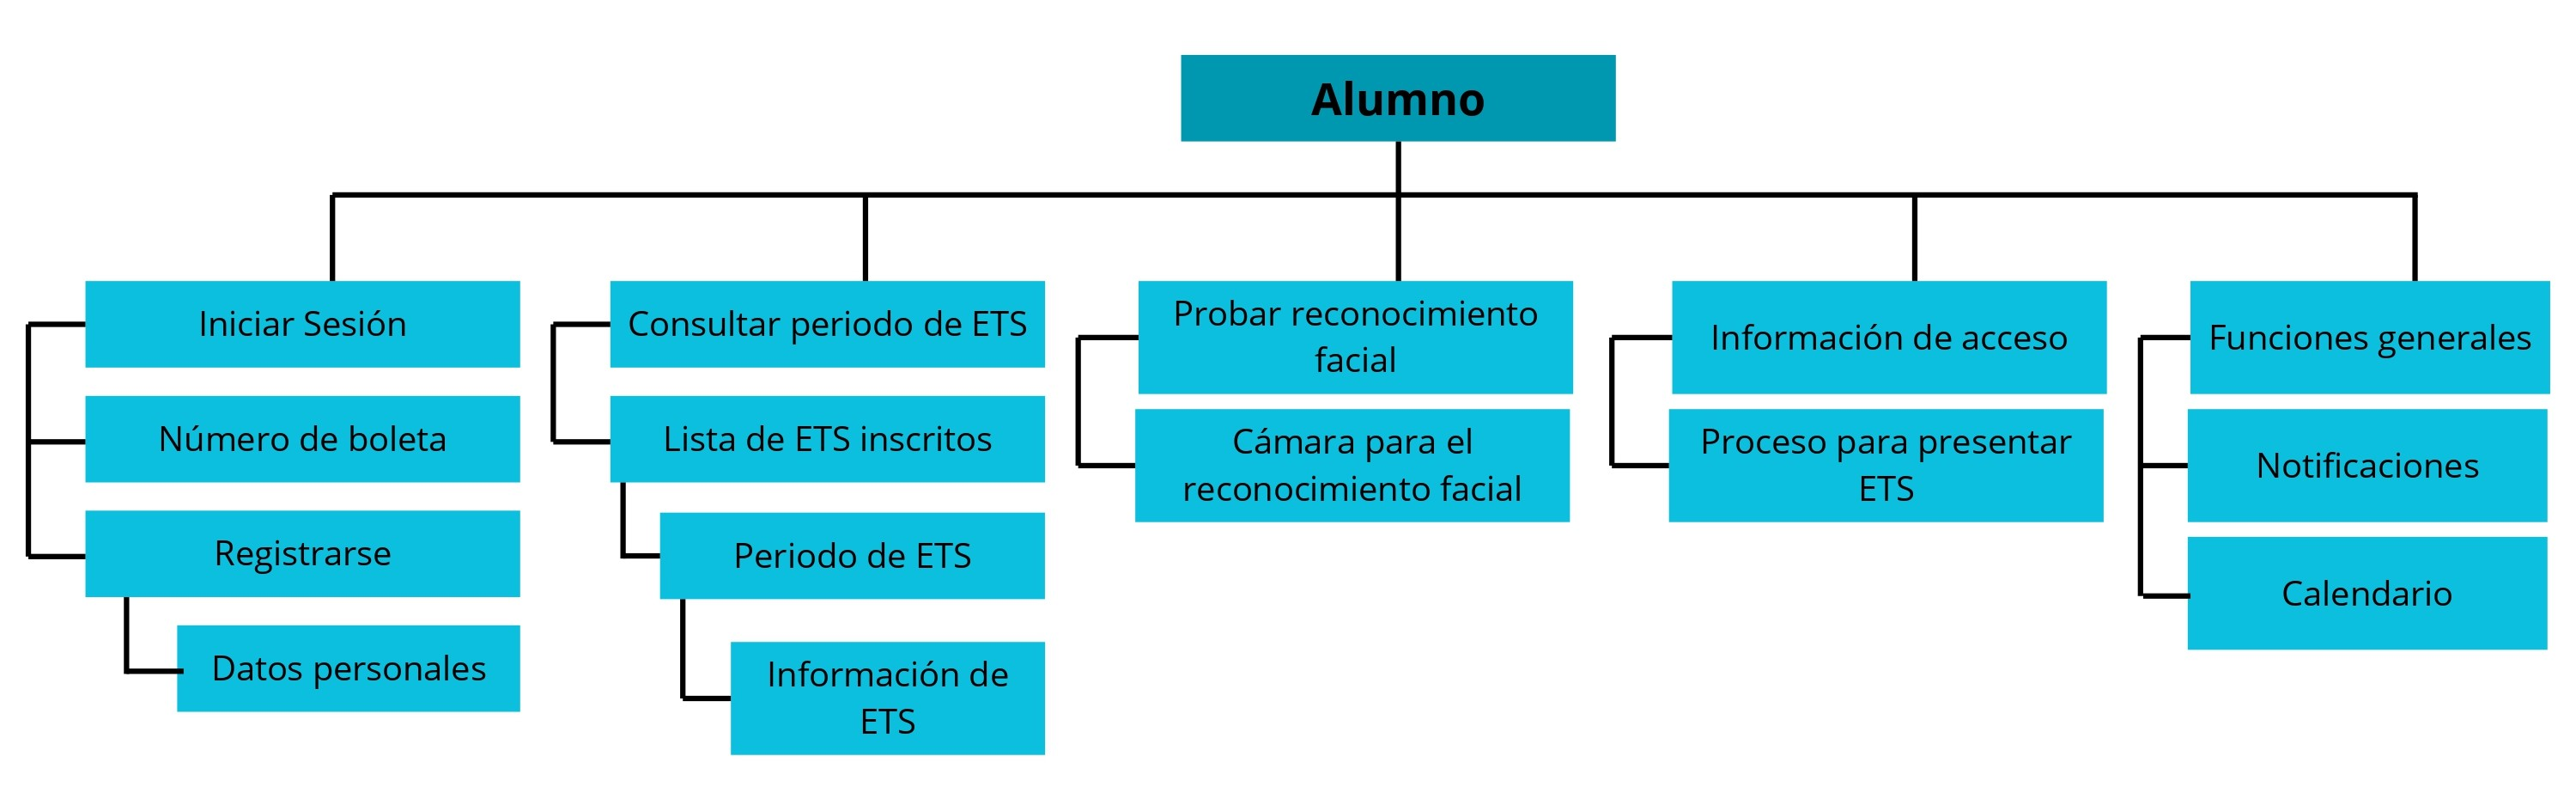
\includegraphics[width=1.0\textwidth]{images/alumno}
			\caption{Mapa de navegación del alumno}
			\label{fig:Mapa de navegación del alumno}
		\end{center}
\end{figure}

\clearpage

\begin{figure}[htbp]
	\begin{center}
		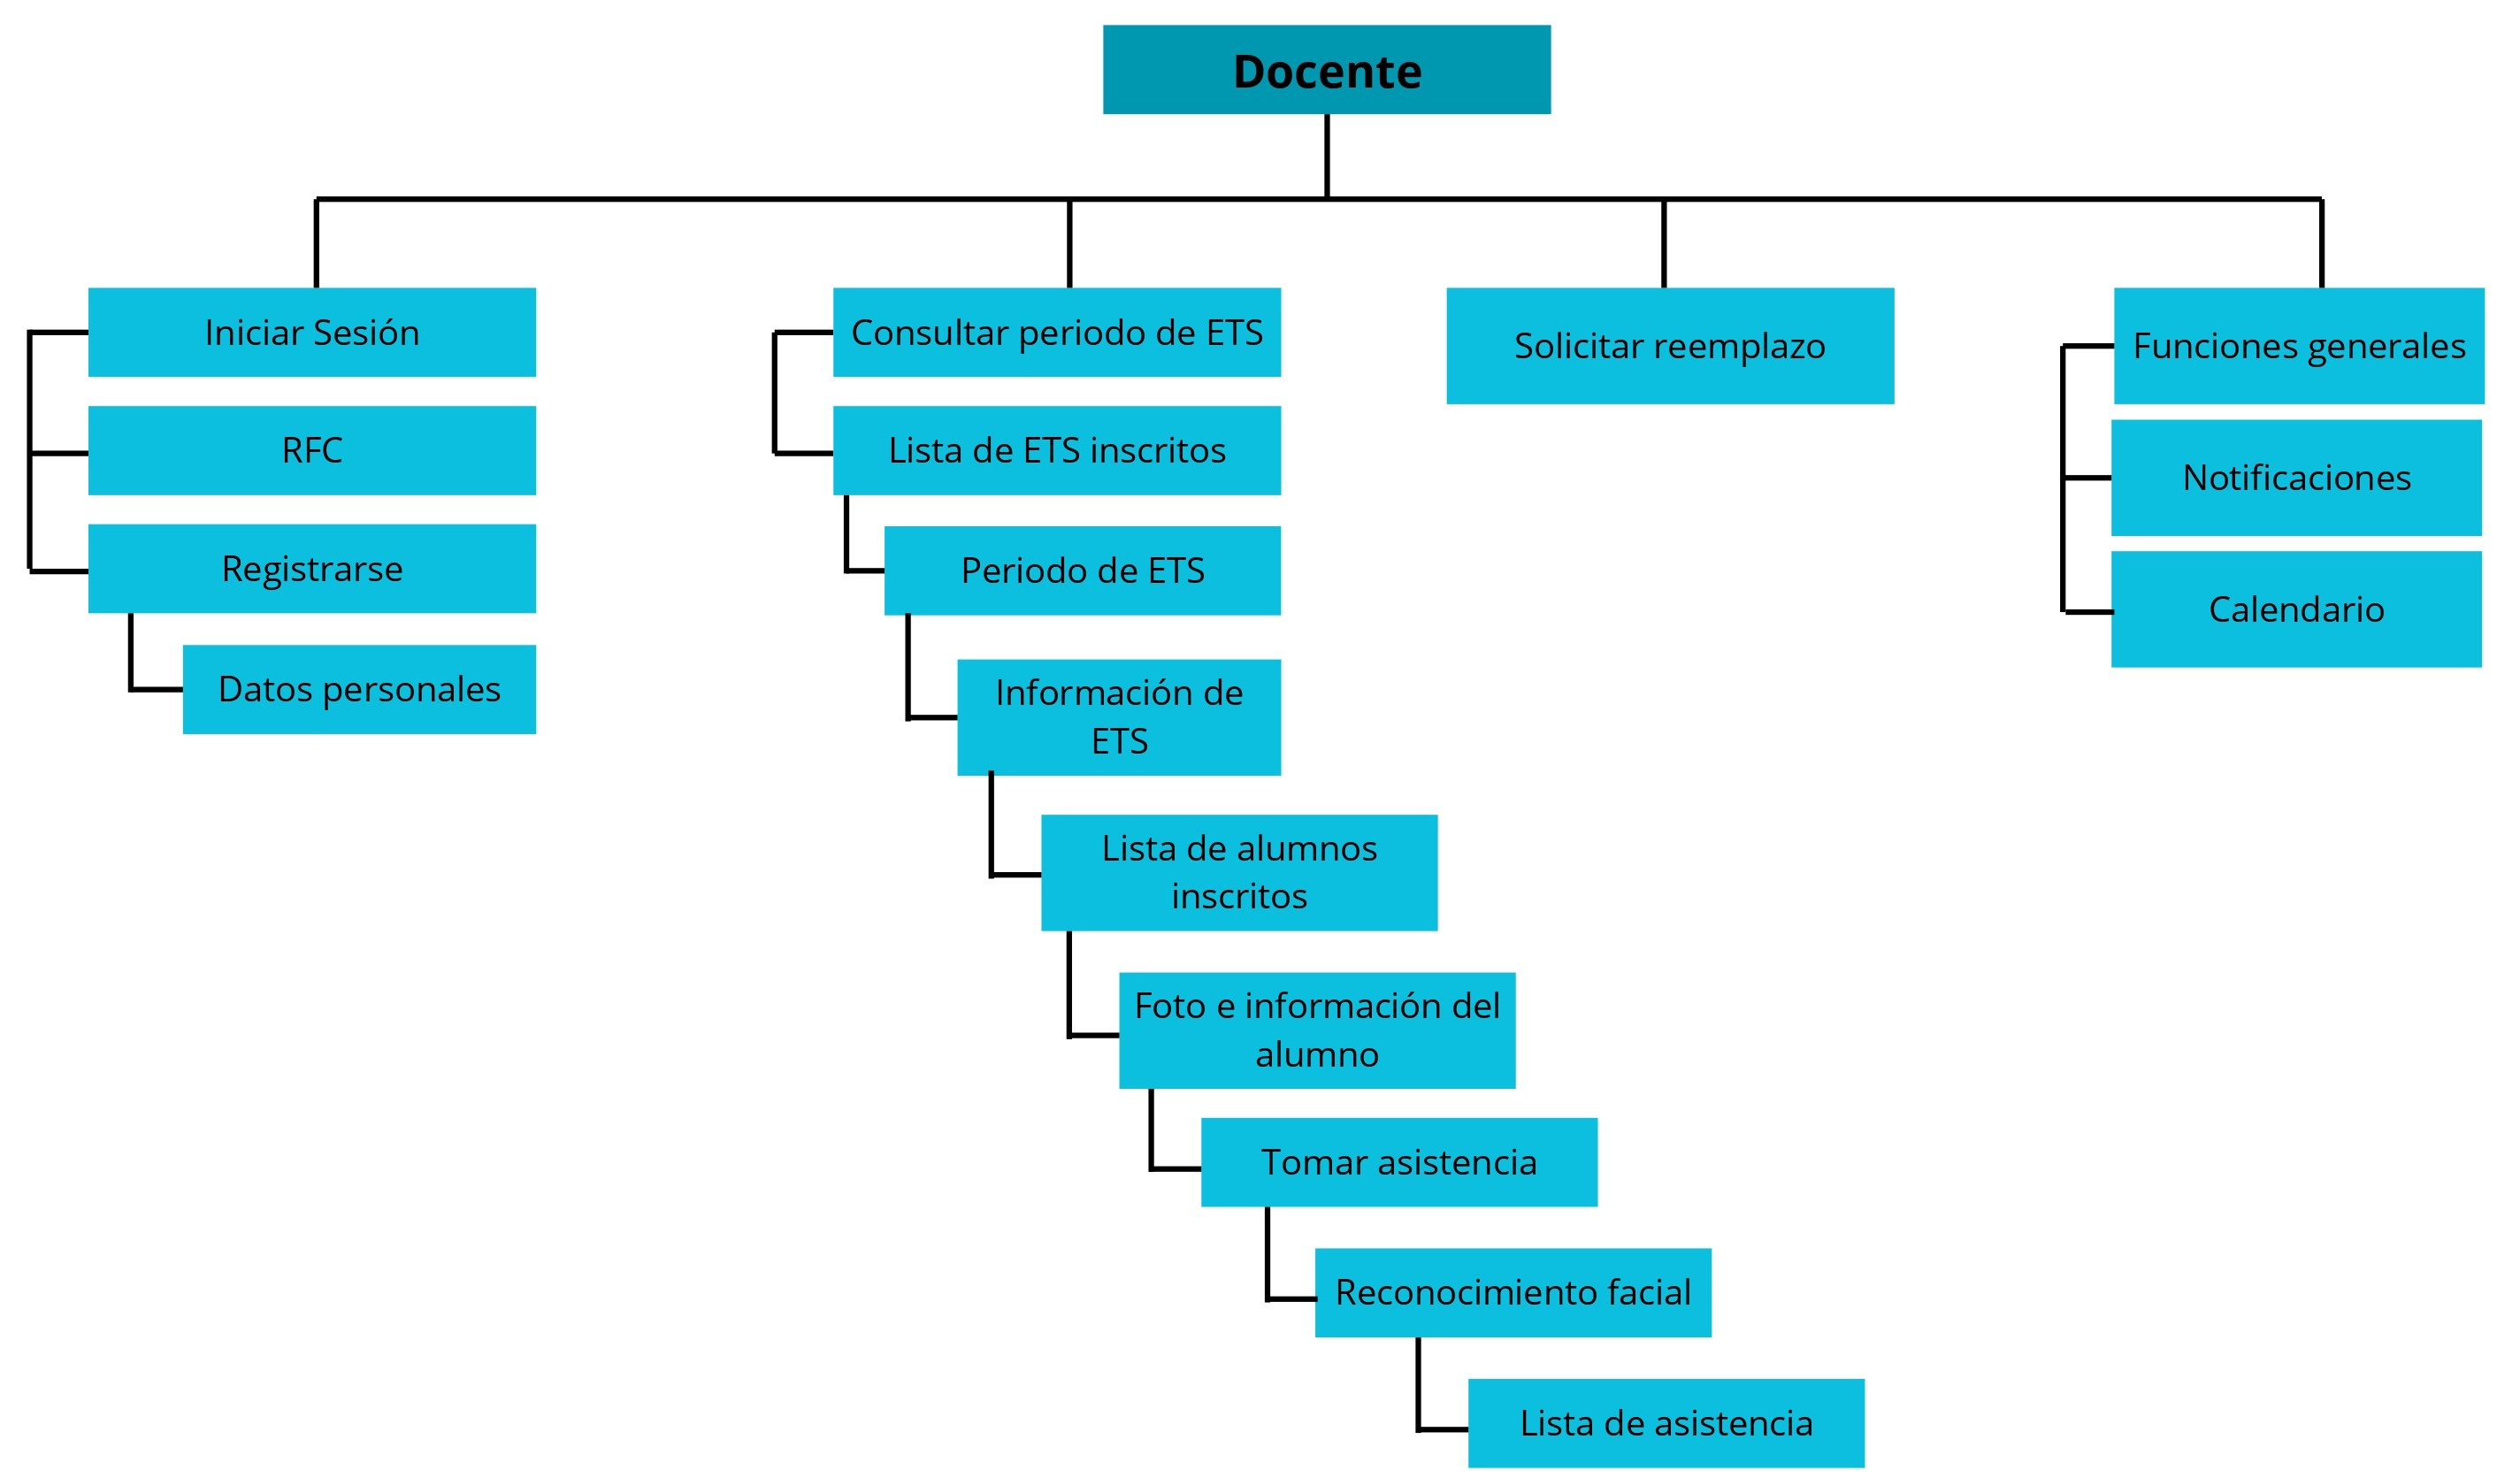
\includegraphics[width=1.0\textwidth]{images/docente}
		\caption{Mapa de navegación del docente}
		\label{fig:Mapa de navegación del docente}
	\end{center}
\end{figure}

\clearpage

\begin{figure}[htbp]
	\begin{center}
		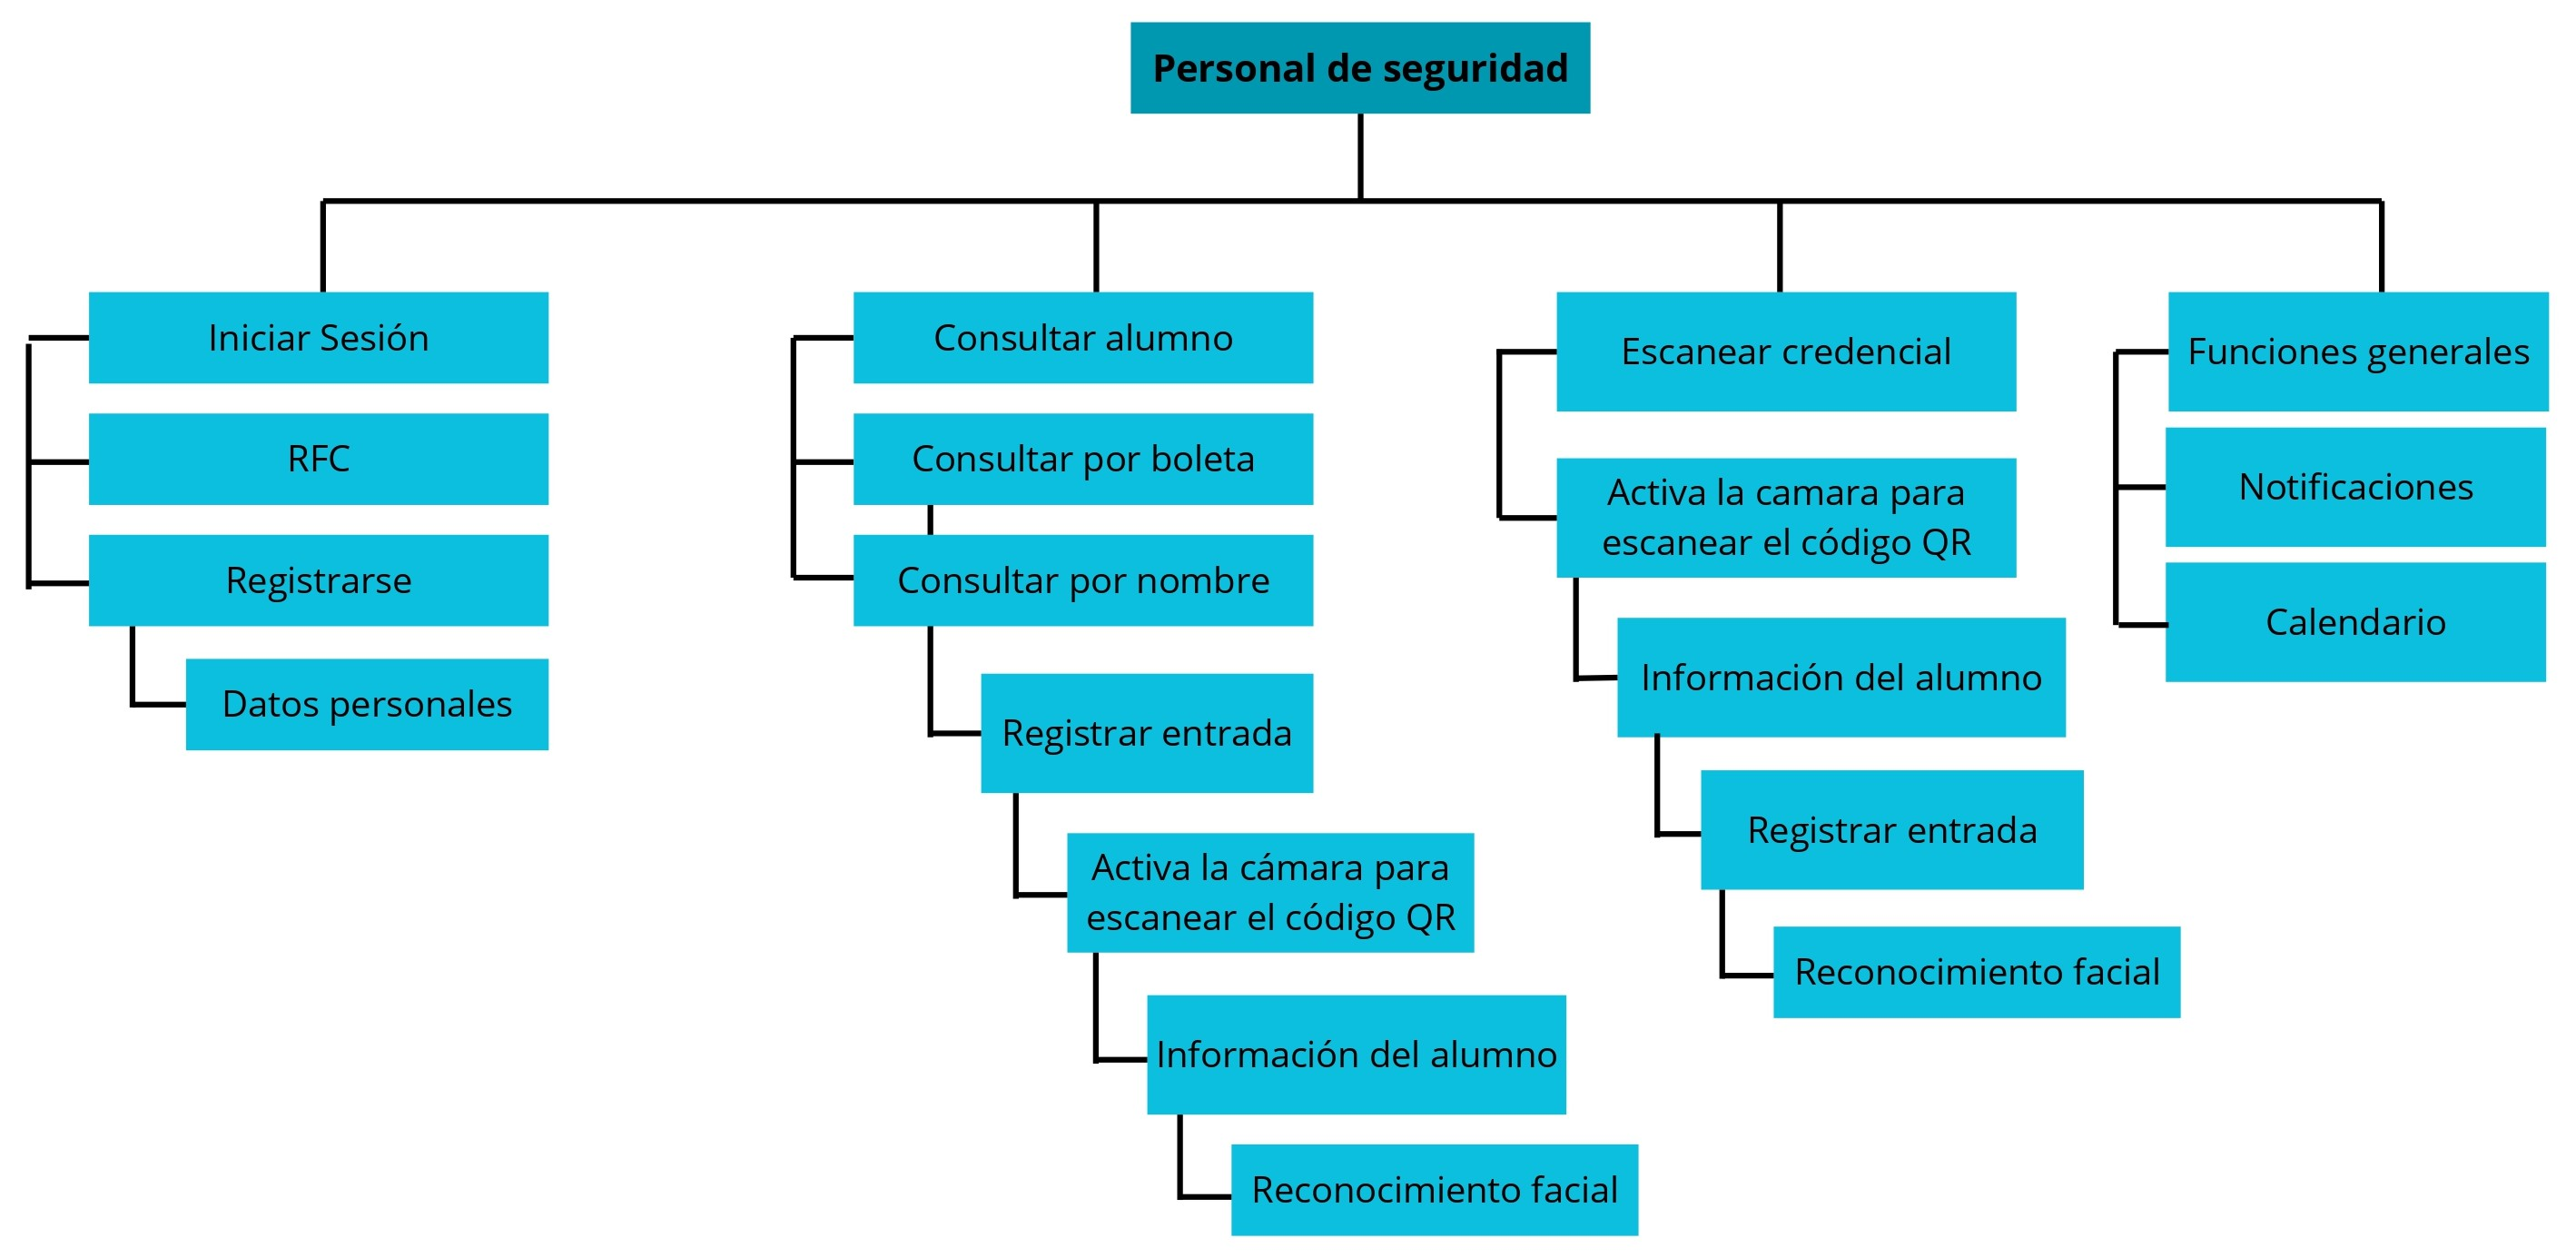
\includegraphics[width=.9\textwidth]{images/personalseguridad}
		\caption{Mapa de navegación del personal de seguridad}
		\label{fig:Mapa de navegación del personal de seguridad}
	\end{center}
\end{figure}

\newpage
% !TeX root = ../ejemplo.tex

%--------------------------------------
\subsection{IU01 Pantalla Iniciar sesión de personal escolar móvil} 

\subsubsection{Objetivo}
	Controlar el acceso al sistema mediante una contraseña a fin de que cada usuario acceda solo a las operaciones permitidas para su perfil.

\subsubsection{Diseño}
	Esta pantalla \IUref{IU01}{Pantalla Iniciar sesión de personal escolar móvil} (ver figura~\ref{IU01}) aparece al iniciar el sistema para los empleados. Para ingresar al mismo se debe escribir el RFC del empleado y la contraseña. 

\IUfig[.35]{UI-CU01}{IU01}{Pantalla Iniciar sesión de personal escolar móvil.}

\subsubsection{Salidas}

Saludo del sistema y mención de su nombre.

\subsubsection{Entradas}
En caso del empleado RFC, Contraseña y en caso del alumno CURP, Contraseña

\subsubsection{Comandos}
\begin{itemize}
	\item \IUbutton{Entrar}: Verifica que el empleado se encuentre registrado y la contraseña sea la correcta. Si la verificación es correcta, se verifica que tipo de empleado y se muestra la pantalla \IUref{IUE01}{Pantalla de Menús de docente} si es docente o \IUref{IUE02}{Pantalla de Menús de personal de seguridad} si es personal de seguridad.
	
	\item \IUbutton{Presiona aquí para pedir su activación}: Redirige a la pantalla \IUref{UI32}{Pantalla de Solicitar desbloqueo de cuenta}
	
\end{itemize}

\subsubsection{Mensajes}

\begin{Citemize}
	\item MSG-1 Los campos no están correctamente llenados. 
	\item MSG-2 Su cuenta esta bloqueada. 
	\item MSG-3 El RFC o la contraseña no corresponden con ningún empleado. 
	\item MSG-4 El proceso no se pudo realizar por un fallo de red. 
	\item MSG-5 Su cuenta ha sido bloqueada por la gran cantidad de intentos de inicio sesión fallidos.
\end{Citemize}


\newpage

% !TeX root = ../ejemplo.tex

%--------------------------------------
\section{IU02 Pantalla Consultar calendario escolar}

\subsection{Objetivo}
Permitir que los usuarios puedan ver el calendario escolar y pedir que se les recuerde cuantos días faltan para que el periodo de ETS comience.
\subsection{Diseño}
    Esta pantalla \IUref{IU02}{Pantalla Consultar calendario escolar} (ver figura~\ref{IU02}) puede ser accedida desde cualquier otra pantalla que no sea el inicio de sesión mediante el botón con forma de calendario.

\IUfig[.35]{UI-CU02}{IU02}{Pantalla Consultar calendario escolar.}

\IUfig[.5]{UI-CU02_2}{IU02-2}{Pantalla Consultar calendario escolar.}

\subsection{Salidas}

    Menciona cuantos días faltan para el periodo de ETS o si menciona que ya es periodo de ETS.

\subsection{Entradas}
   Ninguna.

\subsection{Comandos}
\begin{itemize}
    \item \IUbutton{Calcular cuantos días faltan para el periodo de ETS} toma el día actual y el día de inicio del periodo de ETS más cercano y calcula cuantos días faltan.
    \item \IUbutton{Campana} Redirige a la pantalla \IUref{UI03}{Consultar notificaciones}.
    \item \IUbutton{Home} Redirige a la pantalla de menú correspondiente al tipo de usuario.
\end{itemize}

\subsection{Mensajes}
     
\begin{Citemize}
    \item {\bf MSG7}{``Actualmente es periodo de ETS.''}

    \item {\bf MSG8}{``Actualmente el periodo de ETS no ha sido establecido.''}
\end{Citemize}


\newpage

% !TeX root = ../ejemplo.tex

%--------------------------------------
\section{IU03 Pantalla Consultar notificaciones}

\subsection{Objetivo}
Permitir que los usuarios puedan gestionar sus notificaciones y marcarlas como leidas.
\subsection{Diseño}
    Esta pantalla \IUref{IU03}{Pantalla Consultar notificaciones } (ver figura~\ref{IU03}) puede ser accedida desde cualquier otra pantalla que no sea el inicio de sesión mediante el botón con forma de campana.
\IUfig[.35]{UI-CU03}{IU03}{Pantalla Consultar notificaciones.}

\IUfig[.5]{UI-CU03_2}{IU03-2}{Pantalla Consultar notificaciones.}
\subsection{Salidas}
Menciona que la notificación seleccionada ha sido establecida como leída.
\subsection{Entradas}
   Ninguna.

\subsection{Comandos}
\begin{itemize}
    \item \IUbutton{Botón con palomita} toma la notificación seleccionada y la marca como leída.
    \item \IUbutton{Buscador} En este buscador se puede buscar las notificaciones por fecha.
    \item \IUbutton{Calendario} Redirige a la pantalla \IUref{UI02}{Consultar calendario escolar}
    \item \IUbutton{Home} Redirige a la pantalla de menú correspondiente al tipo de usuario.
\end{itemize}

\subsection{Mensajes}
     
\begin{Citemize}
    \item {\bf MSG9-}{``Actualmente no hay notificaciones.''} 
\end{Citemize}



\newpage

%--------------------------------------
\section{IU04}{Pantalla Periodo de ETS}

\subsection{Objetivo}
	Permitir al docente consultar los periodos de ETS que le han sido asignados. 

\subsection{Diseño}
	Esta pantalla \IUref{IU04}{Pantalla Periodo de ETS} (ver figura~\ref{IU04}) aparece luego de seleccionar la opción de Consultar Periodos de ETS de la pantalla principal. 

\IUfig[.35]{cu04}{IU04}{Pantalla Periodo de ETS.}

\subsection{Salidas}

	Lista de periodos de ETS asignados. 

\subsection{Entradas}
Ninguna

\subsection{Comandos}

\begin{Citemize}
	\item \IUbutton{Calendario} Redirige a la pantalla \IUref{UI02}{Consultar calendario escolar}.
	\item \IUbutton{Campana} Redirige a la pantalla \IUref{UI03}{Consultar notificaciones }.
	\item \IUbutton{Home} Redirige a la pantalla de bienvenida correspondiente al tipo de usuario.
	\item \IUbutton{Periodo de ETS} Selecciona un periodo de ETS y lo redirige a la \IUref{IU04}{pantalla Periodo de ETS}. 
\end{Citemize}


\subsection{Mensajes}

\begin{Citemize}
	\item {\bf MSG-9}{``Error al consultar la base de datos. Intente nuevamente más tarde''.}
	\item {\bf MSG-10}{``No tienes periodos de ETS asignados.''}
\end{Citemize}


\newpage

%--------------------------------------
\section{IU05 Pantalla Consultar ETS}

\subsection{Objetivo}
	Permitir al docente consultar los ETS que tiene asignados. 

\subsection{Diseño}
	Esta pantalla \IUref{IU05}{Pantalla Consultar ETS} (ver figura~\ref{IU05}) aparece luego de seleccionar un periodo de ETS. 

\IUfig[.35]{cu05}{IU05}{Pantalla Consultar ETS.}

\subsection{Salidas}
	Lista de ETS asignados. 

\subsection{Entradas}
	Ninguna
	
\subsection{Comandos}
\begin{Citemize}

	\item \IUbutton{Calendario} Redirige a la pantalla \IUref{UI02}{Consultar calendario escolar}.
	\item \IUbutton{Campana} Redirige a la pantalla \IUref{UI03}{Consultar notificaciones }.
	\item \IUbutton{Home} Redirige a la pantalla de bienvenida correspondiente al tipo de usuario.
	\item \IUbutton{ETS} Selecciona un ETS y lo redirige a la \IUref{IU06}{pantalla Información de ETS}.
\end{Citemize}

\subsection{Mensajes}

\begin{Citemize}
	\item {\bf MSG-9}{``Error al consultar la base de datos. Intente nuevamente más tarde.''.}
	\item {\bf MSG-11}{``No hay ETS asignados actualmente.''}
\end{Citemize}


\newpage

%--------------------------------------
\section{IU06 Pantalla Información de ETS}

\subsection{Objetivo}
	Permitir al docente visualizar la información detallada cada ETS que tiene asignados.
	
\subsection{Diseño}
	Esta pantalla \IUref{IU06}{Pantalla Información de ETS} (ver figura~\ref{IU06}) aparece luego de seleccionar un ETS asignado. 

\IUfig[.35]{cu06}{IU06}{Pantalla Información de ETS}

\subsection{Salidas}

	Información detallada del ETS seleccionado. 

\subsection{Entradas}
Ninguna

\subsection{Comandos}
\begin{itemize}
	\item \IUbutton{Ver alumnos} Redirige a la pantalla \IUref{IU06}{consultar lista de alumnos inscritos a un ETS}
\end{itemize}

\subsection{Mensajes}

\begin{Citemize}
	\item {\bf MSG-12}{``Información no disponible para el ETS seleccionado''}
	\item {\bf MSG-9}{``Error al consultar la base de datos. Intente nuevamente más tarde.''}
\end{Citemize}


\newpage

%--------------------------------------
\section{IU07 Pantalla de Solicitar remplazo}

\subsection{Objetivo}
Permitir al docente pedir que otro docente lo remplaze en la aplicacion de un ETS.

\subsection{Diseño}
Esta pantalla \IUref{IU07}{Pantalla de Solicitar remplazo} (ver figura~\ref{IU07}) aparece luego de que el docente presione el boton \IUbutton{Solicitar docente ayudante} en la pantalla \IUref{IU06}{Pantalla Información de ETS}.

\IUfig[.35]{UI-CU43}{IU07}{Pantalla de Solicitar remplazo}

\subsection{Salidas}
Confirmación de envio de solicitud de remplazo del docente Y y se muestra {\bf MSG-13}{``La notificación ha sido mandada al jefe de departamento y/o al presidente de academia.''}

\subsection{Entradas}
Identificador del ETS y Razon por la que se pide el remplazo.

\subsection{Comandos}
\begin{itemize}
	\item \IUbutton{Enviar}: Permite enviar la notificación al jefe de departamento y/o al presidente de academia para pedir el remplazo.
	\item \IUbutton{Calendario} Redirige a la pantalla \IUref{UI02}{Consultar calendario escolar}.
    \item \IUbutton{Campana} Redirige a la pantalla \IUref{UI03}{Consultar notificaciones }.
    \item \IUbutton{Home} Redirige a la pantalla de bienvenida correspondiente al tipo de usuario.
\end{itemize}

\subsection{Mensajes}

\begin{Citemize}
	\item {\bf MSG-4}{``El proceso no se pudo realizar por un fallo de red.''}
	\item {\bf MSG-13}{``La notificación ha sido mandada al jefe de departamento y/o al presidente de academia.''}
\end{Citemize}


\newpage

%--------------------------------------
\section{IU08 Pantalla Lista de asistencia de ETS}

\subsection{Objetivo}
Permitir al docente visualizar la asistencia de los alumnos inscritos a un ETS asignado.

\subsection{Diseño}
Esta pantalla aparece luego de registrar la asistencia de los alumnos en la \IUref{IU08}{Pantalla lista de asistencia de ETS} (ver figura~\ref{IU08})

\IUfig[.35]{cu08}{IU08}{Pantalla Lista de asistencia de ETS}

\subsection{Salidas}
Lista de asistencia de ETS.

\subsection{Entradas}
Ninguna

\subsection{Comandos}
\begin{itemize}
	\item \IUbutton{Alumno} Selecciona un alumno de la lista para registrar su asistencia y lo redirige a la pantalla \IUref{IU17}{reconocimiento facial}.
	\item \IUbutton{Calendario} Redirige a la pantalla \IUref{UI02}{Consultar calendario escolar}.
    \item \IUbutton{Campana} Redirige a la pantalla \IUref{UI03}{Consultar notificaciones }.
    \item \IUbutton{Home} Redirige a la pantalla de bienvenida correspondiente al tipo de usuario.
\end{itemize}

\subsection{Mensajes}

\begin{Citemize}
	\item {\bf MSG-16}{``No hay alumnos inscritos en este ETS.''}
	\item {\bf MSG-9}{``Error al consultar la base de datos. Intente nuevamente más tarde.''}
	\item {\bf MSG-18}{``Asistencia registrada exitosamente.''}  
\end{Citemize}
\newpage

%--------------------------------------
\subsection{IU09 Asignar docente de remplazo}

\subsubsection{Objetivo}
Permitir al jefe de departamento y/o al presidente de academia responder a las solicitudes de remplazo y asignar un docente de remplazo para el ETS especifico.

\subsubsection{Diseño}
Esta pantalla \IUref{IU09}{Asignar docente de remplazo} (ver figura~\ref{IU09}) aparece luego de que el jefe de departamento y/o al presidente de academia revisen sus notificaciones y seleccione una solicitud de remplazo.

\IUfig[.35]{UI-CU44}{IU09}{Pantalla de Asignar docente de remplazo}

\subsubsection{Salidas}
Confirmación de asignación del nuevo docente y se muestra el mensaje \bf MSG-42{``docente de remplazo asignado con exito.''}.

\subsubsection{Entradas}
Identificador del ETS y nombre del nuevo docente asignado.

\subsubsection{Comandos}
\begin{itemize}
	\item \IUbutton{Asignar}: Permite enviar la notificación docente de que su remplzado ha sido asignado y ademas asigna el remplazo como docente aplicador en el sistema.
\end{itemize}

\subsubsection{Mensajes}

\begin{Citemize}
	\item {\bf MSG-28} {``El proceso no se pudo realizar por un fallo de red''.}
	\item {\bf MSG-42}{``docente de remplazo asignado con exito'.'}
\end{Citemize}



\newpage


%--------------------------------------
\section{IU10 Pantalla Código QR}

\subsection{Objetivo}
Permitir al personal de seguridad escanear el código QR de la credencial del alumno.

\subsection{Diseño}
Esta pantalla \IUref{IU10}{Pantalla Código QR} (ver figura~\ref{IU10}) aparece una vez que el personal de seguridad active la función de escanear credencial del menú. 

\IUfig[.35]{cu12}{IU10}{Pantalla Código QR}

\subsection{Salidas}
Información del alumno

\subsection{Entradas}
Ninguna

\subsection{Comandos}
\begin{itemize}
	\item \IUbutton{Escanear}: Permite escanear el código QR de la credencial del alumno.
	\item \IUbutton{Calendario} Redirige a la pantalla \IUref{UI02}{Consultar calendario escolar}.
    \item \IUbutton{Campana} Redirige a la pantalla \IUref{UI03}{Consultar notificaciones }.
    \item \IUbutton{Home} Redirige a la pantalla de bienvenida correspondiente al tipo de usuario.
\end{itemize}

\subsection{Mensajes}

\begin{Citemize}
	\item {\bf MSG-9}{``Error al consultar la base de datos. Intente nuevamente más tarde.''}.
	\item {\bf MSG-20}{``Alumno no registrado. Verifique el código QR o intente nuevamente.''}
	\item {\bf MSG-19}{``Código QR ilegible. Intente nuevamente.''}
\end{Citemize}


\newpage

%--------------------------------------
\section{IU11}{Pantalla Credencial del alumno}

\subsection{Objetivo}
	Permitir al personal de seguridad consultar la información del alumno mediante el escaneo del código QR de su credencial.

\subsection{Diseño}
Esta pantalla aparece luego de que se escanea el código QR de la credencial del alumno \IUref{IU11}{Pantalla Credencial del alumno} (ver figura~\ref{IU11}).
	

\IUfig[.35]{cu14}{IU11}{Pantalla Credencial del alumno}

\subsection{Salidas}
	Información del alumno

\subsection{Entradas}
Ninguna

\subsection{Comandos}
\begin{itemize}
	\item \IUbutton{Registrar asistencia}: Permite registrar la asistencia del alumno.
	\item \IUbutton{Calendario} Redirige a la pantalla \IUref{UI02}{Consultar calendario escolar}.
    \item \IUbutton{Campana} Redirige a la pantalla \IUref{UI03}{Consultar notificaciones }.
    \item \IUbutton{Home} Redirige a la pantalla de bienvenida correspondiente al tipo de usuario.
\end{itemize}

\subsection{Mensajes}

\begin{Citemize}
	\item {\bf MSG-20}{``Alumno no registrado''}
	\item {\bf MSG-11}{``Error al consultar la base de datos. Intente nuevamente más tarde.''}
\end{Citemize}


\newpage

%--------------------------------------
\section{IU12-1 Pantalla Buscar alumno por boleta}

\subsection{Objetivo}
	Permitir al personal de seguridad buscar la información de un alumno utilizando su numero de boleta. 

\subsection{Diseño}
	Esta pantalla \IUref{IU12}{Pantalla Buscar alumno} (ver figura~\ref{IU12}) aparece luego de seleccionar la opción Consultar alumno. 

\IUfig[.35]{cu11}{IU12}{Pantalla Buscar alumno.}

\subsection{Salidas}
	Información del alumno.

\subsection{Entradas}
Número de boleta del alumno. 

\subsection{Comandos}
Buscador: Permite al usuario buscar al alumno ingresando su numero de boleta. 

\subsection{Mensajes}

\begin{Citemize}
	\item {\bf MSG-20-}{``Alumno no registrado''}
\end{Citemize}


\newpage

%%--------------------------------------
\section{IU12-2 Pantalla Buscar alumno por nombre}

\subsection{Objetivo}
Permitir al personal de seguridad buscar la información de un alumno utilizando su nombre. 

\subsection{Diseño}
Esta pantalla \IUref{IU12}{Pantalla Buscar alumno} aparece luego de seleccionar la opción Consultar alumno. 

\IUfig[.35]{cu11}{IU12}{Pantalla Buscar alumno.}

\subsection{Salidas}
Información del alumno.

\subsection{Entradas}
Nombre del alumno. 

\subsection{Comandos}

\begin{itemize}

	\item Buscador: Permite al usuario buscar al alumno ingresando su nombre. 
	\item \IUbutton{Calendario} Redirige a la pantalla \IUref{UI02}{Consultar calendario escolar}.
    \item \IUbutton{Campana} Redirige a la pantalla \IUref{UI03}{Consultar notificaciones }.
    \item \IUbutton{Home} Redirige a la pantalla de bienvenida correspondiente al tipo de usuario.
\end{itemize}

\subsection{Mensajes}

\begin{Citemize}
	\item {\bf MSG-20}{``Alumno no registrado''}
\end{Citemize}



%\newpage

%--------------------------------------
\subsection{IU13 Pantalla consultar lista de alumnos inscritos a un ETS}

\subsubsection{Objetivo}
Permitir al docente visualizar la lista de los alumnos inscritos a un ETS asignado.

\subsubsection{Diseño}
Esta pantalla aparece luego de seleccionar un ETS en la \IUref{IU13}{Pantalla Informacion de ETS} (ver figura~\ref{IU06} y muestra la boleta, el nombre completo y la foto de los alumnos inscritos al ETS)

\IUfig[.35]{cu07}{IU13}{Consultar lista de alumnos inscritos a un ETS}

\subsubsection{Salidas}
Lista de los alumnos inscritos al ETS.

\subsubsection{Entradas}
Ninguna

\subsubsection{Comandos}
\begin{itemize}
    \item \IUbutton{Calendario} Redirige a la pantalla \IUref{UI02}{Consultar calendario escolar}.
    \item \IUbutton{Campana} Redirige a la pantalla \IUref{UI03}{Consultar notificaciones }.
    \item \IUbutton{Home} Redirige a la pantalla de bienvenida correspondiente al tipo de usuario.
	\item \IUbutton{Tomar asistencia} redirige a la pantalla \IUref{IU08}{Lista de asistencia de ETS}.
\end{itemize}

\subsubsection{Mensajes}

\begin{Citemize}
	\item {\bf MSG-14}{``No hay alumnos inscritos en este ETS.''}
	\item {\bf MSG9-}{``Error al consultar la base de datos. Intente nuevamente más tarde.''}. 
\end{Citemize}
\newpage

%--------------------------------------
\section{IU14} {Pantalla Periodo de ETS del alumno}

\subsection{Objetivo}
	Permitir al alumno consultar los periodos de ETS que le han sido asignados. 

\subsection{Diseño}
	Esta pantalla \IUref{IU14}{Pantalla Periodo de ETS del alumno} (ver figura~\ref{IU14}) aparece luego de seleccionar la opción de Consultar Periodos.

\IUfig[.35]{cu16}{IU14}{Pantalla Periodo de ETS del alumno.}

\subsection{Salidas}
	Lista de periodos de ETS. 

\subsection{Entradas}
Ninguna

\subsection{Comandos}

\begin{itemize}
	\item \IUbutton{Calendario} Redirige a la pantalla \IUref{UI02}{Consultar calendario escolar}.
	\item \IUbutton{Campana} Redirige a la pantalla \IUref{UI03}{Consultar notificaciones }.
	\item \IUbutton{Home} Redirige a la pantalla de bienvenida correspondiente al tipo de usuario.
	\item \IUbutton{Periodo de ETS} Selecciona un periodo de ETS y lo redirige a la pantalla \IUref{UI15}{consultar ETS del alumno}.
\end{itemize}

\subsection{Mensajes}

\begin{Citemize}
	\item {\bf MSG-25}{``No hay periodos de ETS''}
	\item {\bf MSG-9}{``Error al consultar la base de datos. Intente nuevamente más tarde.''}
\end{Citemize}


\newpage

%--------------------------------------
\section{IU15} {Pantalla Consultar ETS del alumno}

\subsection{Objetivo}
Permitir al alumno consultar los ETS que tiene inscritos. 

\subsection{Diseño}
Esta pantalla \IUref{IU15}{Pantalla Consultar ETS del alumno} (ver figura~\ref{IU15}) aparece luego de seleccionar un periodo de ETS. 

\IUfig[.35]{cu17}{IU15}{Pantalla Consultar ETS del alumno.}

\subsection{Salidas}
Lista de ETS asignados. 

\subsection{Entradas}
Ninguna


\subsection{Comandos}

\begin{itemize}
	\item \IUbutton{Calendario} Redirige a la pantalla \IUref{UI02}{Consultar calendario escolar}.
	\item \IUbutton{Campana} Redirige a la pantalla \IUref{UI03}{Consultar notificaciones }.
	\item \IUbutton{Home} Redirige a la pantalla de bienvenida correspondiente al tipo de usuario.
\end{itemize}
\subsection{Mensajes}

\begin{Citemize}
	\item {\bf MSG-26}{``No hay ETS inscritos actualmente.''}
	\item {\bf MSG-09}{``Error al consultar la base de datos. Intente nuevamente más tarde.''}
\end{Citemize}

\newpage

%%--------------------------------------
\section{IU15} {Pantalla Consultar ETS del alumno}

\subsection{Objetivo}
Permitir al alumno consultar los ETS que tiene inscritos. 

\subsection{Diseño}
Esta pantalla \IUref{IU15}{Pantalla Consultar ETS del alumno} (ver figura~\ref{IU15}) aparece luego de seleccionar un periodo de ETS. 

\IUfig[.35]{cu17}{IU15}{Pantalla Consultar ETS del alumno.}

\subsection{Salidas}
Lista de ETS asignados. 

\subsection{Entradas}
Ninguna


\subsection{Comandos}

\begin{itemize}
	\item \IUbutton{Calendario} Redirige a la pantalla \IUref{UI02}{Consultar calendario escolar}.
	\item \IUbutton{Campana} Redirige a la pantalla \IUref{UI03}{Consultar notificaciones }.
	\item \IUbutton{Home} Redirige a la pantalla de bienvenida correspondiente al tipo de usuario.
\end{itemize}
\subsection{Mensajes}

\begin{Citemize}
	\item {\bf MSG-26}{``No hay ETS inscritos actualmente.''}
	\item {\bf MSG-09}{``Error al consultar la base de datos. Intente nuevamente más tarde.''}
\end{Citemize}

%--------------------------------------
\section{IU16 Pantalla Información de ETS}

\subsection{Objetivo}
Permitir al alumno visualizar la información detallada cada ETS que tiene inscrito.

\subsection{Diseño}
Esta pantalla \IUref{IU16}{Pantalla de Información de ETS del alumno} (ver figura~\ref{IU16}) aparece luego de seleccionar un ETS inscrito. 

\IUfig[.35]{cu18}{IU16}{Pantalla de Información de ETS del alumno}

\subsection{Salidas}

Información detallada del ETS seleccionado. 

\subsection{Entradas}
Ninguna


\subsection{Comandos}
\begin{itemize}
	\item \IUbutton{Calendario} Redirige a la pantalla \IUref{UI02}{Consultar calendario escolar}.
    \item \IUbutton{Campana} Redirige a la pantalla \IUref{UI03}{Consultar notificaciones }.
    \item \IUbutton{Home} Redirige a la pantalla de bienvenida correspondiente al tipo de usuario.
\end{itemize}

\subsection{Mensajes}

\begin{Citemize}
	\item {\bf MSG-13}{``Información no disponible para el ETS seleccinado''}
	\item {\bf MSG-11}{``Error al consultar la base de datos. Intente nuevamente más tarde.''}
\end{Citemize}



\newpage

%--------------------------------------
\section{IU17 Pantalla de Reconocimiento facial}

\subsection{Objetivo}
Permitir al docente registrar la asistencia al ETS de los alumnos y al personal de seguridad le permite registrar la entrada a las instalaciones.

\subsection{Diseño}
Esta pantalla \IUref{IU17}{Pantalla de Reconocimiento facial} (ver figura~\ref{IU17}) aparece luego de seleccionar el botón \IUbutton{Registrar asistencia} desde la pantalla \IUref{IU08}{Lista de asistencia de ETS}..


\IUfig[.30]{cu19}{IU17}{Pantalla de Reconocimiento facial}

\subsection{Salidas}
Confirmación de asistencia registrada

\subsection{Entradas}
Ninguna

\subsection{Comandos}
\begin{itemize}
    \item \IUbutton{Cancelar}: Permite al alumno cancelar la operación de Reconocimeinto facial.
    \item \IUbutton{Comenzar}: Activa la cámara para el Reconocimiento facil. 
    \item \IUbutton{Calendario} Redirige a la pantalla \IUref{UI02}{Consultar calendario escolar}.
    \item \IUbutton{Campana} Redirige a la pantalla \IUref{UI03}{Consultar notificaciones }.
    \item \IUbutton{Home} Redirige a la pantalla de bienvenida correspondiente al tipo de usuario.
    \item \IUbutton{Registrar asistencia} Si el usuario que presiona el botón es un docente, marca la asistencia del alumno al ETS, por otro lado si el usuario que presiona es un botón personal de seguridad, marca la entrada del alumno a las instalaciones.
    \item \IUbutton{No registrar asistencia} No marca la asistencia ni la entrada (El alumno no es quien dice ser).
\end{itemize}

\subsection{Mensajes}

\begin{Citemize}
    \item {\bf MSG-17}{``No se pudo activar la cámara o reconocer la identidad. Intente nuevamente.''}
    \item {\bf MSG-16}{``No hay alumnos inscritos en este ETS.''}
    \item {\bf MSG-9}{``Error al consultar la base de datos. Intente nuevamente más tarde.''}
    \item {\bf MSG-15}{``Asistencia registrada exitosamente.''}
    \item {\bf MSG-23}{``Entrada registrada exitosamente.''}
    \item {\bf MSG-24}{``Entrada no registrada .''}
\end{Citemize}

\newpage

%--------------------------------------
\subsection{IU18 Pantalla de Detalles del proceso de ETS}

\subsubsection{Objetivo}
Permitir al alumno visualizar la información detallada sobre el proceso de ETS.

\subsubsection{Diseño}
Esta pantalla \IUref{IU18}{Pantalla de Detalles del proceso de ETS} (ver figura~\ref{IU18}) aparece luego de seleccionar el botón \IUbutton{Revisar Información de acceso}. 

\IUfig[.35]{CU20}{IU18}{Pantalla de Detalles del proces de ETS}

\subsubsection{Salidas}

Información detallada del proceso de ETS. 

\subsubsection{Entradas}
Ninguna


\subsubsection{Comandos}
\begin{itemize}
	\item \IUbutton{Calendario} Redirige a la pantalla \IUref{UI02}{Consultar calendario escolar}.
	\item \IUbutton{Campana} Redirige a la pantalla \IUref{UI03}{Consultar notificaciones }.
	\item \IUbutton{Home} Redirige a la pantalla de bienvenida correspondiente al tipo de usuario.
\end{itemize}
\subsubsection{Mensajes}

\begin{Citemize}
	\item {\bf MSG-9}{``Error al querer mostrar la información. Por favor, intente nuevamente.''}
\end{Citemize}


\newpage

\section{IU19 Pantalla de Reconocimiento facial alumno}

\subsection{Objetivo}
Permitir al alumno probar el reconocimiento facial.

\subsection{Diseño}
Esta pantalla \IUref{IU19}{Pantalla de Reconocimiento facial alumno} (ver figura~\ref{IU19}) aparece luego de seleccionar el botón \IUbutton{Probar reconocimiento facial} en la pantalla \IUref{IU16}{Pantalla de Información de ETS del alumno}.

\IUfig[.35]{cu19-2}{IU19}{Pantalla de Reconocimiento facial}

\subsection{Salidas}
Confirmación de que el reconocimiento facial funciona con el alumno.

\subsection{Entradas}
Ninguna

\subsection{Comandos}
\begin{itemize}
    \item \IUbutton{Cancelar}: Permite al alumno cancelar la operación de Reconocimeinto facial.
    \item \IUbutton{Comenzar}: Activa la cámara para el Reconocimiento facil. 
    \item \IUbutton{Calendario} Redirige a la pantalla \IUref{UI02}{Consultar calendario escolar}.
    \item \IUbutton{Campana} Redirige a la pantalla \IUref{UI03}{Consultar notificaciones }.
    \item \IUbutton{Home} Redirige a la pantalla de bienvenida correspondiente al tipo de usuario.
\end{itemize}

\subsection{Mensajes}

\begin{Citemize}
    \item {\bf MSG-17}{``No se pudo activar la cámara o reconocer la identidad. Intente nuevamente.''}
    \item {\bf MSG-16}{``No hay alumnos inscritos en este ETS.''}
    \item {\bf MSG-9}{``Error al consultar la base de datos. Intente nuevamente más tarde.''}
\end{Citemize}
\newpage

%--------------------------------------
\section{IU20}{Mostrar la foto e información  del alumno}

\subsection{Objetivo}
    Mostrar la al docente la información del alumno seleccionado.

\subsection{Diseño}
    Esta \IUref{IU20}{Pantalla mostrar la foto e información  del alumno} (ver figura~\ref{IU20}) muestra toda la información que necesita al docente para poder reconocerlo.

\IUfig[.35]{cu11}{IU20}{Pantalla mostrar la foto e información  del alumno.}

\subsection{Salidas}

    Ninguna.

\subsection{Entradas}
    Ninguna.

\subsection{Comandos}
\begin{itemize}
    \item \IUbutton{Ampliar fotografía}: Muestra la fotografía del alumno ampliada. 
    
\end{itemize}

\subsection{Mensajes}

\begin{Citemize}
    \item {\bf MSG4-} ``El proceso no se pudo realizar por un falló de red.''
\end{Citemize}


\newpage

% !TeX root = ../ejemplo.tex

%--------------------------------------
\subsection{IU21 Dar de alta a alumno}

\subsubsection{Objetivo}
	Permitir al personal de la DAE dar de alta a un alumno.
\subsubsection{Diseño}
    Esta pantalla \IUref{IU21}{ Dar de alta a alumno } (ver figura~\ref{IU21}) puede ser accedida desde la pantalla \IUref{IUE04}{de personal de la DAE}

\IUfig[1]{UI-CU21}{IU21}{ Dar de alta a alumno.}

\subsubsection{Salidas}
Muestra mensaje {\bf MSG-31} ``Alumno dado de alta con éxito''.
\subsubsection{Entradas}
    \hyperlink{Alumno.Boleta}{Boleta}, \hyperlink{Alumno.Nombre}{Nombre}, \hyperlink{Alumno.CURP}{CURP}, \hyperlink{Alumno.Sexo}{Sexo} y \hyperlink{Alumno.Correo institucional}{Correo institucional}
\subsubsection{Comandos}
\begin{itemize}
    \item \IUbutton{Dar de alta un alumno}  El sistema revisa que los datos del alumno sean válidos, verifica que el CURP o la boleta no hayan sido registrados con anterioridad, mantiene los datos para usarlos en el proceso de crear credencial. Y redirige a la pantalla \IUref{UI22}{Crear credencial}.
    \item \IUbutton{Calendario} Redirige a la pantalla \IUref{UI02}{Consultar calendario escolar}.
    \item \IUbutton{Campana} Redirige a la pantalla \IUref{UI03}{Consultar notificaciones }.
    \item \IUbutton{Home} Redirige a la pantalla de bienvenida correspondiente al tipo de usuario.
    
\end{itemize}

\subsubsection{Mensajes}

\begin{Citemize}
    \item {\bf MSG-31} ``Alumno dado de alta con éxito''.
    \item {\bf MSG-28}  ``El proceso no se pudo realizar por un falló de red.''
    \item {\bf MSG-29}{``Los campos no están correctamente llenados.''}
    \item {\bf MSG-30}{``La CURP o la boleta ya han sido asociadas a este alumno con anterioridad u otro alumno.''}
\end{Citemize}

\newpage

% !TeX root = ../ejemplo.tex

%--------------------------------------
\subsection{IU22 Crear credencial}

\subsubsection{Objetivo}
   Permite al personal de gestión escolar revisar una previsualización de la credencial del alumno y revisar los datos.
\subsubsection{Diseño}
    Esta pantalla \IUref{IU22}{ Crear credencial } (ver figura~\ref{IU22}) puede ser accedida desde la pantalla \IUref{IU21}{ Dar de alta a alumno} apretando el botón \IUbutton{Dar de alta alumno }.

\IUfig[1]{UI-CU22}{IU22}{ Crear credencial.}

\subsubsection{Salidas}
Ninguna
\subsubsection{Entradas}
    \hyperlink{Alumno.Boleta}{Boleta}, \hyperlink{Alumno.Nombre}{Nombre}, \hyperlink{Alumno.CURP}{CURP}, \hyperlink{Alumno.Sexo}{Sexo} y \hyperlink{Alumno.Correo institucional}{Correo institucional}
\subsubsection{Comandos}
\begin{itemize}
\item \IUbutton{Subir foto} Guarda la información y redirige a la pantalla \IUref{UI23}{ Capturar fotografía estudiantil }.
    \item \IUbutton{Home} Redirige a la pantalla de bienvenida correspondiente al tipo de usuario.
    
\end{itemize}

\subsubsection{Mensajes}

\begin{Citemize}
    \item {\bf MSG-28}  ``El proceso no se pudo realizar por un falló de red.''
    \item {\bf MSG-29}{``Los campos no están correctamente llenados.''}
    \item {\bf MSG-30}{``El CURP o la boleta ya han sido asociadas a este alumno con anterioridad u otro alumno.''}
\end{Citemize}

\newpage

% !TeX root = ../ejemplo.tex

%--------------------------------------
\subsection{IU23 Capturar fotografía estudiantil}

\subsubsection{Objetivo}
   Permite agregar una foto a la credencial, para su posterior registro, además de obtener 5 fotos para ser guardadas en la base de datos.
\subsubsection{Diseño}
    Esta pantalla \IUref{IU23}{ Capturar fotografía estudiantil} (ver figura~\ref{IU23}) puede ser accedida desde la pantalla \IUref{IU22}{ Crear credencial} apretando el botón \IUbutton{Subir foto}

\IUfig[1]{UI-CU23}{IU23}{ Capturar fotografía estudiantil.}

\subsubsection{Salidas}
Ninguna
\subsubsection{Entradas}
Ninguna
\subsubsection{Comandos}
\begin{itemize}
    \item \IUbutton{Cámara} Toma 5 fotos al alumno, las cuales guarda en la base de datos para el sistema de reconocimiento facial, de estas la primera la usa para la credencial y redirige a la pantalla \IUref{UI21}{ Capturar fotografía estudiantil }.
    \item \IUbutton{Calendario} Redirige a la pantalla \IUref{UI02}{Consultar calendario escolar}.
    \item \IUbutton{Campana} Redirige a la pantalla \IUref{UI03}{Consultar notificaciones }.
    \item \IUbutton{Home} Redirige a la pantalla de bienvenida correspondiente al tipo de usuario.
    
\end{itemize}

\subsubsection{Mensajes}

\begin{Citemize}
    \item {\bf MSG-28}  ``El proceso no se pudo realizar por un fallo de red.''
\end{Citemize}


\newpage

% !TeX root = ../ejemplo.tex

%--------------------------------------
\section{IU24}{Consultar lista de periodo de ETS}
\subsection{Objetivo}
   Permite al personal de gestión escolar consultar una lista con todos los periodos de ETS y el periodo de ETS más actual en la parte superior.
\subsection{Diseño}
    Esta pantalla \IUref{IU24}{ Consultar lista de periodo de ETS } (ver figura~\ref{IU24}) puede ser accedida desde la pantalla \IUref{IUE05}{de saludo de gestión escolar } apretando el botón \IUbutton{Consultar lista de periodo de ETS}
\IUfig[1]{UI-CU24}{IU24}{ Consultar lista de periodo de ETS.}

\subsection{Salidas}
Ninguna
\subsection{Entradas}
Ninguna
\subsection{Comandos}
\begin{itemize}
    \item \IUbutton{ Dar de alta periodo de ETS } Redirige a la pantalla \IUref{UI25}{ Dar de alta de periodo de ETS}.
    \item \IUbutton{Calendario} Redirige a la pantalla \IUref{UI02}{Consultar calendario escolar}.
    \item \IUbutton{Campana} Redirige a la pantalla \IUref{UI03}{Consultar notificaciones }.
    \item \IUbutton{Home} Redirige a la pantalla de bienvenida correspondiente al tipo de usuario.
    
\end{itemize}

\subsection{Mensajes}

\begin{Citemize}
    \item {\bf MSG-28}  ``El proceso no se pudo realizar por un fallo de red.''
    \item {\bf MSG-31}  ``Ningún periodo de ETS ha sido dado de alta.''
\end{Citemize}



\newpage

% !TeX root = ../ejemplo.tex

%--------------------------------------
\section{IU25 Dar de alta de periodo de ETS}
\subsection{Objetivo}
    Permite al personal de gestión escolar dar de alta un periodo de ETS.
\subsection{Diseño}
    Esta pantalla \IUref{IU25}{Dar de alta de periodo de ETS } (ver figura~\ref{IU25}) puede ser accedida desde la pantalla \IUref{IU24}{Consultar lista de periodo de ETS}
\IUfig[.35]{UI-CU25}{IU25}{Dar de alta de periodo de ETS.}

\subsection{Salidas}
Muestra mensaje {\bf MSG15-} ``Periodo de ETS  dado de alta con éxito''.
\subsection{Entradas}
\hyperlink{Periodo de ETS.Periodo}{Periodo}, \hyperlink{Periodo-de-ETS.Tipo}{Tipo}, \hyperlink{Periodo-de-ETS.Fecha-de-inicio}{Fecha-de-inicio} y \hyperlink{Periodo-de-ETS.Fecha-de-fin}{Fecha-de-fin}
\subsection{Comandos}
\begin{itemize}
    \item \IUbutton{Dar de alta periodo de ETS} Da de alta el nuevo periodo de ETS y redirige a la pantalla \IUref{UI24}{ Consultar lista de periodo de ETS}.
    \item \IUbutton{Calendario} Redirige a la pantalla \IUref{UI02}{Consultar calendario escolar}.
    \item \IUbutton{Campana} Redirige a la pantalla \IUref{UI03}{Consultar notificaciones }.
    \item \IUbutton{Home} Redirige a la pantalla de menú correspondiente al tipo de usuario.
    
\end{itemize}

\subsection{Mensajes}

\begin{Citemize}
    \item {\bf MSG15-} ``Periodo de ETS  dado de alta con éxito''.
    \item {\bf MSG4-}  ``El proceso no se pudo realizar por un fallo de red.''
    \item {\bf MSG1-}{``Los campos no están correctamente llenados.''}
    \item {\bf MSG16-}{`` Periodo, Fecha-de-inicio o Fecha-de-fin ya han sido asociadas a un periodo de ETS.''}
\end{Citemize}


\newpage

% !TeX root = ../ejemplo.tex

%--------------------------------------
\subsection{IU26 Consultar lista de ETS}
\subsubsection{Objetivo}
    Permite al personal de gestión escolar consultar una lista con todos ETS.
\subsubsection{Diseño}
    Esta pantalla \IUref{IU26}{Consultar lista de ETS} (ver figura~\ref{IU26}) puede ser accedida desde la pantalla \IUref{IUE05}{ de saludo de gestión escolar } apretando el botón \IUbutton{Consultar lista de ETS}
\IUfig[]{UI-CU28}{IU26}{Consultar lista ETS.}

\subsubsection{Salidas}
Ninguna
\subsubsection{Entradas}
Ninguna
\subsubsection{Comandos}
\begin{itemize}
    \item \IUbutton{Dar de alta un ETS} Redirige a la pantalla \IUref{UI27}{ Dar de alta ETS}.
    \item \IUbutton{Home} Redirige a la pantalla de bienvenida correspondiente al tipo de usuario.
    
\end{itemize}

\subsubsection{Mensajes}

\begin{Citemize}
    \item {\bf MSG-28}  ``El proceso no se pudo realizar por un fallo de red.''
    \item {\bf MSG-34}  ``Ningún ETS ha sido dado da alta.''
\end{Citemize}


\newpage

% !TeX root = ../ejemplo.tex

%--------------------------------------
\subsection{IU27 Dar de alta ETS}
\subsubsection{Objetivo}
    Permite al personal de gestión escolar dar de alta un ETS.
\subsubsection{Diseño}
    Esta pantalla \IUref{IU27}{Dar de alta ETS} (ver figura~\ref{IU27}) puede ser accedida desde la pantalla \IUref{IU26}{Consultar lista de ETS} apretando el botón \IUbutton{Dar de alta un ETS}
\IUfig[1]{UI-CU29}{IU27}{Dar de alta ETS.}

\subsubsection{Salidas}
Muestra mensaje {\bf MSG-35} ``ETS  dado de alta con éxito''.
\subsubsection{Entradas}
\hyperlink{ETS.ETS }{ETS},  \hyperlink{ETS.Periodo-de-ETS }{ Periodo-de-ETS},  \hyperlink{ETS.Fecha}{Fecha},  \hyperlink{ETS.Turno}{Turno},  \hyperlink{ETS.Cupo} {Cupo} ,  \hyperlink{ETS.Unidad-de-aprendizaje }{Unidad-de-aprendizaje},  \hyperlink{ETS.Salon}{Salon} y \hyperlink{ETS.Docente}{Docente} .
\subsubsection{Comandos}
\begin{itemize}
    \item \IUbutton{Dar de alta ETS} Da de alta el nuevo ETS y redirige a la pantalla \IUref{UI26}{Consultar lista de ETS}.
    \item \IUbutton{Home} Redirige a la pantalla de bienvenida correspondiente al tipo de usuario.
    
\end{itemize}

\subsubsection{Mensajes}

\begin{Citemize}
    \item {\bf MSG-35} ``ETS  dado de alta con éxito''.
    \item {\bf MSG-28}  ``El proceso no se pudo realizar por un fallo de red.''
    \item {\bf MSG-29}{``Los campos no están correctamente llenados.''}
    \item {\bf MSG-36}{`` ETS o salón  ya han sido asociadas a un ETS de ETS.''}
    
\end{Citemize}


\newpage

% !TeX root = ../ejemplo.tex

%--------------------------------------
\section{IU32 Consultar lista de personal de seguridad}
\subsection{Objetivo}
   Permite al personal de gestión escolar consultar una lista con todo el personal de seguridad.
\subsection{Diseño}
    Esta pantalla \IUref{IU32}{Consultar lista de personal de seguridad} (ver figura~\ref{IU32}) puede ser accedida desde la pantalla \IUref{IUE05}{ Menú de personal de gestión escolar }
\IUfig[.35]{UI-CU32}{IU32}{Consultar lista de personal de seguridad}

\subsection{Salidas}
Ninguna
\subsection{Entradas}
Ninguna
\subsection{Comandos}
\begin{itemize}
    \item \IUbutton{Dar de alta personal de seguridad} Redirige a la pantalla \IUref{UI33}{Dar de alta personal de seguridad}.
    \item \IUbutton{Calendario} Redirige a la pantalla \IUref{UI02}{Consultar calendario escolar}.
    \item \IUbutton{Campana} Redirige a la pantalla \IUref{UI03}{Consultar notificaciones }.
    \item \IUbutton{Home} Redirige a la pantalla de menú correspondiente al tipo de usuario.
    
\end{itemize}

\subsection{Mensajes}

\begin{Citemize}
    \item {\bf MSG4-}  ``El proceso no se pudo realizar por un fallo de red.''
    \item {\bf MSG13-}  ``No hay personal de seguridad dado de alta.''
    
\end{Citemize}



\newpage

% !TeX root = ../ejemplo.tex

%--------------------------------------
\section{IU33 Dar de alta personal de seguridad}
\subsection{Objetivo}
    Permite al personal de gestión escolar dar de alta a personal de seguridad.
\subsection{Diseño}
    Esta pantalla \IUref{IU33}{Dar de alta personal de seguridad} (ver figura~\ref{IU33}) puede ser accedida desde la pantalla \IUref{IU32}{Consultar lista de personal de seguridad}
\IUfig[.35]{UI-CU33}{IU33}{Dar de alta personal de seguridad.}

\subsection{Salidas}
Muestra mensaje {\bf MSG19-} ``Personal de seguridad dado de alta con éxito''.
\subsection{Entradas}
\hyperlink{Personal-de-seguridad.CURP }{CURP}, \hyperlink{personal-de-seguridad.Turno }{Turno }, \hyperlink{ Personal-de-seguridad.Cargo }{Cargo}, \hyperlink{ Personal-de-seguridad.Sexo}{Sexo} y \hyperlink{ Personal-de-seguridad.Nombre}{Nombre} 
\subsection{Comandos}
\begin{itemize}
    \item \IUbutton{Dar de alta personal de seguridad} Da de alta el nuevo personal de seguridad y redirige a la pantalla \IUref{UI32}{Consultar lista de personal de seguridad}.
    \item \IUbutton{Calendario} Redirige a la pantalla \IUref{UI02}{Consultar calendario escolar}.
    \item \IUbutton{Campana} Redirige a la pantalla \IUref{UI03}{Consultar notificaciones }.
    \item \IUbutton{Home} Redirige a la pantalla de menú correspondiente al tipo de usuario.
    
\end{itemize}

\subsection{Mensajes}

\begin{Citemize}
    \item {\bf MSG19-} ``Personal de seguridad dado de alta con éxito''.
    \item {\bf MSG4-}  ``El proceso no se pudo realizar por un fallo de red.''
    \item {\bf MSG1-}{``Los campos no están correctamente llenados.''}
    \item {\bf MSG20-}{``El CURP ya ha sido asociado a este personal de seguridad con anterioridad u otro personal de seguridad.''}
    
\end{Citemize}

\newpage

% !TeX root = ../ejemplo.tex

%--------------------------------------
\section{IU30}{Consultar lista de docentes}
\subsection{Objetivo}
   Permite al personal de gestión escolar consultar una lista con todos los docentes dados de alta.
\subsection{Diseño}
    Esta pantalla \IUref{IU30}{Consultar lista de docentes} (ver figura~\ref{IU30}) puede ser accedida desde la pantalla \IUref{IUE05}{de saludo de personal de gestión escolar } apretando el botón \IUbutton{Consultar lista de docentes}.
\IUfig[1]{UI-CU36}{IU30}{Consultar lista de docentes.}

\subsection{Salidas}
Ninguna
\subsection{Entradas}
Ninguna
\subsection{Comandos}
\begin{itemize}
    \item \IUbutton{Dar de alta docente} Redirige a la pantalla \IUref{UI31}{Dar de alta docente}.
    \item \IUbutton{Calendario} Redirige a la pantalla \IUref{UI02}{Consultar calendario escolar}.
    \item \IUbutton{Campana} Redirige a la pantalla \IUref{UI03}{Consultar notificaciones }.
    \item \IUbutton{Home} Redirige a la pantalla de bienvenida correspondiente al tipo de usuario.
    
\end{itemize}

\subsection{Mensajes}

\begin{Citemize}
    \item {\bf MSG-28}  ``El proceso no se pudo realizar por un fallo de red.''
    \item {\bf MSG-39}  ``No hay docentes dados de alta.''
\end{Citemize}



\newpage

% !TeX root = ../ejemplo.tex

%--------------------------------------
\section{IU31}{Dar de alta docente}
\subsection{Objetivo}
    Permite al personal de gestión escolar dar de alta nuevos docentes.
\subsection{Diseño}
    Esta pantalla \IUref{IU31}{Dar de alta docente} (ver figura~\ref{IU31}) puede ser accedida desde la pantalla \IUref{IU30}{Consultar lista de docentes} apretando el botón \IUbutton{Dar de alta docente}.
\IUfig[1]{UI-CU37}{IU31}{Dar de alta docente}

\subsection{Salidas}
Muestra mensaje {\bf MSG-41} ``Docente dado de alta con éxito''.
\subsection{Entradas}
\hyperlink{Docente.CURP }{CURP}, \hyperlink{Docente.RFC }{RFC }, \hyperlink{Docente.Correo-institucional}{ Correo-institucional }, \hyperlink{Docente.Sexo}{Sexo}, \hyperlink{ Docente.Nombre}{Nombre} y \hyperlink{Docente.Cargo}{Cargo}
\subsection{Comandos}
\begin{itemize}
    \item \IUbutton{Dar de alta docente} Da de alta al nuevo docente y redirige a la pantalla \IUref{UI30}{Consultar lista de docentes}.
    \item \IUbutton{Calendario} Redirige a la pantalla \IUref{UI02}{Consultar calendario escolar}.
    \item \IUbutton{Campana} Redirige a la pantalla \IUref{UI03}{Consultar notificaciones }.
    \item \IUbutton{Home} Redirige a la pantalla de bienvenida correspondiente al tipo de usuario.
    
\end{itemize}

\subsection{Mensajes}

\begin{Citemize}
    \item {\bf MSG-41} ``Docente dado de alta con éxito''.
    \item {\bf MSG-28}  ``El proceso no se pudo realizar por un fallo de red.''
    \item {\bf MSG-29}{``Los campos no están correctamente llenados.''}
    \item {\bf MSG-40}{``El CURP o el RFC ya ha sido asociado a este docente con anterioridad u otro docente.''}
\end{Citemize}


\newpage

% !TeX root = ../ejemplo.tex

%--------------------------------------
\subsection{IU32 Iniciar Solicitar desbloqueo de cuenta}

\subsubsection{Objetivo}
    Mandar una petición de desbloqueo de cuenta mediante correo electrónico.

\subsubsection{Diseño}
	Esta pantalla \IUref{IU32}{Pantalla Solicitar desbloqueo de cuenta} (ver figura~\ref{IU32}) puede ser accedida desde cualquier desde cualquier inicio de sesion.

\IUfig[.35]{UI-CU40}{IU32}{Pantalla Solicitar desbloqueo de cuenta.}

\IUfig[1]{UI-CU40_2}{IU32-2}{Pantalla Solicitar desbloqueo de cuenta.}

\subsubsection{Salidas}

    Manda un correo electrónico con una cuenta default con los datos requeridos para solicitar la reactivación de su cuenta.

\subsubsection{Entradas}
    Una justificación de la causa del bloqueo, para el alumno \hyperlink{Alumno.Boleta}{Boleta} y para el resto de usuarios \hyperlink{Empleado.RFC}{RFC}.


\subsubsection{Comandos}
\begin{itemize}

    \item \IUbutton{Enviar} Envía un correo electrónico con una cuenta default con los datos requeridos para solicitar la reactivación de su cuenta
    \item \IUbutton{Calendario} Redirige a la pantalla \IUref{UI02}{Consultar calendario escolar}.
    \item \IUbutton{Campana} Redirige a la pantalla \IUref{UI03}{Consultar notificaciones }.
    \item \IUbutton{Home} Redirige a la pantalla de menú correspondiente al tipo de usuario.
	
\end{itemize}

\subsubsection{Mensajes}

\begin{Citemize}
	\item {\bf MSG1-}{``Los campos no están correctamente llenados.''}
	\item {\bf MSG4-}  ``El proceso no se pudo realizar por un fallo de red.''
	\item {\bf MSG10-}  ``Los datos no coinciden con ningún usuario''.
\end{Citemize}

\newpage

%--------------------------------------
\subsection{IU33 Pantalla Iniciar sesión de personal escolar web}

\subsubsection{Objetivo}
	Controlar el acceso al sistema mediante una contraseña a fin de que cada usuario acceda solo a las operaciones permitidas para su perfil.

\subsubsection{Diseño}
	Esta pantalla \IUref{IU33}{Pantalla iniciar sesión de personal escolar web} (ver figura~\ref{IU33}) aparece al iniciar el sistema para los empleados. Para ingresar al mismo se debe escribir el RFC del empleado y la contraseña. 

\IUfig[1]{UI-CU41}{IU33}{Pantalla Iniciar sesión de personal escolar web.}

\subsubsection{Salidas}

	Ninguna.

\subsubsection{Entradas}
	RFC y contraseña del empleado.

\subsubsection{Comandos}
\begin{itemize}
	\item \IUbutton{Entrar}: Verifica que el empleado se encuentre registrado y la contraseña sea la correcta. Si la verificación es correcta, se verifica que tipo de empleado y se muestra la pantalla \IUref{IUE04}{Pantalla de saludo de personal de la DAE} si es personal de la DAE Y \IUref{IUE05}{Pantalla de saludo de personal de gestión escolar} si es personal de gestión escolar.
	
	\item \IUbutton{Presiona aquí para pedir su activación}: Redirige a la pantalla \IUref{UI32}{Pantalla de Solicitar desbloqueo de cuenta}
	
\end{itemize}

\subsubsection{Mensajes}

\begin{Citemize}
	\item MSG-1 Los campos no están correctamente llenados. 
	\item MSG-2 Su cuenta esta bloqueada. 
	\item MSG-3 El RFC o la contraseña no corresponden con ningún empleado. 
	\item MSG-4 El proceso no se pudo realizar por un fallo de red. 
	\item MSG-5 Su cuenta ha sido bloqueada por la gran cantidad de intentos de inicio sesión fallidos.
\end{Citemize}


\newpage


% !TeX root = ../ejemplo.tex
%--------------------------------------
\subsection{IUE01 Saludo de docente}

\subsubsection{Objetivo}
	Mostrar una pantalla de home después de iniciar sesión y marcar las acciones que el docente puede hacer.

\subsubsection{Diseño}
	Esta pantalla \IUref{IUE01}{Pantalla saludo de docente} (ver figura~\ref{IUE01}) aparece al iniciar sesión exitosamente y muestra las acciones que el docente puede hacer,ademas de las opciones generales de usuario (Consultar calendario escolar y consultar notificaciones). 

\IUfig[.35]{IUE01}{IUE01}{Pantalla Menú de docente.}

\subsubsection{Salidas}

	Ninguna.

\subsubsection{Entradas}
	Ninguna.

\subsubsection{Comandos}
\begin{itemize}
	\item \IUbutton{Consultar periodos de ETS asignados}: Redirige a los docentes a la pantalla \IUref{IU04}{Consultar periodos de ETS asignados al docente}
	\item \IUbutton{Notificaciones}: Redirige a los docentes a la pantalla \IUref{IU03}{Consultar notificaciones}
	\item \IUbutton{Calendario}: Redirige a los docentes a la pantalla \IUref{IU02}{Consultar calendario escolar}
	
\end{itemize}

\subsubsection{Mensajes}

\begin{Citemize}
	\item Ninguno.
\end{Citemize}


\newpage

% !TeX root = ../ejemplo.tex
%--------------------------------------
\section{IUE02 saludo de personal de seguridad}

\subsection{Objetivo}
Mostrar una pantalla de home después de iniciar sesión y marcar las acciones que el personal de seguridad puede hacer.

\subsection{Diseño}
Esta pantalla \IUref{IUE02}{Pantalla saludo de personal de seguridad} (ver figura~\ref{IUE02}) aparece al iniciar sesión exitosamente y muestra las acciones que el personal de seguridad puede hacer,ademas de las opciones generales de usuario (Consultar calendario escolar y consultar notificaciones). 

\IUfig[.35]{IUE02}{IUE02}{Pantalla Menú de personal de seguridad.}

\subsection{Salidas}

Ninguna.

\subsection{Entradas}
Ninguna.

\subsection{Comandos}
\begin{itemize}
	\item \IUbutton{Consultar alumno}: Redirige a el personal de seguridad a la pantalla \IUref{IU12}{Buscar alumno}.
	
	\item \IUbutton{Escanear credencial}: Redirige a el personal de seguridad a la pantalla \IUref{IU10}{Pantalla código QR}.
	
	\item \IUbutton{Notificaciones}: Redirige a el personal de seguridad la pantalla \IUref{IU03}{Consultar notificaciones}
	
	\item \IUbutton{Calendario}: Redirige a el personal de seguridad a la pantalla \IUref{IU02}{Consultar calendario escolar}
	
\end{itemize}

\subsection{Mensajes}

\begin{Citemize}
	\item Ninguno.
\end{Citemize}


\newpage

% !TeX root = ../ejemplo.tex
%--------------------------------------
\subsection{IUE03 saludo de alumno}

\subsubsection{Objetivo}
Mostrar una pantalla de home después de iniciar sesión y marcar las acciones que el alumno puede hacer.

\subsubsection{Diseño}
Esta pantalla \IUref{IUE03}{Pantalla saludo de alumno} (ver figura~\ref{IUE03}) aparece al iniciar sesión exitosamente y muestra las acciones que el alumno puede hacer,ademas de las opciones generales de usuario (Consultar calendario escolar y consultar notificaciones). 

\IUfig[.35]{IUE03}{IUE03}{Pantalla saludo de alumno.}

\subsubsection{Salidas}

Ninguna.

\subsubsection{Entradas}
Ninguna.

\subsubsection{Comandos}
\begin{itemize}
	\item \IUbutton{Consultar periodos de ETS asignados}: Redirige a los alumnos a la pantalla \IUref{IU13}{Consultar periodo de ETS de alumnos}
	\item \IUbutton{Información de acceso}: Redirige a los alumnos a la pantalla \IUref{IU18}{Consultar periodo de ETS de alumnos}
	\item \IUbutton{Notificaciones}: Redirige a los alumnos a la pantalla \IUref{IU03}{Consultar notificaciones}
	\item \IUbutton{Calendario}: Redirige a los alumnos a la pantalla \IUref{IU02}{Consultar calendario escolar}
	
\end{itemize}

\subsubsection{Mensajes}

\begin{Citemize}
	\item Ninguno.
\end{Citemize}


\newpage

% !TeX root = ../ejemplo.tex
%--------------------------------------
\section{IUE04 saludo de personal de la DAE}

\subsection{Objetivo}
Mostrar una pantalla de home después de iniciar sesión y marcar las acciones que el personal de la DAE puede hacer.

\subsection{Diseño}
Esta pantalla \IUref{IUE04}{Pantalla saludo de personal de la DAE} (ver figura~\ref{IUE04}) aparece al iniciar sesión exitosamente y muestra las acciones que el personal de la DAE puede hacer,ademas de las opciones generales de usuario (Consultar calendario escolar y consultar notificaciones). 

\IUfig[1]{IUE04}{IUE04}{Pantalla saludo de personal de la DAE.}

\subsection{Salidas}

Ninguna.

\subsection{Entradas}
Ninguna.

\subsection{Comandos}
\begin{itemize}
	\item \IUbutton{Consultar periodos de ETS asignados}: Redirige al personal de la DAE a la pantalla \IUref{IU21}{Dar de alta a los estudiantes}
	\item \IUbutton{Notificaciones}: Redirige al personal de la DAE a la pantalla \IUref{IU03}{Consultar notificaciones}
	\item \IUbutton{Calendario}: Redirige al personal de la DAE a la pantalla \IUref{IU02}{Consultar calendario escolar}
	
\end{itemize}

\subsection{Mensajes}

\begin{Citemize}
	\item Ninguno.
\end{Citemize}


\newpage

% !TeX root = ../ejemplo.tex
%--------------------------------------
\subsection{IUE05 saludo de personal de gestión escolar}

\subsubsection{Objetivo}
Mostrar una pantalla de home después de iniciar sesión y marcar las acciones que el personal de gestión escolar puede hacer.

\subsubsection{Diseño}
Esta pantalla \IUref{IUE05}{Pantalla saludo de personal de gestión escolar} (ver figura~\ref{IUE05}) aparece al iniciar sesión exitosamente y muestra las acciones que el personal de gestión escolar puede hacer,ademas de las opciones generales de usuario (Consultar calendario escolar y consultar notificaciones). 

\IUfig[1]{IUE05}{IUE05}{Pantalla saludo de personal de gestión escolar.}

\subsubsection{Salidas}

Ninguna.

\subsubsection{Entradas}
Ninguna.

\subsubsection{Comandos}
\begin{itemize}
	\item \IUbutton{Consultar lista de periodo de ETS}: Redirige al personal de gestión escolar a la pantalla \IUref{IU24}{Consultar lista de periodo de ETS}
	\item \IUbutton{Consultar lista de ETS}: Redirige al personal de gestión escolar a la pantalla \IUref{IU26}{Consultar lista de ETS}
	\item \IUbutton{Consultar lista de personal de seguridad}: Redirige al personal de gestión escolar a la pantalla \IUref{IU28}{Consultar lista de personal de seguridad}
	\item \IUbutton{Consultar lista de docentes}: Redirige al personal de gestión escolar a la pantalla \IUref{IU30}{Consultar lista de docentes}
	\item \IUbutton{Notificaciones}: Redirige al personal de gestión escolar a la pantalla \IUref{IU03}{Consultar notificaciones}
	\item \IUbutton{Calendario}: Redirige al personal de gestión escolar a la pantalla \IUref{IU02}{Consultar calendario escolar}
	
\end{itemize}

\subsubsection{Mensajes}

\begin{Citemize}
	\item Ninguno.
\end{Citemize}


\newpage

% !TeX root = ../ejemplo.tex
%--------------------------------------
\subsection{IUE06 saludo del presidente de academia y el jefe de departamento}

\subsubsection{Objetivo}
Mostrar una pantalla de home después de iniciar sesión y marcar las acciones que el presidente de academia y el jefe de departamento pueden hacer.

\subsubsection{Diseño}
Esta pantalla \IUref{IUE06}{saludo del presidente de academia y el jefe de departamento} (ver figura~\ref{IUE06}) aparece al iniciar sesión exitosamente y muestra las acciones que el presidente de academia y el jefe de departamento pueden hacer,ademas de las opciones generales de usuario (Consultar calendario escolar y consultar notificaciones). 

\IUfig[0.3]{IUE06}{IUE06}{saludo del presidente de academia y el jefe de departamento.}

\subsubsection{Salidas}
 
Ninguna.

\subsubsection{Entradas}
Ninguna.

\subsubsection{Comandos}
\begin{itemize}
	\item \IUbutton{Asignar docente de remplazo }: Redirige al presidente de academia y al jefe de departamento a la pantalla \IUref{IU09}{Asignar docente de remplazo}
	\item \IUbutton{Notificaciones}: Redirige al personal de la DAE a la pantalla \IUref{IU03}{Consultar notificaciones}
	\item \IUbutton{Calendario}: Redirige al personal de la DAE a la pantalla \IUref{IU02}{Consultar calendario escolar}
	
\end{itemize}

\subsubsection{Mensajes}

\begin{Citemize}
	\item Ninguno.
\end{Citemize}

%=========================================================
\chapter{Diseño}	

\section{Diagrama de clases}

\begin{figure}[htbp!]
	\begin{center}
		\fbox{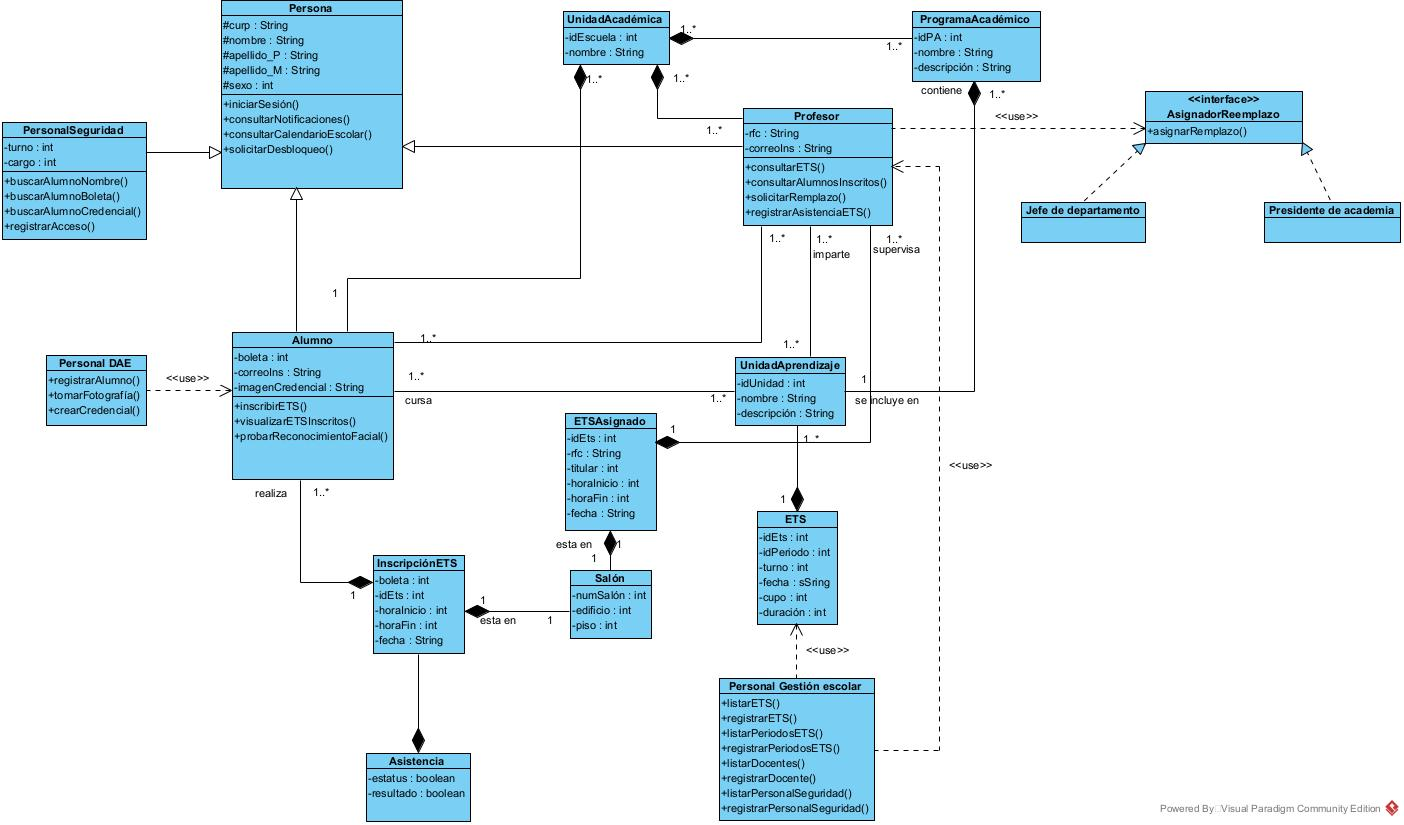
\includegraphics[width=.35\textwidth]{Clases/Clases}}
		\caption{Diagrama de clases.}
		\label{fig:Diagrama de clases}
	\end{center}
\end{figure}

\section{Diagramas de secuencia}

\begin{figure}[htbp!]
	\begin{center}
		\fbox{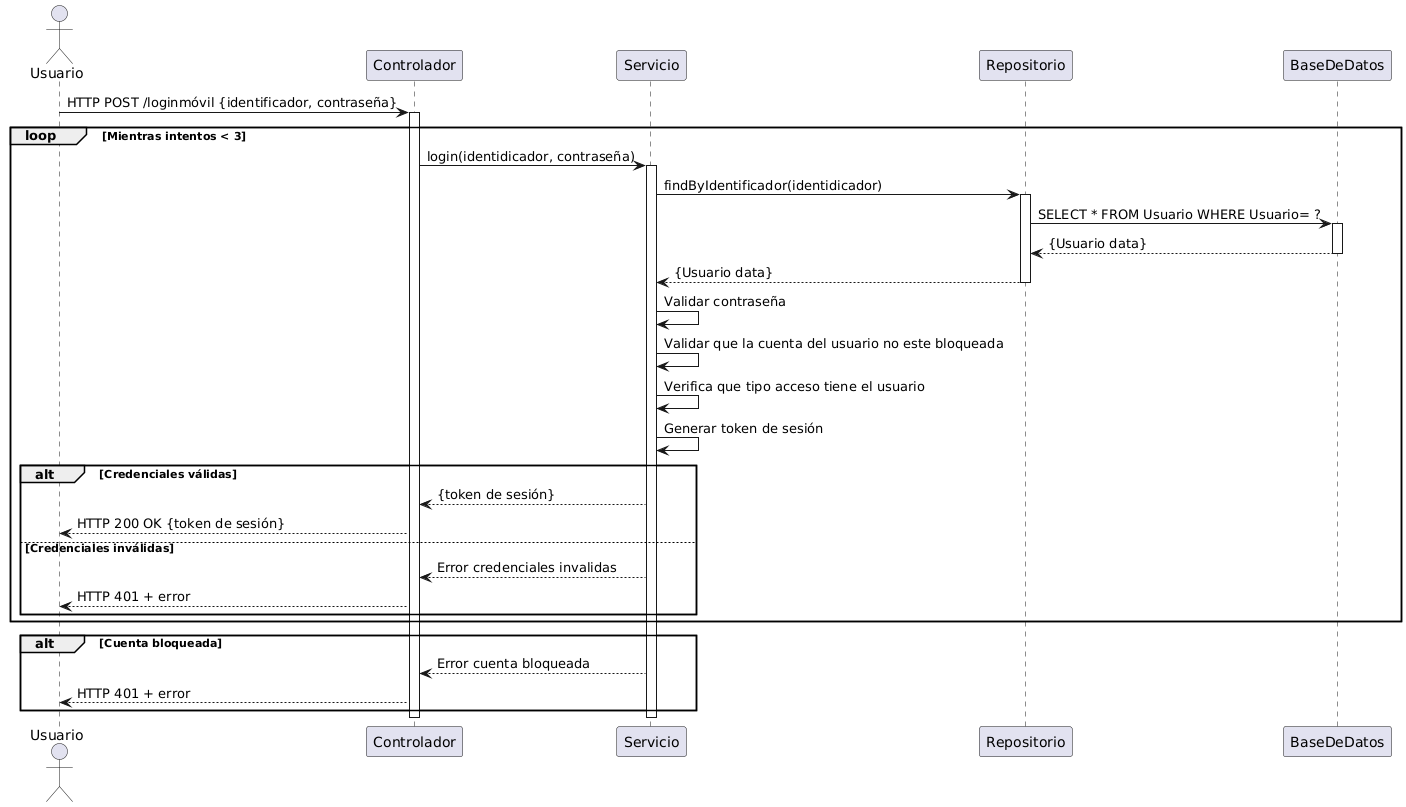
\includegraphics[width=.35\textwidth]{Secuencia/CU-01.png}}
		\caption{Diagrama de secuencia del caso de uso número 01 (Iniciar sesión del sistema móvil).}
		\label{fig:Diagrama de secuencia CU-01}
	\end{center}
\end{figure}

\begin{figure}[htbp!]
	\begin{center}
		\fbox{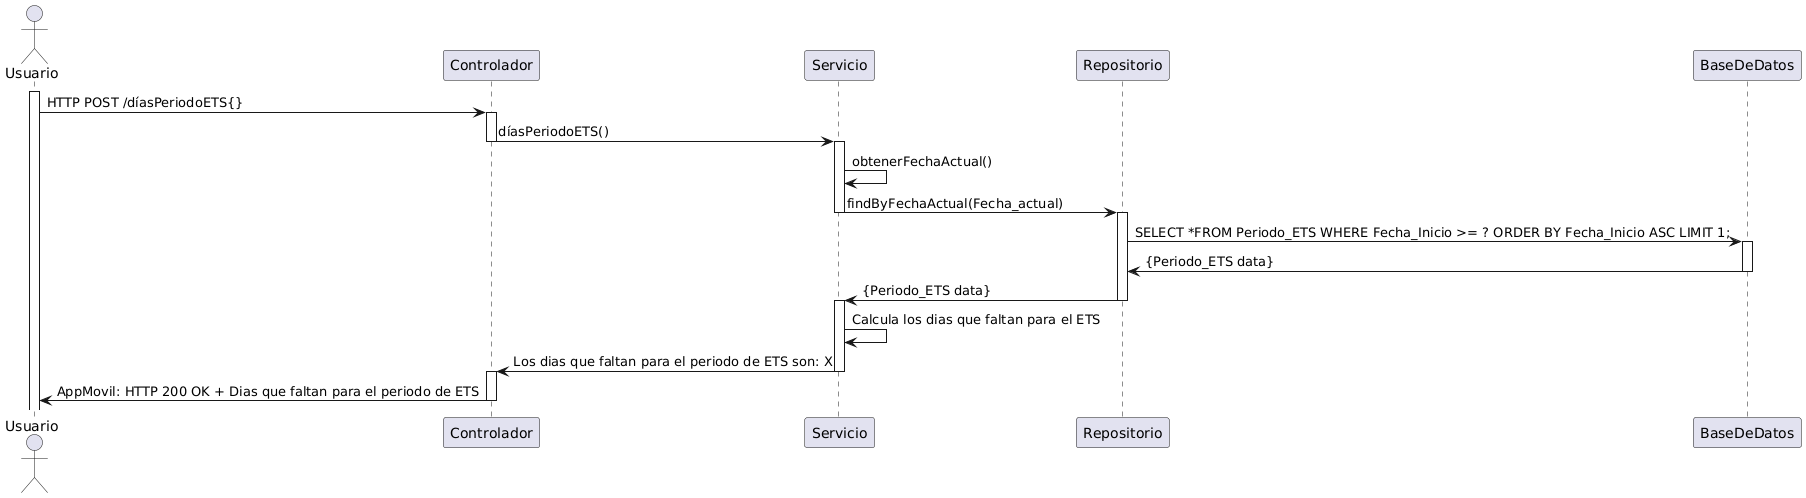
\includegraphics[width=.35\textwidth]{Secuencia/CU-02.png}}
		\caption{Diagrama de secuencia del caso de uso número 02 (Consultar calendario escolar).}
		\label{fig:Diagrama de secuencia CU-02}
	\end{center}
\end{figure}

\begin{figure}[htbp!]
	\begin{center}
		\fbox{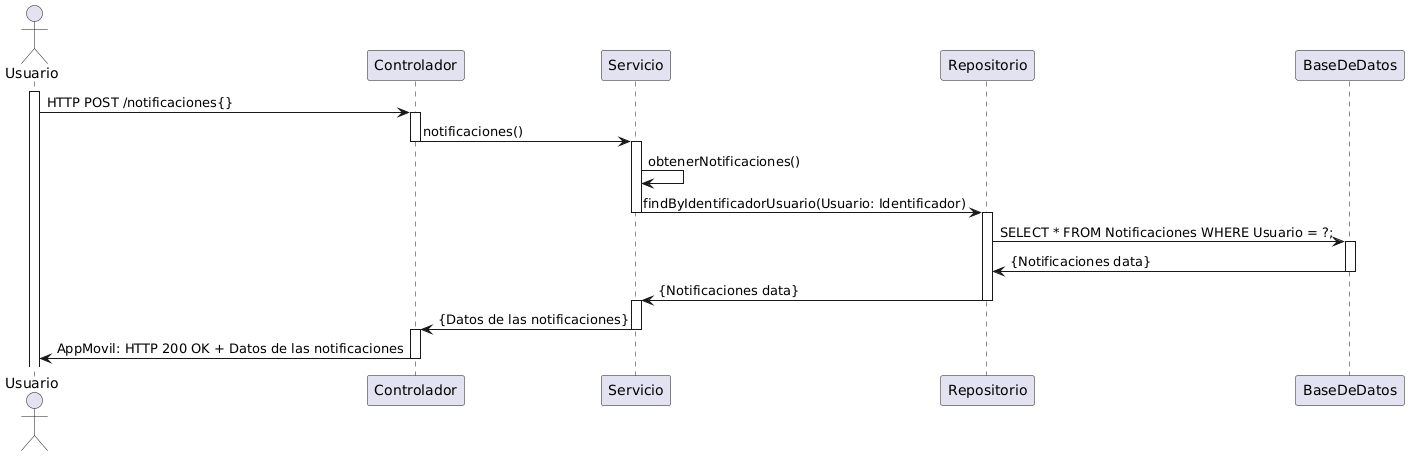
\includegraphics[width=.35\textwidth]{Secuencia/CU-03.png}}
		\caption{Diagrama de secuencia del caso de uso número 03 (Consultar notificaciones).}
		\label{fig:Diagrama se secuencia CU-03}
	\end{center}
\end{figure}

\begin{figure}[htbp!]
	\begin{center}
		\fbox{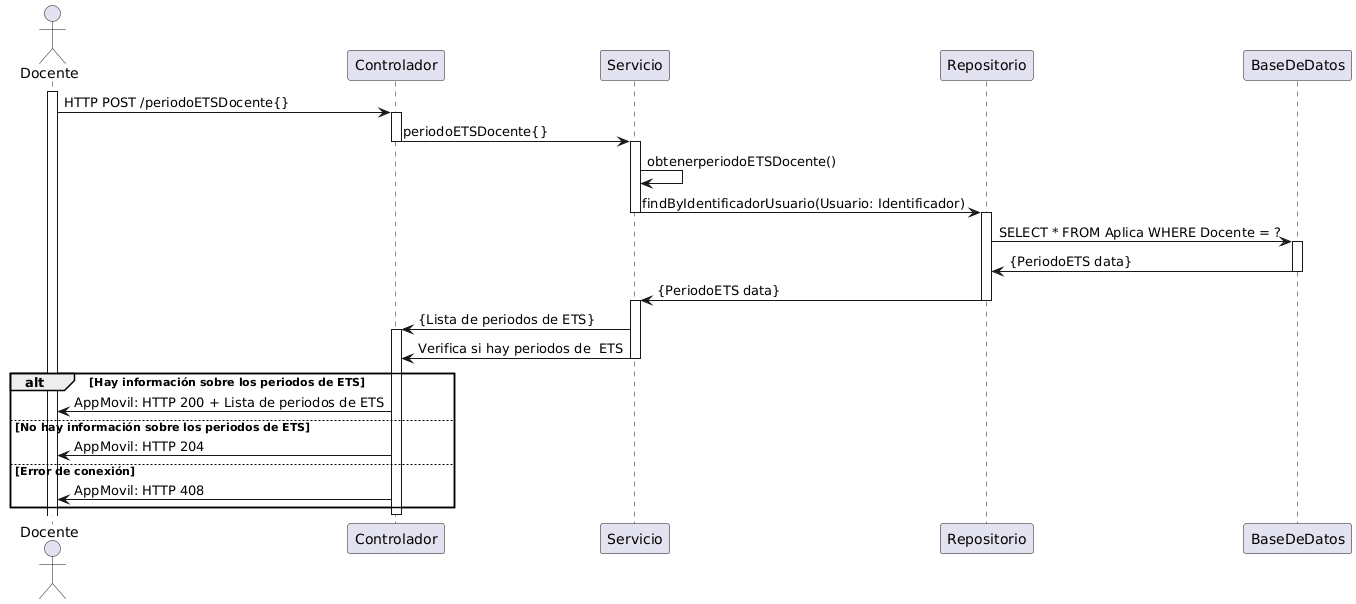
\includegraphics[width=.35\textwidth]{Secuencia/CU-04.png}}
		\caption{Diagrama de secuencia del caso de uso número 04 (Consultar periodos de ETS asignados al docente).}
		\label{fig:Diagrama de secuencia CU-04}
	\end{center}
\end{figure}

\begin{figure}[htbp!]
	\begin{center}
		\fbox{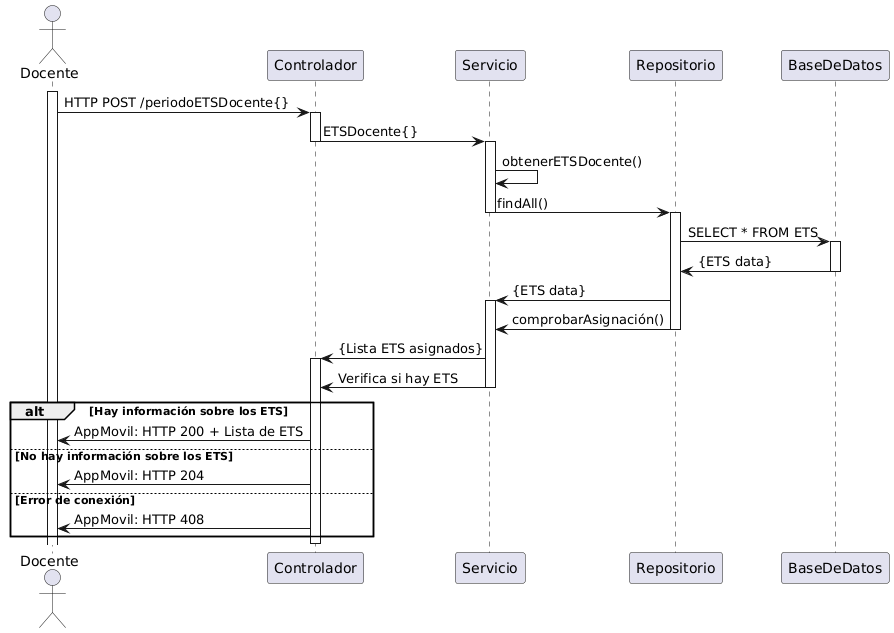
\includegraphics[width=.35\textwidth]{Secuencia/CU-05.png}}
		\caption{Diagrama de secuencia del caso de uso número 05 (Consultar ETS asignados).}
		\label{fig:Diagrama de secuencia CU-05}
	\end{center}
\end{figure}

\begin{figure}[htbp!]
	\begin{center}
		\fbox{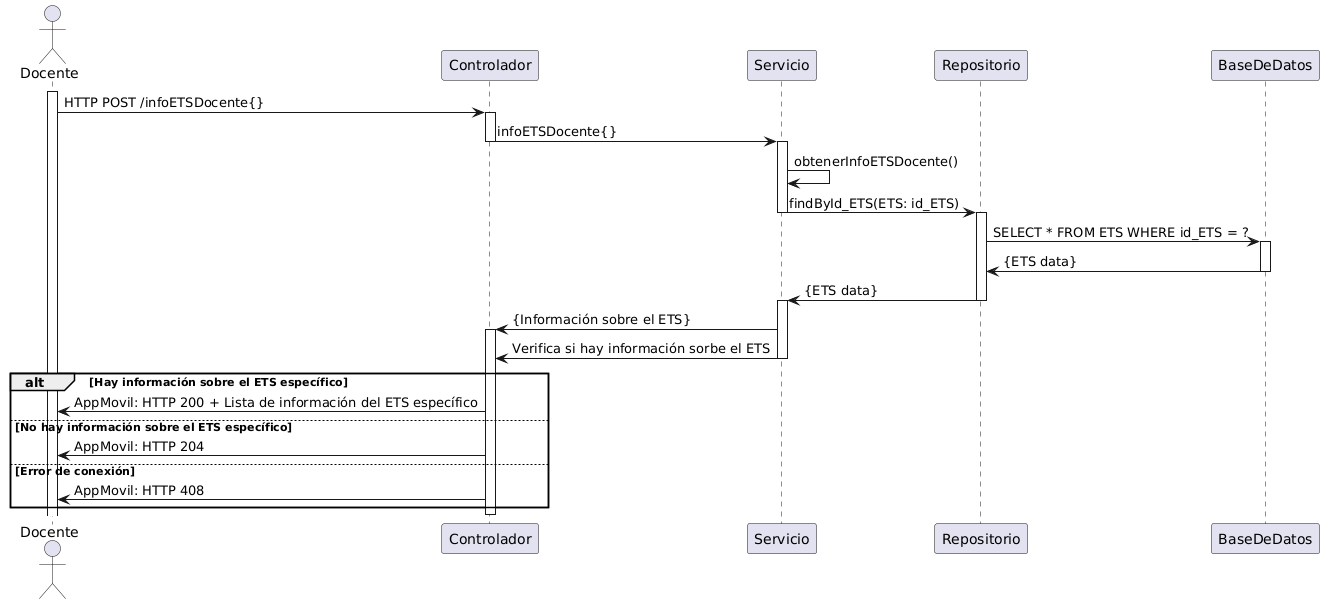
\includegraphics[width=.35\textwidth]{Secuencia/CU-06.png}}
		\caption{Diagrama de secuencia del caso de uso número 06 (CU-06).}
		\label{fig:Diagrama de secuencia CU-06}
	\end{center}
\end{figure}

\begin{figure}[htbp!]
	\begin{center}
		\fbox{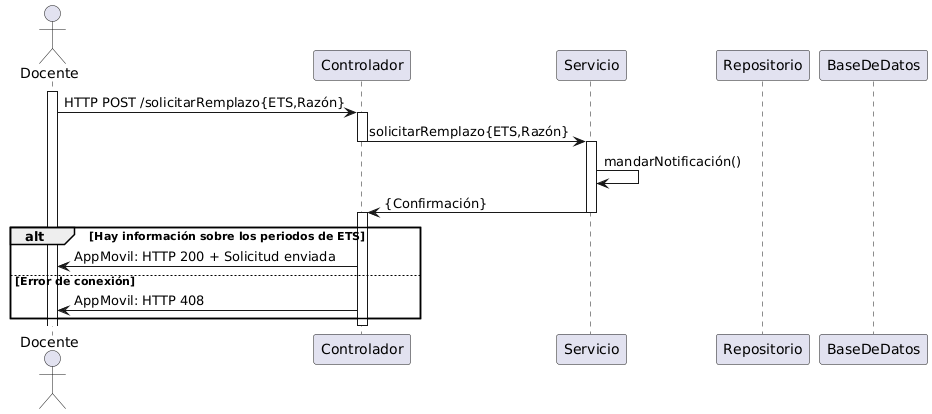
\includegraphics[width=.35\textwidth]{Secuencia/CU-07.png}}
		\caption{Diagrama de secuencia del caso de uso número 07 (CU-07).}
		\label{fig:Diagrama de secuencia CU-07}
	\end{center}
\end{figure}

\begin{figure}[htbp!]
	\begin{center}
		\fbox{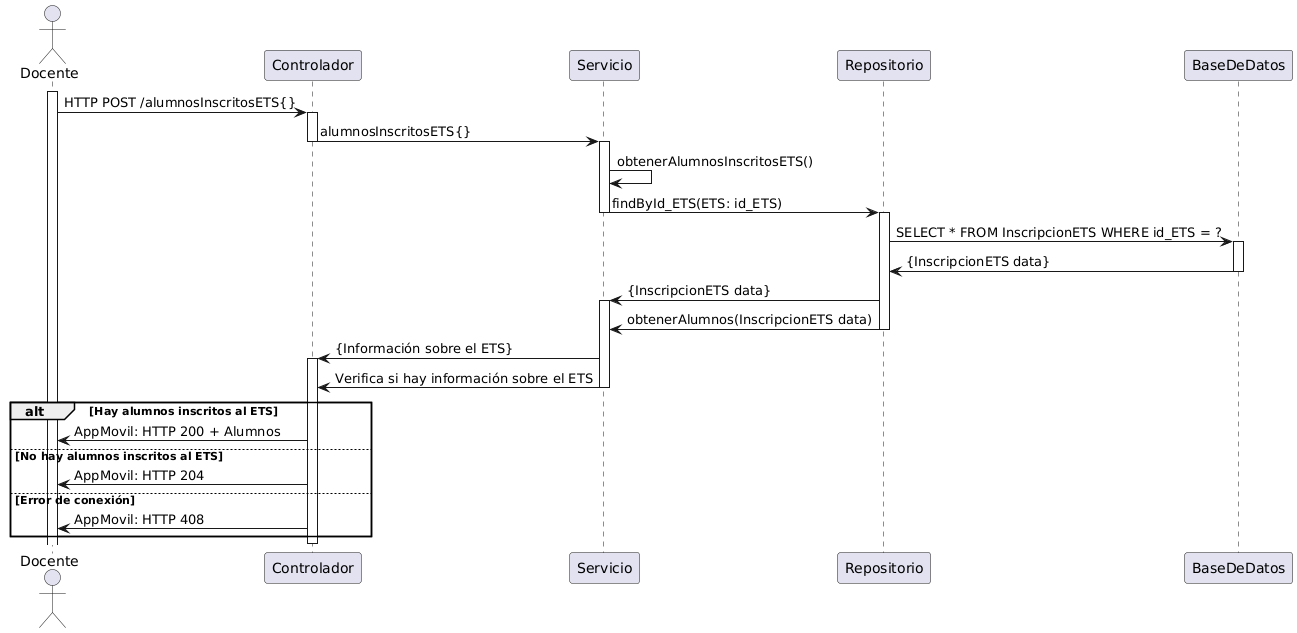
\includegraphics[width=.35\textwidth]{Secuencia/CU-08.png}}
		\caption{Diagrama de secuencia del caso de uso número 08 (CU-08).}
		\label{fig:Diagrama de secuencia CU-08}
	\end{center}
\end{figure}

\begin{figure}[htbp!]
	\begin{center}
		\fbox{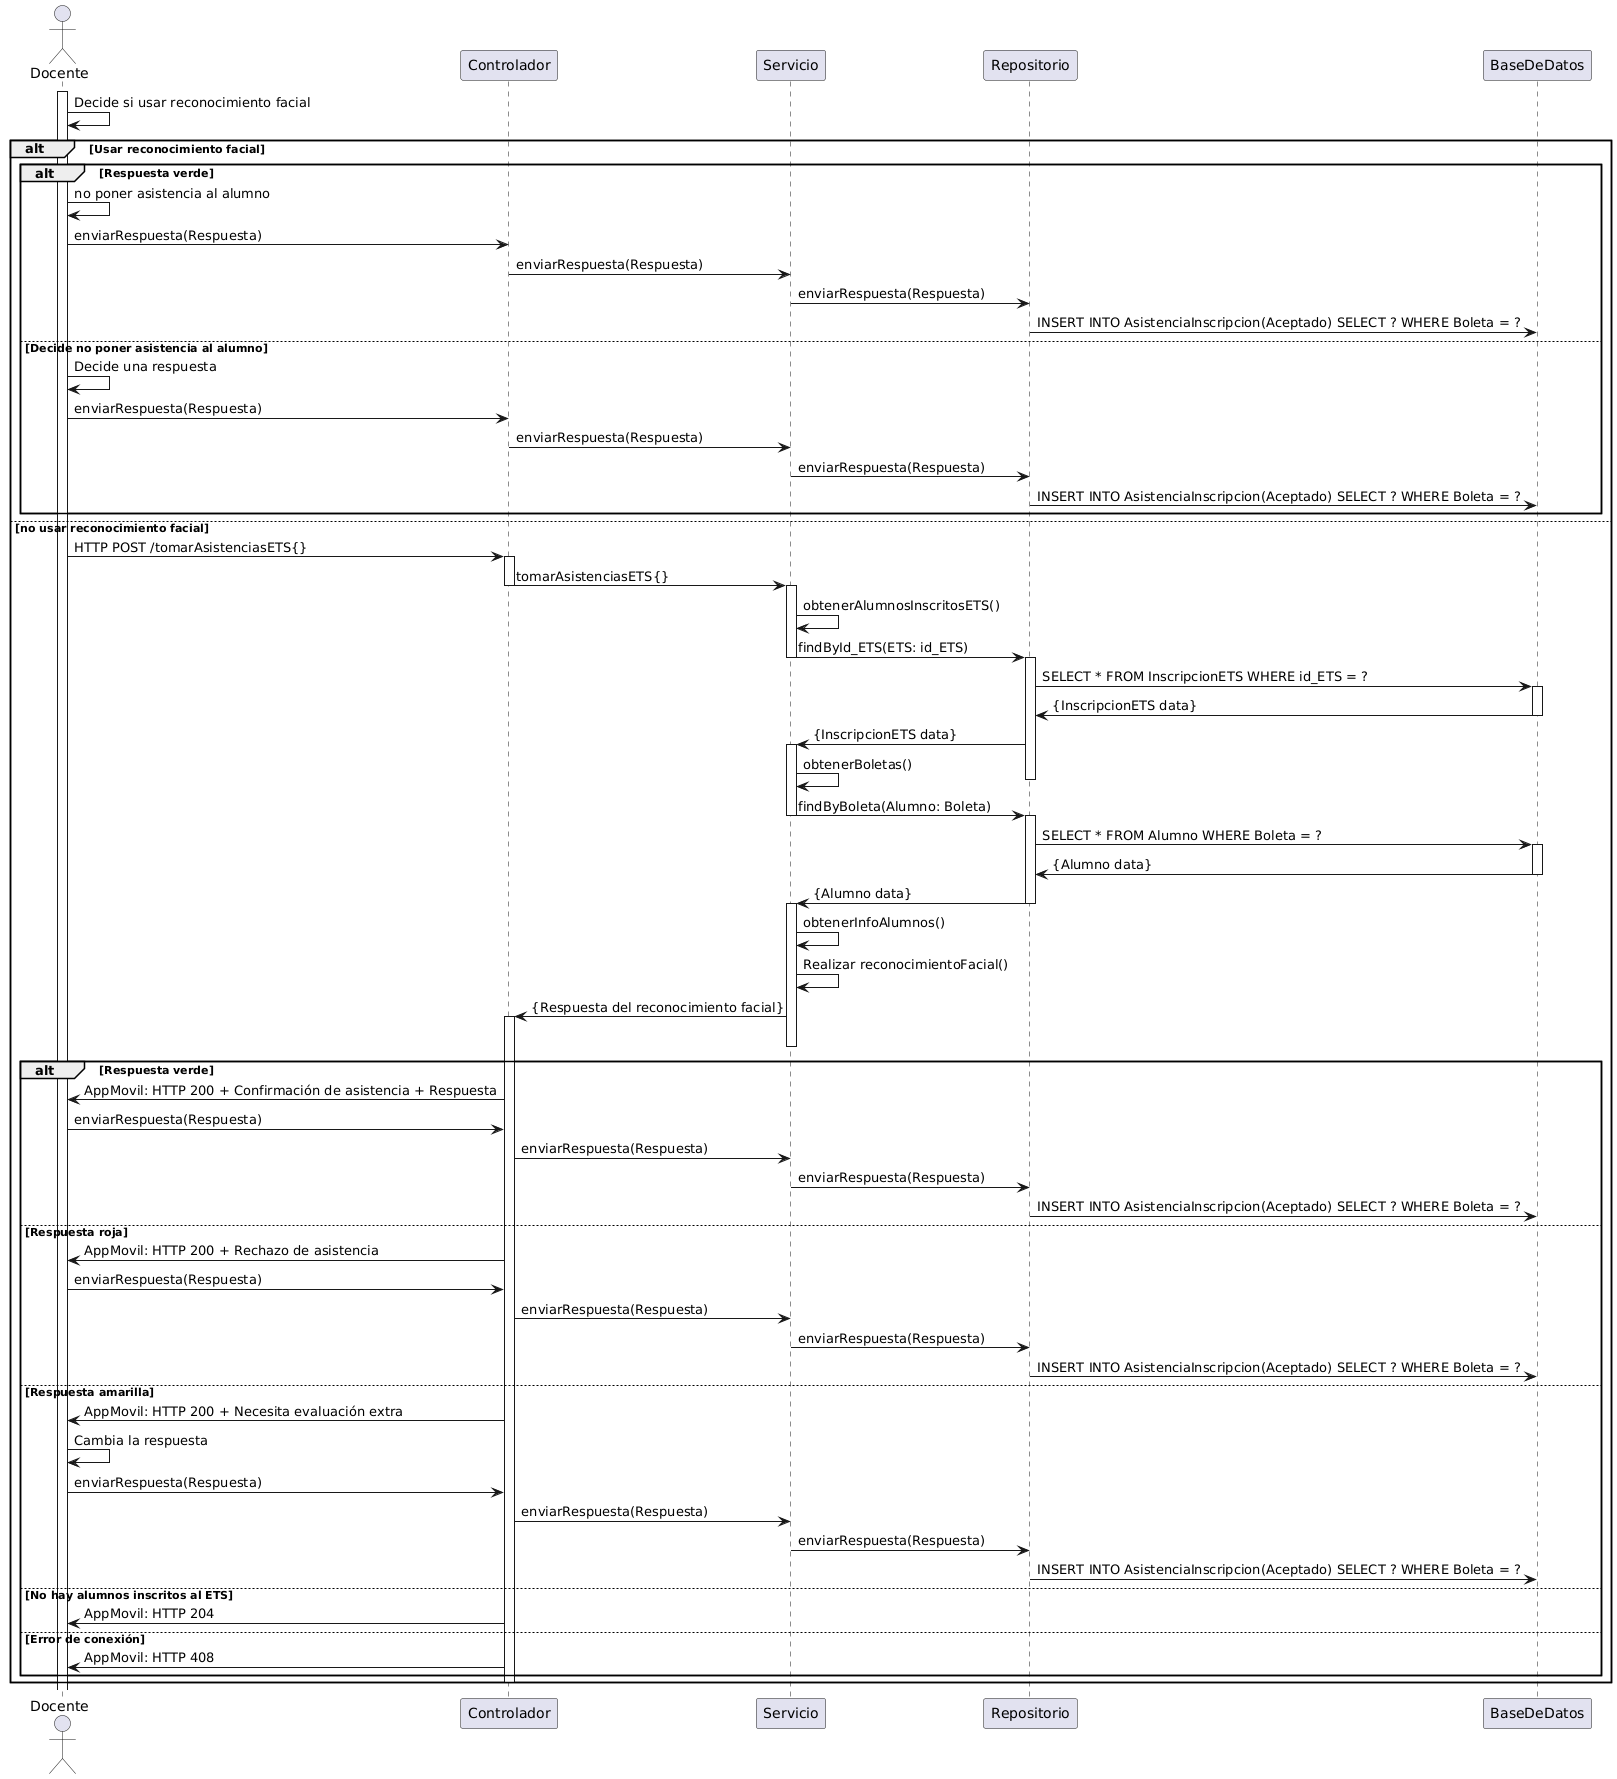
\includegraphics[width=.35\textwidth]{Secuencia/CU-09.png}}
		\caption{Diagrama de secuencia del caso de uso número 09 (CU-09).}
		\label{fig:Diagrama de secuencia CU-09}
	\end{center}
\end{figure}

\begin{figure}[htbp!]
	\begin{center}
		\fbox{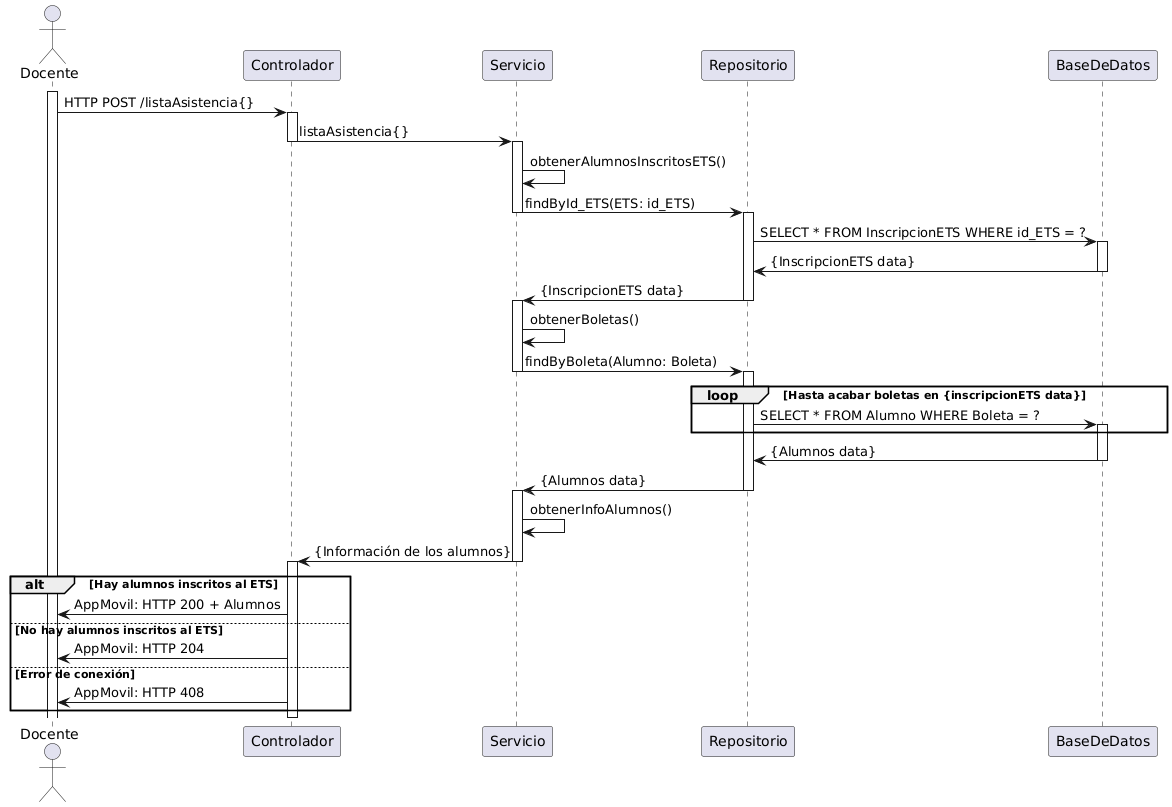
\includegraphics[width=.35\textwidth]{Secuencia/CU-10.png}}
		\caption{Diagrama de secuencia del caso de uso número 10 (CU-10).}
		\label{fig:Diagrama de secuencia CU-10}
	\end{center}
\end{figure}

\begin{figure}[htbp!]
	\begin{center}
		\fbox{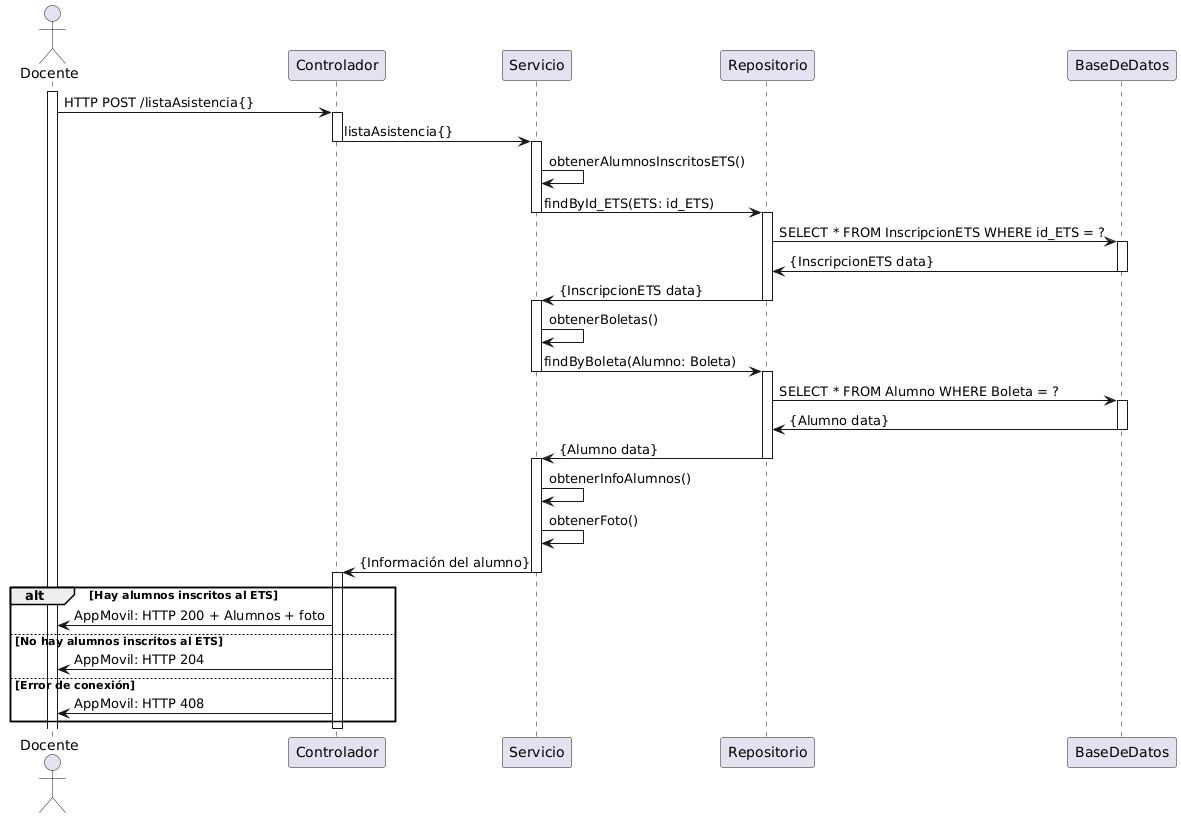
\includegraphics[width=.35\textwidth]{Secuencia/CU-11.png}}
		\caption{Diagrama de secuencia del caso de uso número 11 (CU-11).}
		\label{fig:Diagrama de secuencia CU-1}
	\end{center}
\end{figure}

\begin{figure}[htbp!]
	\begin{center}
		\fbox{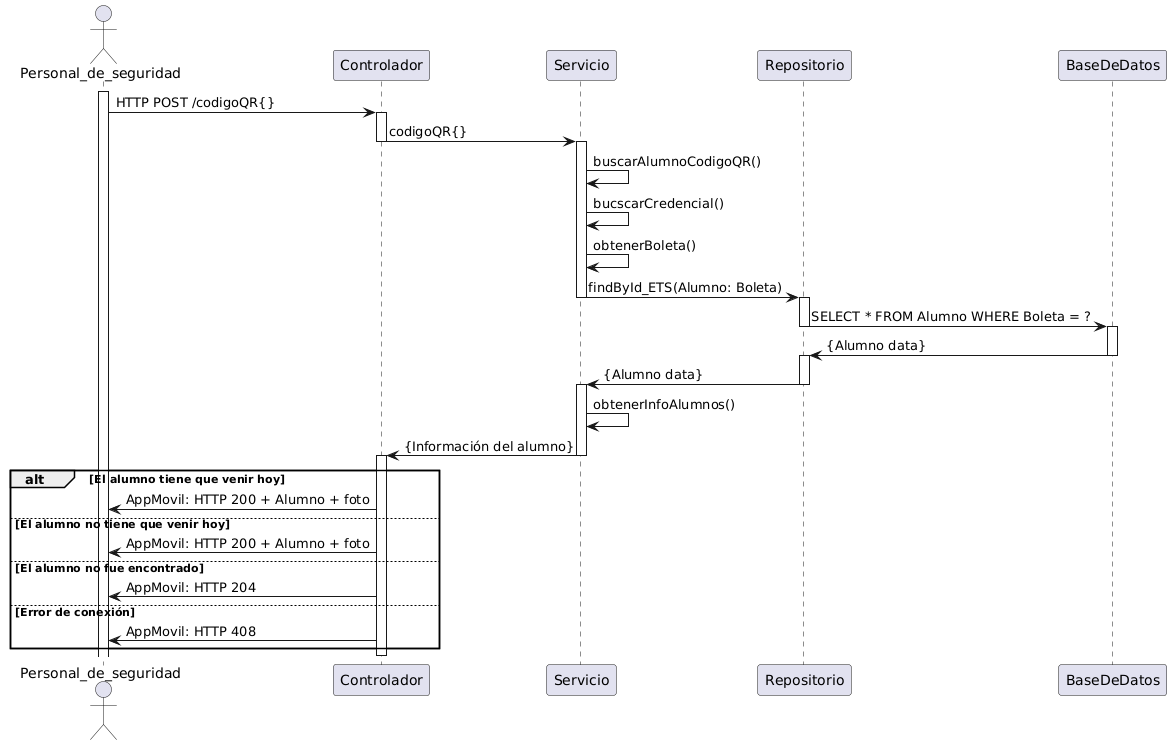
\includegraphics[width=.35\textwidth]{Secuencia/CU-12.png}}
		\caption{Diagrama de secuencia del caso de uso número 12 (CU-12).}
		\label{fig:Diagrama de secuencia CU-12}
	\end{center}
\end{figure}

\begin{figure}[htbp!]
	\begin{center}
		\fbox{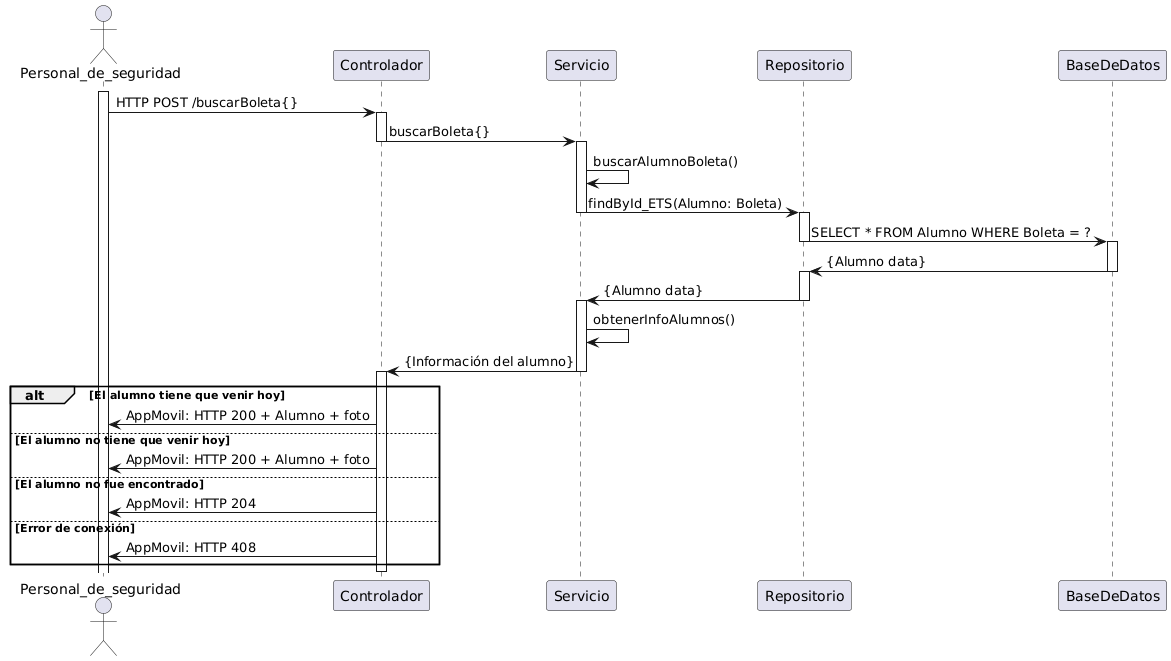
\includegraphics[width=.35\textwidth]{Secuencia/CU-13.png}}
		\caption{Diagrama de secuencia del caso de uso número 13 (CU-13).}
		\label{fig:Diagrama de secuencia CU-13}
	\end{center}
\end{figure}

\begin{figure}[htbp!]
	\begin{center}
		\fbox{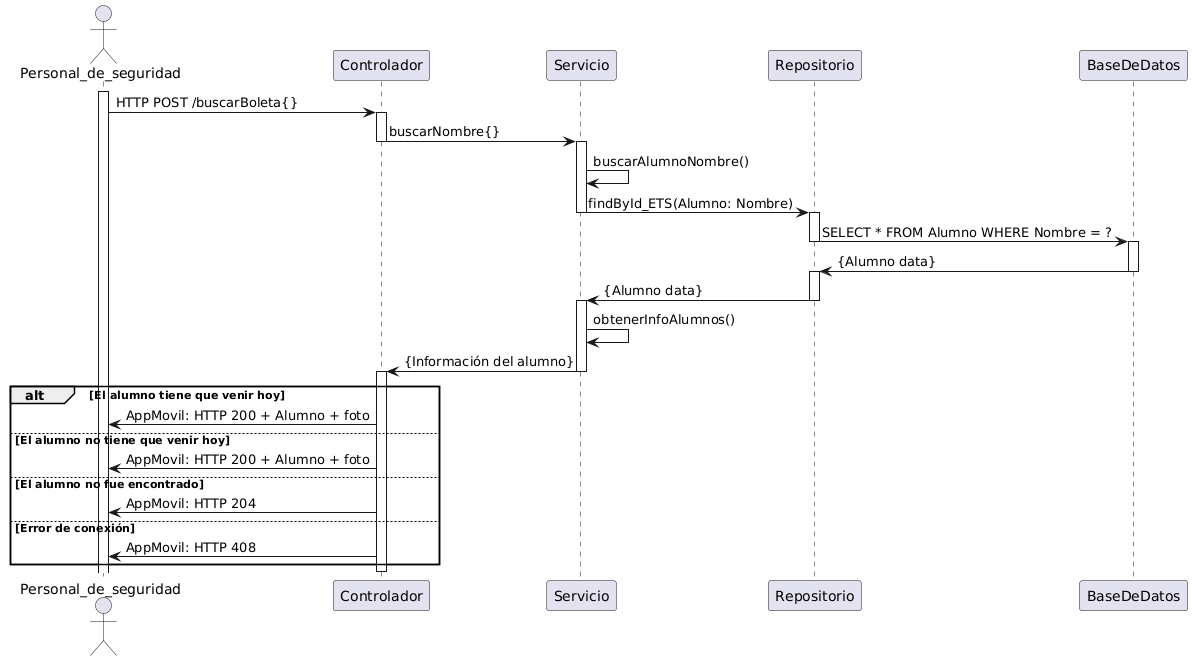
\includegraphics[width=.35\textwidth]{Secuencia/CU-14.png}}
		\caption{Diagrama de secuencia del caso de uso número 14 (CU-14).}
		\label{fig:Diagrama de secuencia CU-14}
	\end{center}
\end{figure}

\begin{figure}[htbp!]
	\begin{center}
		\fbox{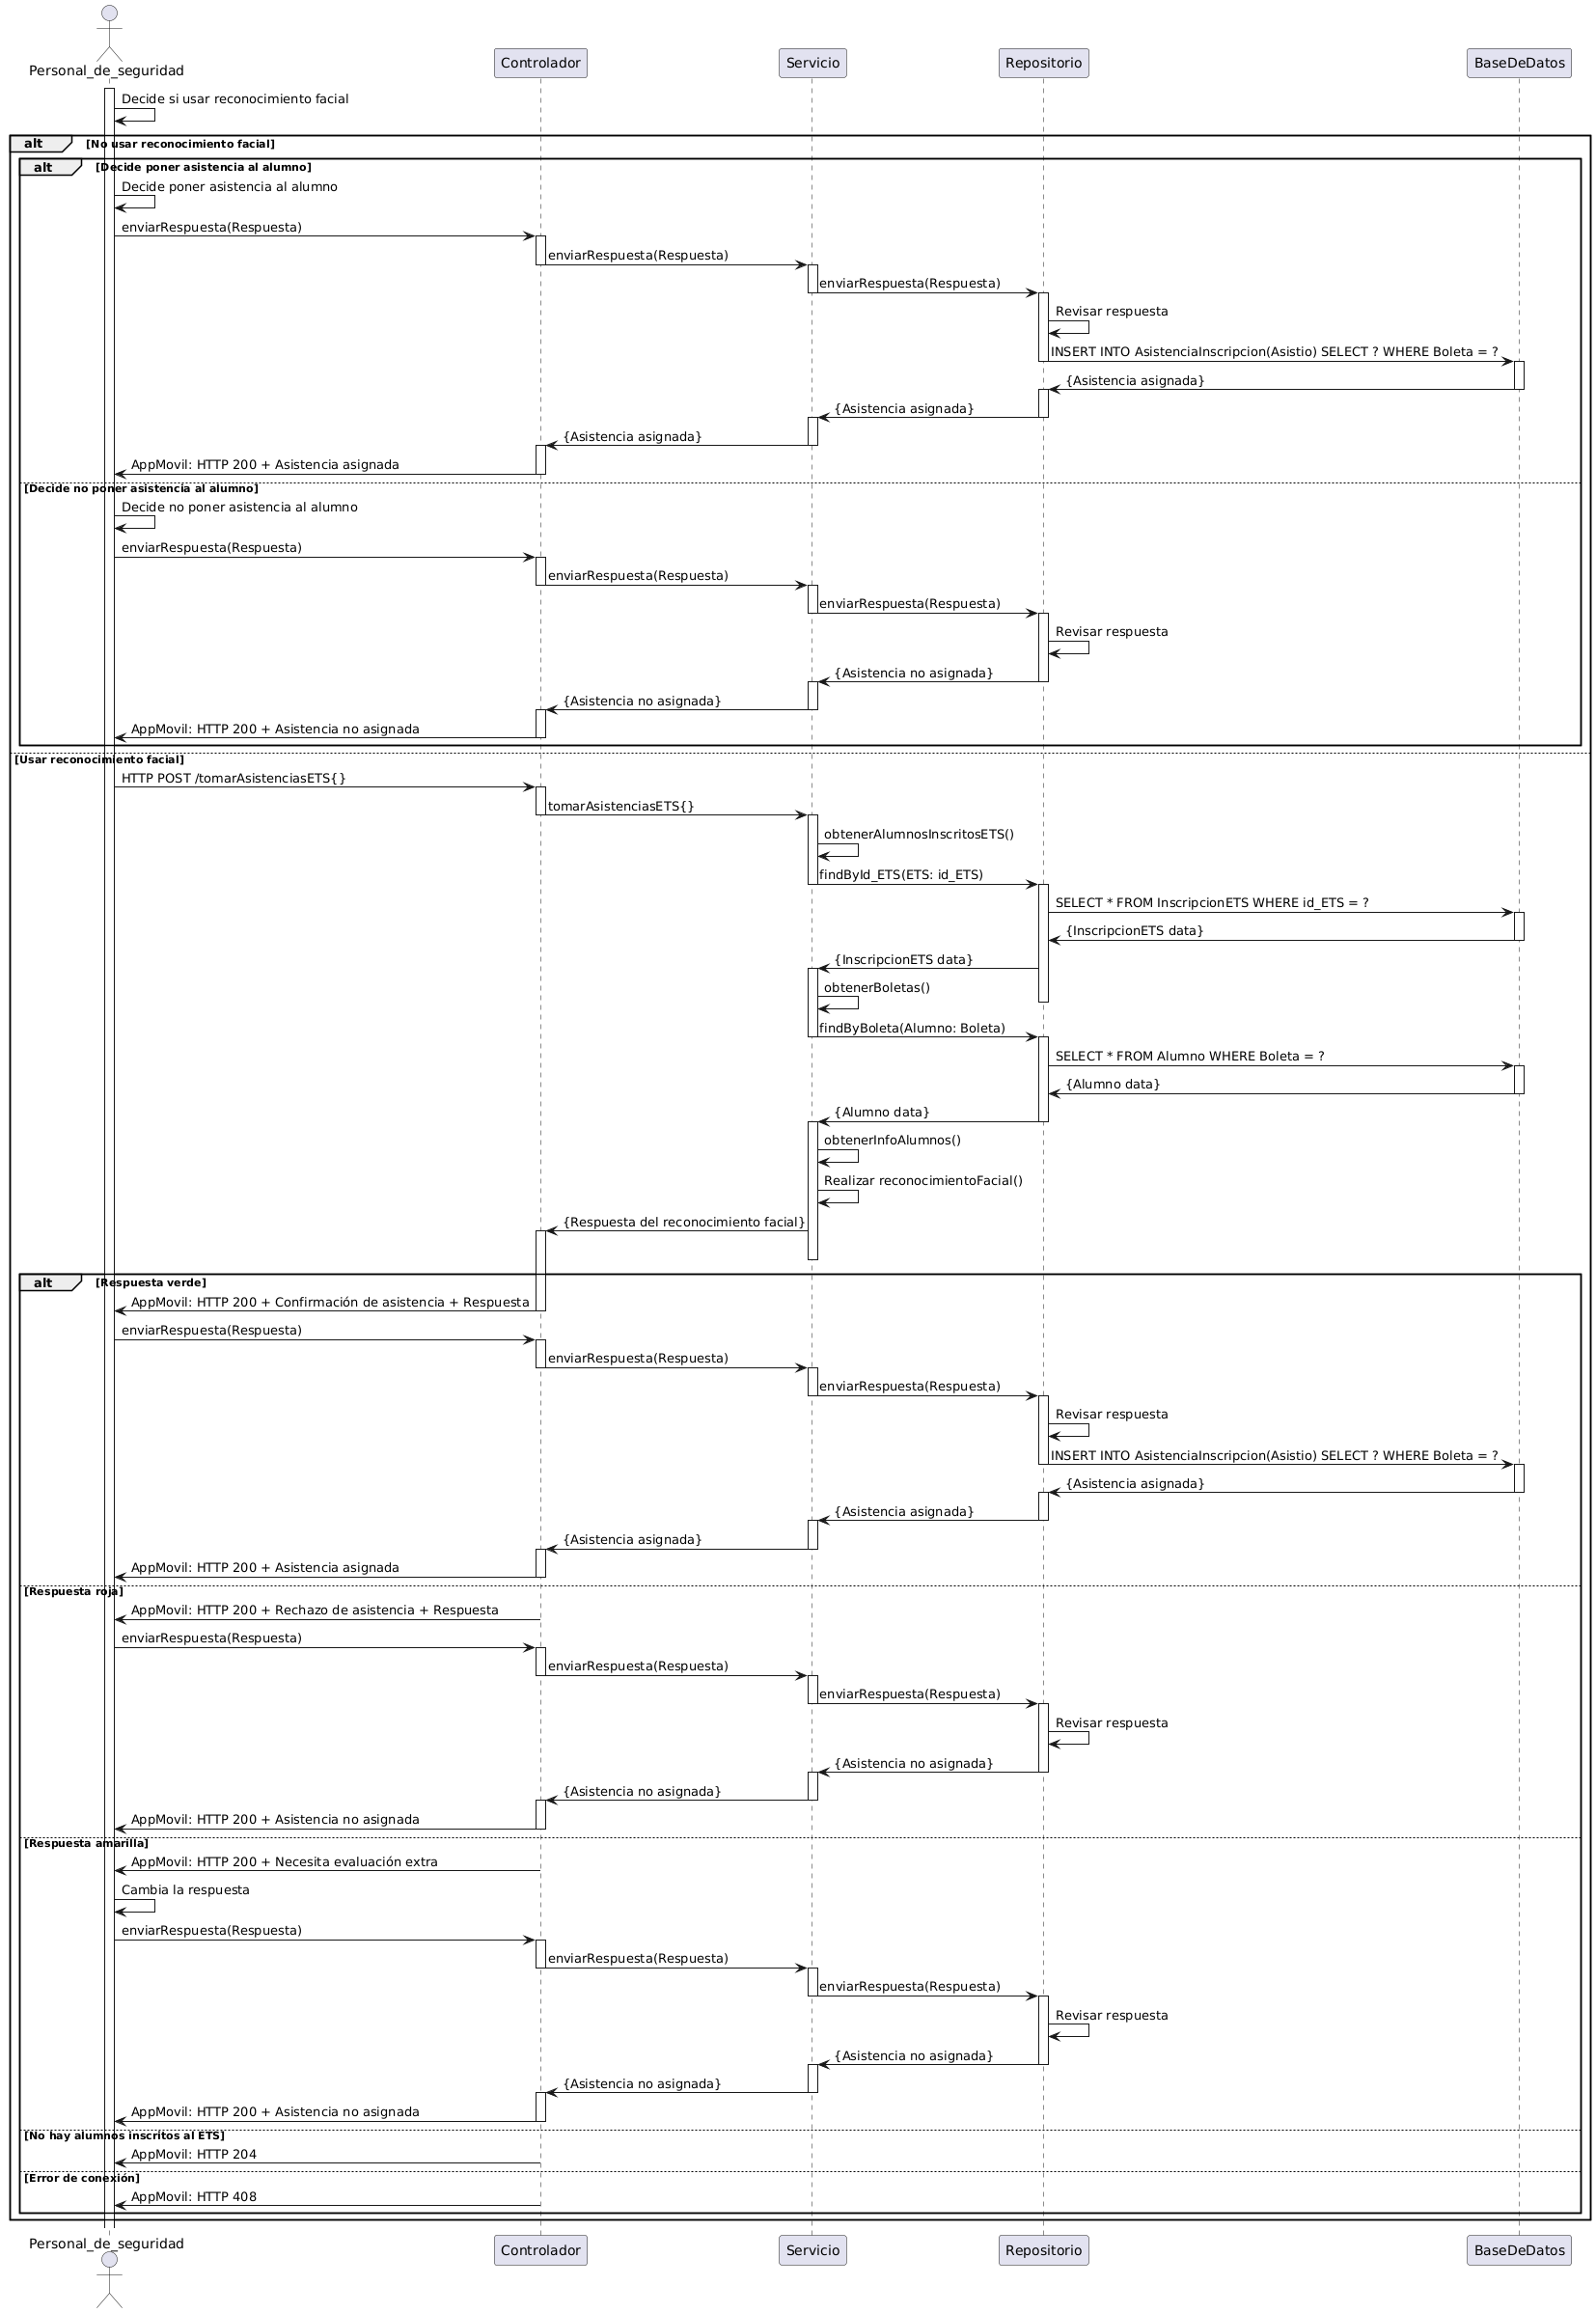
\includegraphics[width=.35\textwidth]{Secuencia/CU-15.png}}
		\caption{Diagrama de secuencia del caso de uso número 15 (CU-15).}
		\label{fig:Diagrama de secuencia CU-15}
	\end{center}
\end{figure}

\begin{figure}[htbp!]
	\begin{center}
		\fbox{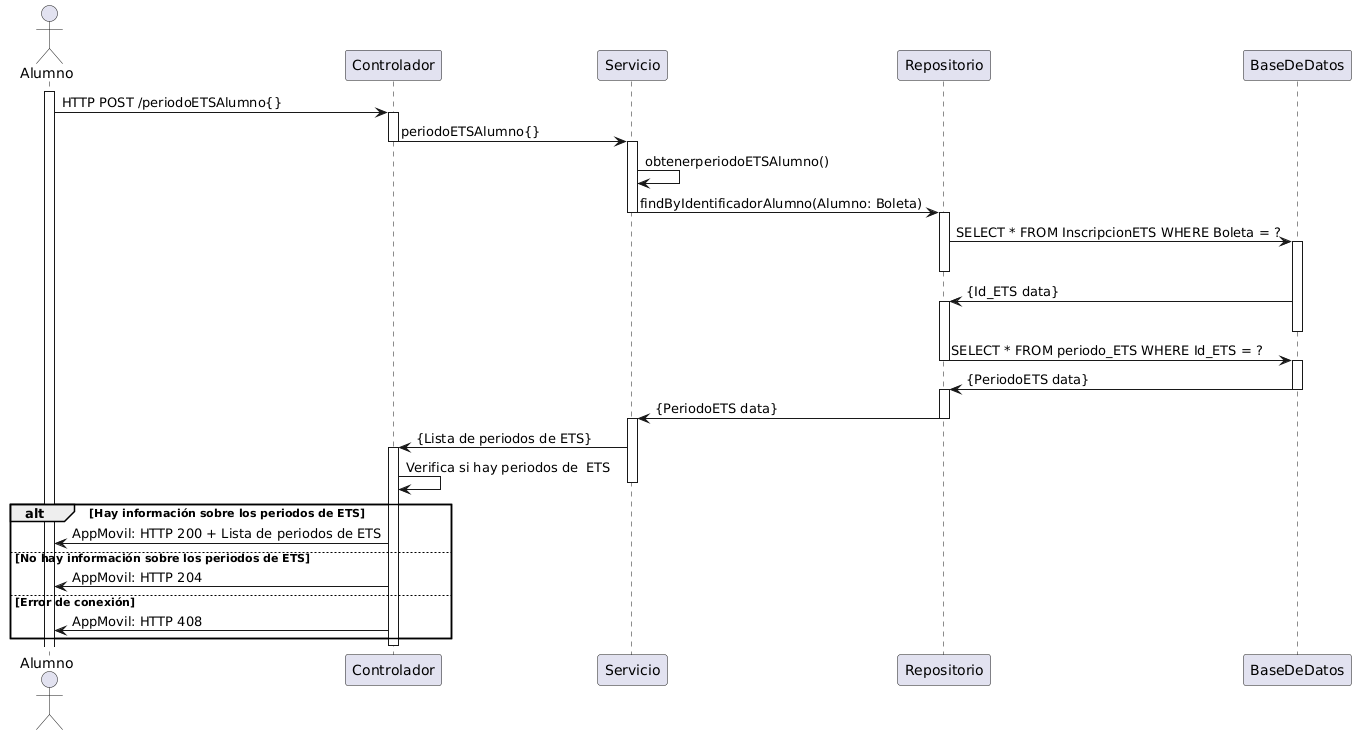
\includegraphics[width=.35\textwidth]{Secuencia/CU-16.png}}
		\caption{Diagrama de secuencia del caso de uso número 16 (CU-16).}
		\label{fig:Diagrama de secuencia CU-16}
	\end{center}
\end{figure}

\begin{figure}[htbp!]
	\begin{center}
		\fbox{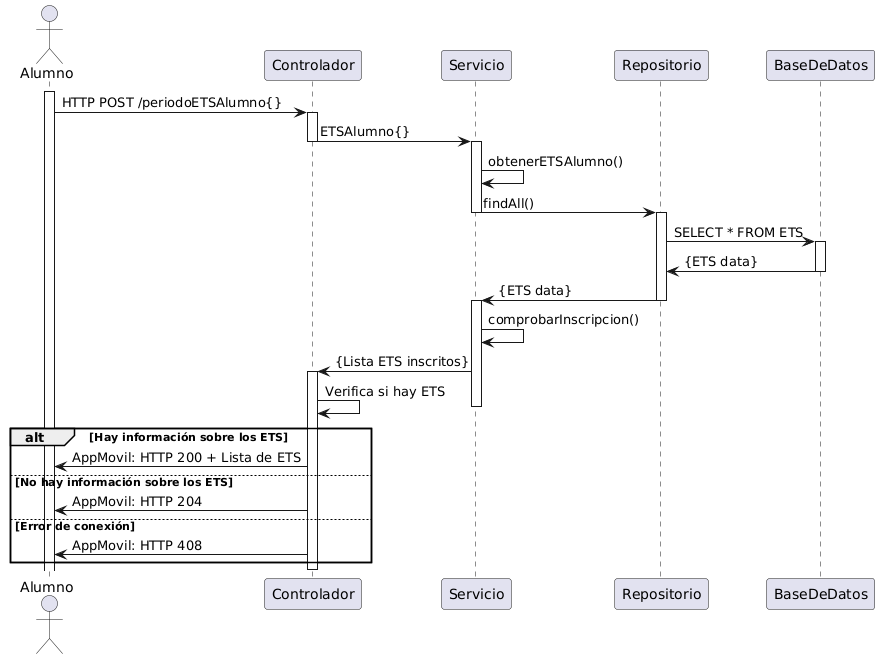
\includegraphics[width=.35\textwidth]{Secuencia/CU-17.png}}
		\caption{Diagrama de secuencia del caso de uso número 04 (CU-17).}
		\label{fig:Diagrama de secuencia CU-17}
	\end{center}
\end{figure}

\begin{figure}[htbp!]
	\begin{center}
		\fbox{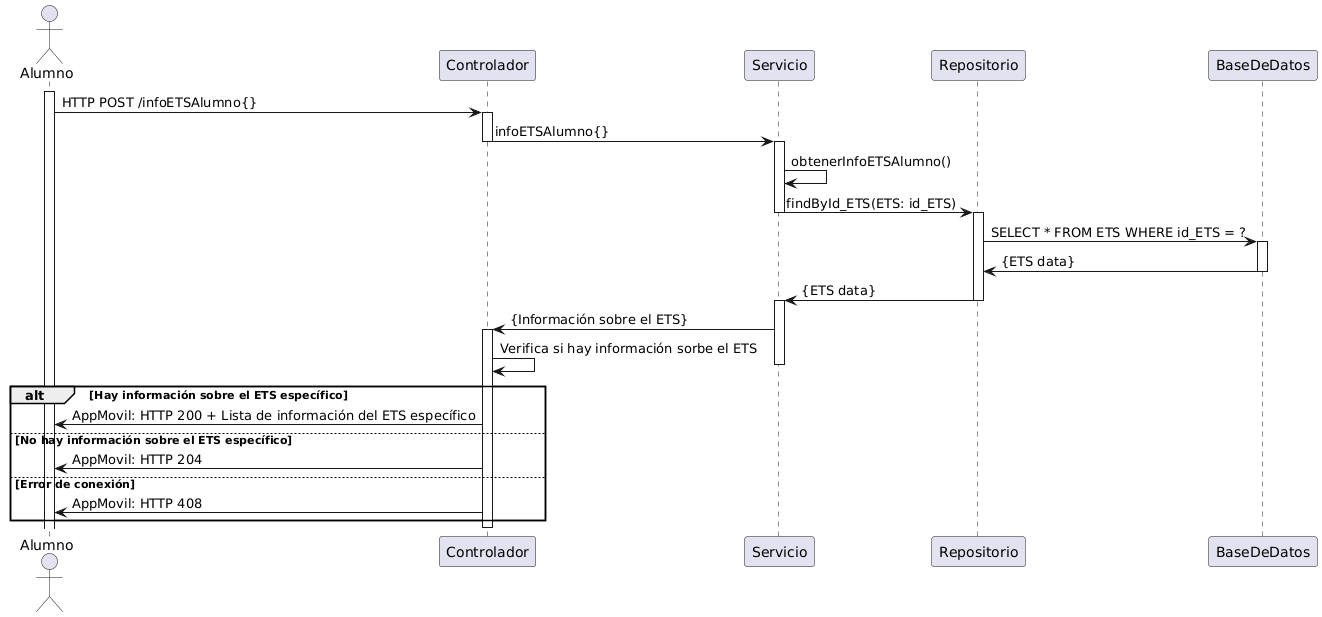
\includegraphics[width=.35\textwidth]{Secuencia/CU-18.png}}
		\caption{Diagrama de secuencia del caso de uso número 18 (CU-18).}
		\label{fig:Diagrama de secuencia CU-18}
	\end{center}
\end{figure}

\begin{figure}[htbp!]
	\begin{center}
		\fbox{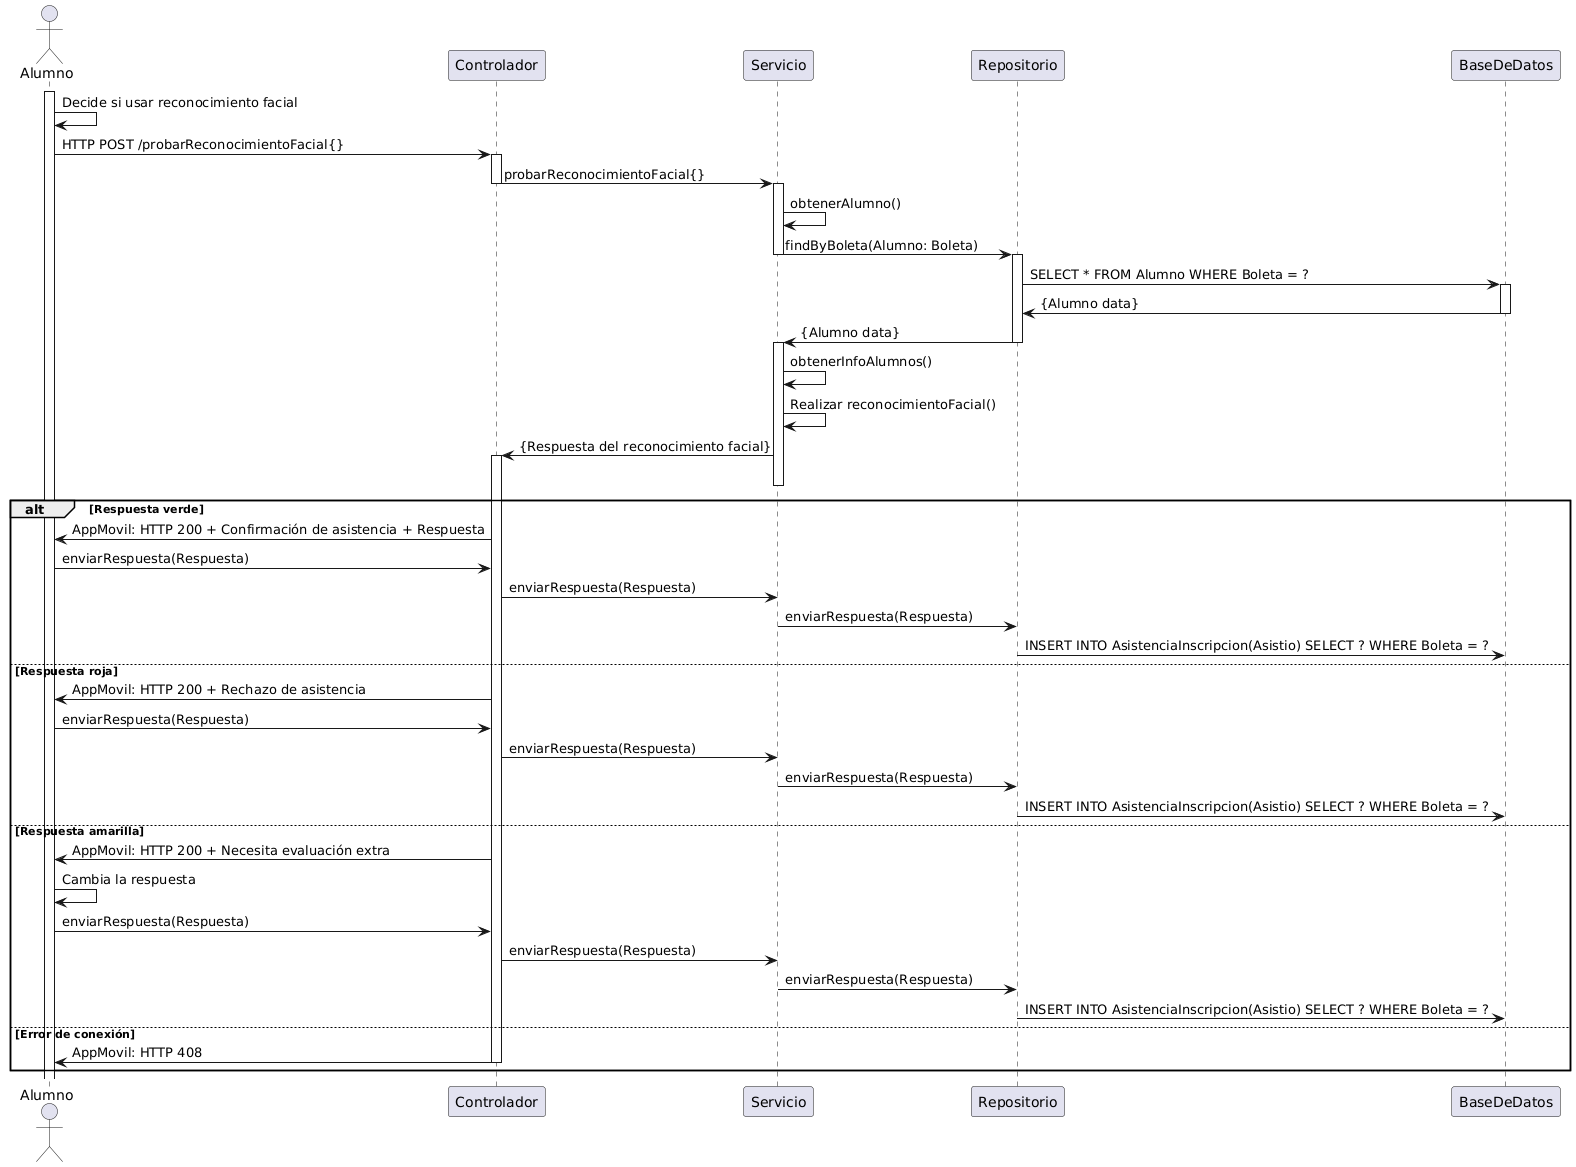
\includegraphics[width=.35\textwidth]{Secuencia/CU-19.png}}
		\caption{Diagrama de secuencia del caso de uso número 19 (CU-19).}
		\label{fig:Diagrama de secuencia CU-19}
	\end{center}
\end{figure}

\begin{figure}[htbp!]
	\begin{center}
		\fbox{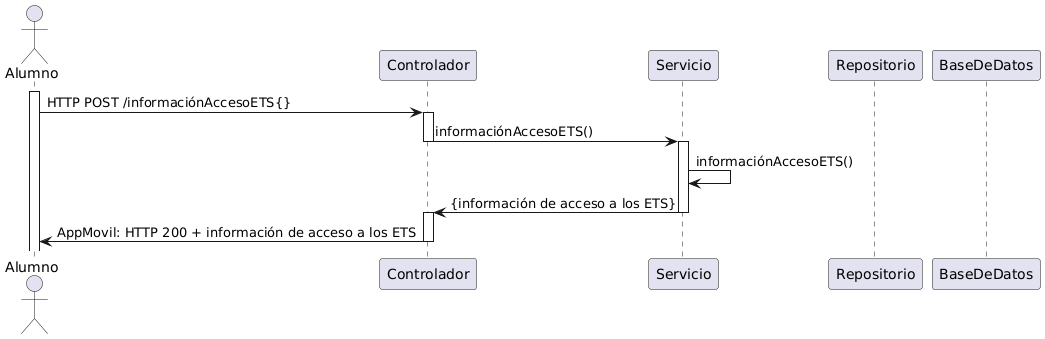
\includegraphics[width=.35\textwidth]{Secuencia/CU-20.png}}
		\caption{Diagrama de secuencia del caso de uso número 20 (CU-20).}
		\label{fig:Diagrama de secuencia CU-20}
	\end{center}
\end{figure}

\begin{figure}[htbp!]
	\begin{center}
		\fbox{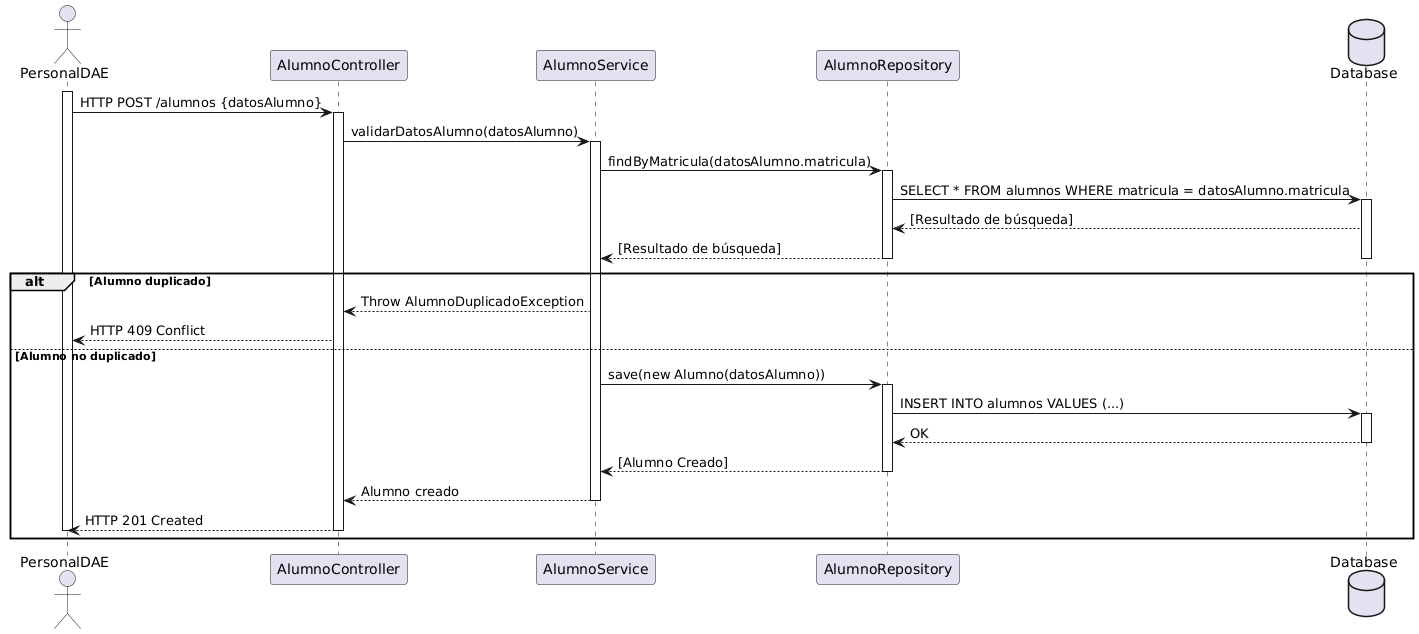
\includegraphics[width=.35\textwidth]{Secuencia/CU-21.png}}
		\caption{Diagrama de secuencia del caso de uso número 21 (CU-21).}
		\label{fig:Diagrama de secuencia CU-21}
	\end{center}
\end{figure}

\begin{figure}[htbp!]
	\begin{center}
		\fbox{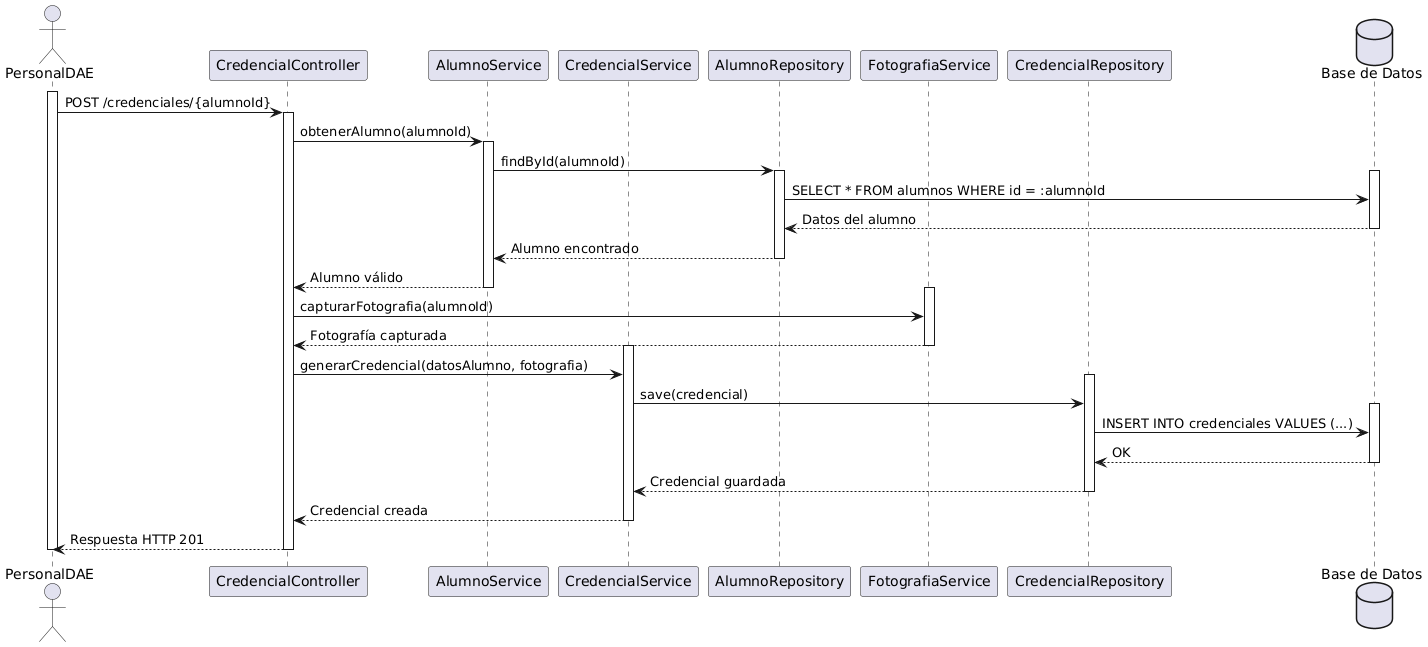
\includegraphics[width=.35\textwidth]{Secuencia/CU-22_23.png}}
		\caption{Diagrama de secuencia del caso de uso número 22 y 23 (CU-22 y CU23).}
		\label{fig:Diagrama de secuencia CU-22 y CU23}
	\end{center}
\end{figure}

\begin{figure}[htbp!]
	\begin{center}
		\fbox{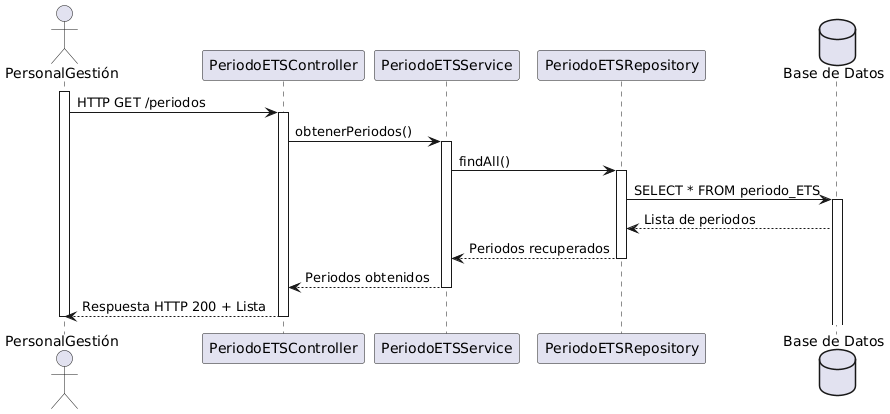
\includegraphics[width=.35\textwidth]{Secuencia/CU-24.png}}
		\caption{Diagrama de secuencia del caso de uso número 24 (CU-24).}
		\label{fig:Diagrama de secuencia CU-24}
	\end{center}
\end{figure}

\begin{figure}[htbp!]
	\begin{center}
		\fbox{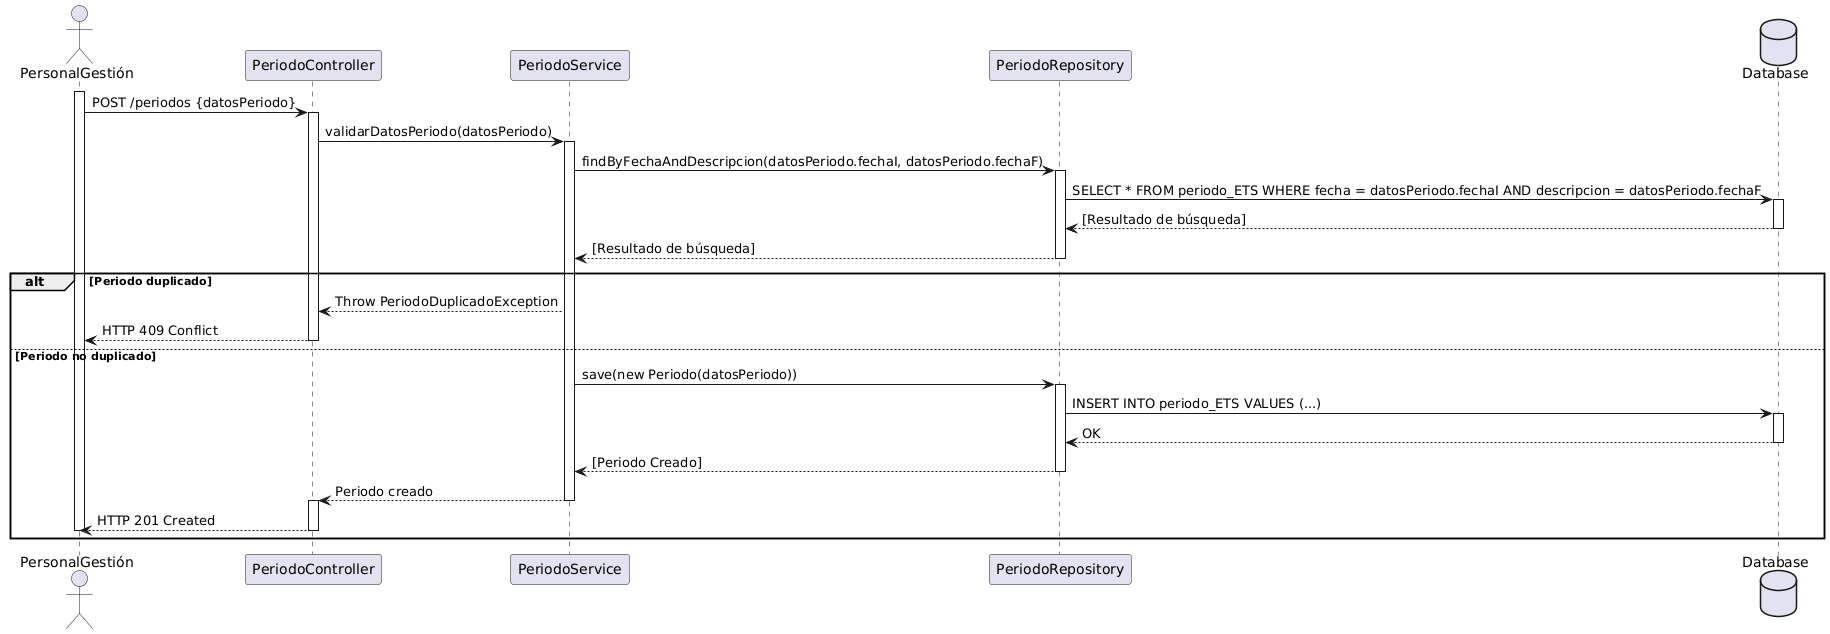
\includegraphics[width=.35\textwidth]{Secuencia/CU-25.png}}
		\caption{Diagrama de secuencia del caso de uso número 25 (CU-25).}
		\label{fig:Diagrama de secuencia CU-24}
	\end{center}
\end{figure}

\begin{figure}[htbp!]
	\begin{center}
		\fbox{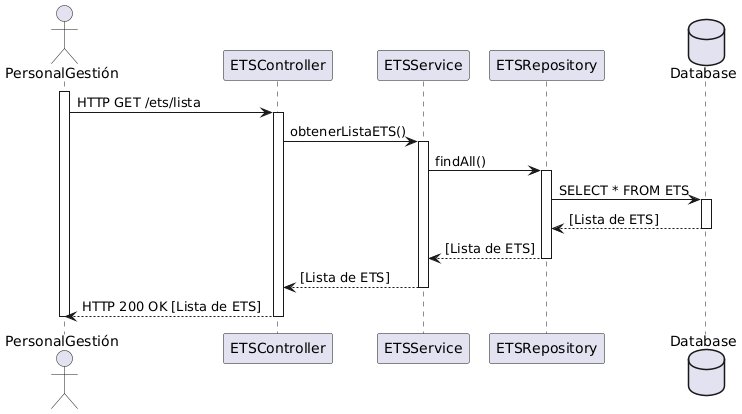
\includegraphics[width=.35\textwidth]{Secuencia/CU-28.png}}
		\caption{Diagrama de secuencia del caso de uso número 28 (CU-28).}
		\label{fig:Diagrama de secuencia CU-28}
	\end{center}
\end{figure}

\begin{figure}[htbp!]
	\begin{center}
		\fbox{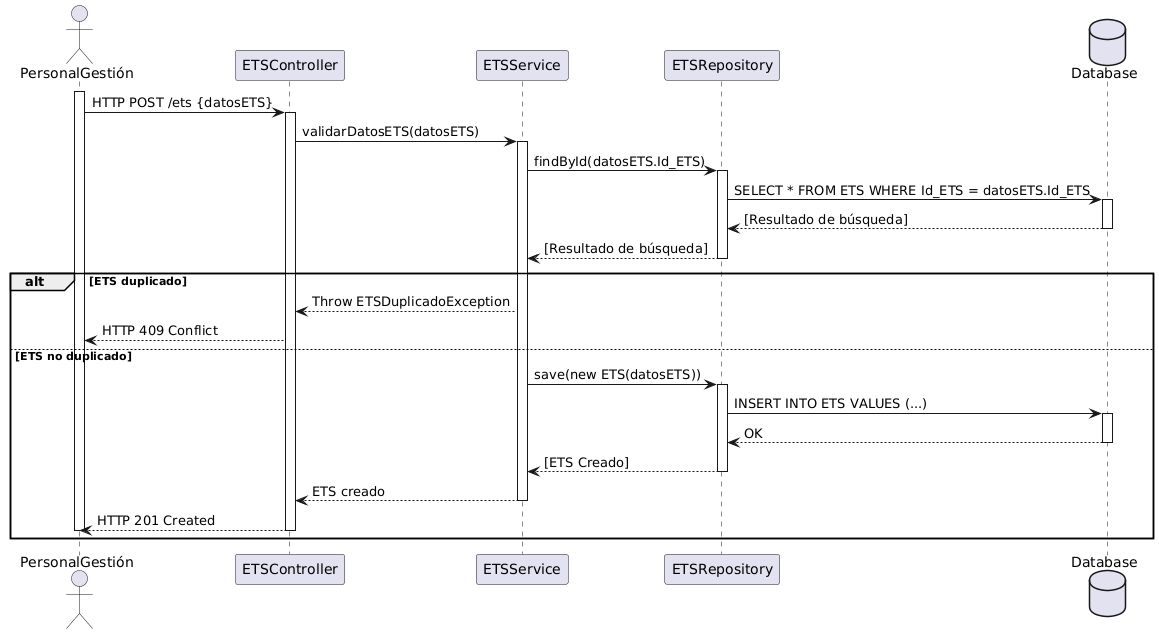
\includegraphics[width=.35\textwidth]{Secuencia/CU-29.png}}
		\caption{Diagrama de secuencia del caso de uso número 29 (CU-29).}
		\label{fig:Diagrama de secuencia CU-29}
	\end{center}
\end{figure}

\begin{figure}[htbp!]
	\begin{center}
		\fbox{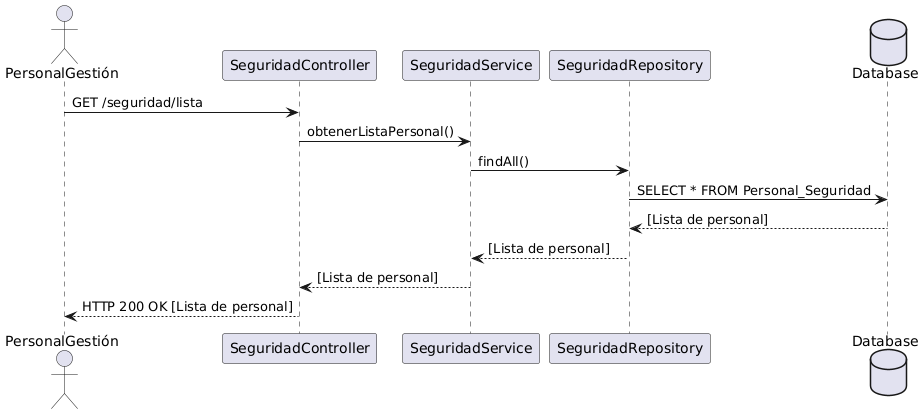
\includegraphics[width=.35\textwidth]{Secuencia/CU-32.png}}
		\caption{Diagrama de secuencia del caso de uso número 32 (CU-32).}
		\label{fig:Diagrama de secuencia CU-32}
	\end{center}
\end{figure}

\begin{figure}[htbp!]
	\begin{center}
		\fbox{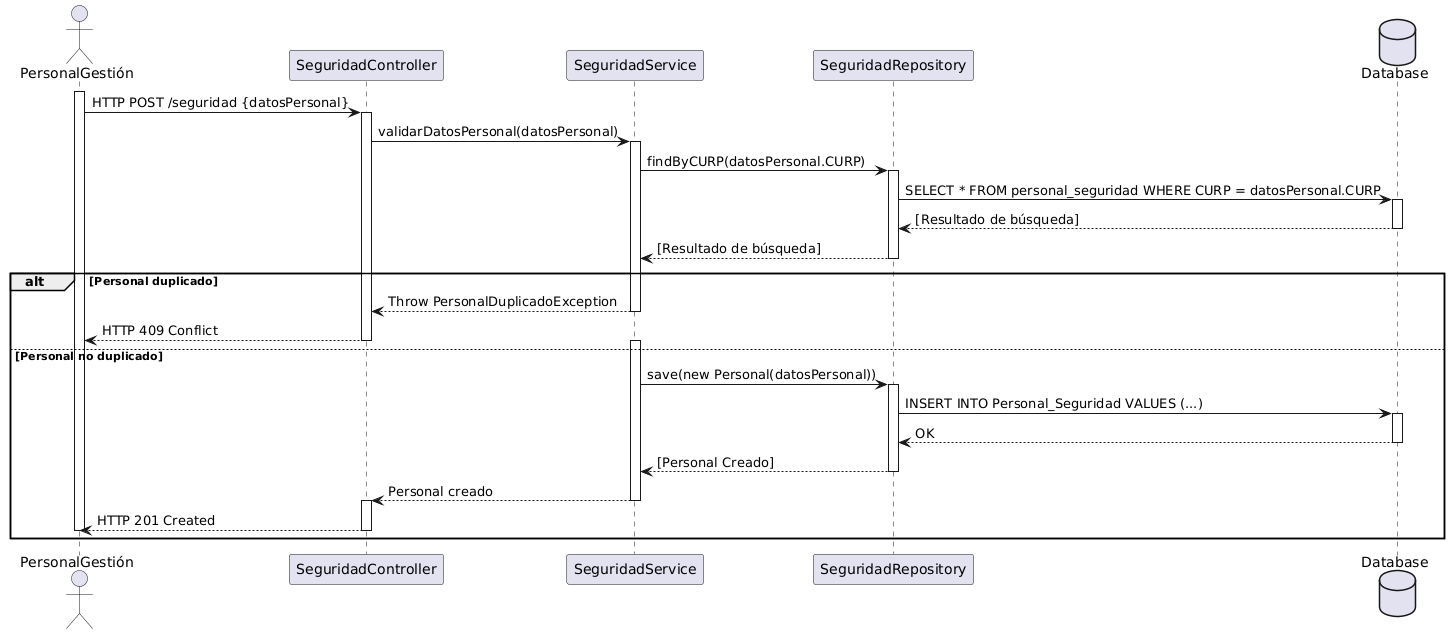
\includegraphics[width=.35\textwidth]{Secuencia/CU-33.png}}
		\caption{Diagrama de secuencia del caso de uso número 33 (CU-33).}
		\label{fig:Diagrama de secuencia CU-33}
	\end{center}
\end{figure}

\begin{figure}[htbp!]
	\begin{center}
		\fbox{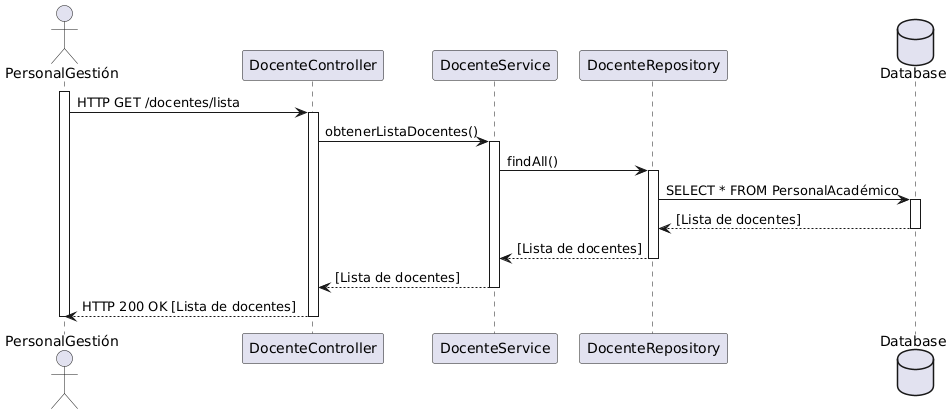
\includegraphics[width=.35\textwidth]{Secuencia/CU-36.png}}
		\caption{Diagrama de secuencia del caso de uso número 36 (CU-36).}
		\label{fig:Diagrama de secuencia CU-36}
	\end{center}
\end{figure}

\begin{figure}[htbp!]
	\begin{center}
		\fbox{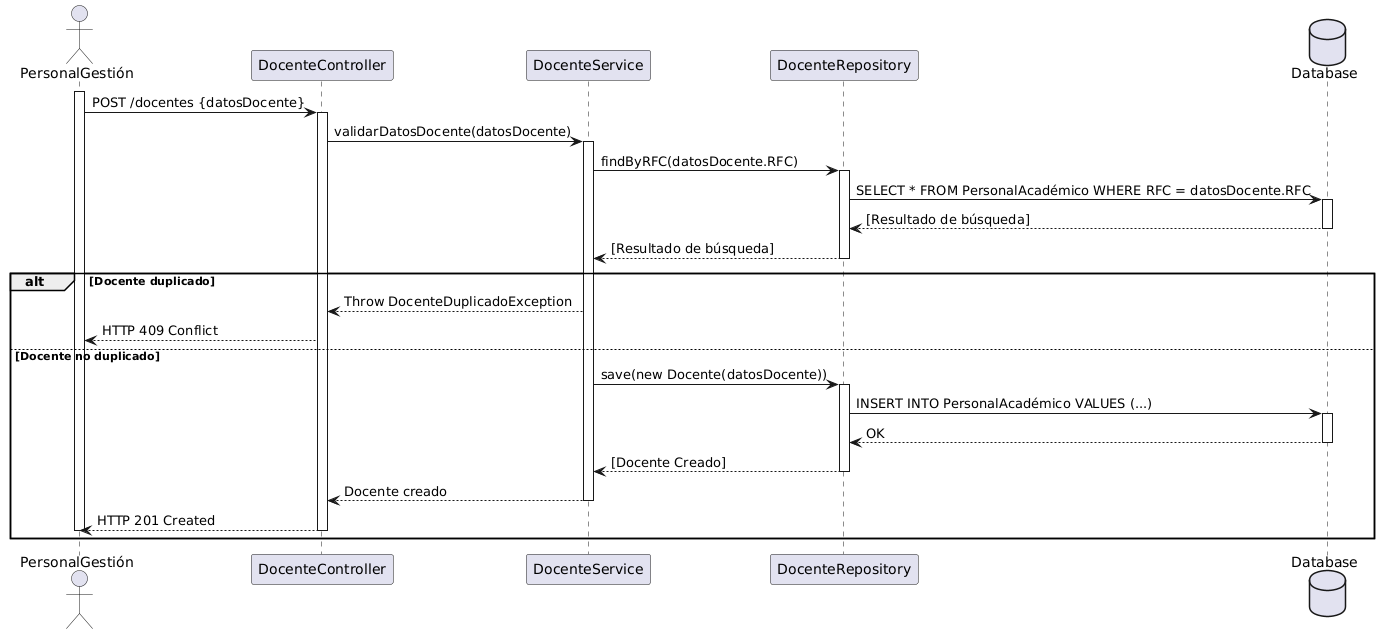
\includegraphics[width=.35\textwidth]{Secuencia/CU-37.png}}
		\caption{Diagrama de secuencia del caso de uso número 37 (CU-37).}
		\label{fig:Diagrama de secuencia CU-37}
	\end{center}
\end{figure}

\begin{figure}[htbp!]
	\begin{center}
		\fbox{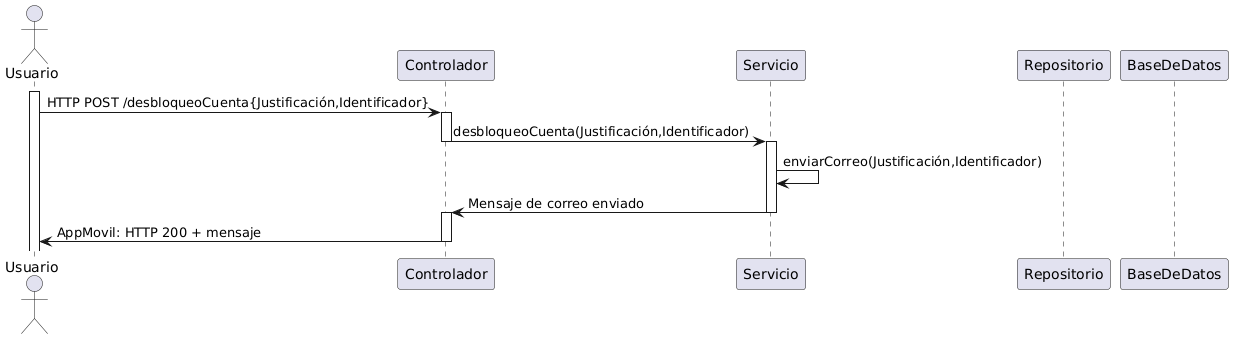
\includegraphics[width=.35\textwidth]{Secuencia/CU-40.png}}
		\caption{Diagrama de secuencia del caso de uso número 40 (CU-40).}
		\label{fig:Diagrama de secuencia CU-40}
	\end{center}
\end{figure}

\begin{figure}[htbp!]
	\begin{center}
		\fbox{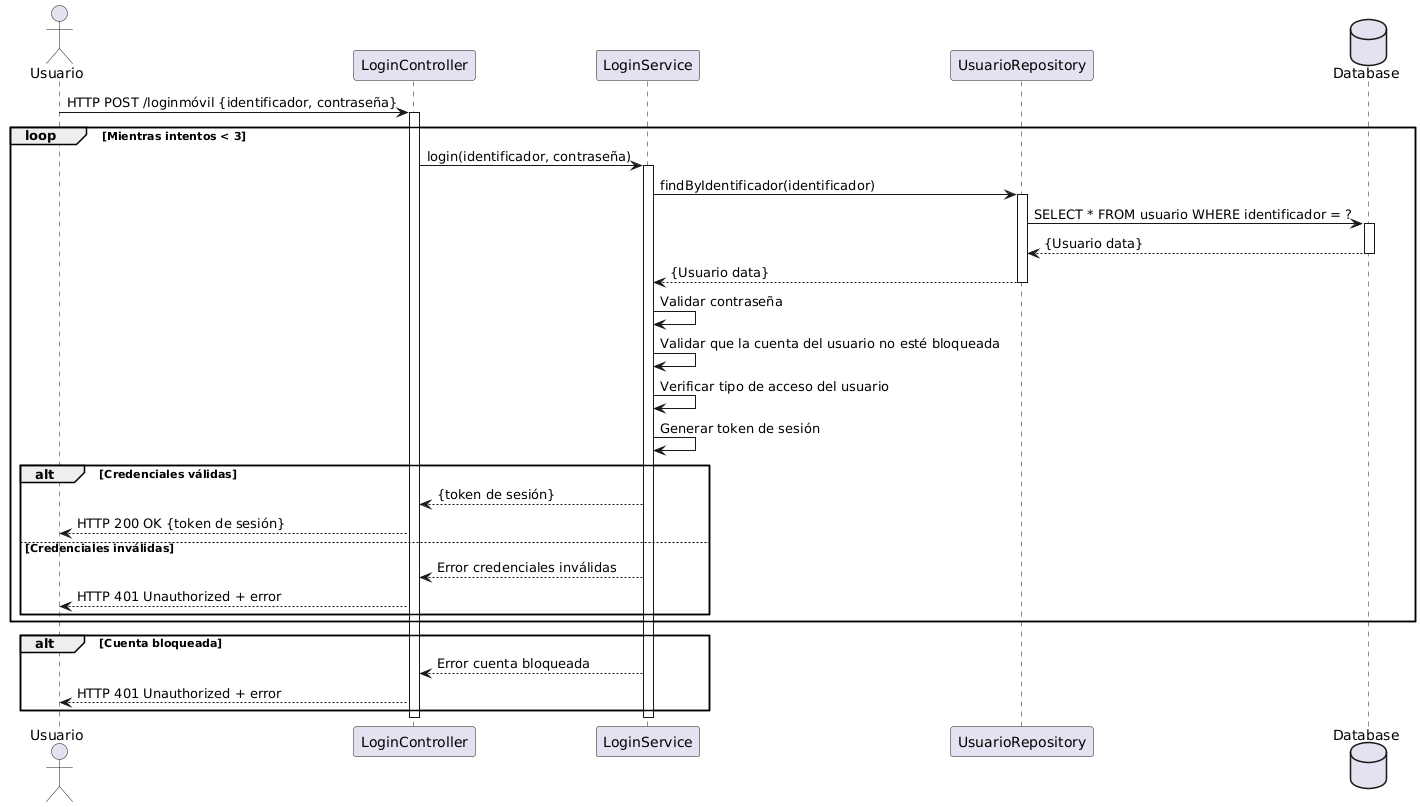
\includegraphics[width=.35\textwidth]{Secuencia/CU-41.png}}
		\caption{Diagrama de secuencia del caso de uso número 41 (CU-41).}
		\label{fig:Diagrama de secuencia CU-41}
	\end{center}
\end{figure}

\begin{figure}[htbp!]
	\begin{center}
		\fbox{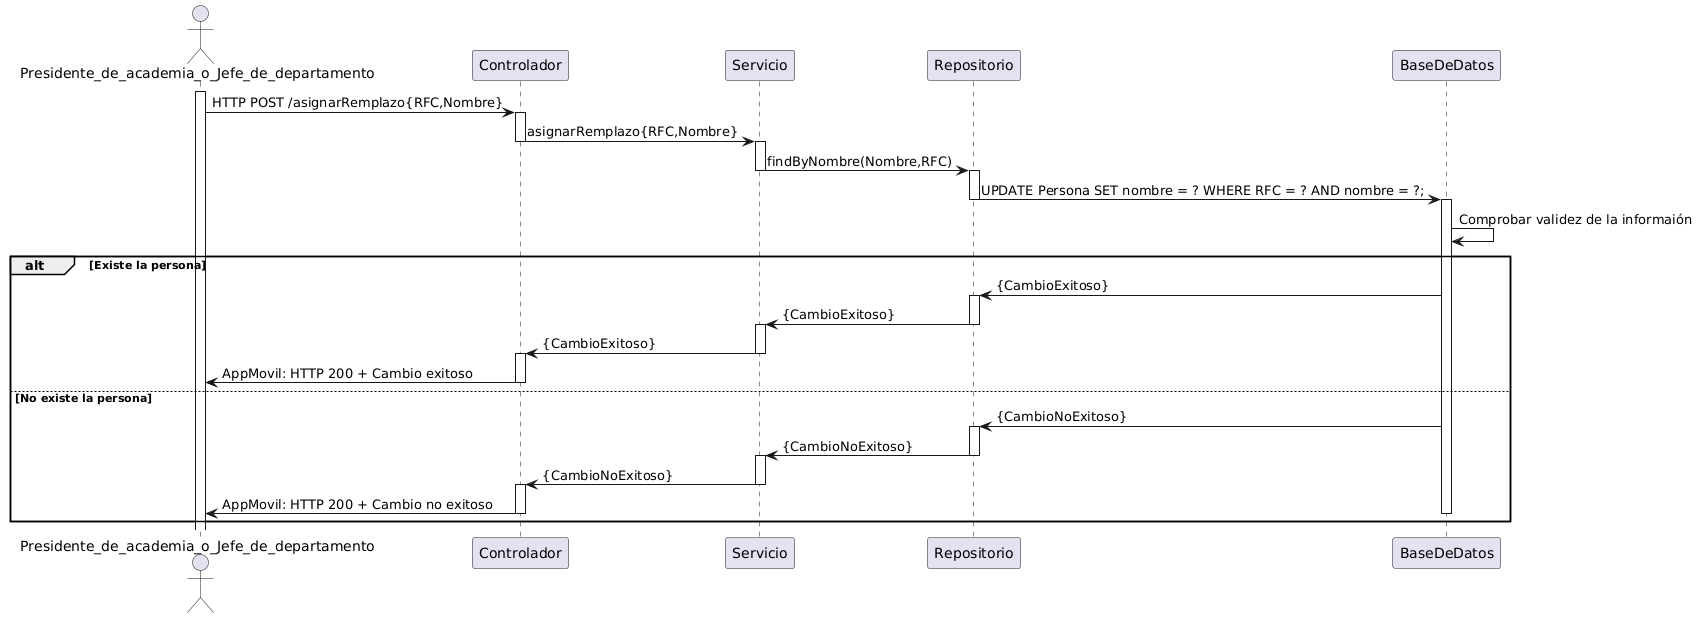
\includegraphics[width=.35\textwidth]{Secuencia/CU-42.png}}
		\caption{Diagrama de secuencia del caso de uso número 42 (CU-42).}
		\label{fig:Diagrama de secuencia CU-42}
	\end{center}
\end{figure}

\bibliography{ref}

\end{document}